%% USPSC-Apendice.tex
% ---
% Inicia os apêndices
% ---

\begin{apendicesenv}
% Imprime uma página indicando o início dos apêndices

\partapendices

\chapter{Gráficos de \textit{throughput}, desempenho e \textit{Round Trip Time} (RTT) em diferentes cenários da comunicação OPC UA}

\begin{figure}[htbp!]
    \centering
    \begin{subfigure}[t]{0.5\textwidth}
        \centering
        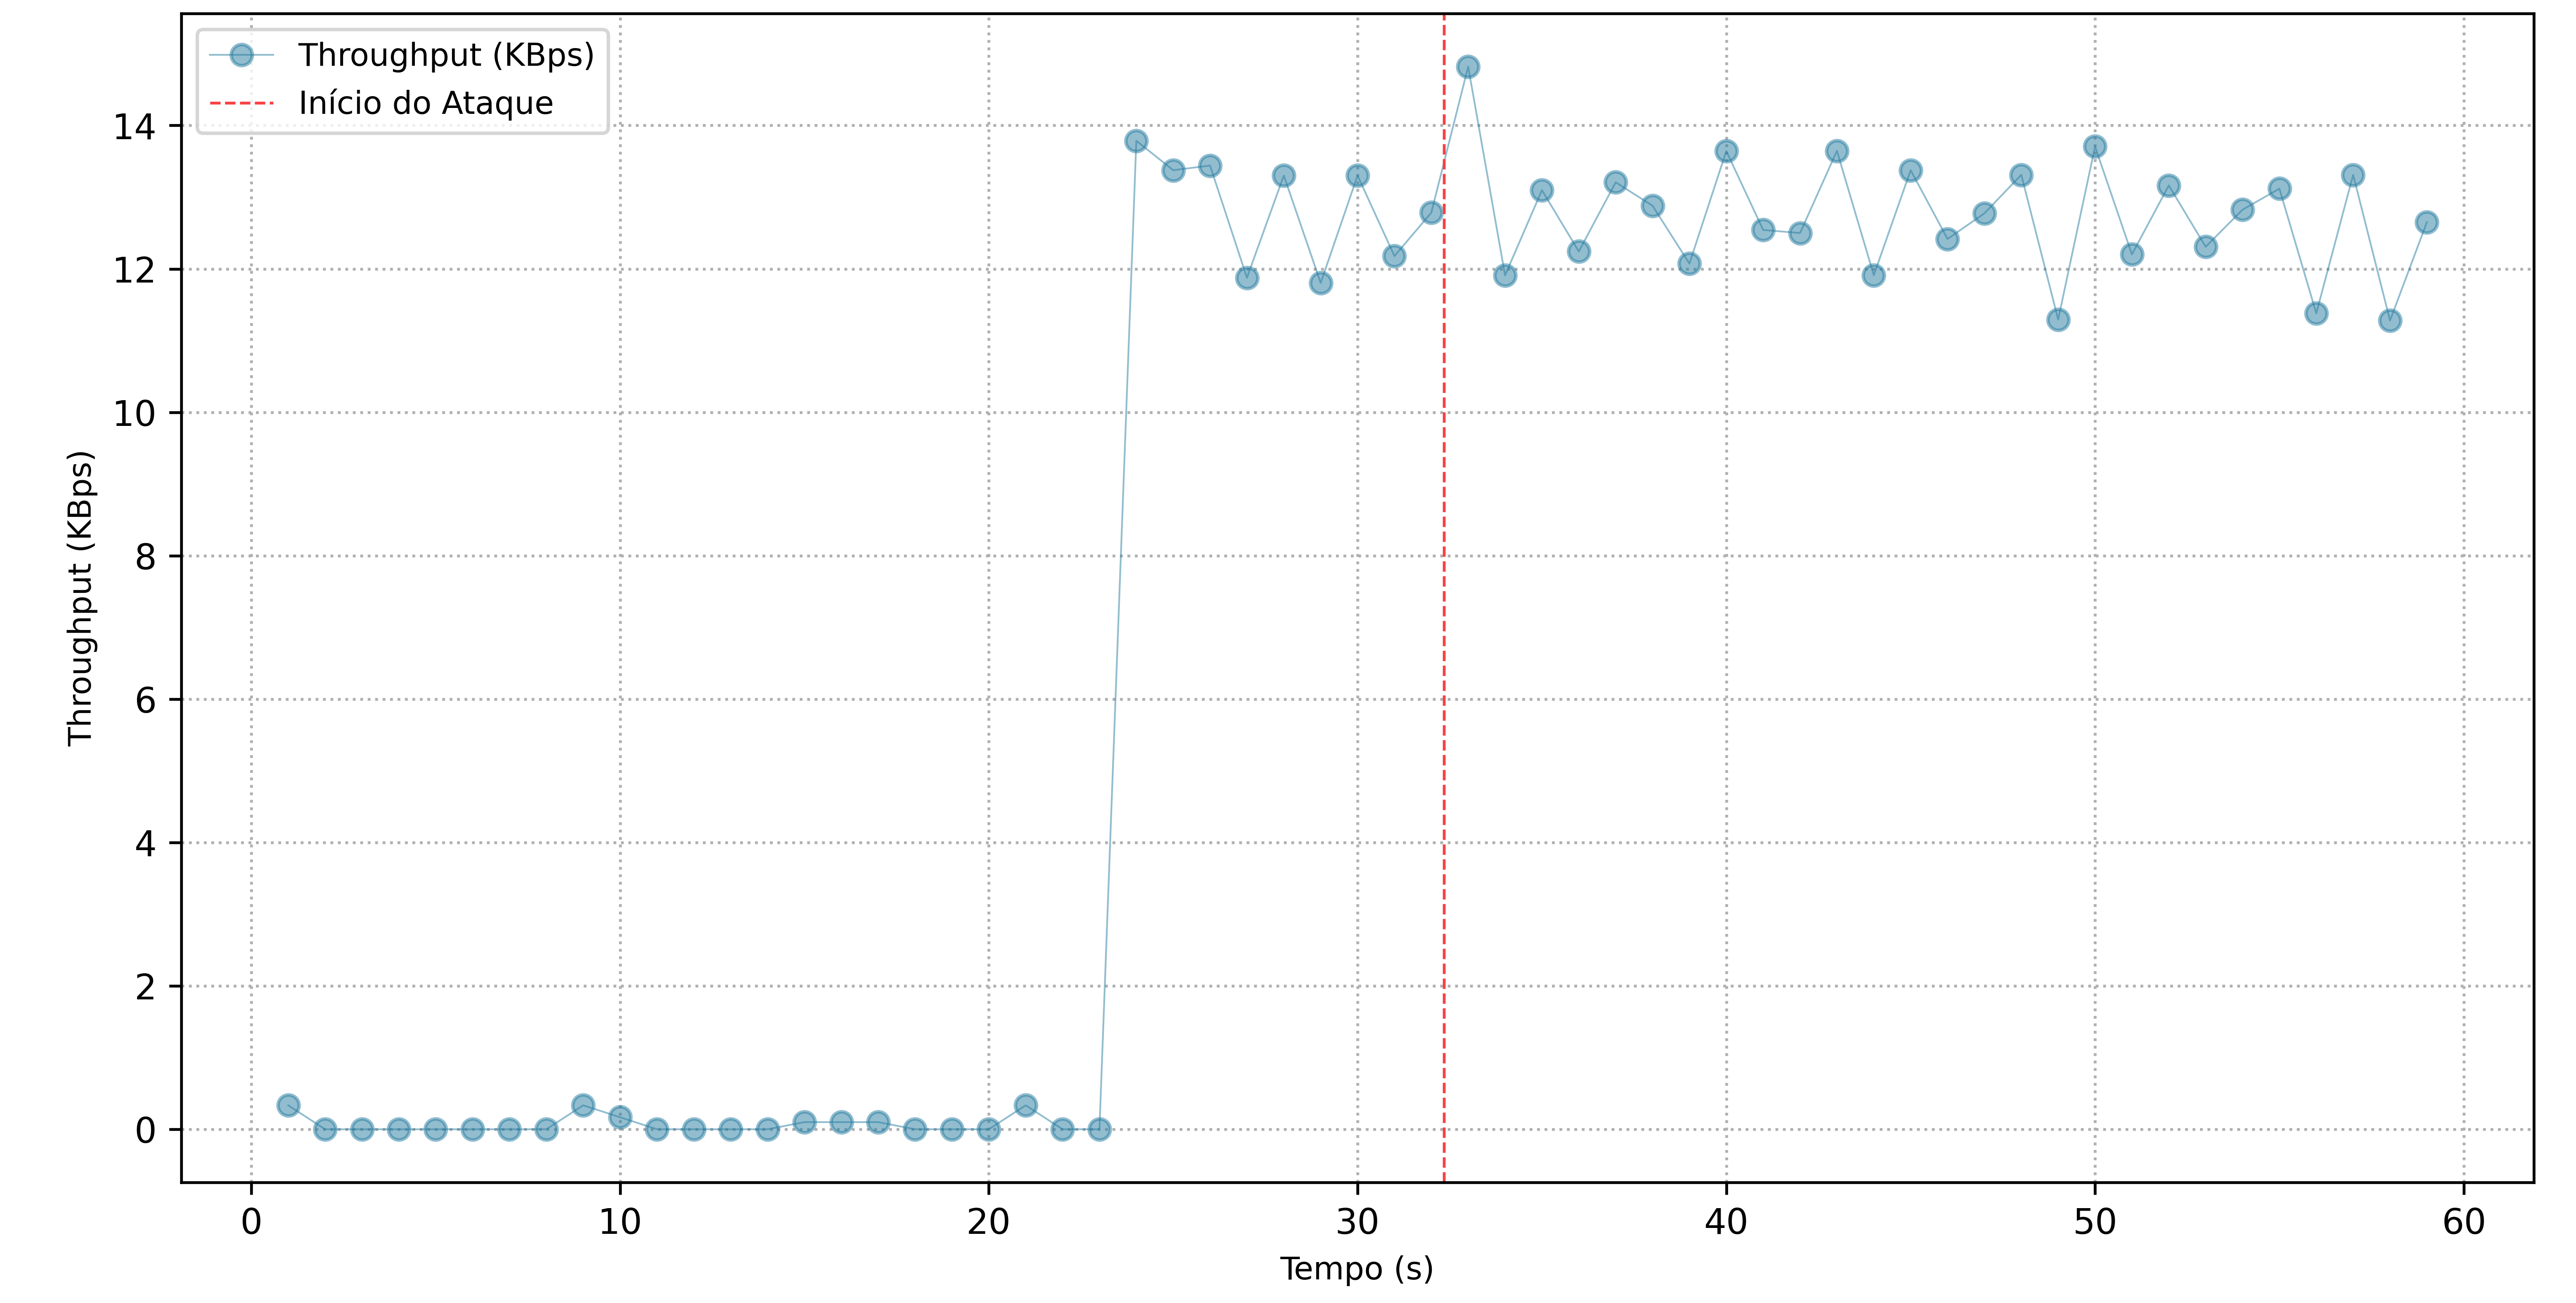
\includegraphics[width=1\textwidth, height=120pt]{USPSC-img/output/cropped/0-dos_certificate_inf_chain_loop-tput.png}
        \caption{\textit{Throughput}}
    \end{subfigure}%
    ~ 
    \begin{subfigure}[t]{0.5\textwidth}
        \centering
        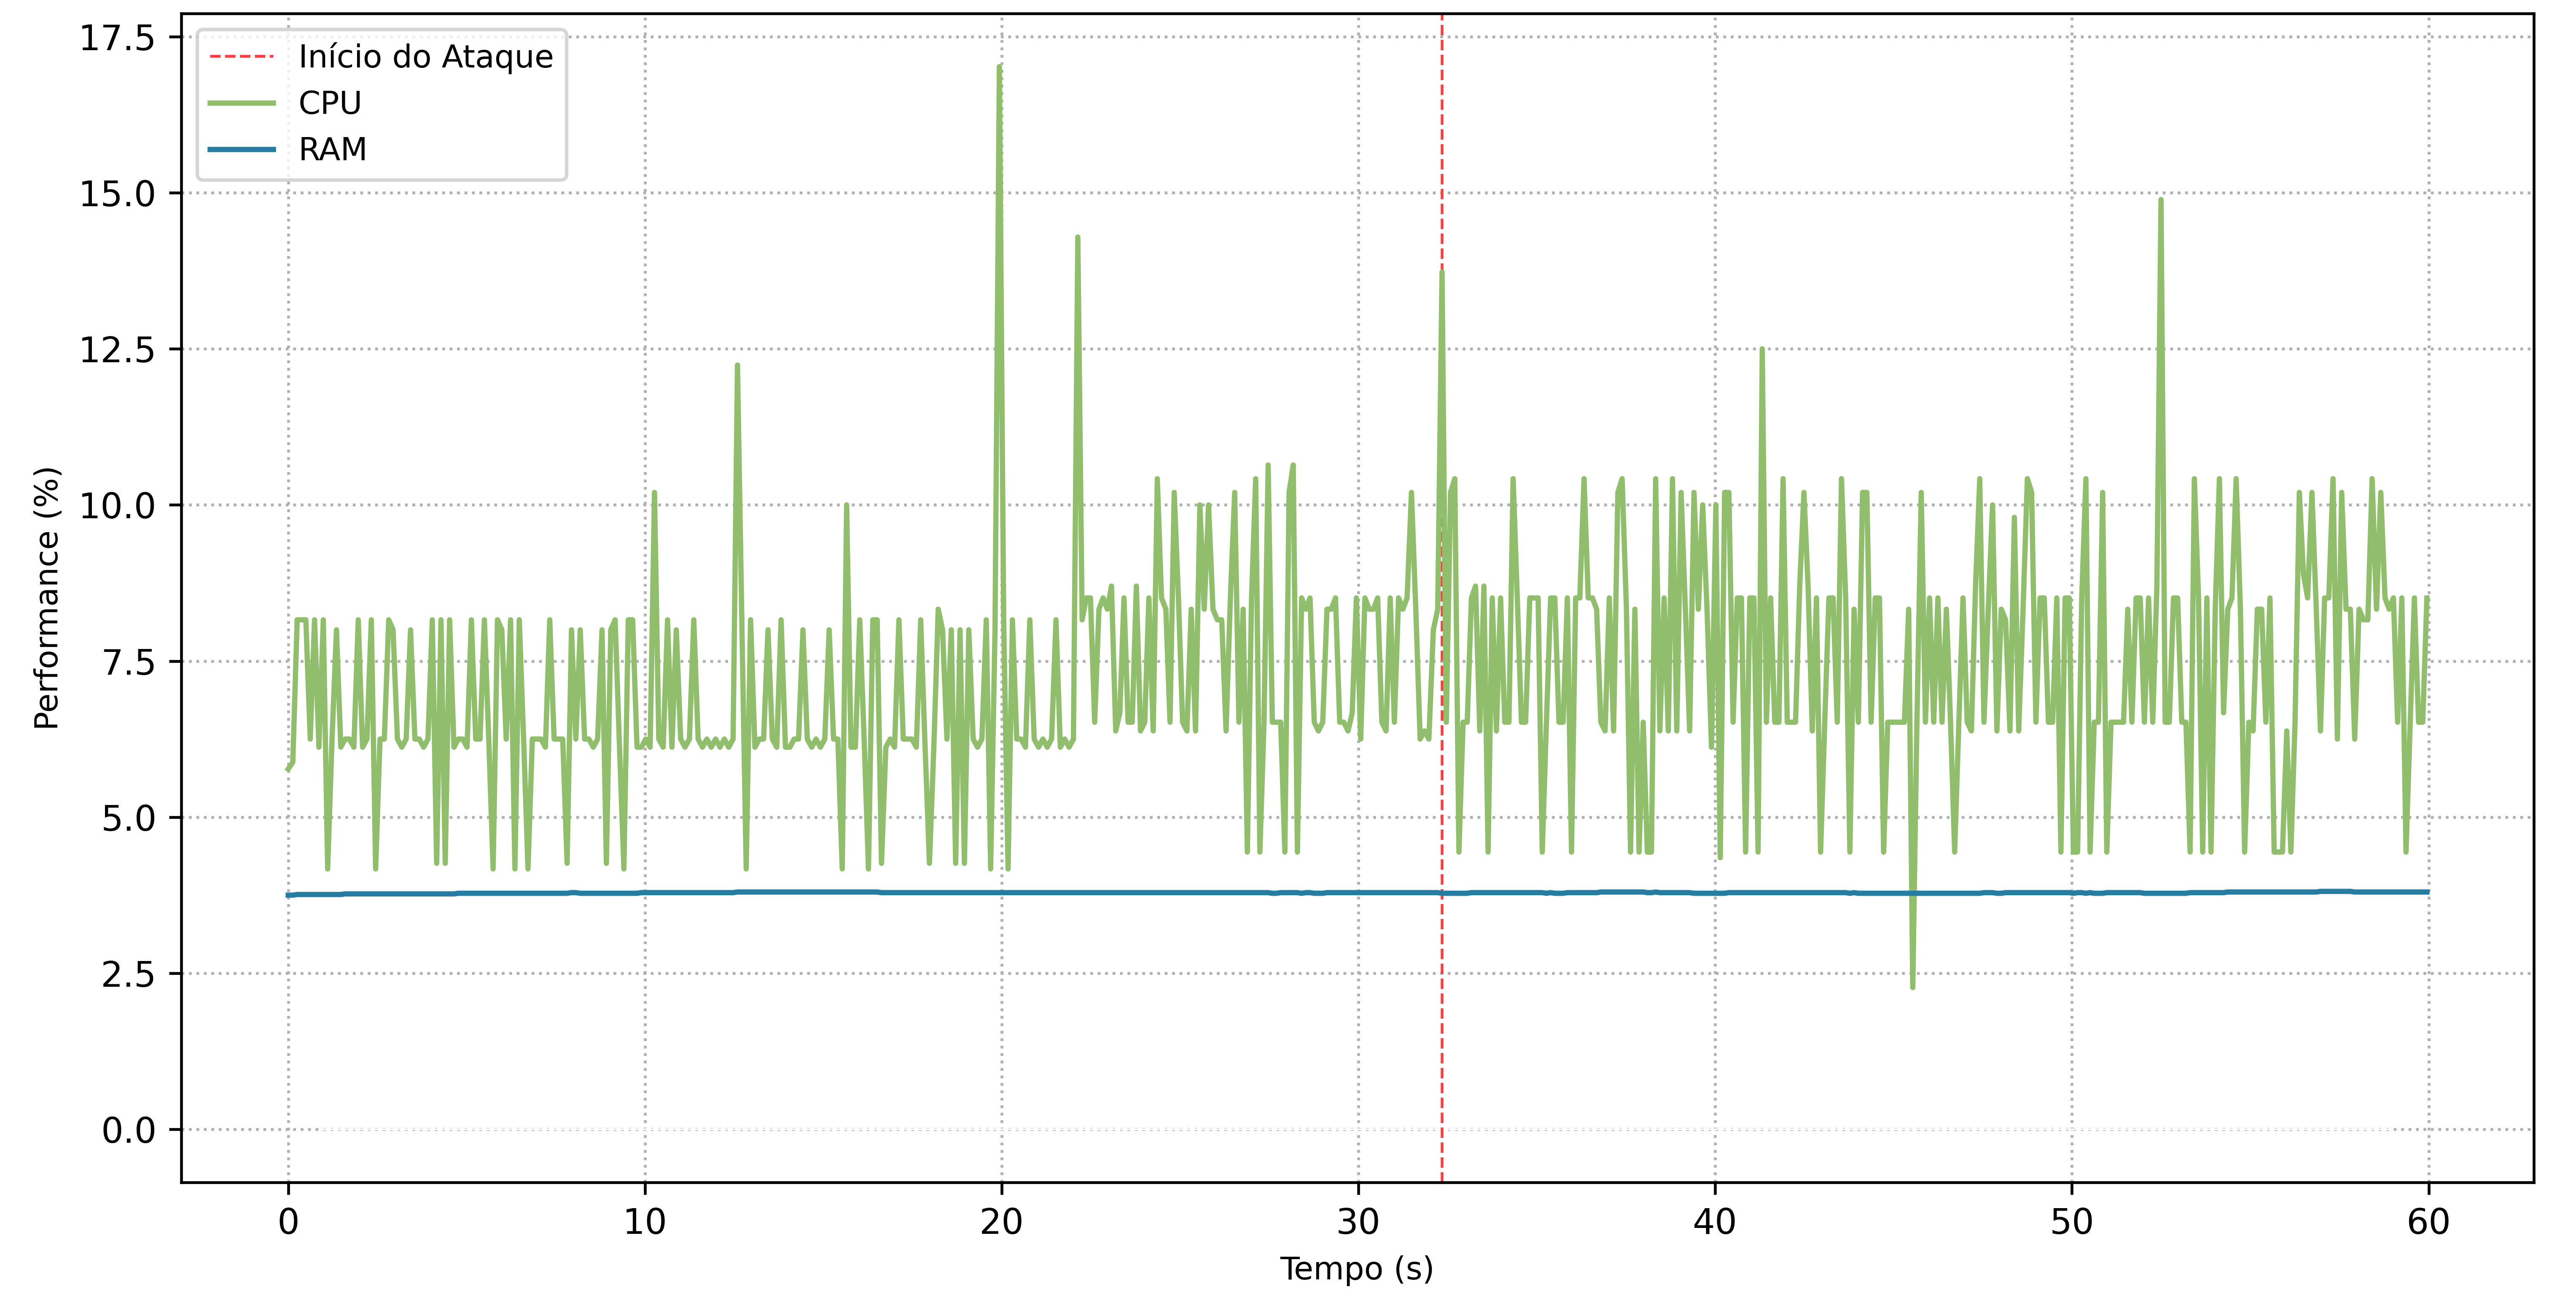
\includegraphics[width=1\textwidth, height=120pt]{USPSC-img/output/cropped/0-dos_certificate_inf_chain_loop-perf.png}
        \caption{Desempenho}
    \end{subfigure}%
    \\
    \begin{subfigure}[t]{0.5\textwidth}
        \centering
        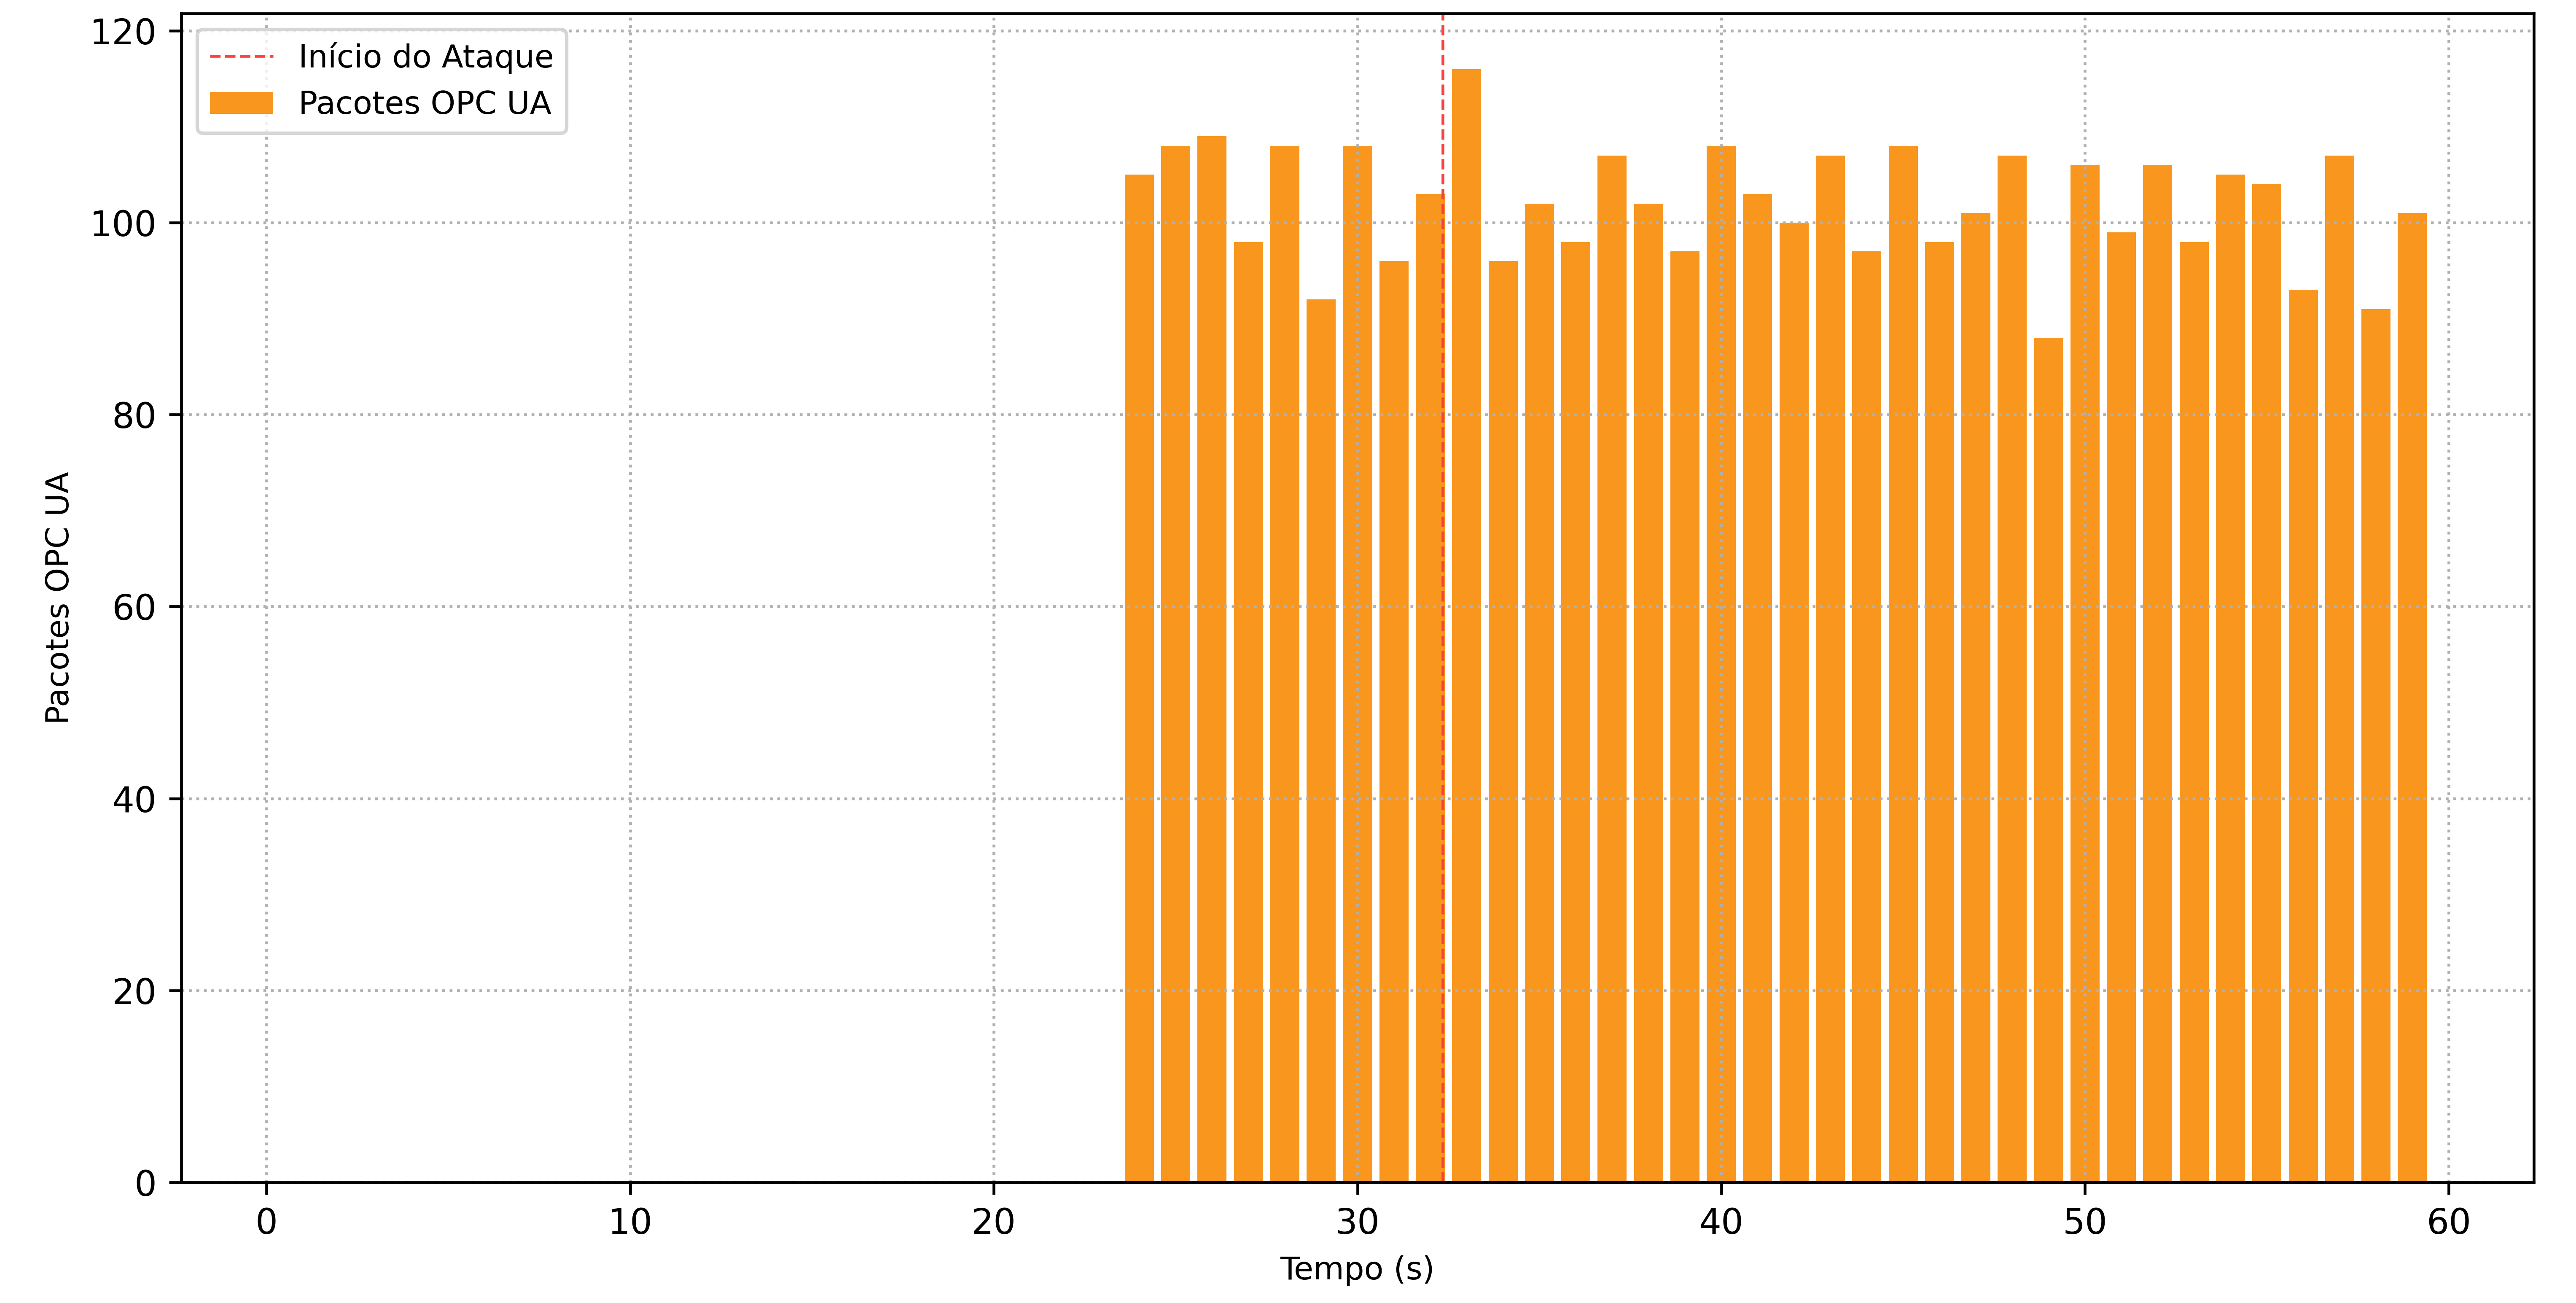
\includegraphics[width=1\textwidth, height=120pt]{USPSC-img/output/cropped/0-dos_certificate_inf_chain_loop-pack.png}
        \caption{Pacotes OPC UA}
    \end{subfigure}%
    ~
    \begin{subfigure}[t]{0.5\textwidth}
        \centering
        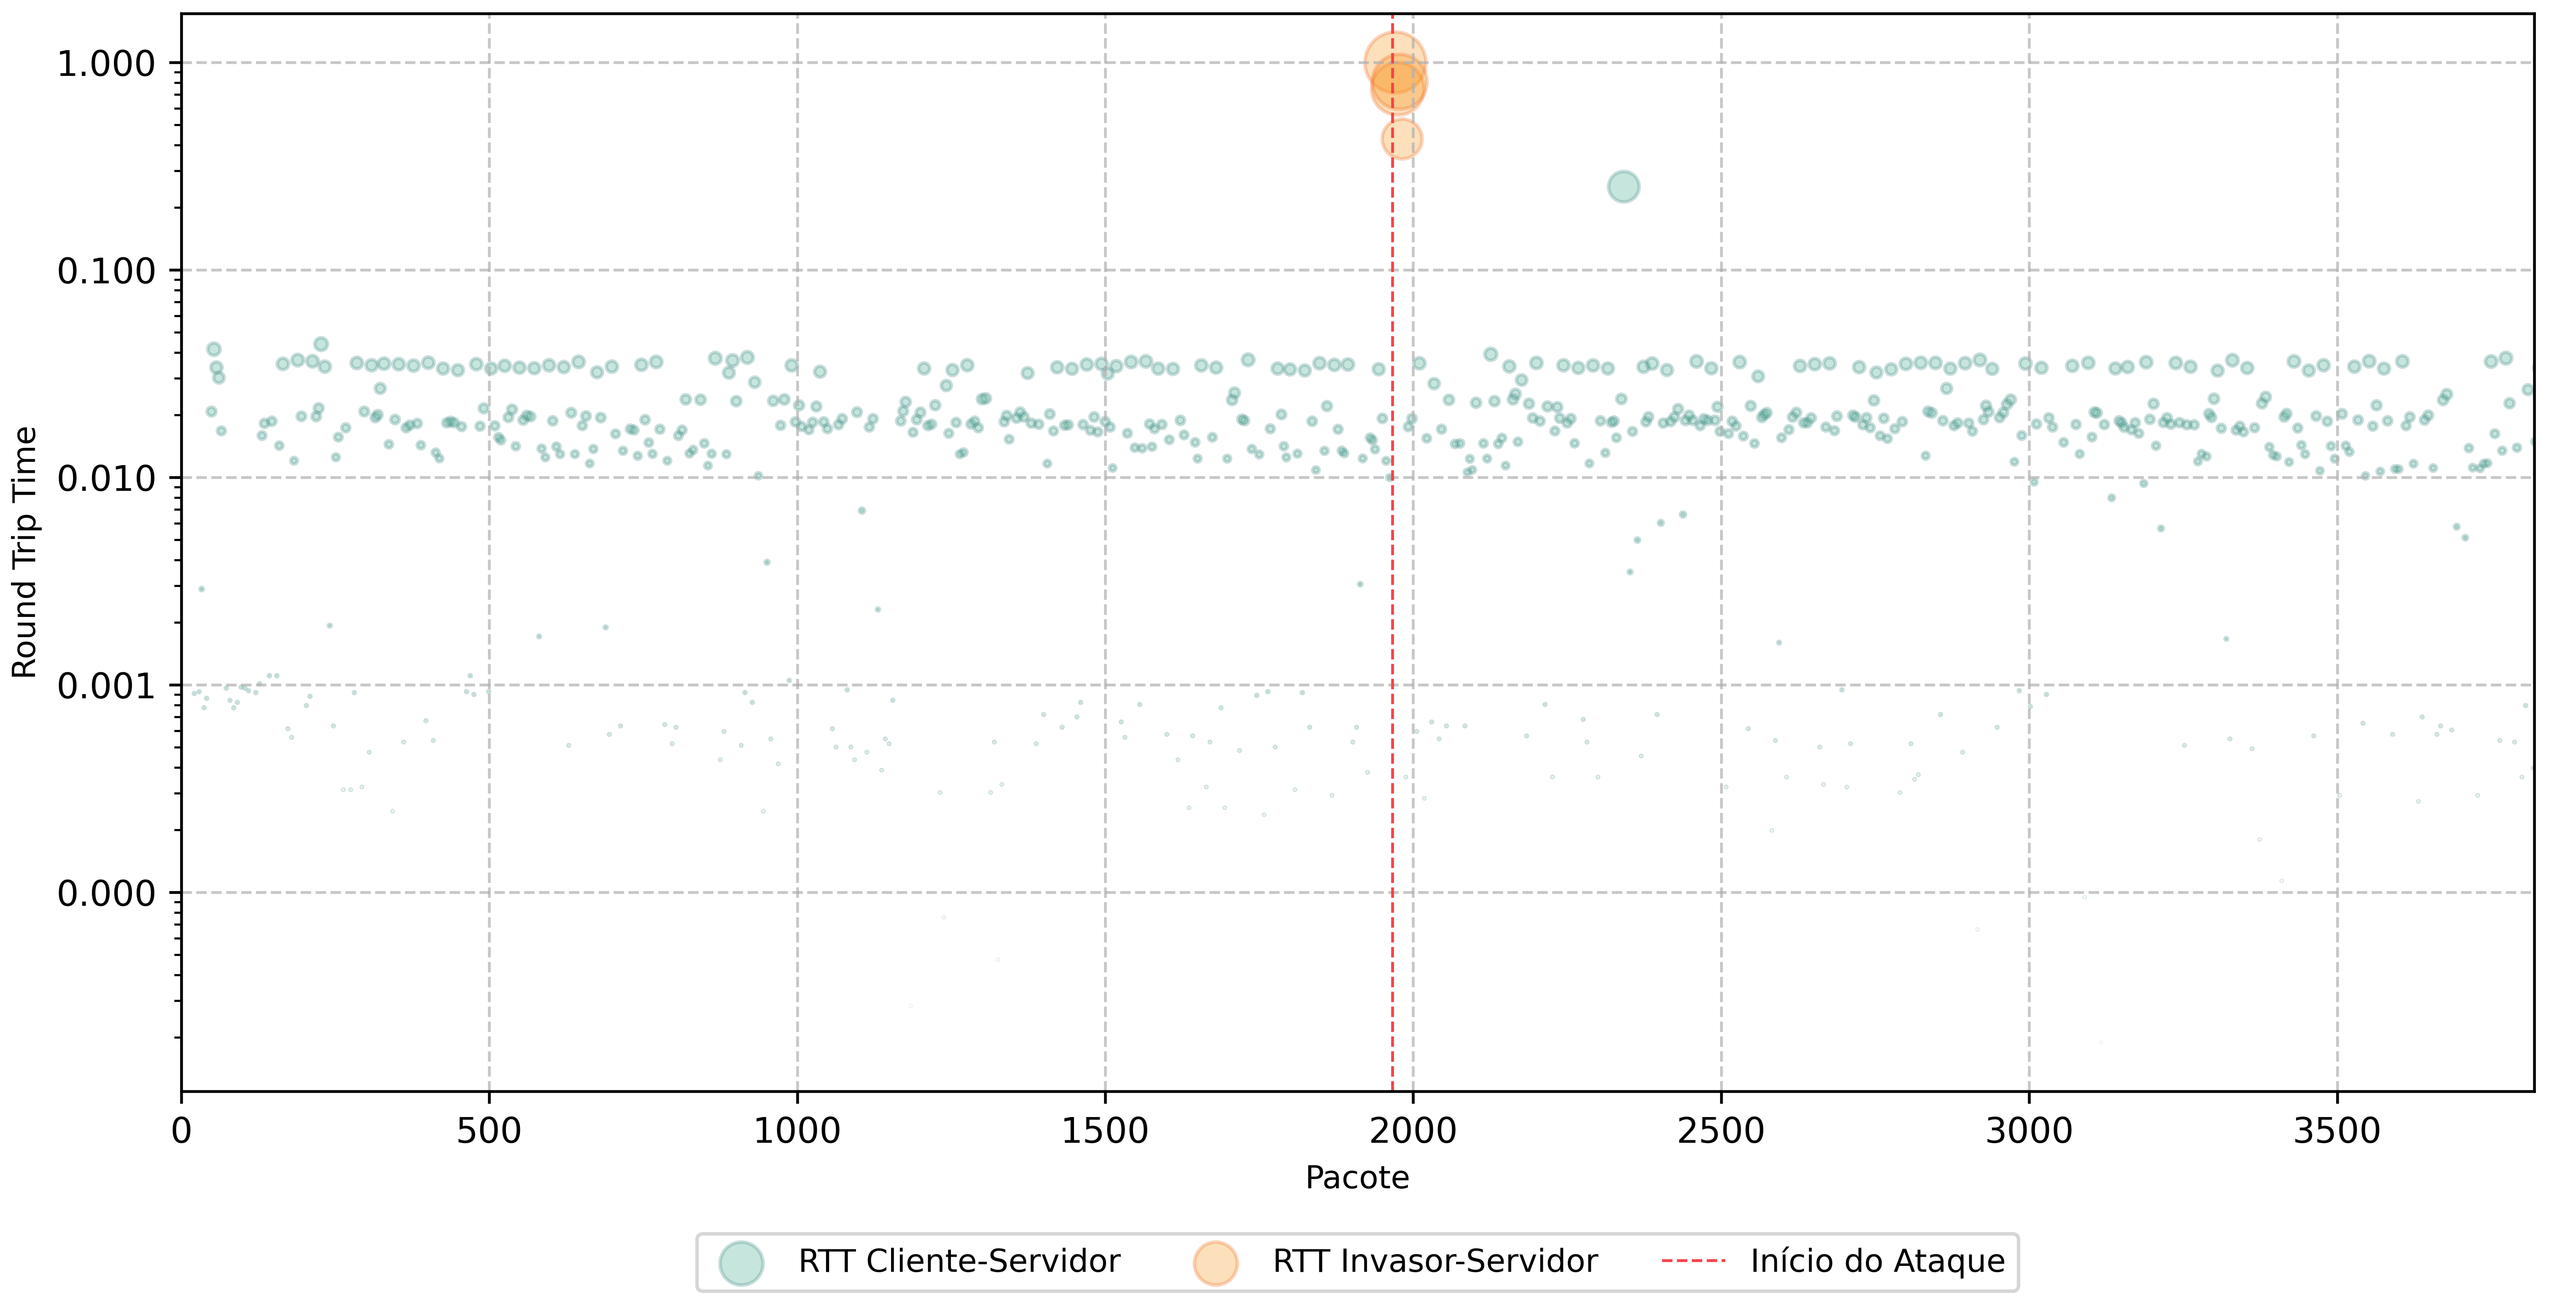
\includegraphics[width=1\textwidth, height=120pt]{USPSC-img/output/cropped/0-dos_certificate_inf_chain_loop-rttp.png}
        \caption{RTT por pacote}
    \end{subfigure}%
    % ~
    % \begin{subfigure}[t]{0.5\textwidth}
    %     \centering
    %     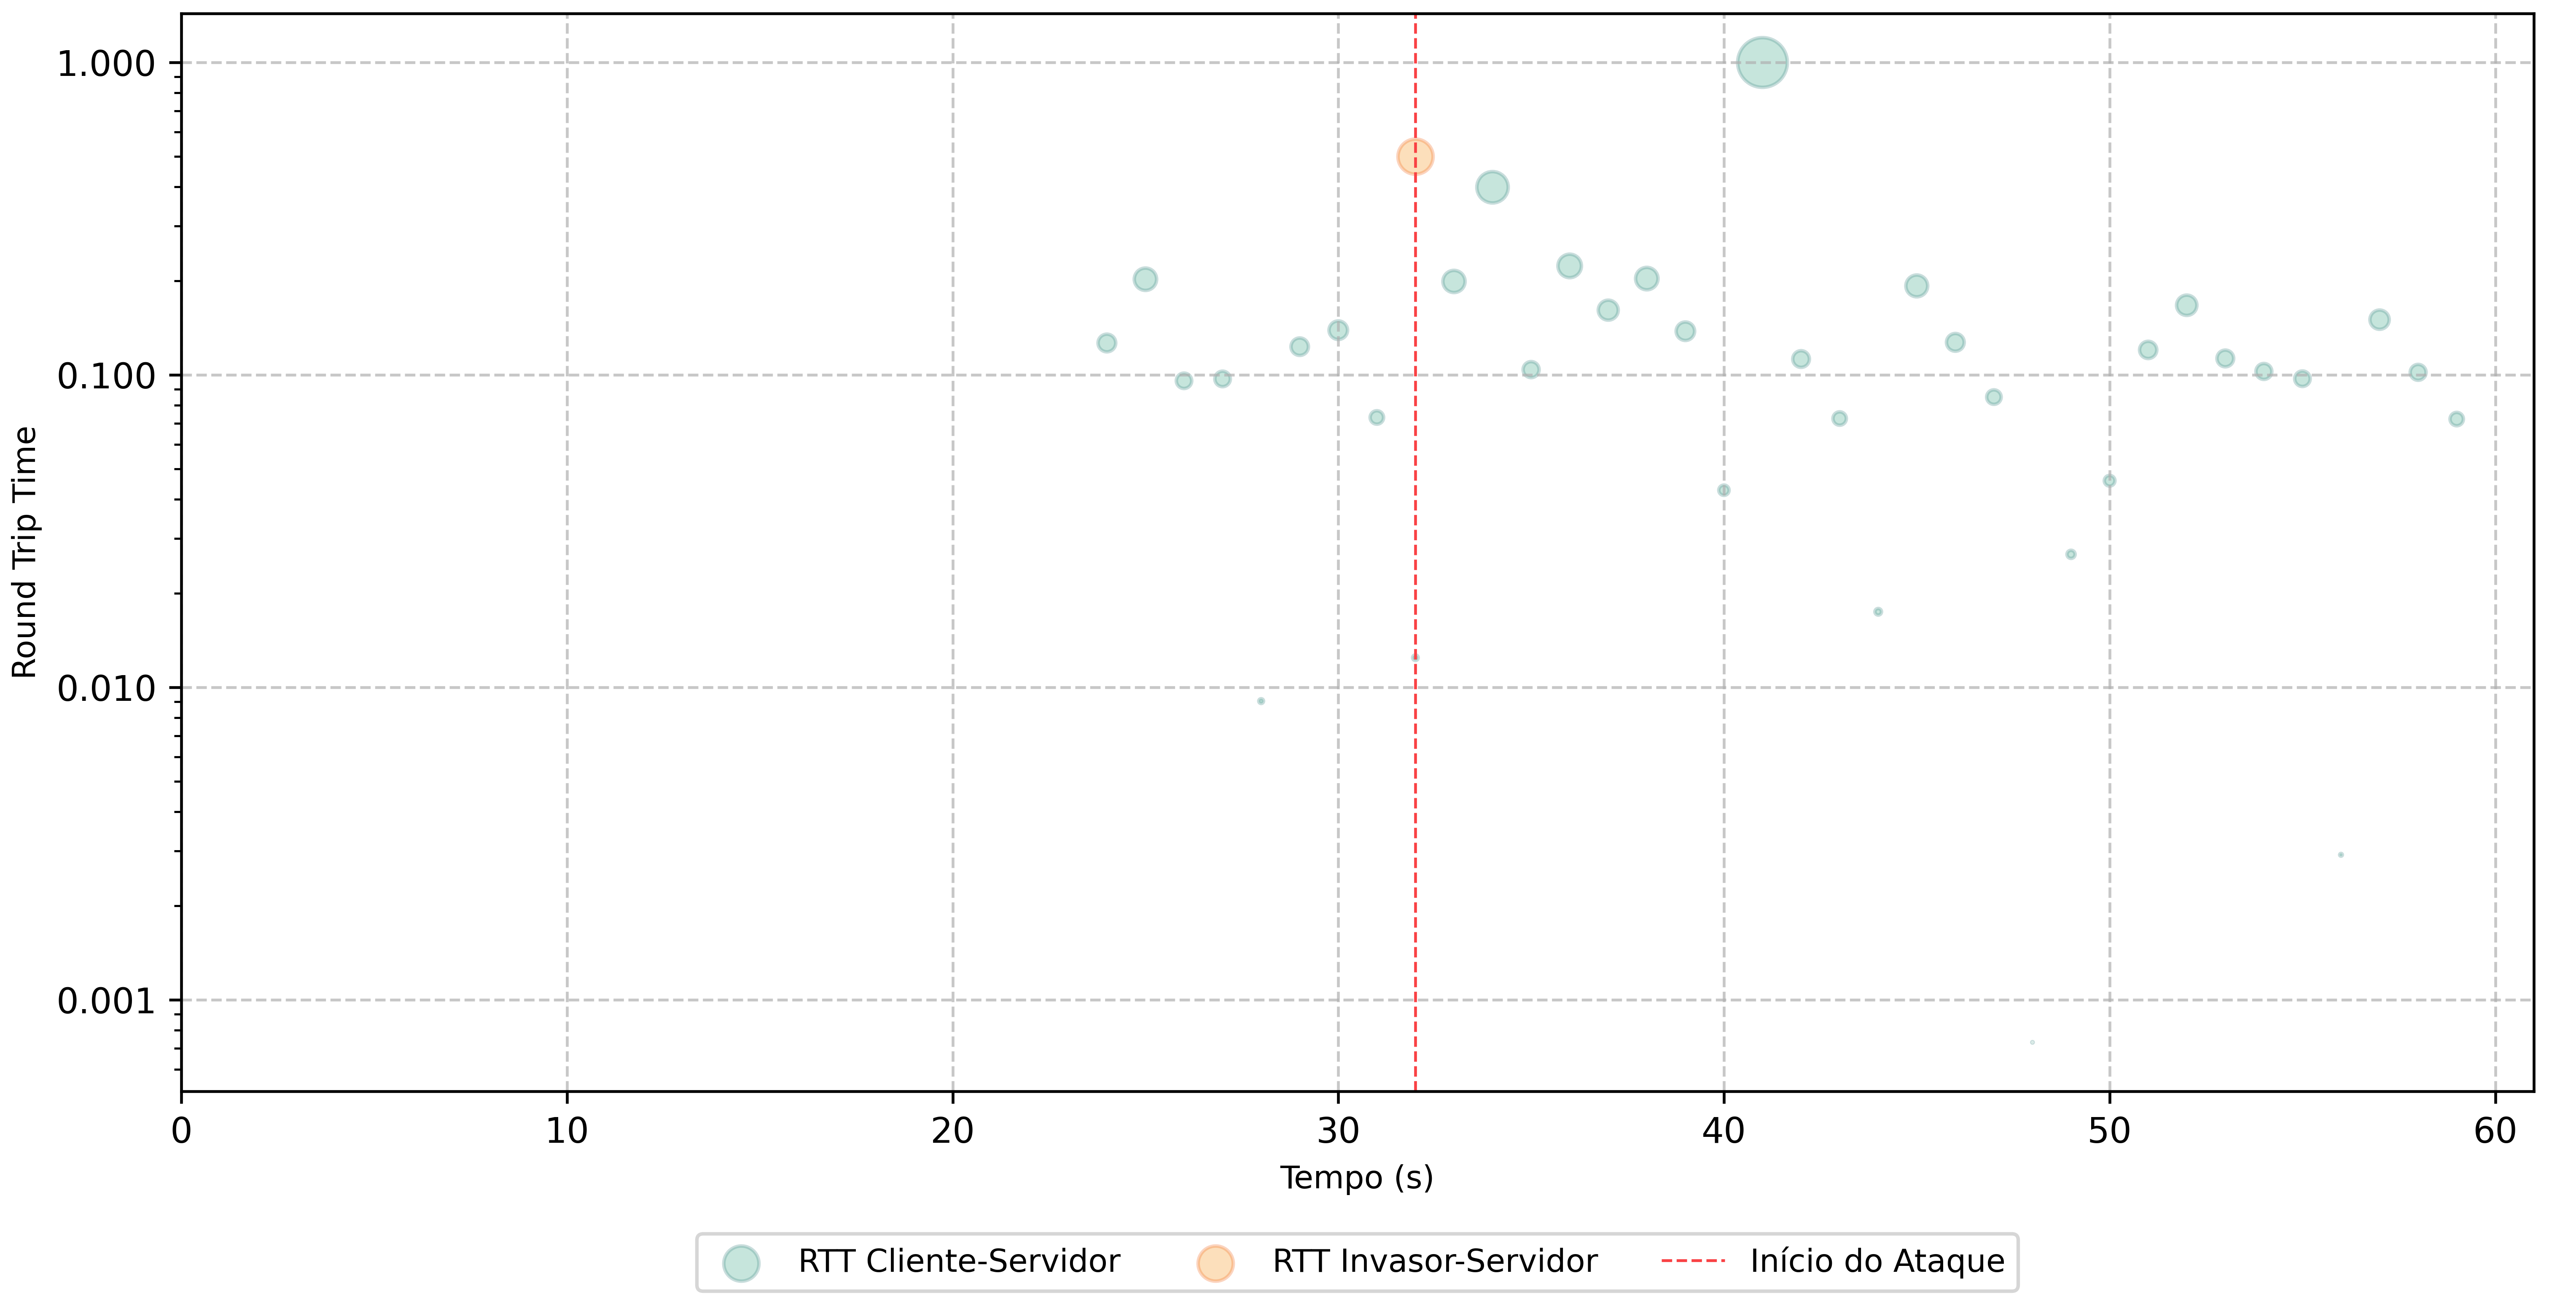
\includegraphics[width=1\textwidth, height=120pt]{USPSC-img/output/cropped/0-dos_certificate_inf_chain_loop-rtts.png}
    %     \caption{RTT por segundos}
    % \end{subfigure}%
    \label{fig:0-dos_certificate_inf_chain_loop}
    \caption{Gráficos do ataque de DoS por loop infinito na cadeia de certificados - nível de segurança: `None'.}
\end{figure}

\begin{figure}[htbp!]
    \centering
    \begin{subfigure}[t]{0.5\textwidth}
        \centering
        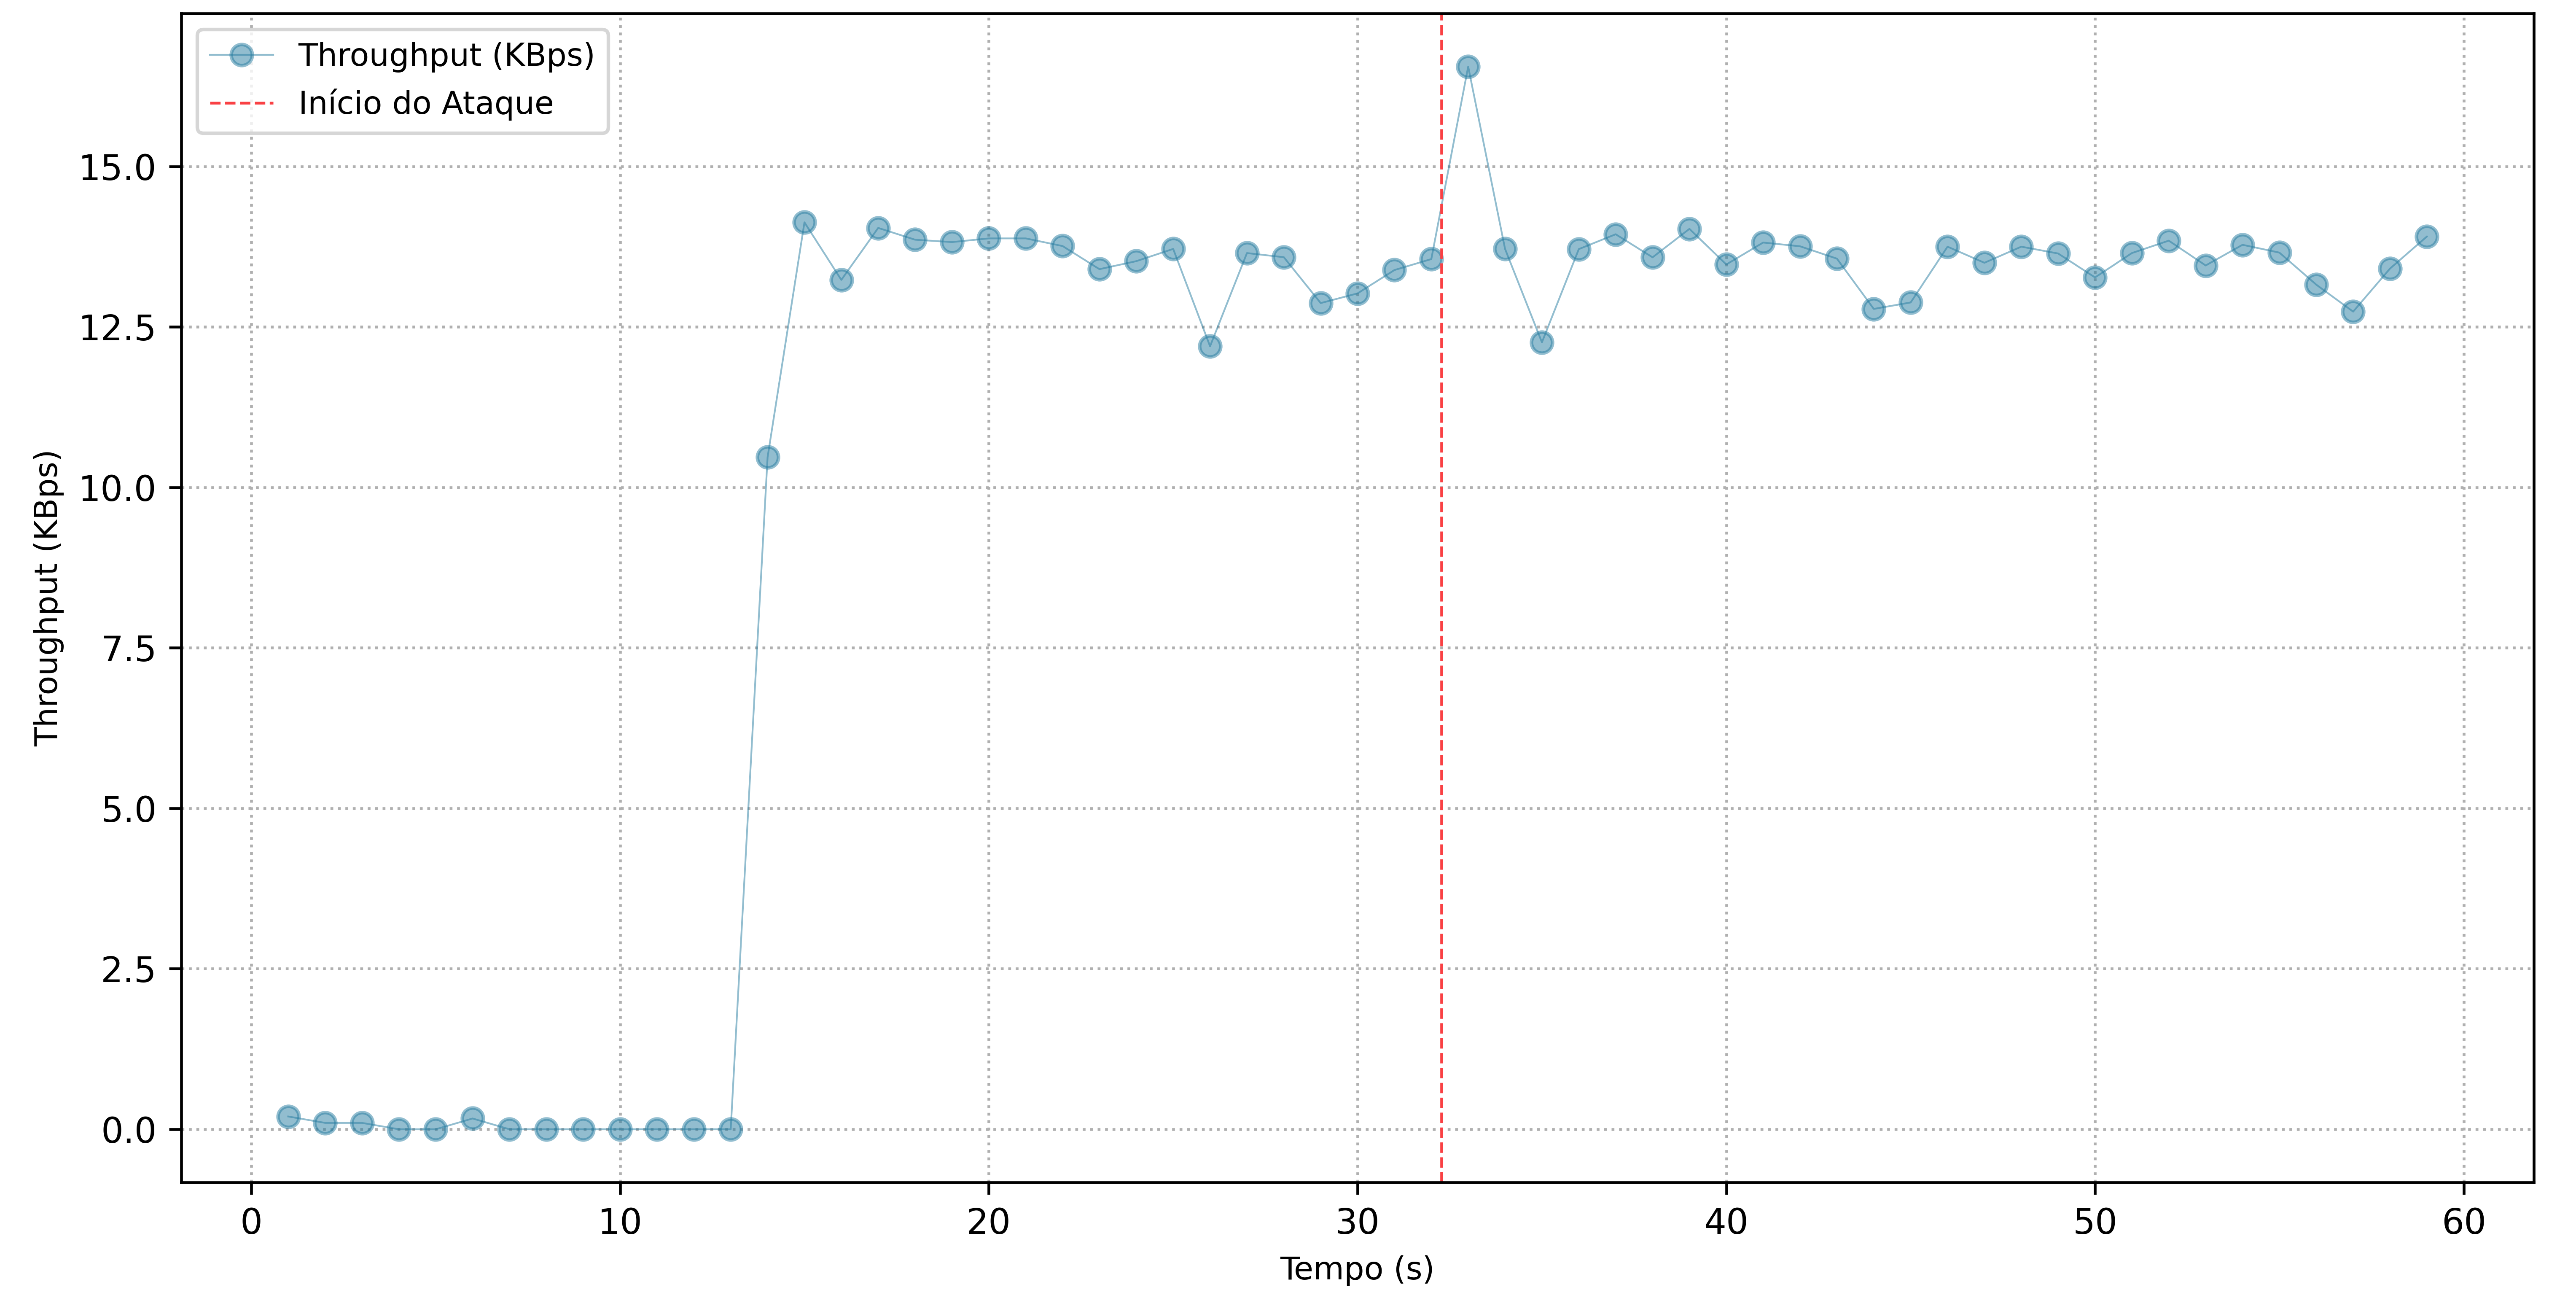
\includegraphics[width=1\textwidth, height=120pt]{USPSC-img/output/cropped/1-dos_certificate_inf_chain_loop-tput.png}
        \caption{\textit{Throughput}}
    \end{subfigure}%
    ~ 
    \begin{subfigure}[t]{0.5\textwidth}
        \centering
        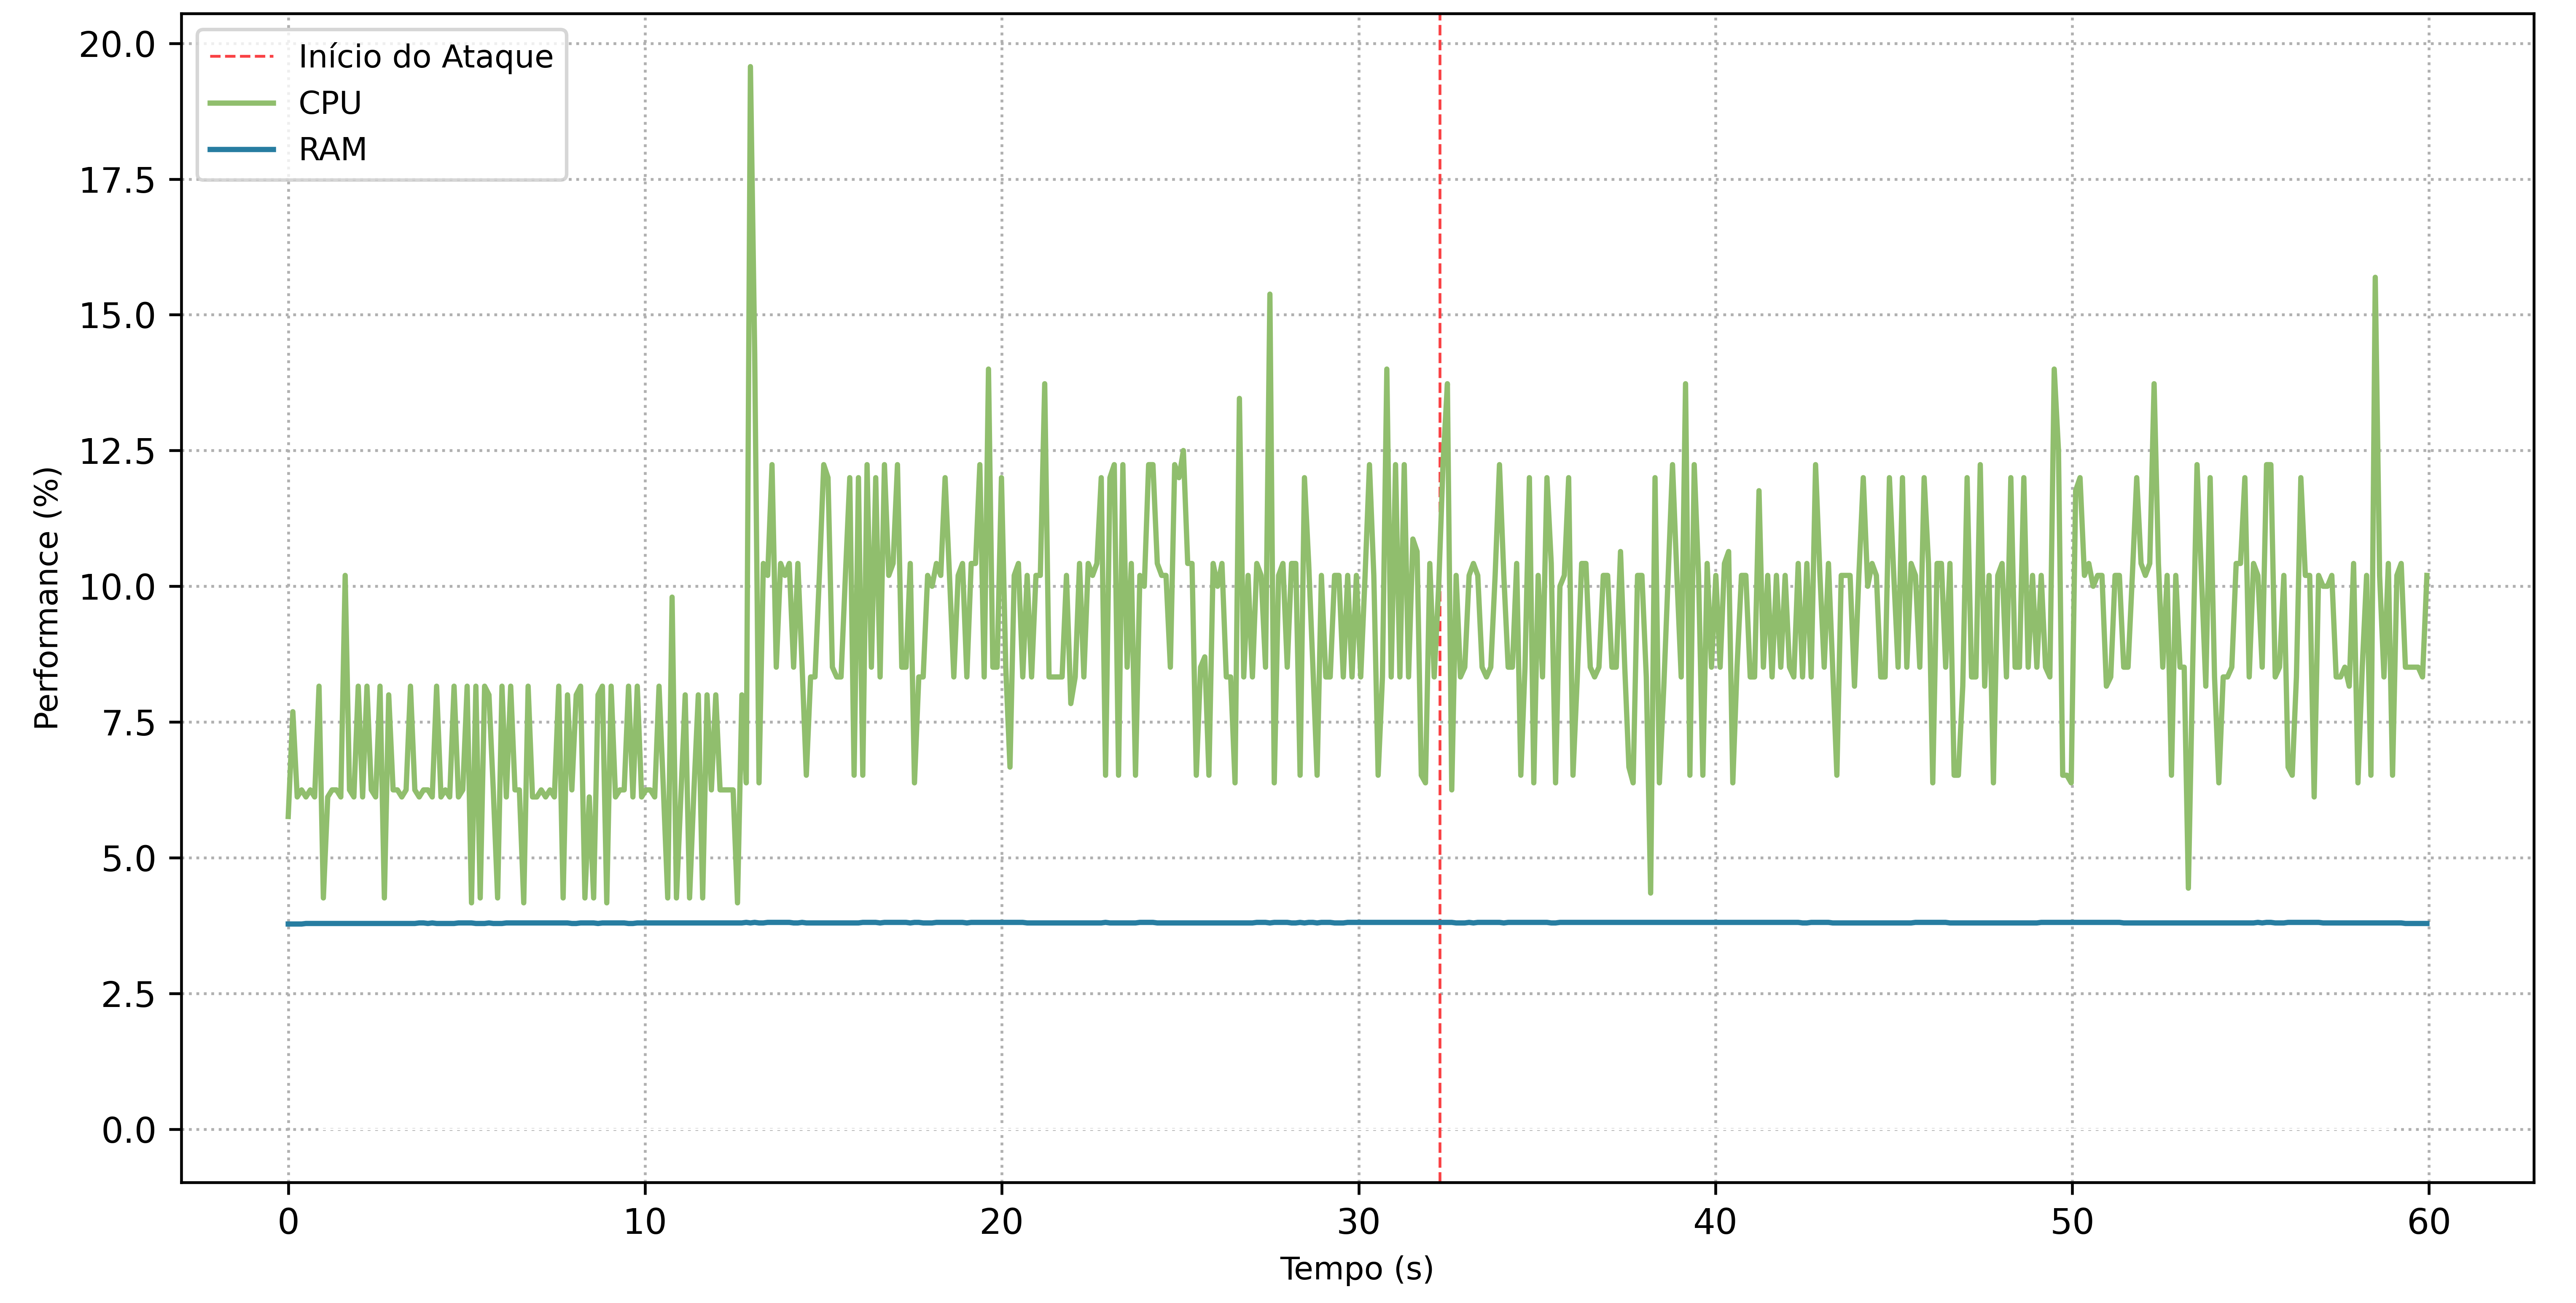
\includegraphics[width=1\textwidth, height=120pt]{USPSC-img/output/cropped/1-dos_certificate_inf_chain_loop-perf.png}
        \caption{Desempenho}
    \end{subfigure}%
    \\
    \begin{subfigure}[t]{0.5\textwidth}
        \centering
        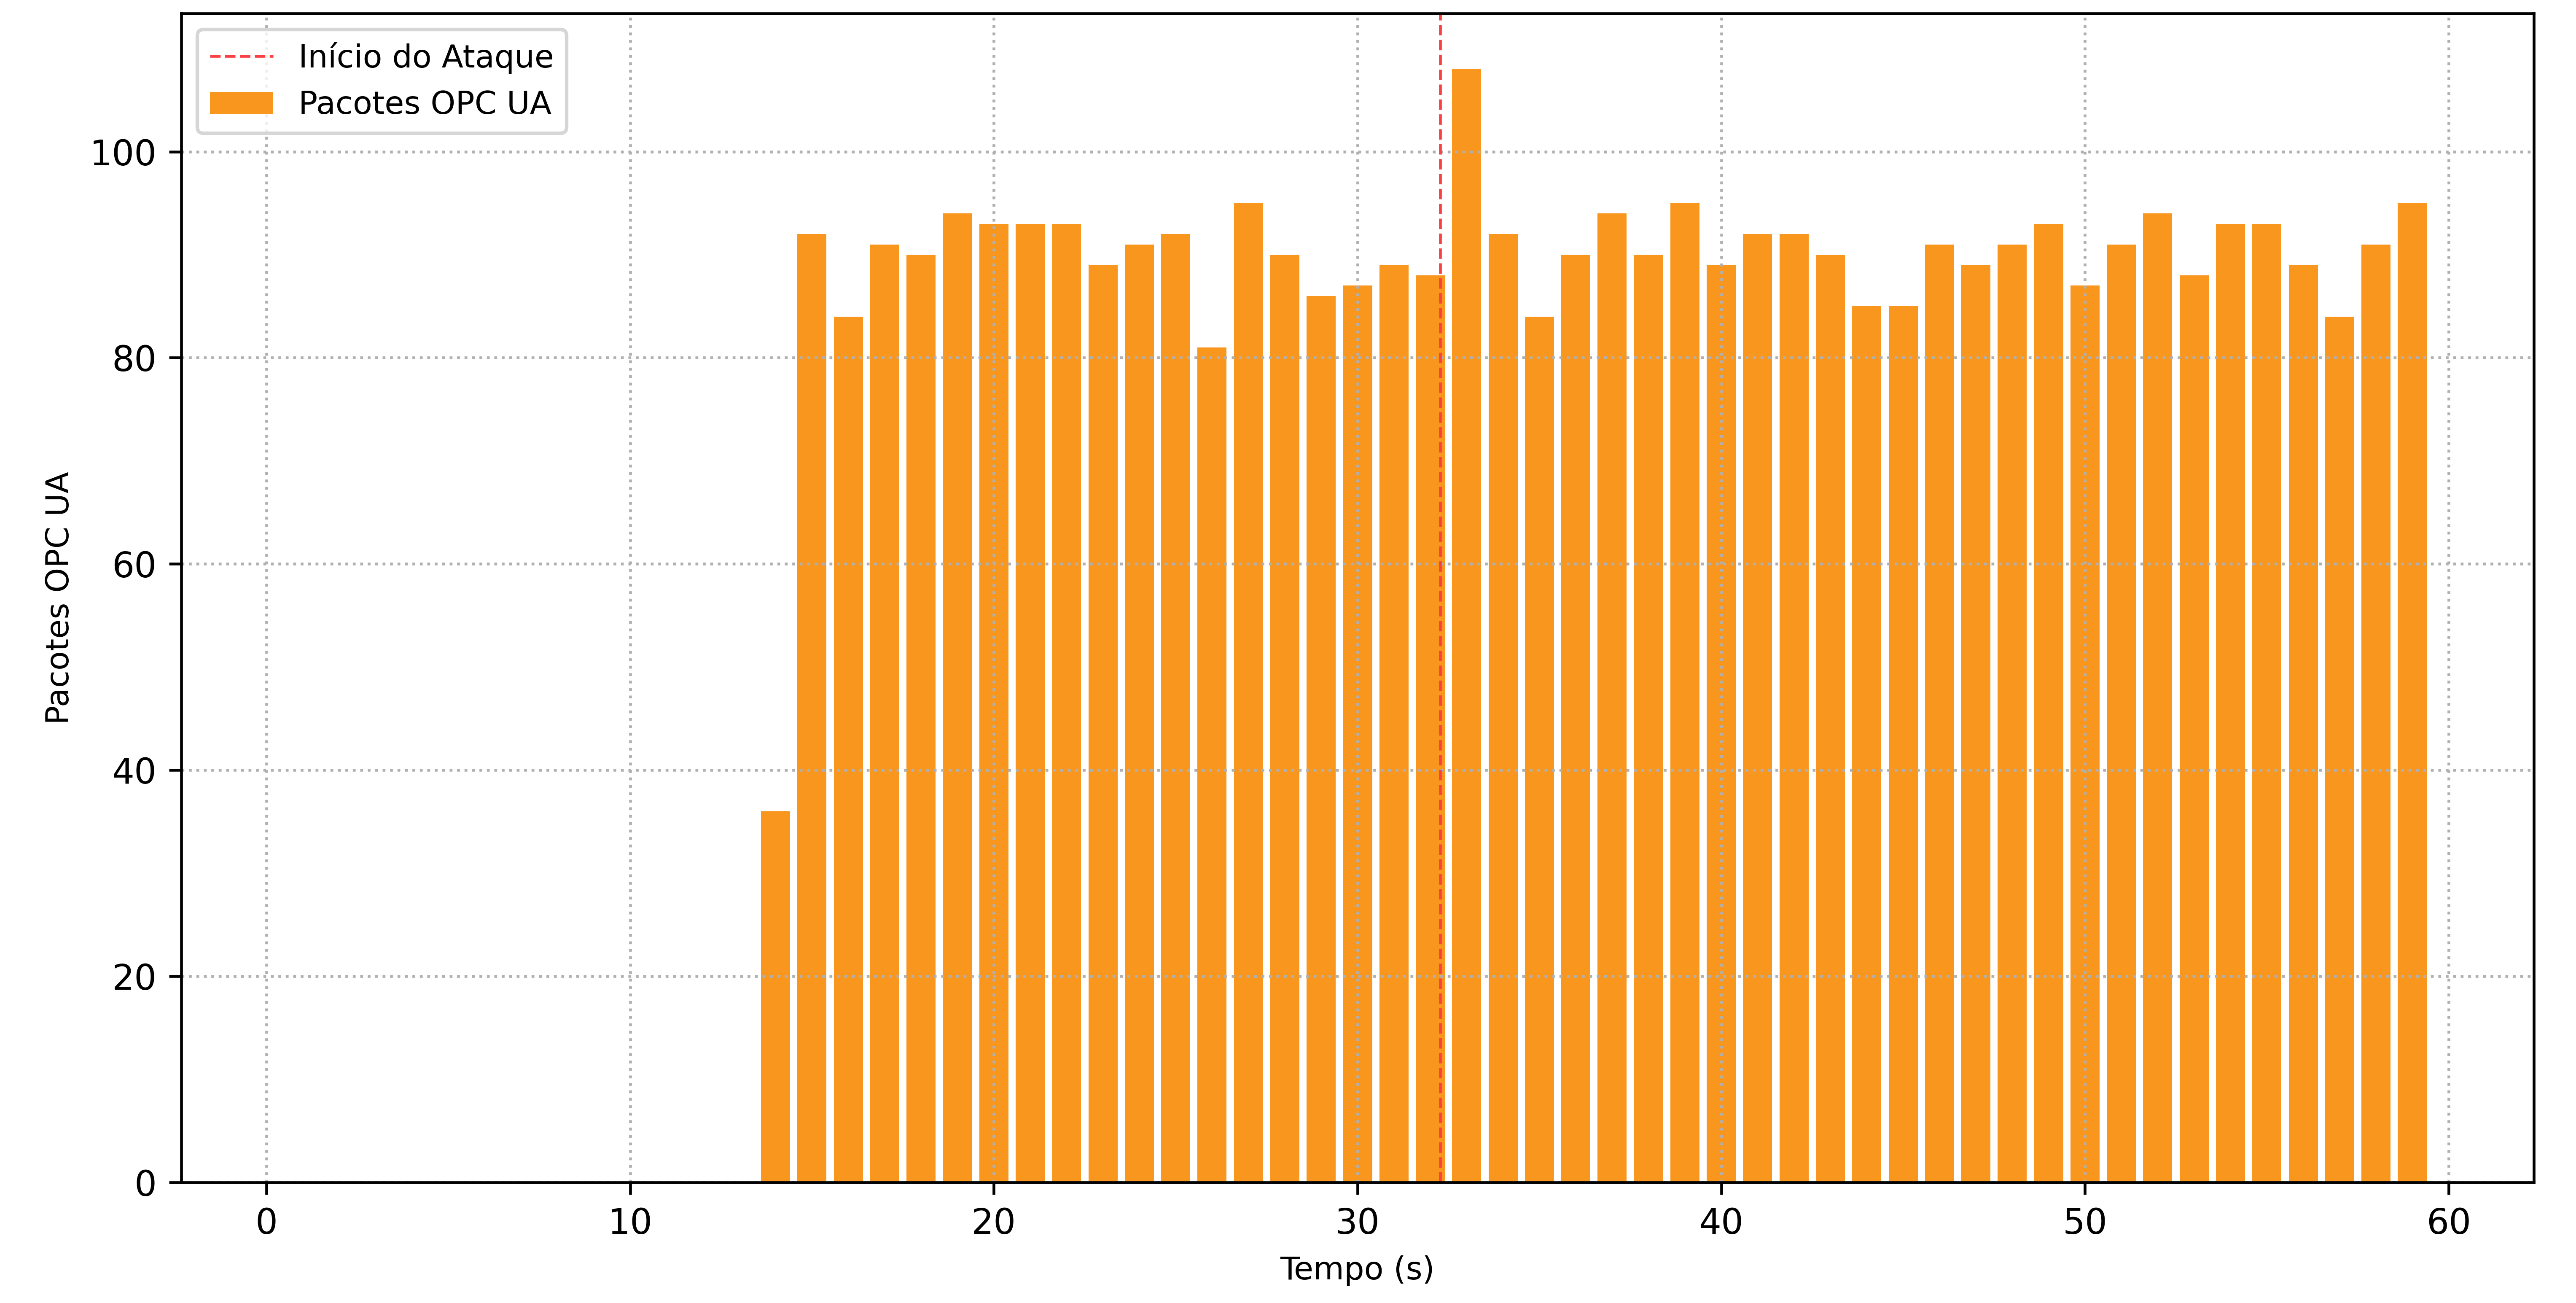
\includegraphics[width=1\textwidth, height=120pt]{USPSC-img/output/cropped/1-dos_certificate_inf_chain_loop-pack.png}
        \caption{Pacotes OPC UA}
    \end{subfigure}%
    ~
    \begin{subfigure}[t]{0.5\textwidth}
        \centering
        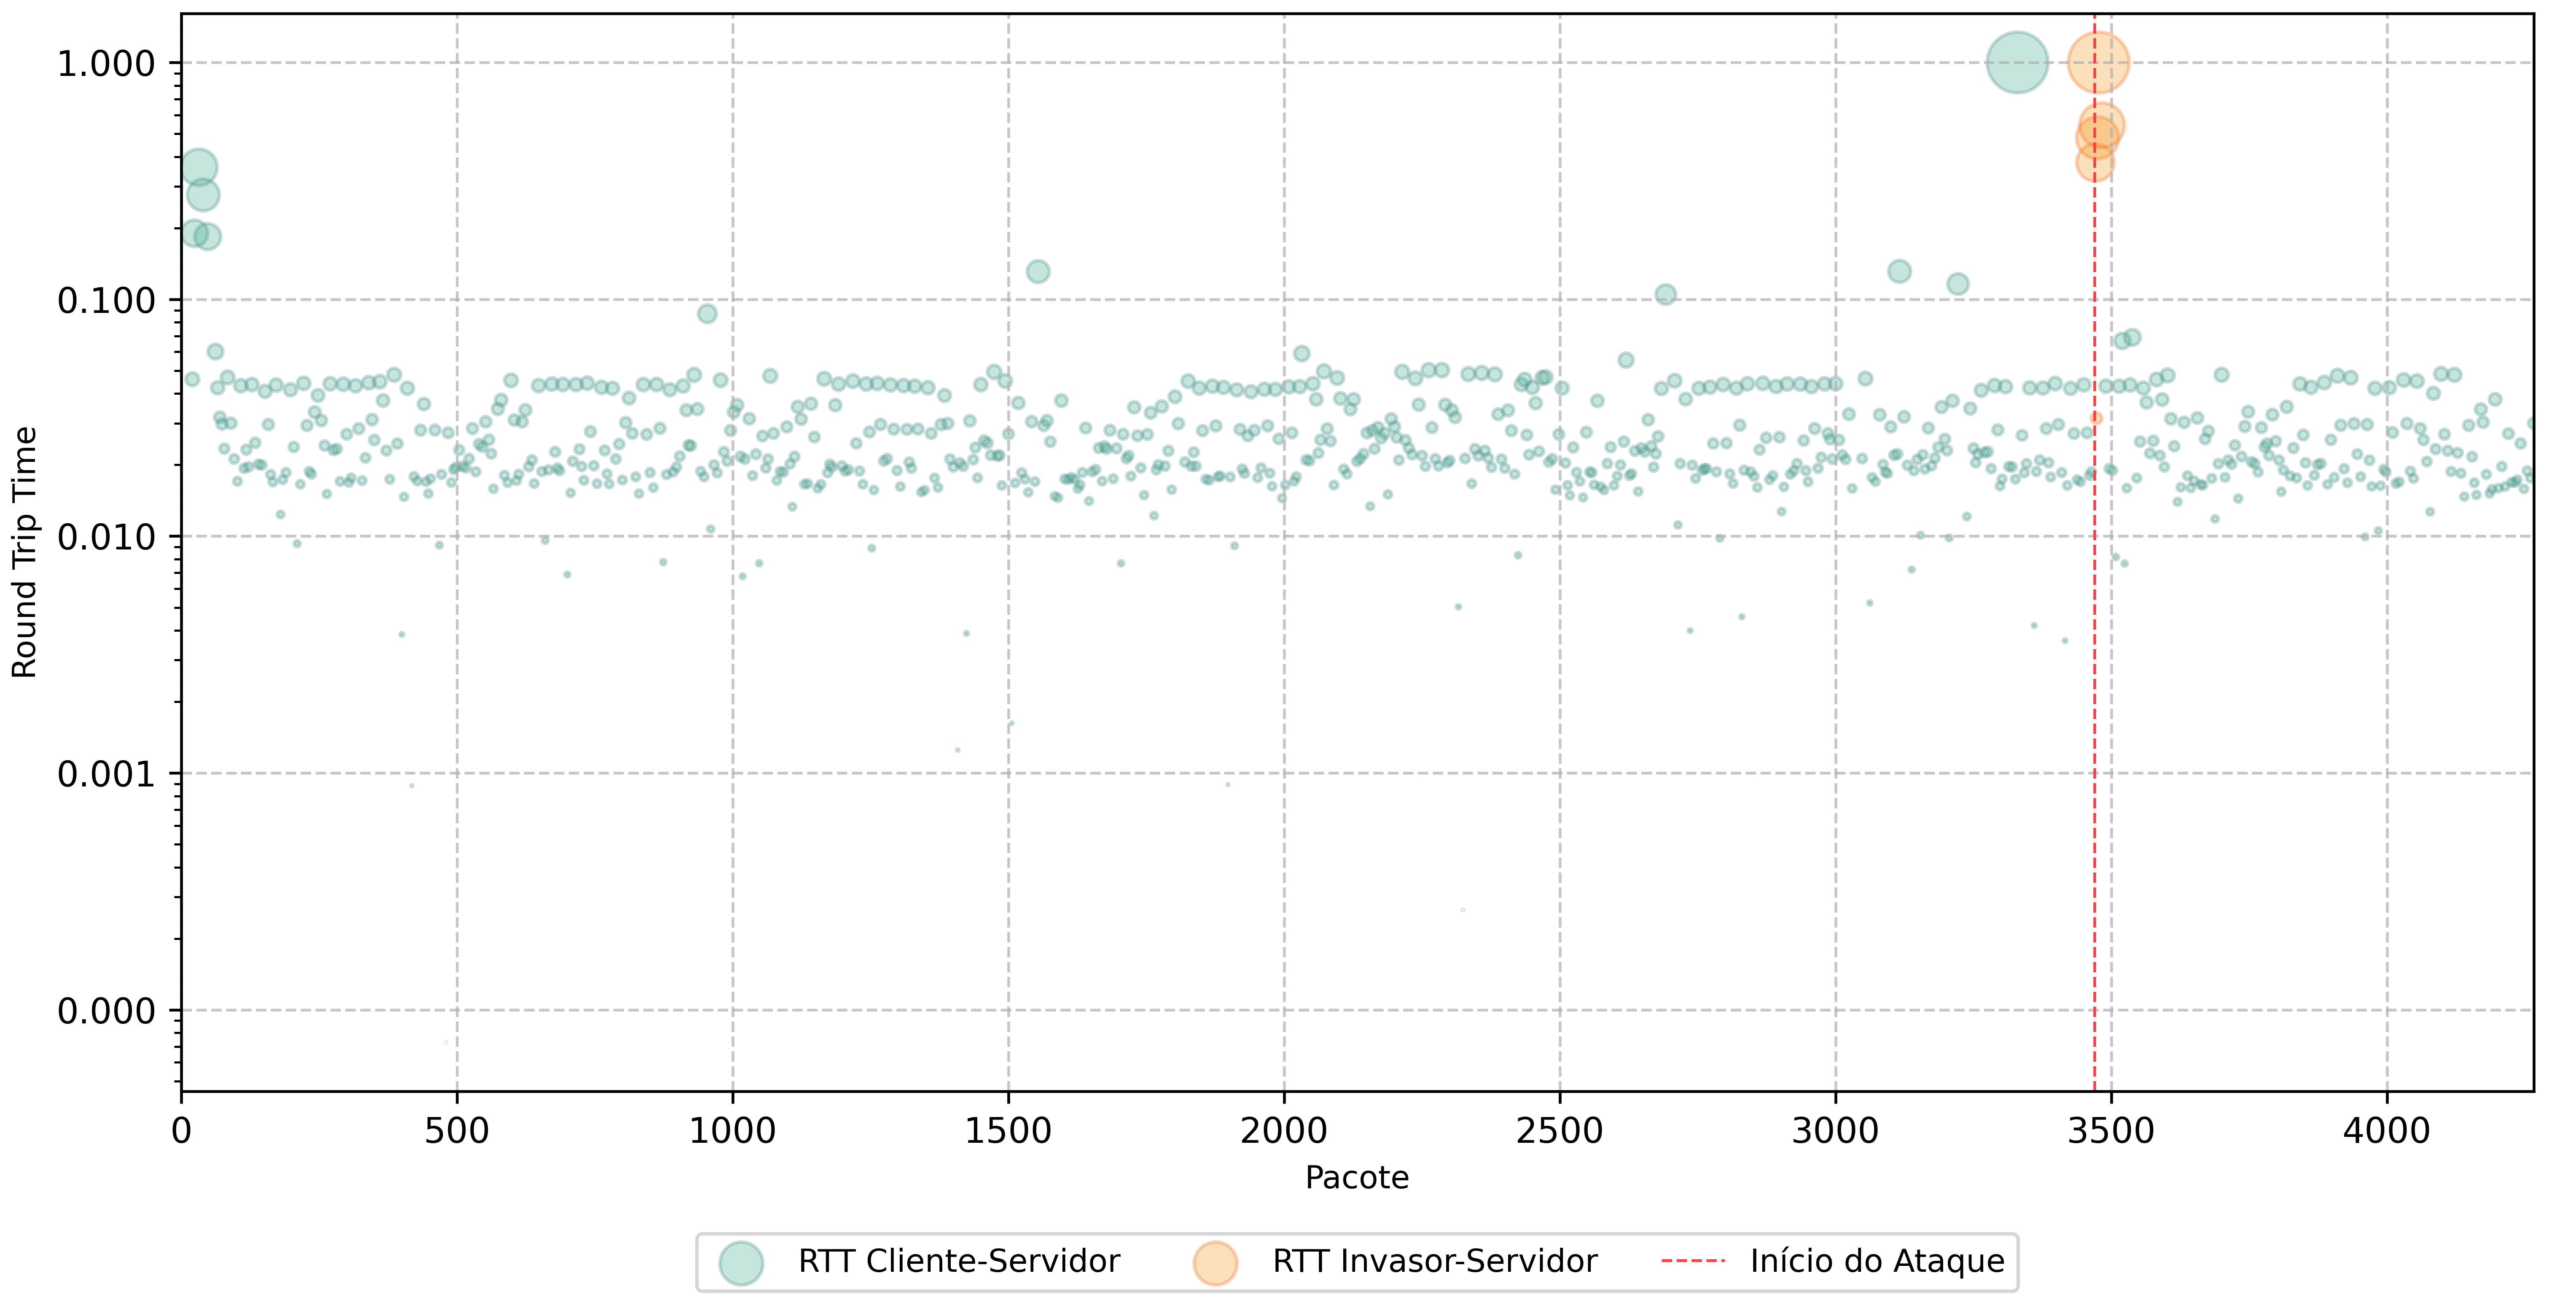
\includegraphics[width=1\textwidth, height=120pt]{USPSC-img/output/cropped/1-dos_certificate_inf_chain_loop-rttp.png}
        \caption{RTT por pacote}
    \end{subfigure}%
    % ~
    % \begin{subfigure}[t]{0.5\textwidth}
    %     \centering
    %     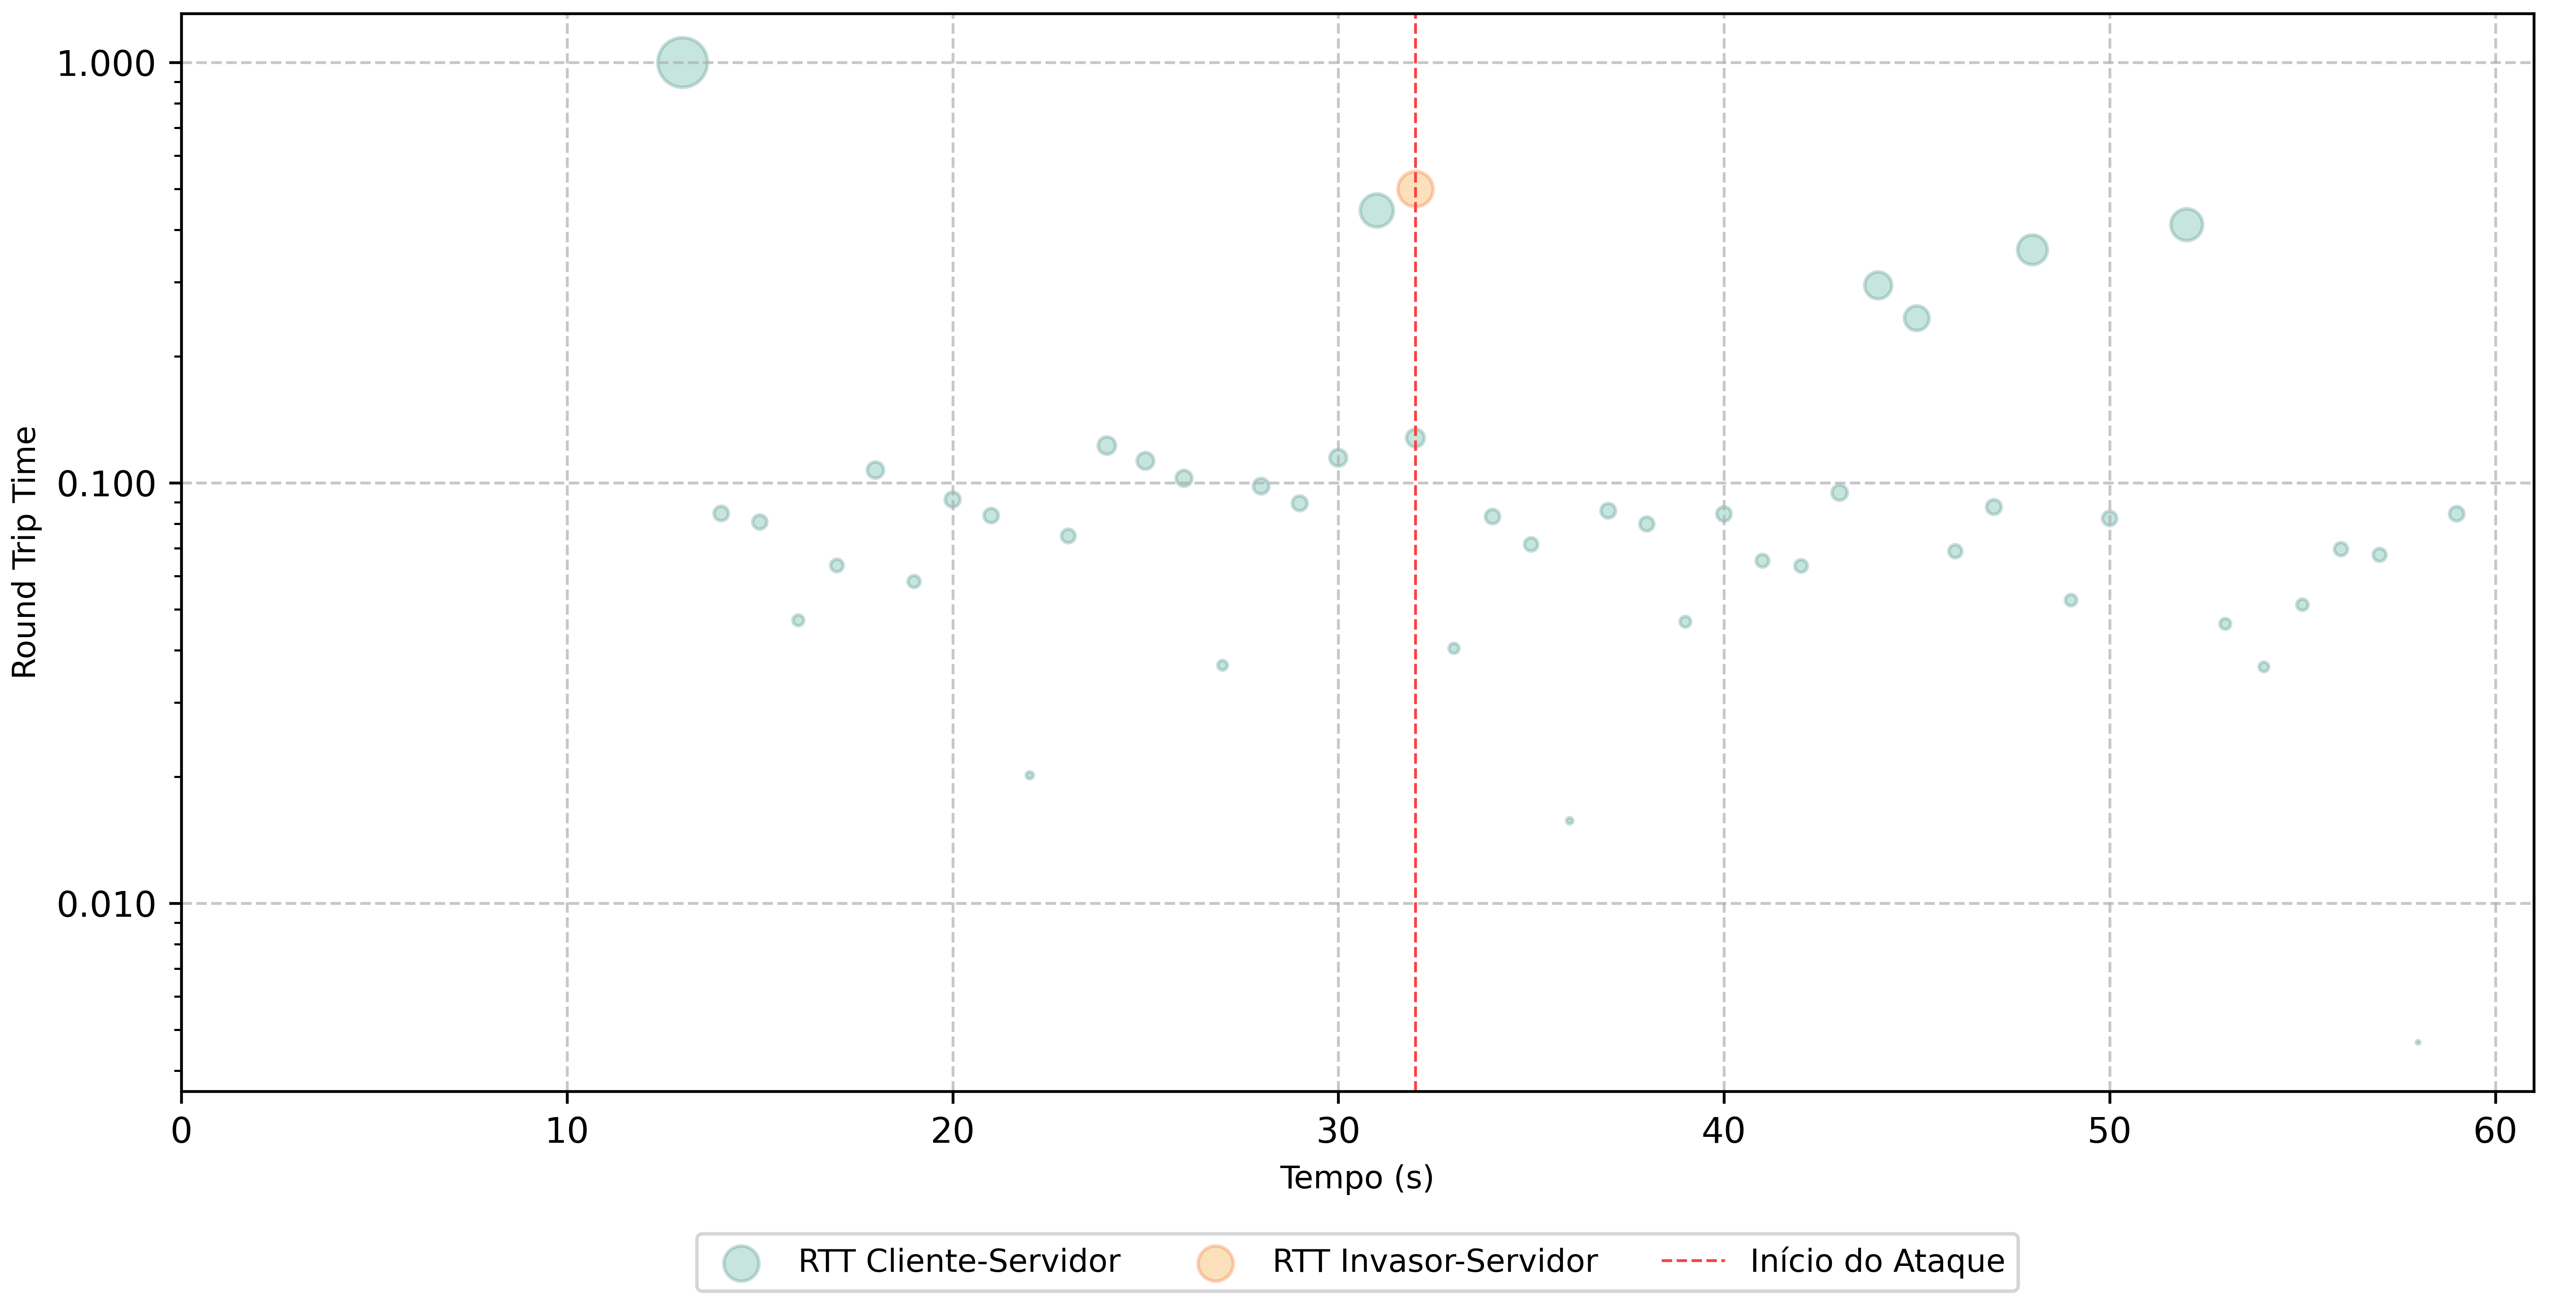
\includegraphics[width=1\textwidth, height=120pt]{USPSC-img/output/cropped/1-dos_certificate_inf_chain_loop-rtts.png}
    %     \caption{RTT por segundos}
    % \end{subfigure}%
    \label{fig:1-dos_certificate_inf_chain_loop}
    \caption{Gráficos do ataque de DoS por loop infinito na cadeia de certificados - nível de segurança: `Sign'.}
\end{figure}

\begin{figure}[htbp!]
    \centering
    \begin{subfigure}[t]{0.5\textwidth}
        \centering
        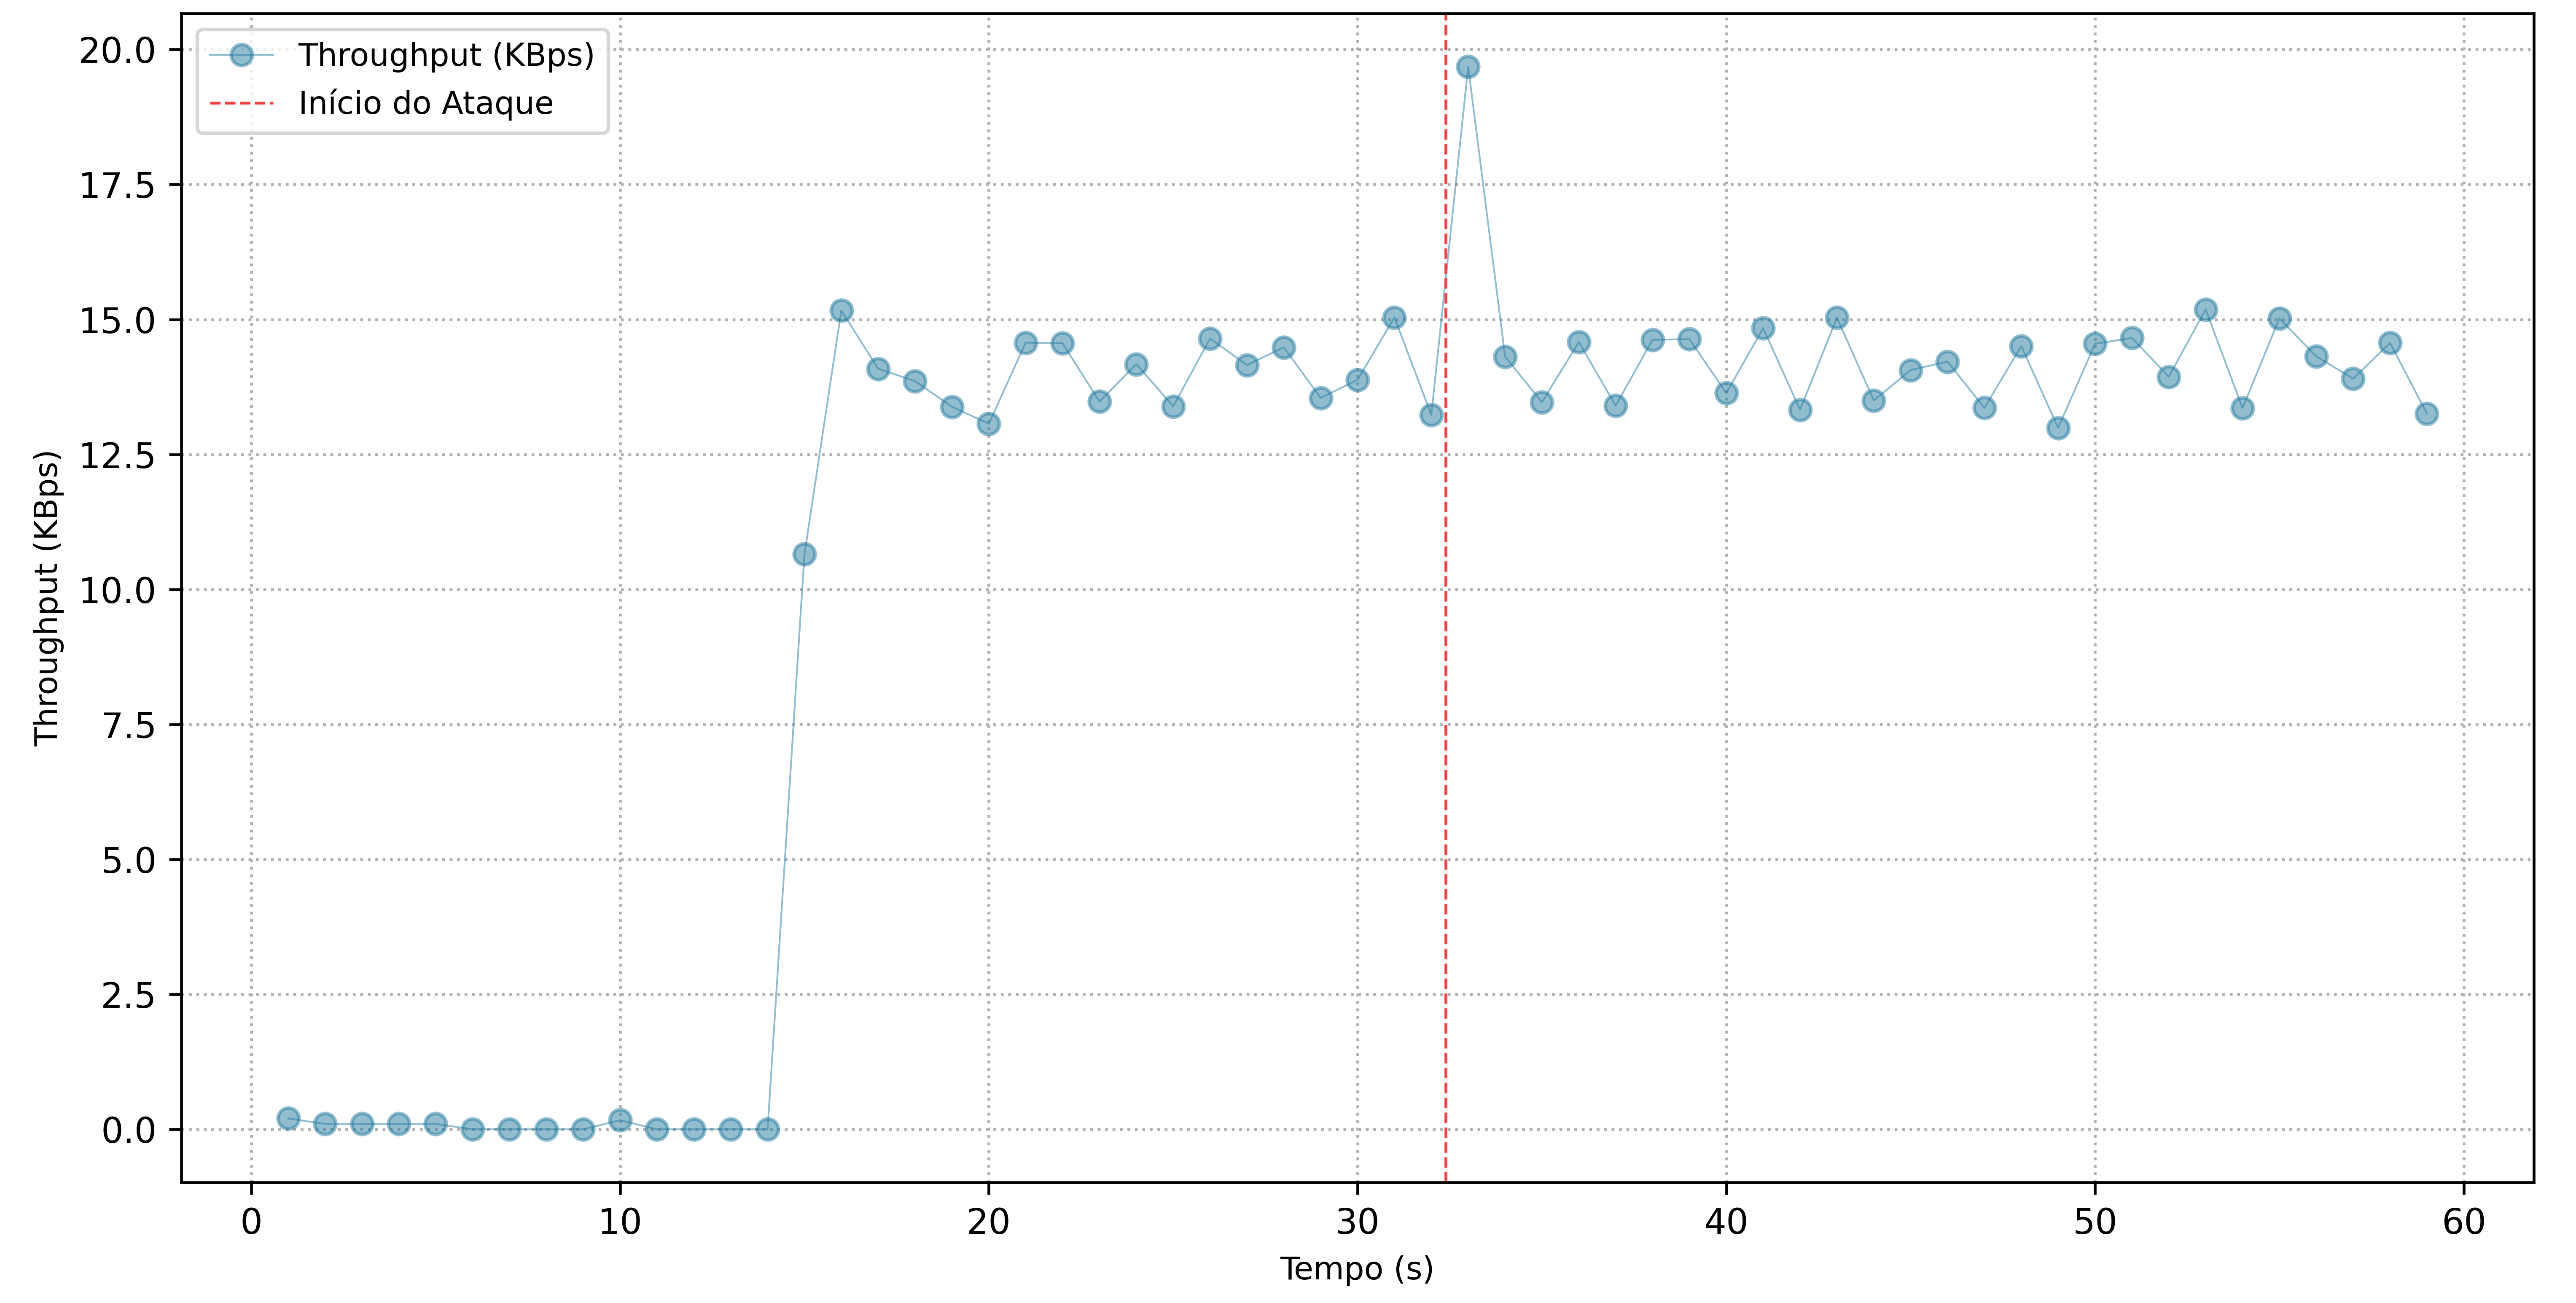
\includegraphics[width=1\textwidth, height=120pt]{USPSC-img/output/cropped/2-dos_certificate_inf_chain_loop-tput.png}
        \caption{\textit{Throughput}}
    \end{subfigure}%
    ~ 
    \begin{subfigure}[t]{0.5\textwidth}
        \centering
        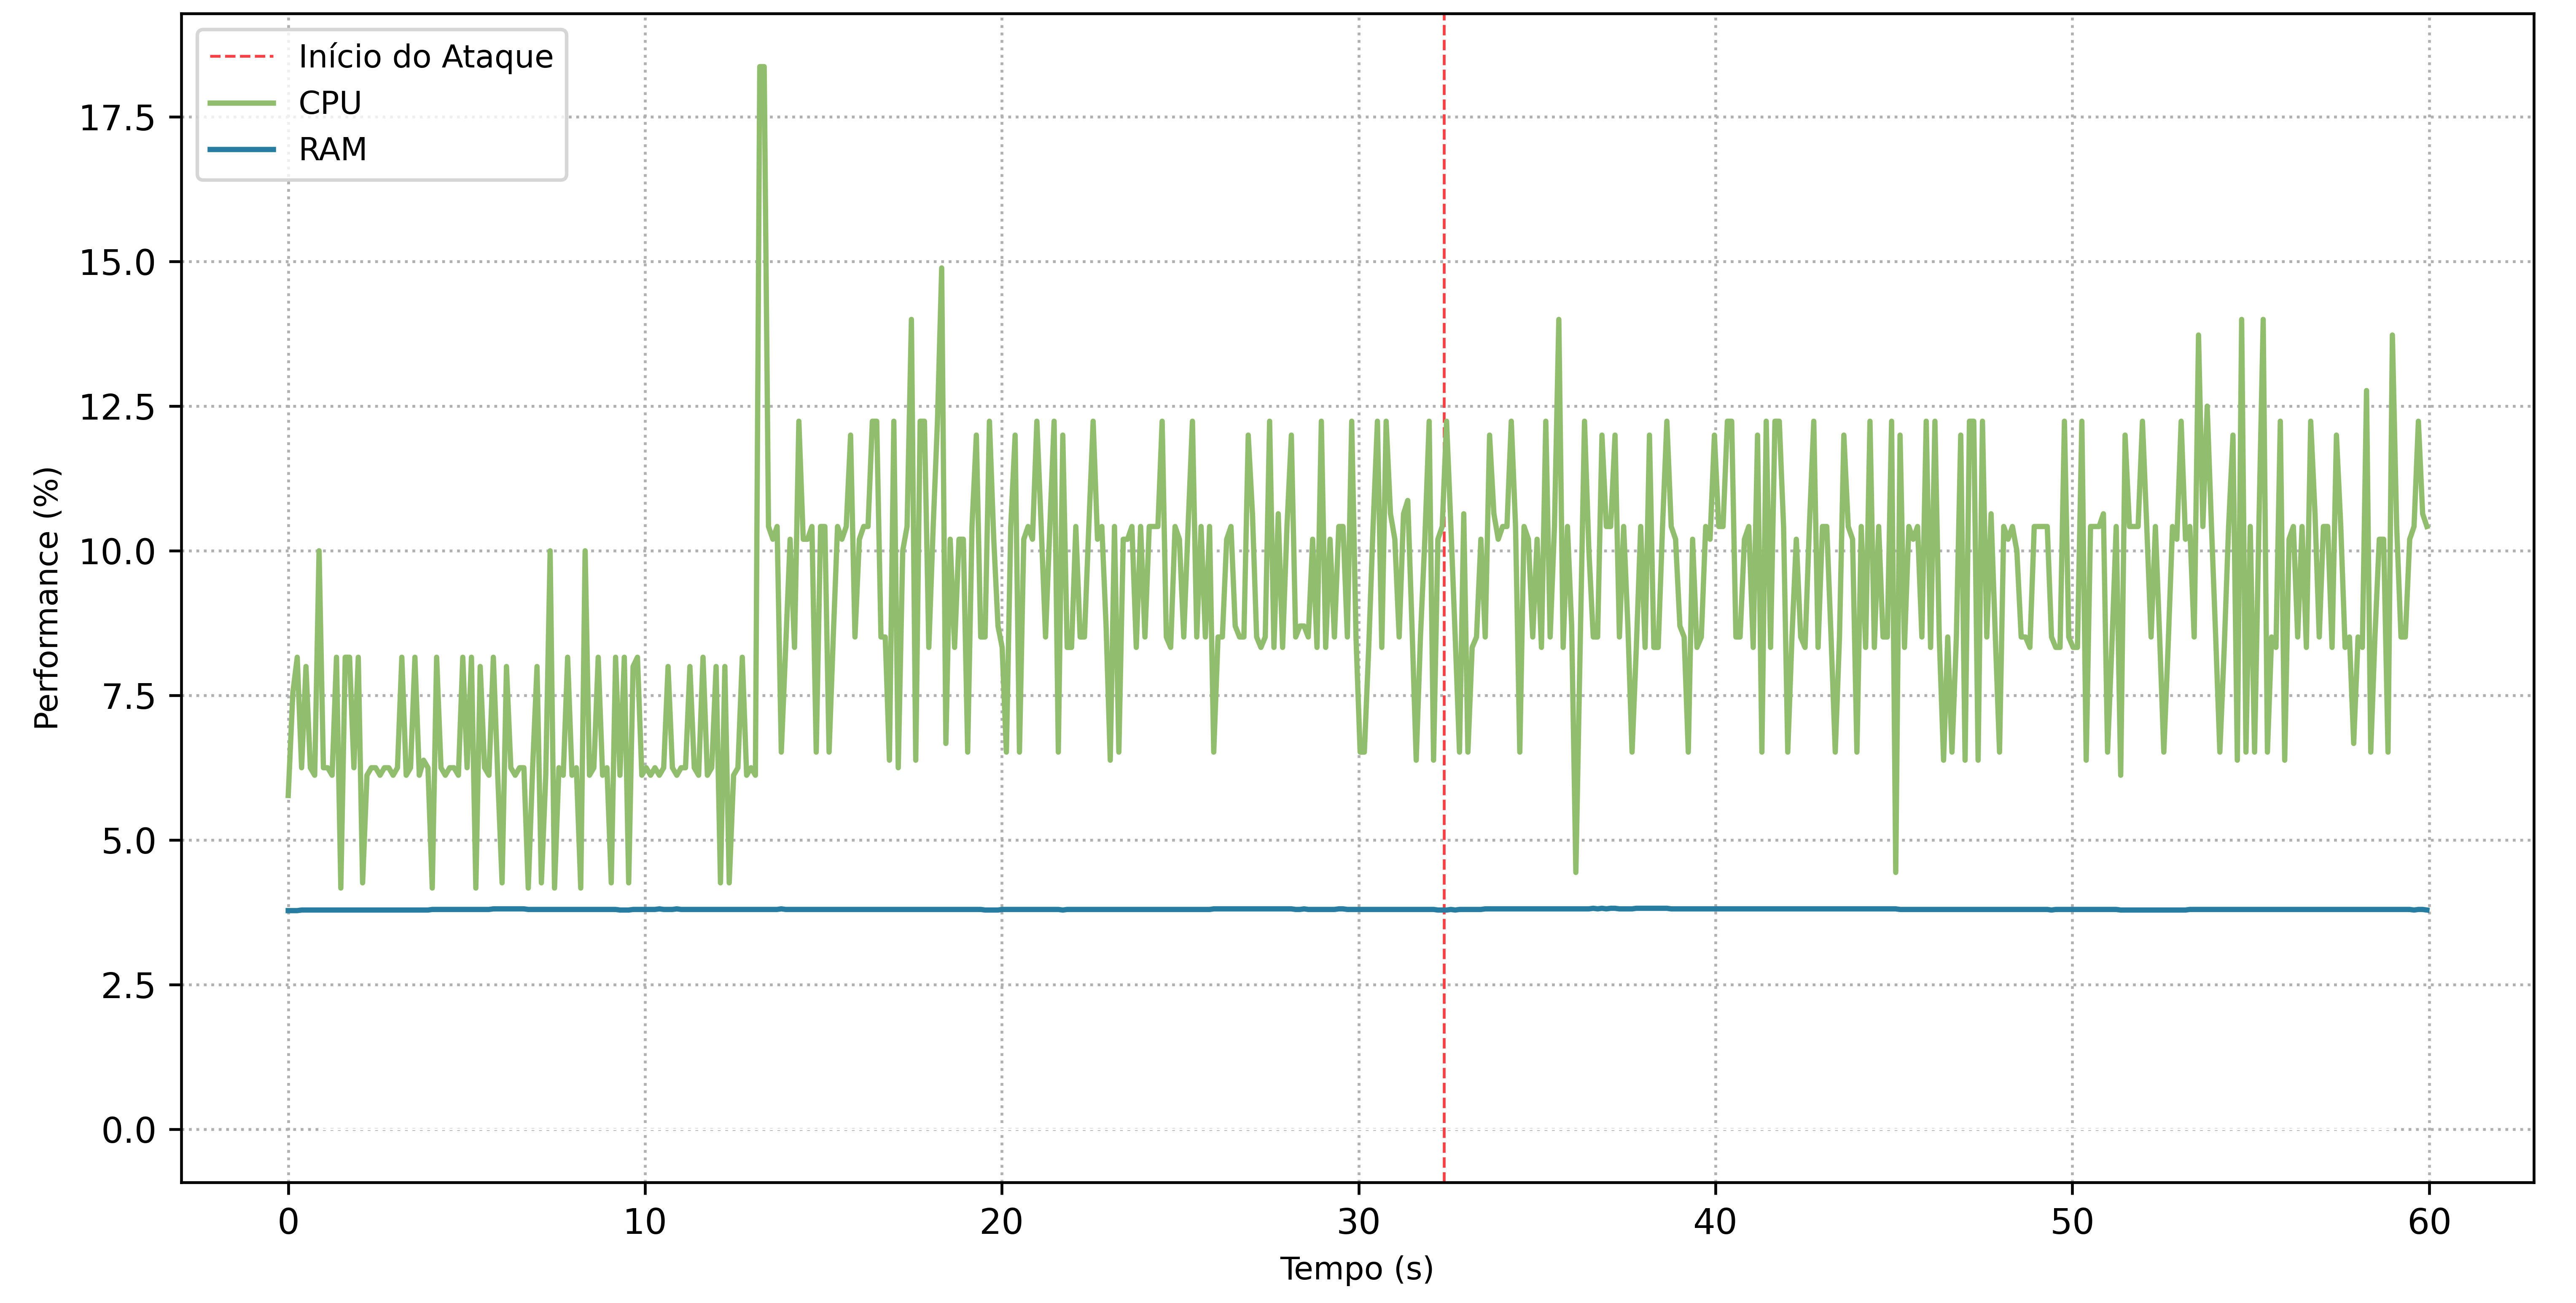
\includegraphics[width=1\textwidth, height=120pt]{USPSC-img/output/cropped/2-dos_certificate_inf_chain_loop-perf.png}
        \caption{Desempenho}
    \end{subfigure}%
    \\
    \begin{subfigure}[t]{0.5\textwidth}
        \centering
        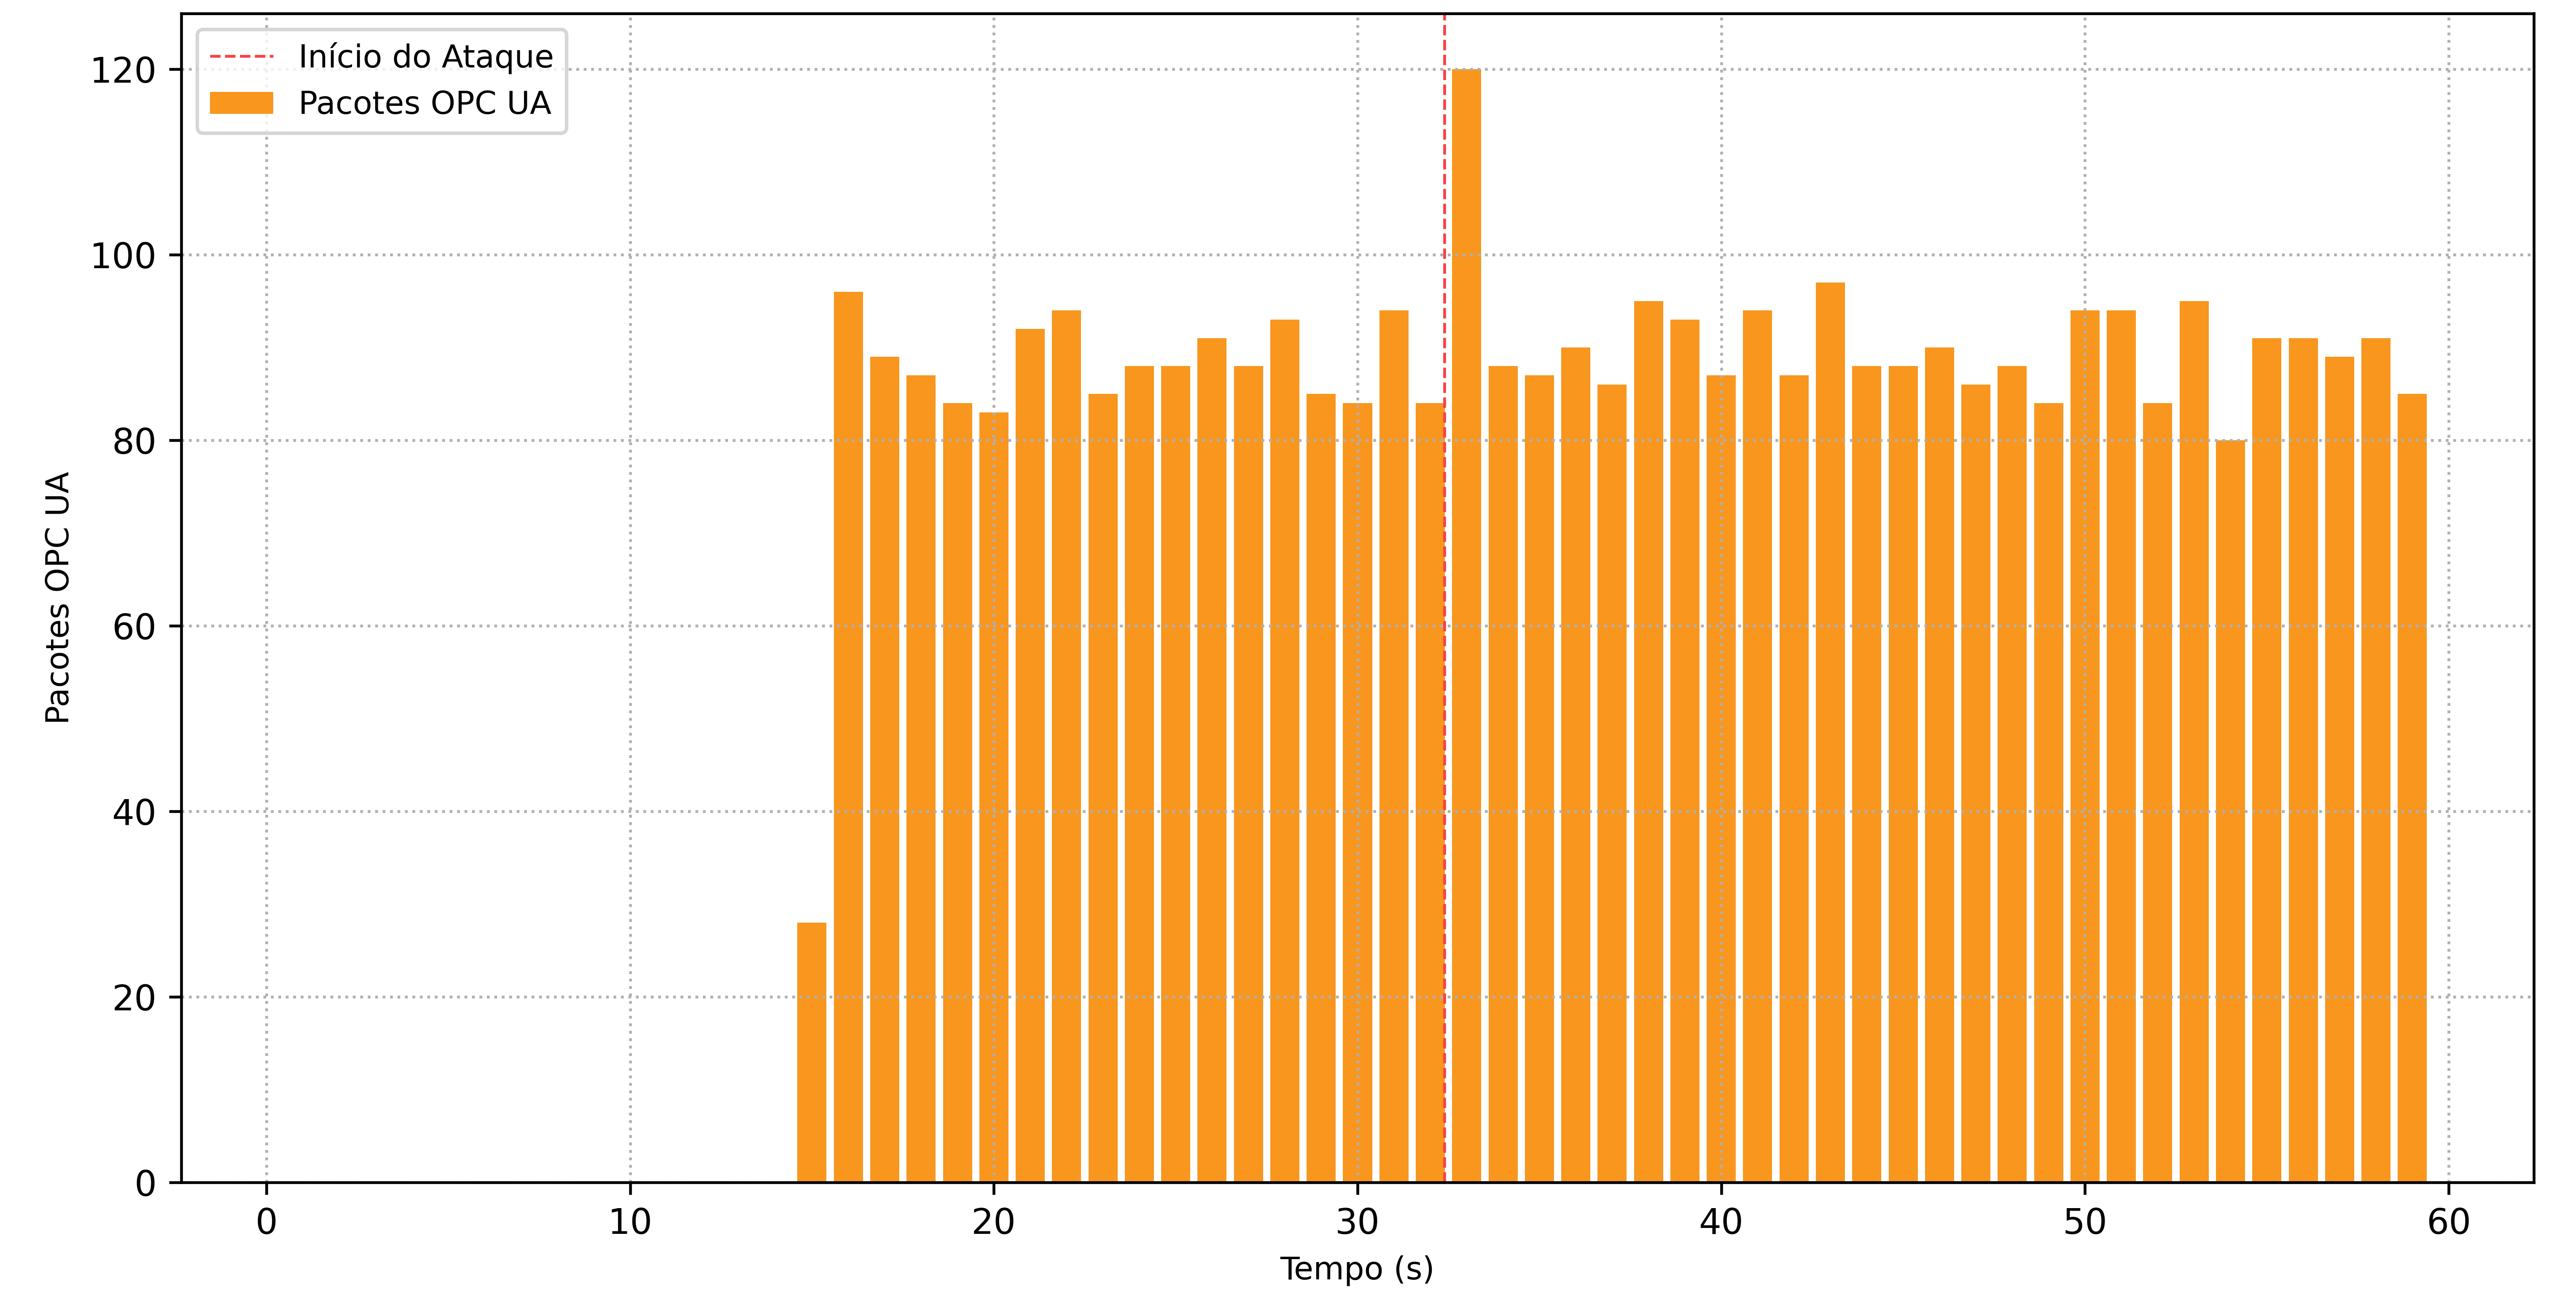
\includegraphics[width=1\textwidth, height=120pt]{USPSC-img/output/cropped/2-dos_certificate_inf_chain_loop-pack.png}
        \caption{Pacotes OPC UA}
    \end{subfigure}%
    ~
    \begin{subfigure}[t]{0.5\textwidth}
        \centering
        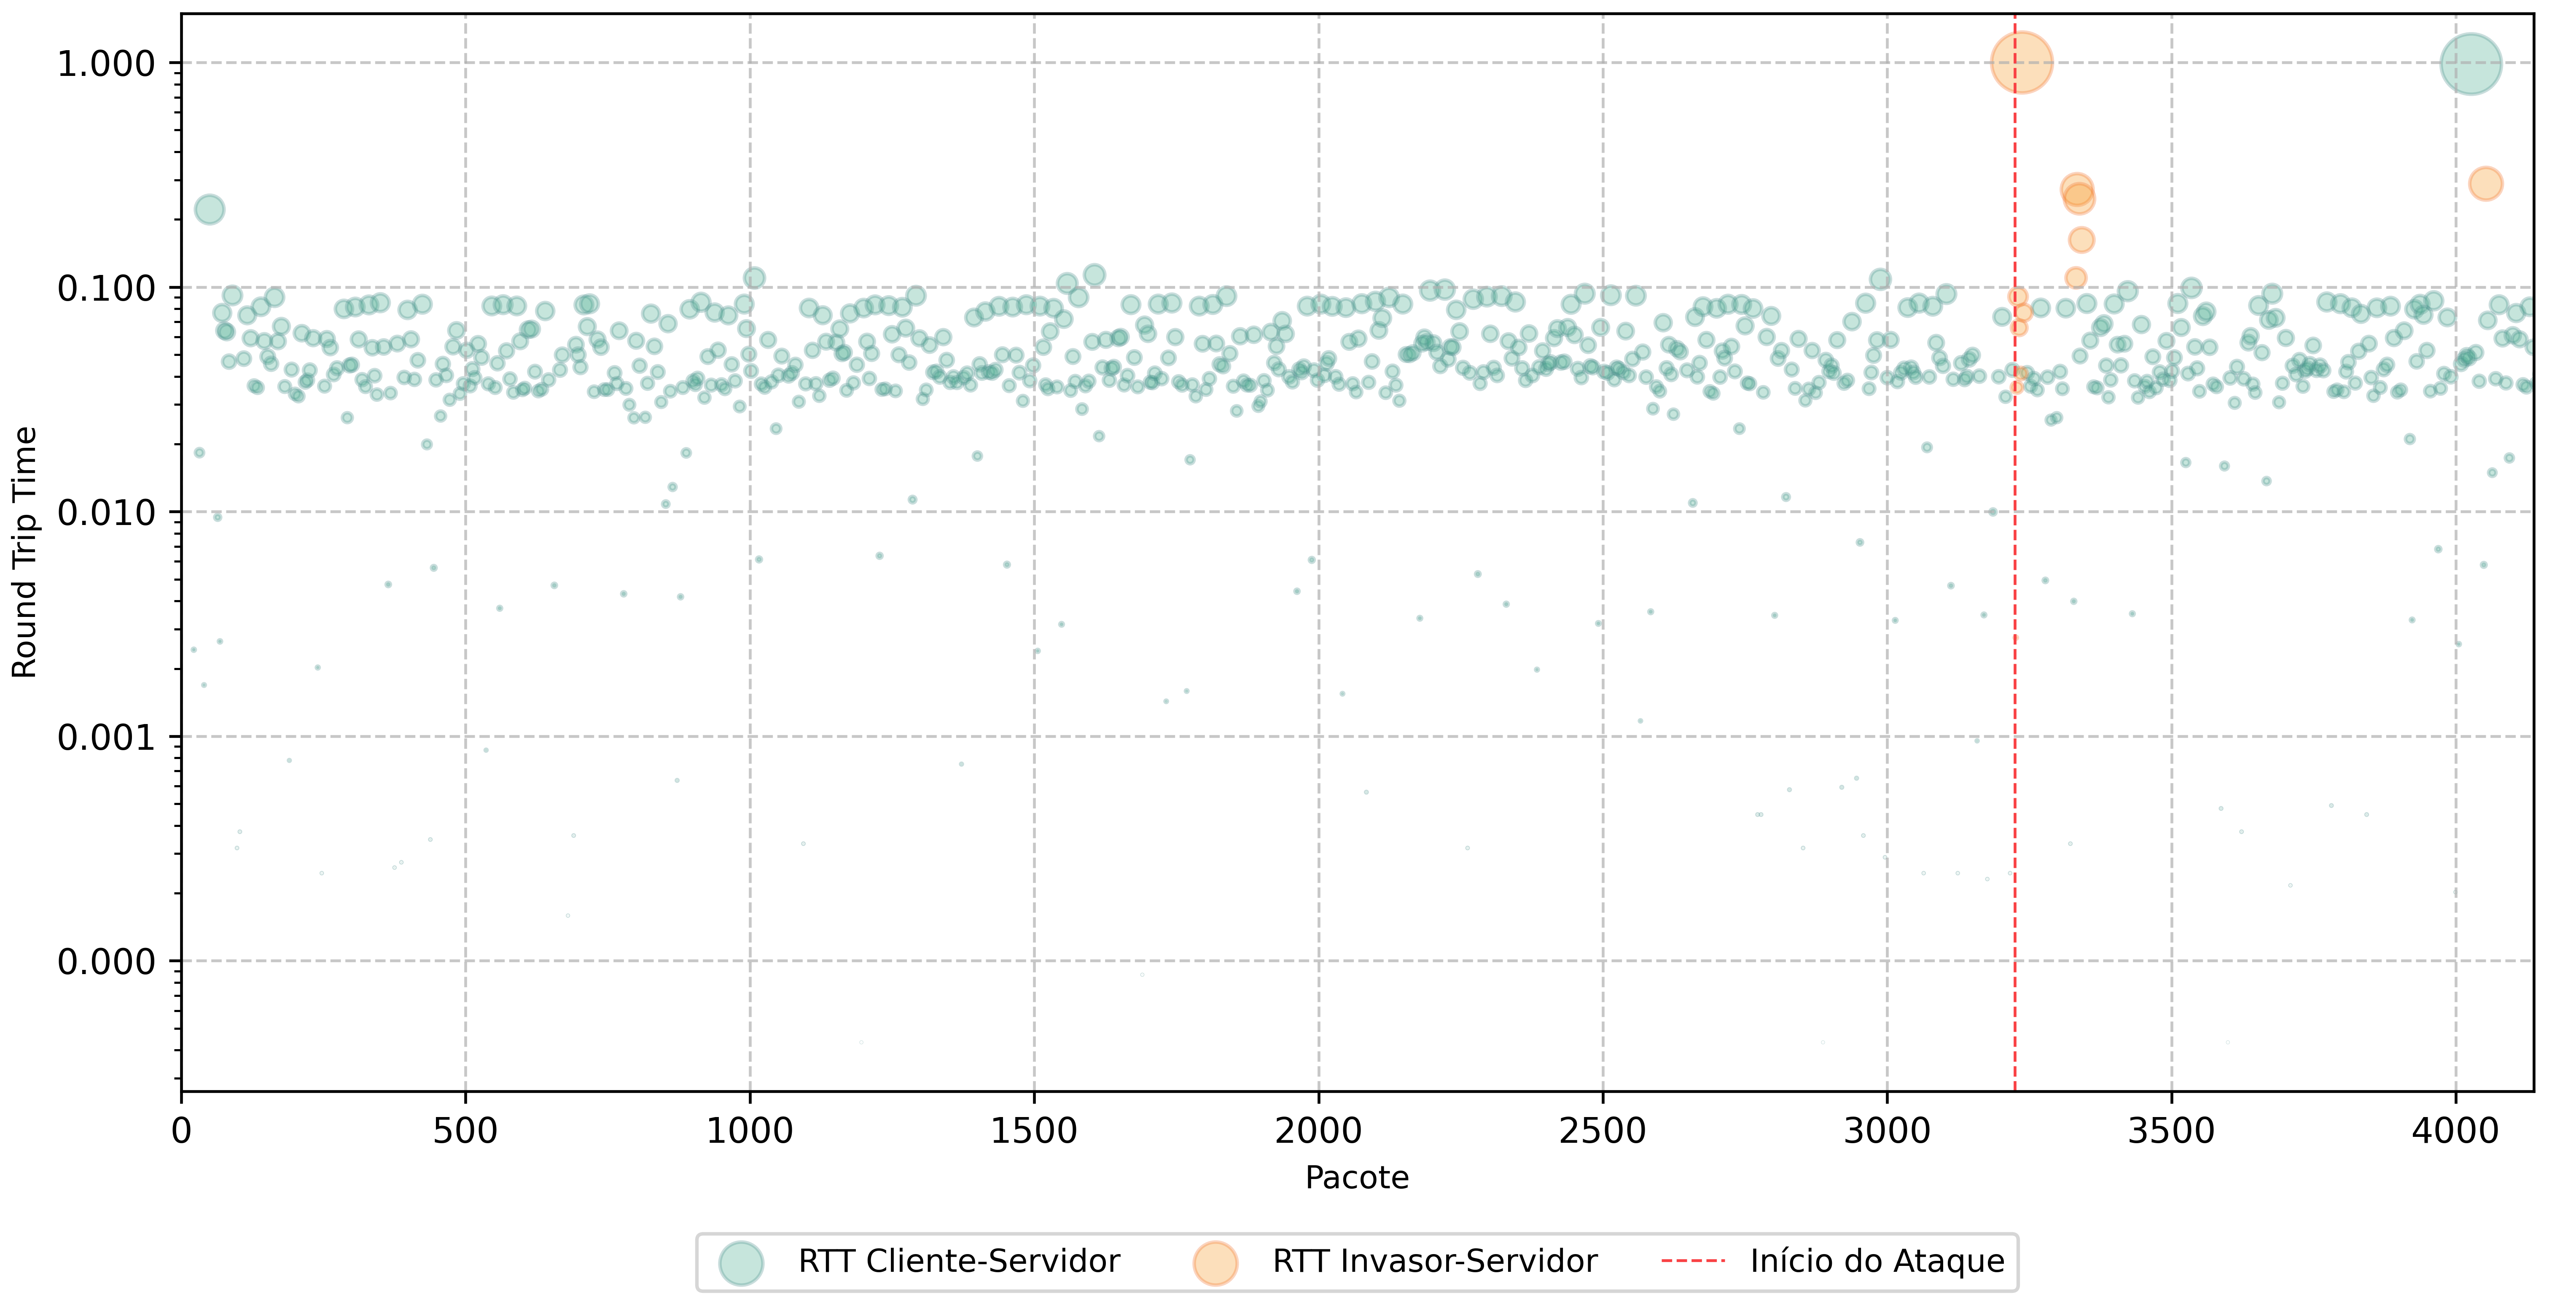
\includegraphics[width=1\textwidth, height=120pt]{USPSC-img/output/cropped/2-dos_certificate_inf_chain_loop-rttp.png}
        \caption{RTT por pacote}
    \end{subfigure}%
    % ~
    % \begin{subfigure}[t]{0.5\textwidth}
    %     \centering
    %     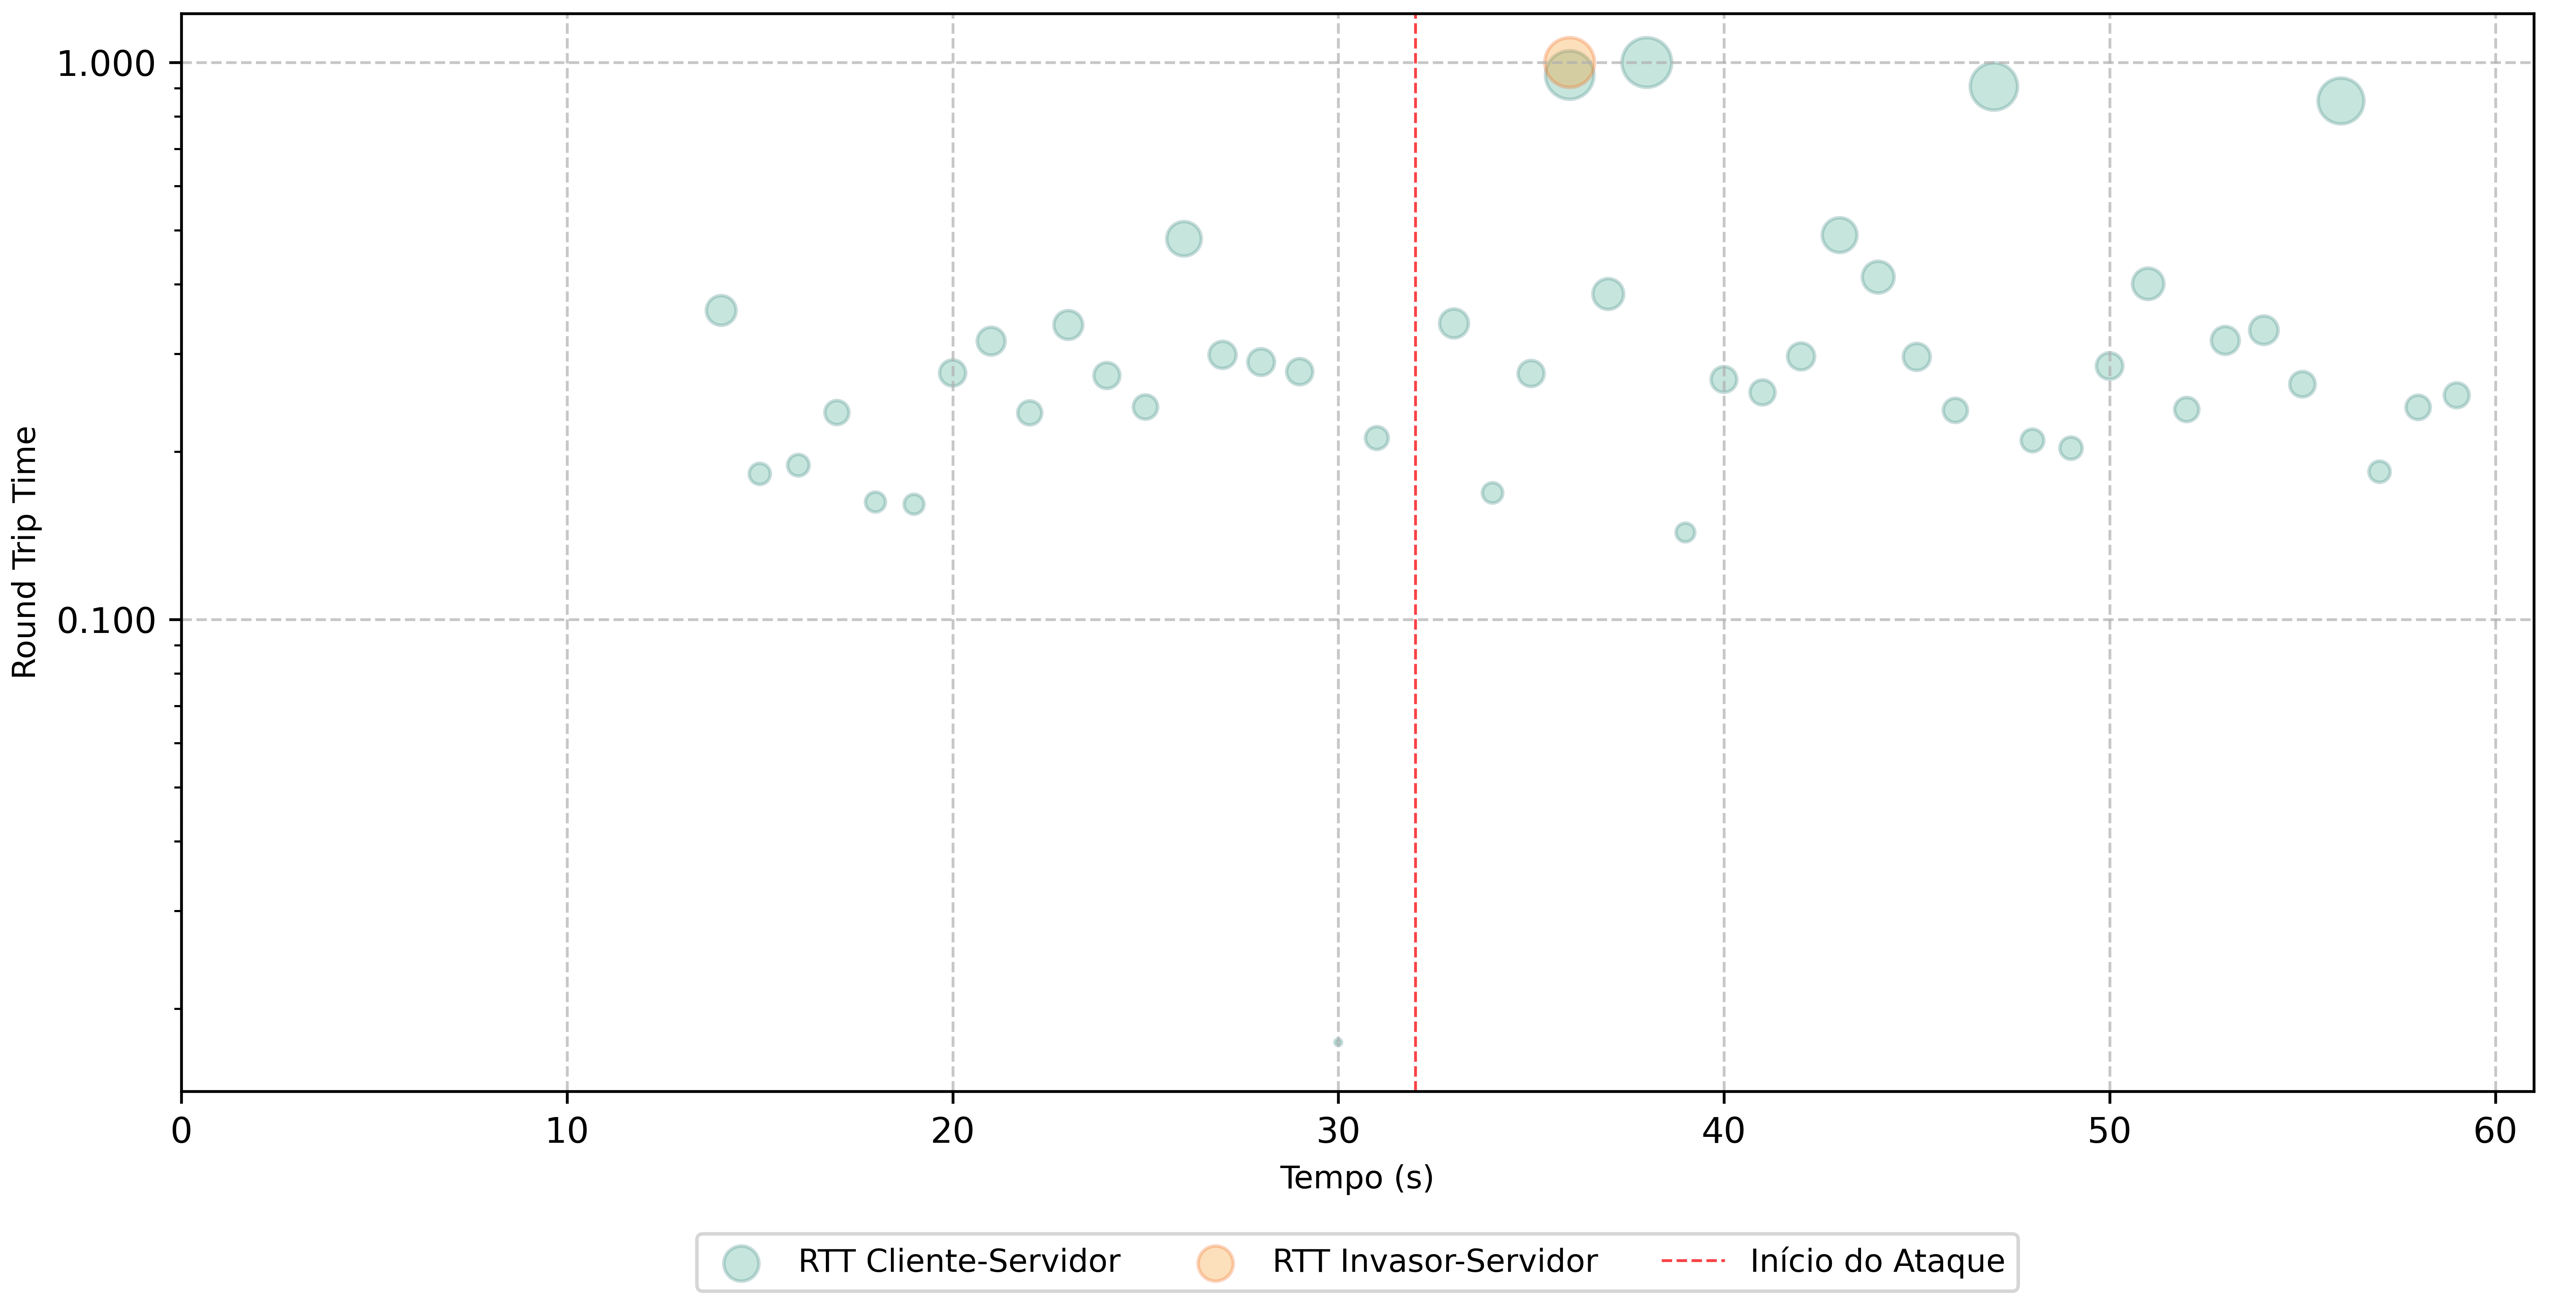
\includegraphics[width=1\textwidth, height=120pt]{USPSC-img/output/cropped/2-dos_certificate_inf_chain_loop-rtts.png}
    %     \caption{RTT por segundos}
    % \end{subfigure}%
    \label{fig:2-dos_certificate_inf_chain_loop}
    \caption{Gráficos do ataque de DoS por loop infinito na cadeia de certificados - nível de segurança: `Sign \& Encrypt'.}
\end{figure}

\begin{figure}[htbp!]
    \centering
    \begin{subfigure}[t]{0.5\textwidth}
        \centering
        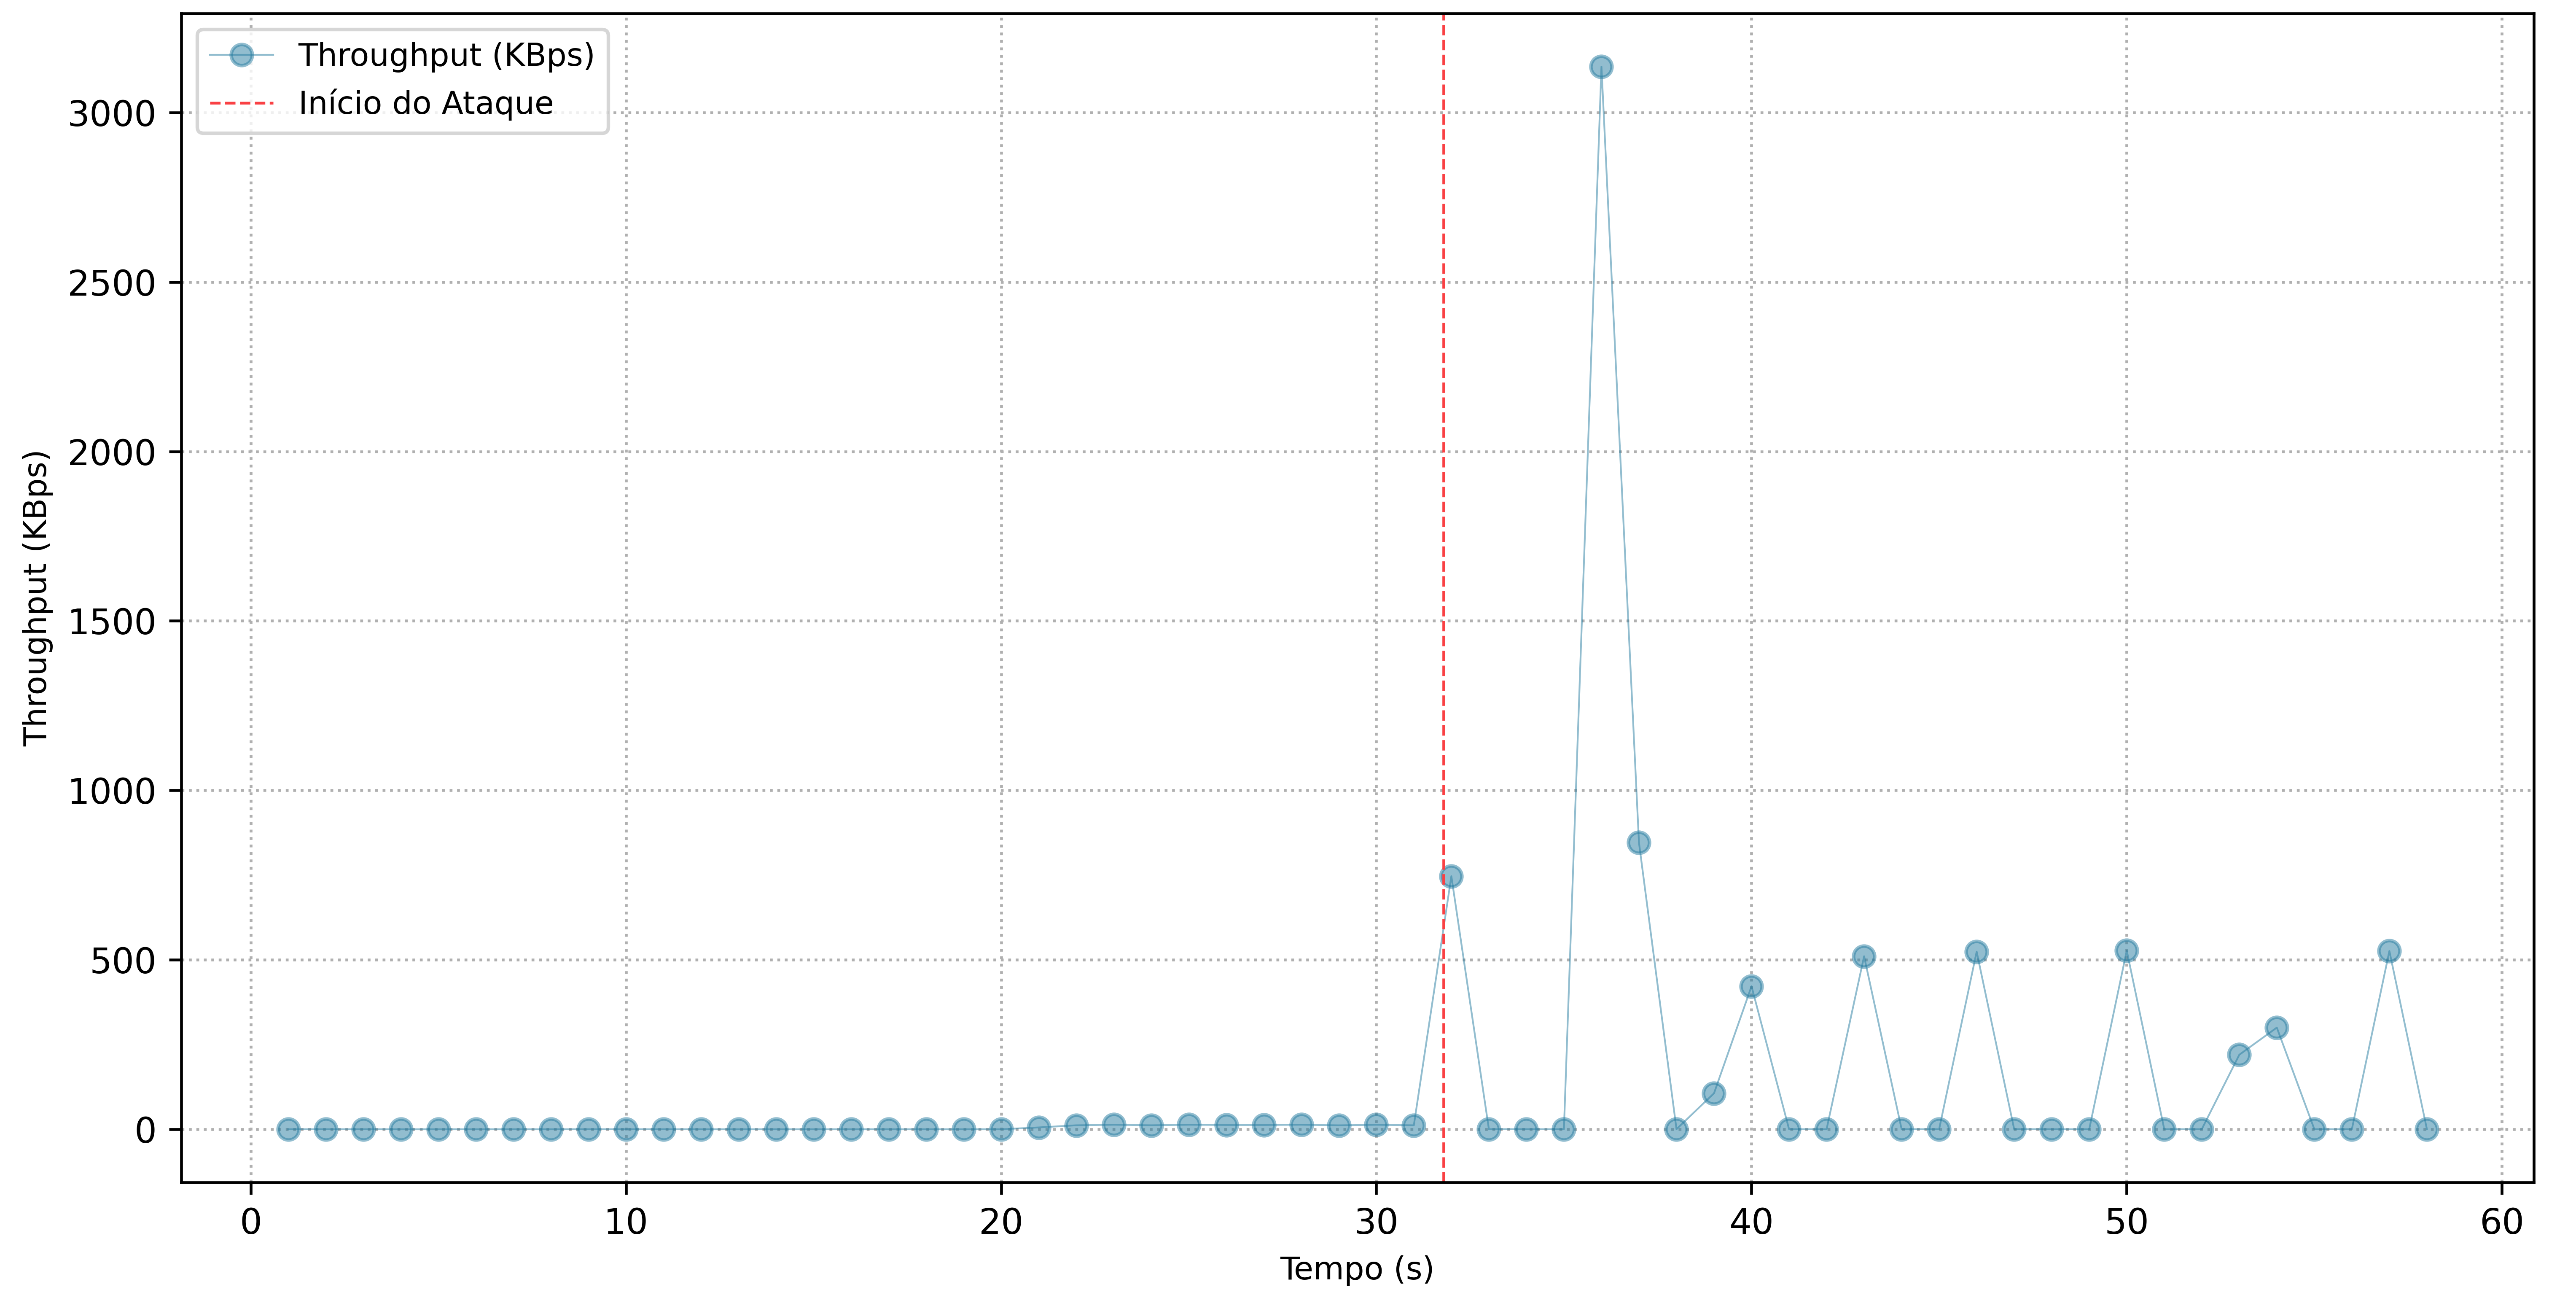
\includegraphics[width=1\textwidth, height=120pt]{USPSC-img/output/cropped/0-dos_function_call_null_deref-tput.png}
        \caption{\textit{Throughput}}
    \end{subfigure}%
    ~ 
    \begin{subfigure}[t]{0.5\textwidth}
        \centering
        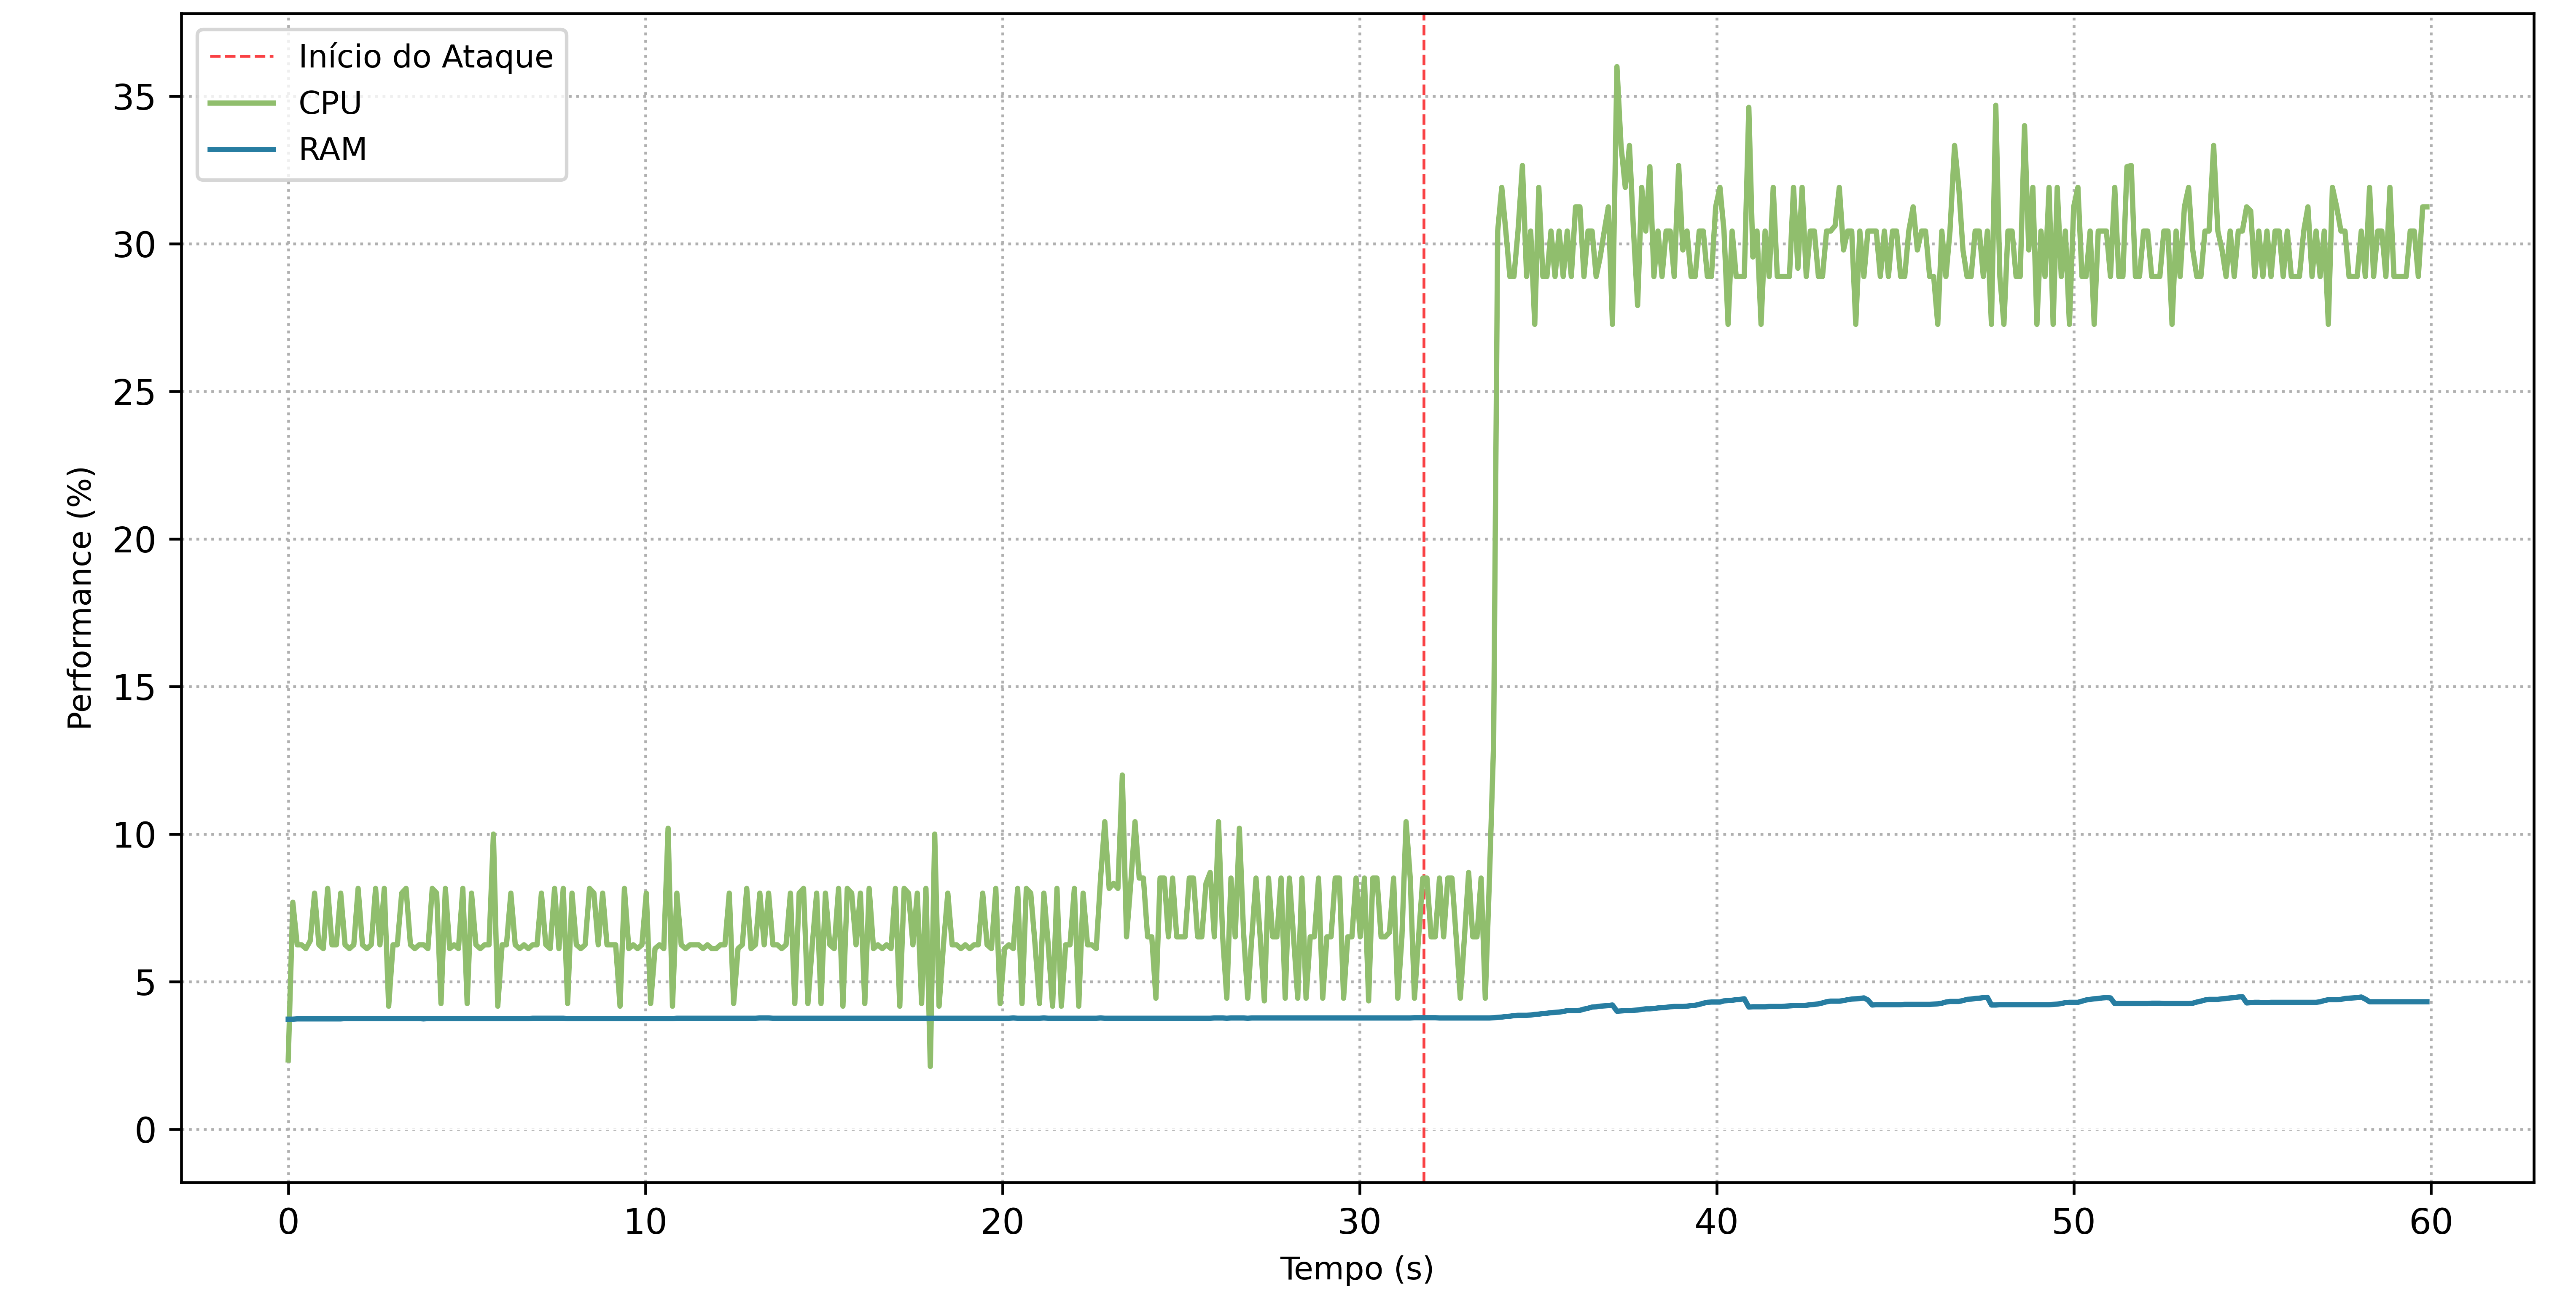
\includegraphics[width=1\textwidth, height=120pt]{USPSC-img/output/cropped/0-dos_function_call_null_deref-perf.png}
        \caption{Desempenho}
    \end{subfigure}%
    \\
    \begin{subfigure}[t]{0.5\textwidth}
        \centering
        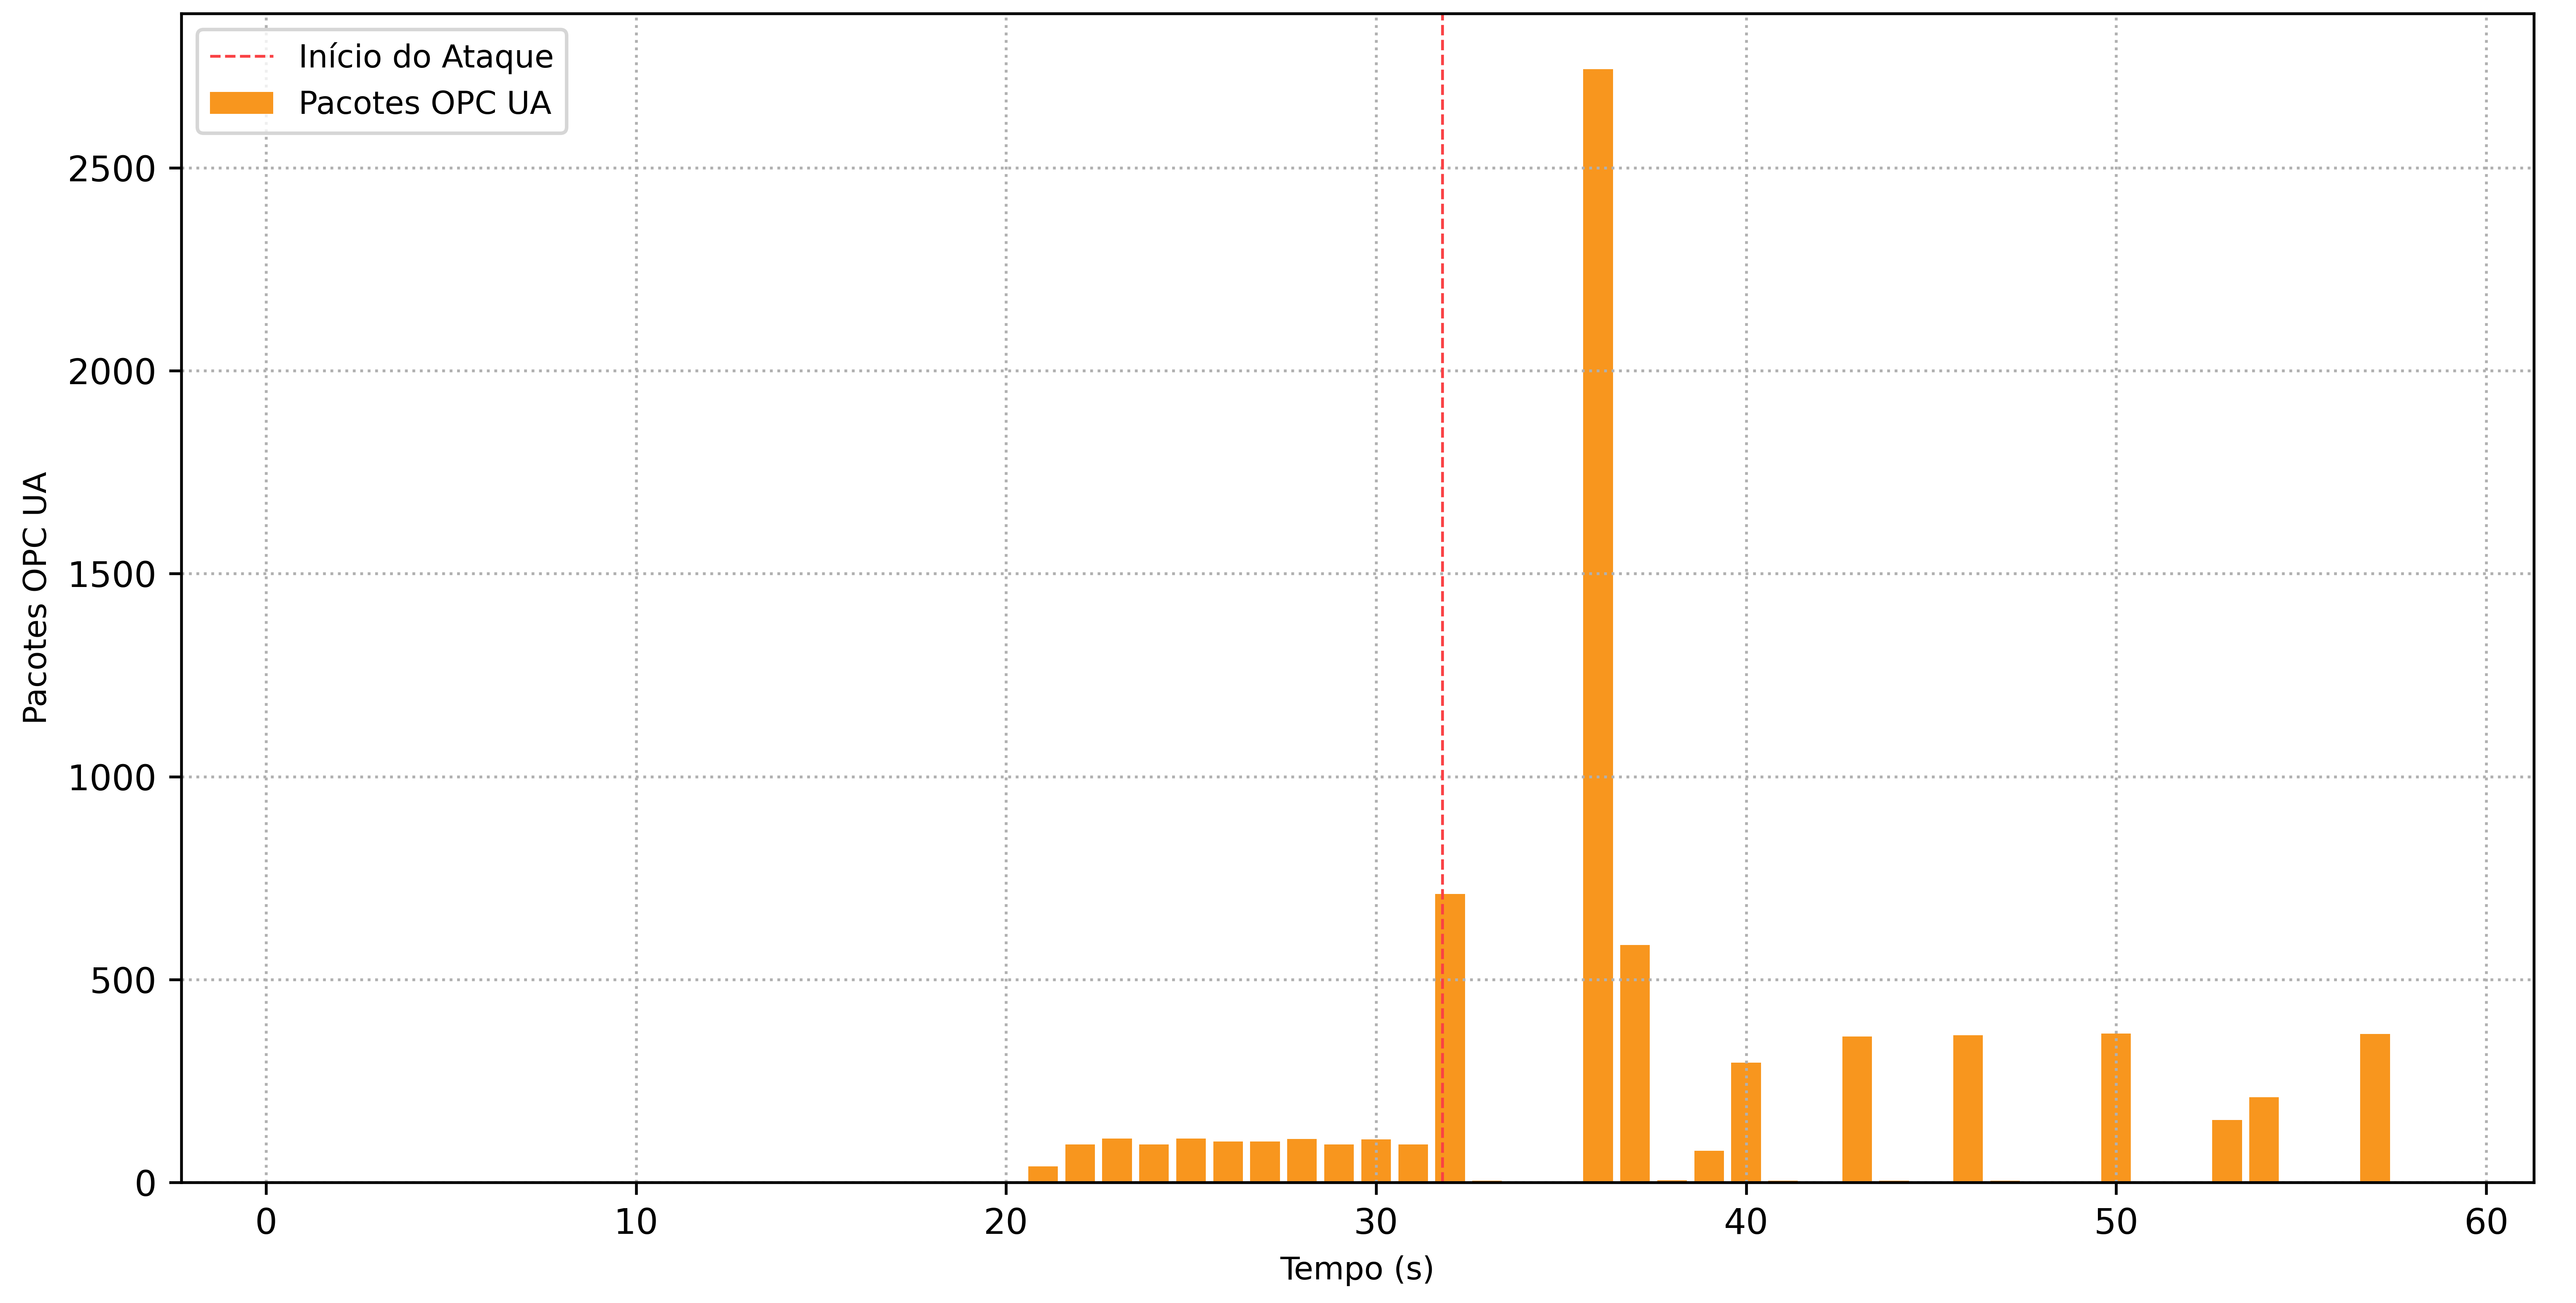
\includegraphics[width=1\textwidth, height=120pt]{USPSC-img/output/cropped/0-dos_function_call_null_deref-pack.png}
        \caption{Pacotes OPC UA}
    \end{subfigure}%
    ~
    \begin{subfigure}[t]{0.5\textwidth}
        \centering
        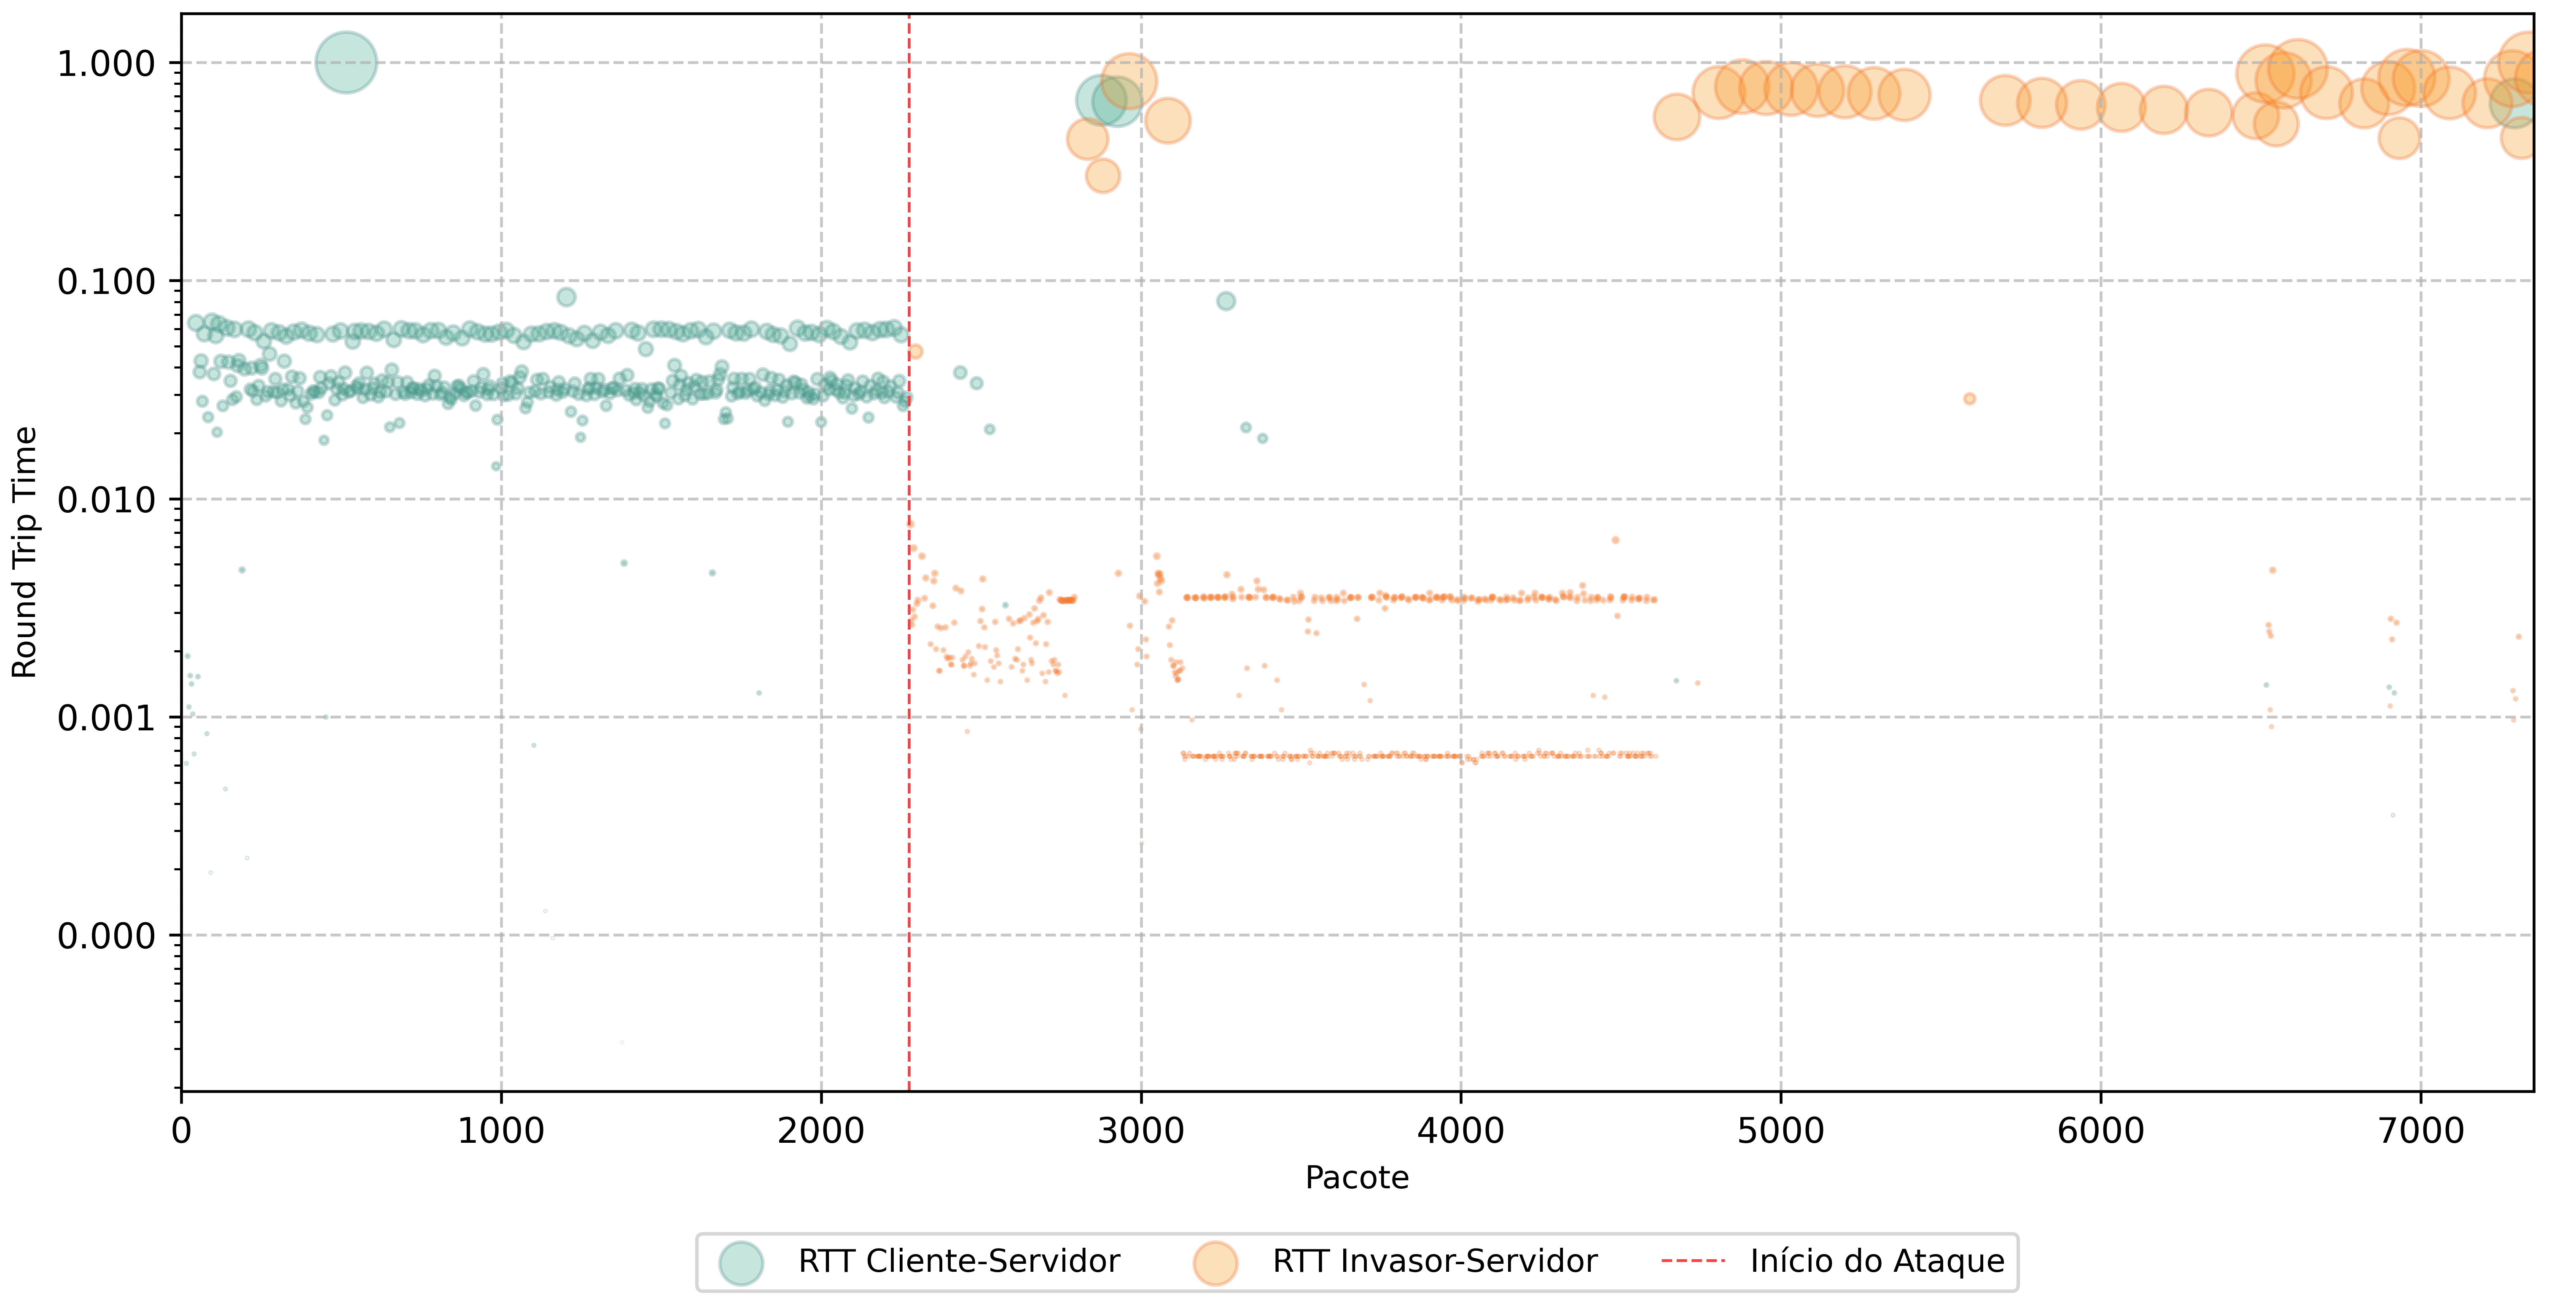
\includegraphics[width=1\textwidth, height=120pt]{USPSC-img/output/cropped/0-dos_function_call_null_deref-rttp.png}
        \caption{RTT por pacote}
    \end{subfigure}%
    % ~
    % \begin{subfigure}[t]{0.5\textwidth}
    %     \centering
    %     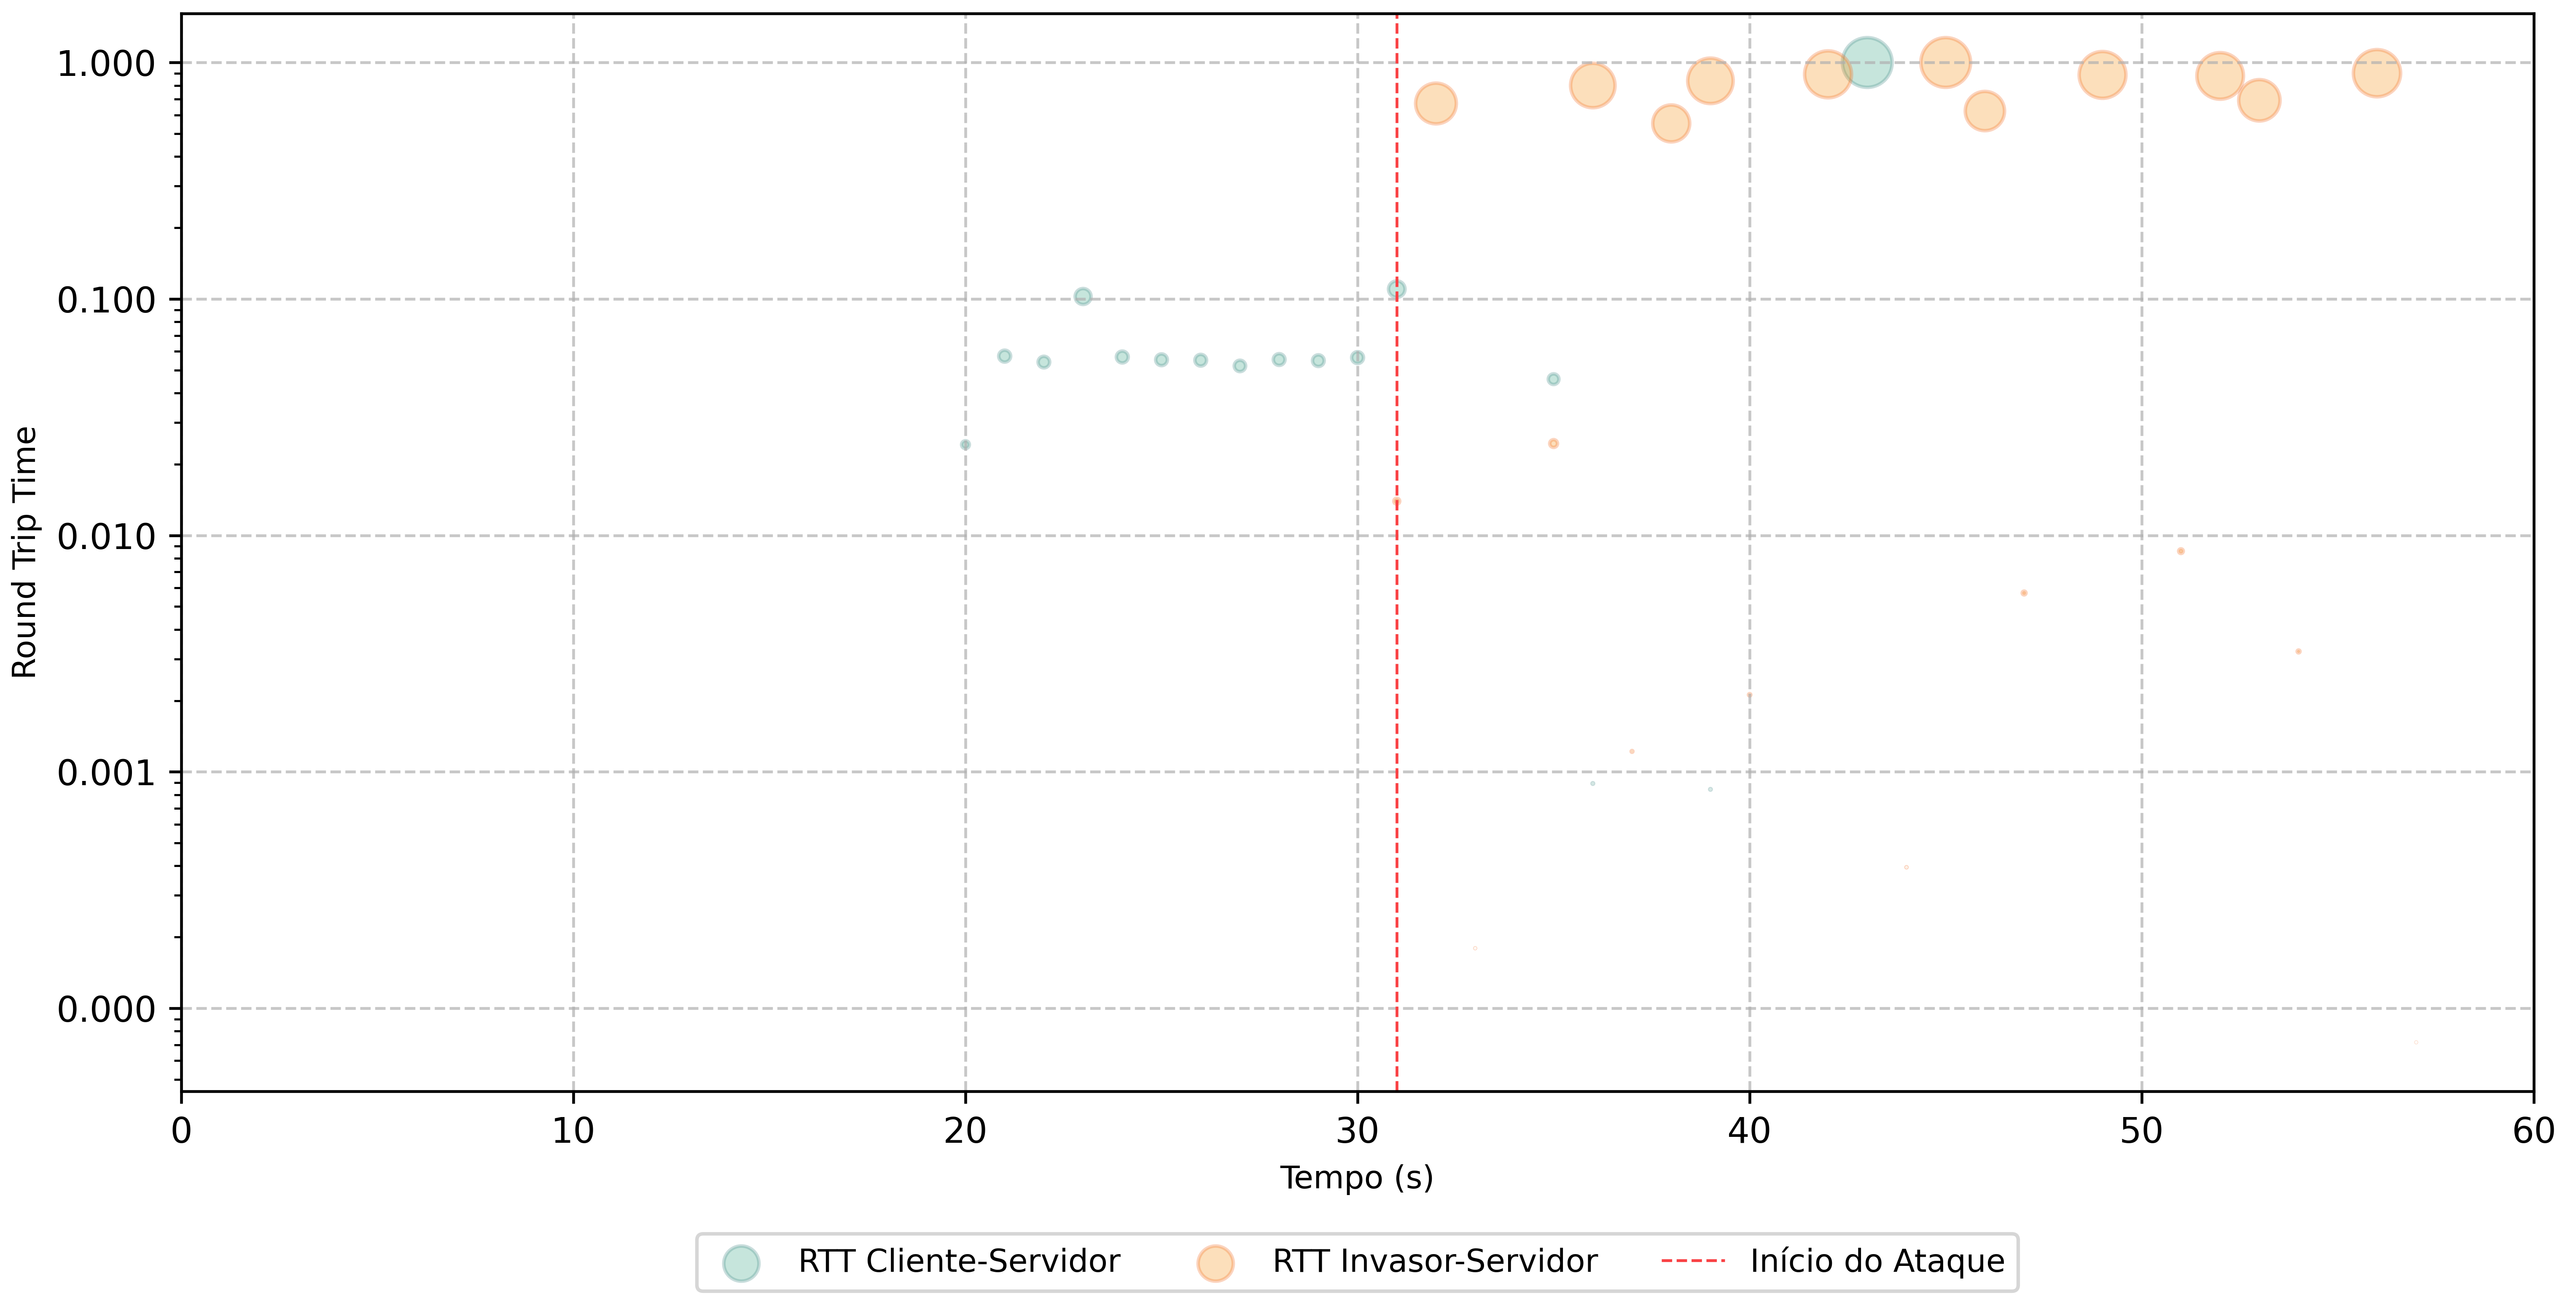
\includegraphics[width=1\textwidth, height=120pt]{USPSC-img/output/cropped/0-dos_function_call_null_deref-rtts.png}
    %     \caption{RTT por segundos}
    % \end{subfigure}%
    \label{fig:0-dos_function_call_null_deref}
    \caption{Gráficos do ataque de DoS pela chamada da função \textit{Dereference} nula - nível de segurança: `None'.}
\end{figure}

\begin{figure}[htbp!]
    \centering
    \begin{subfigure}[t]{0.5\textwidth}
        \centering
        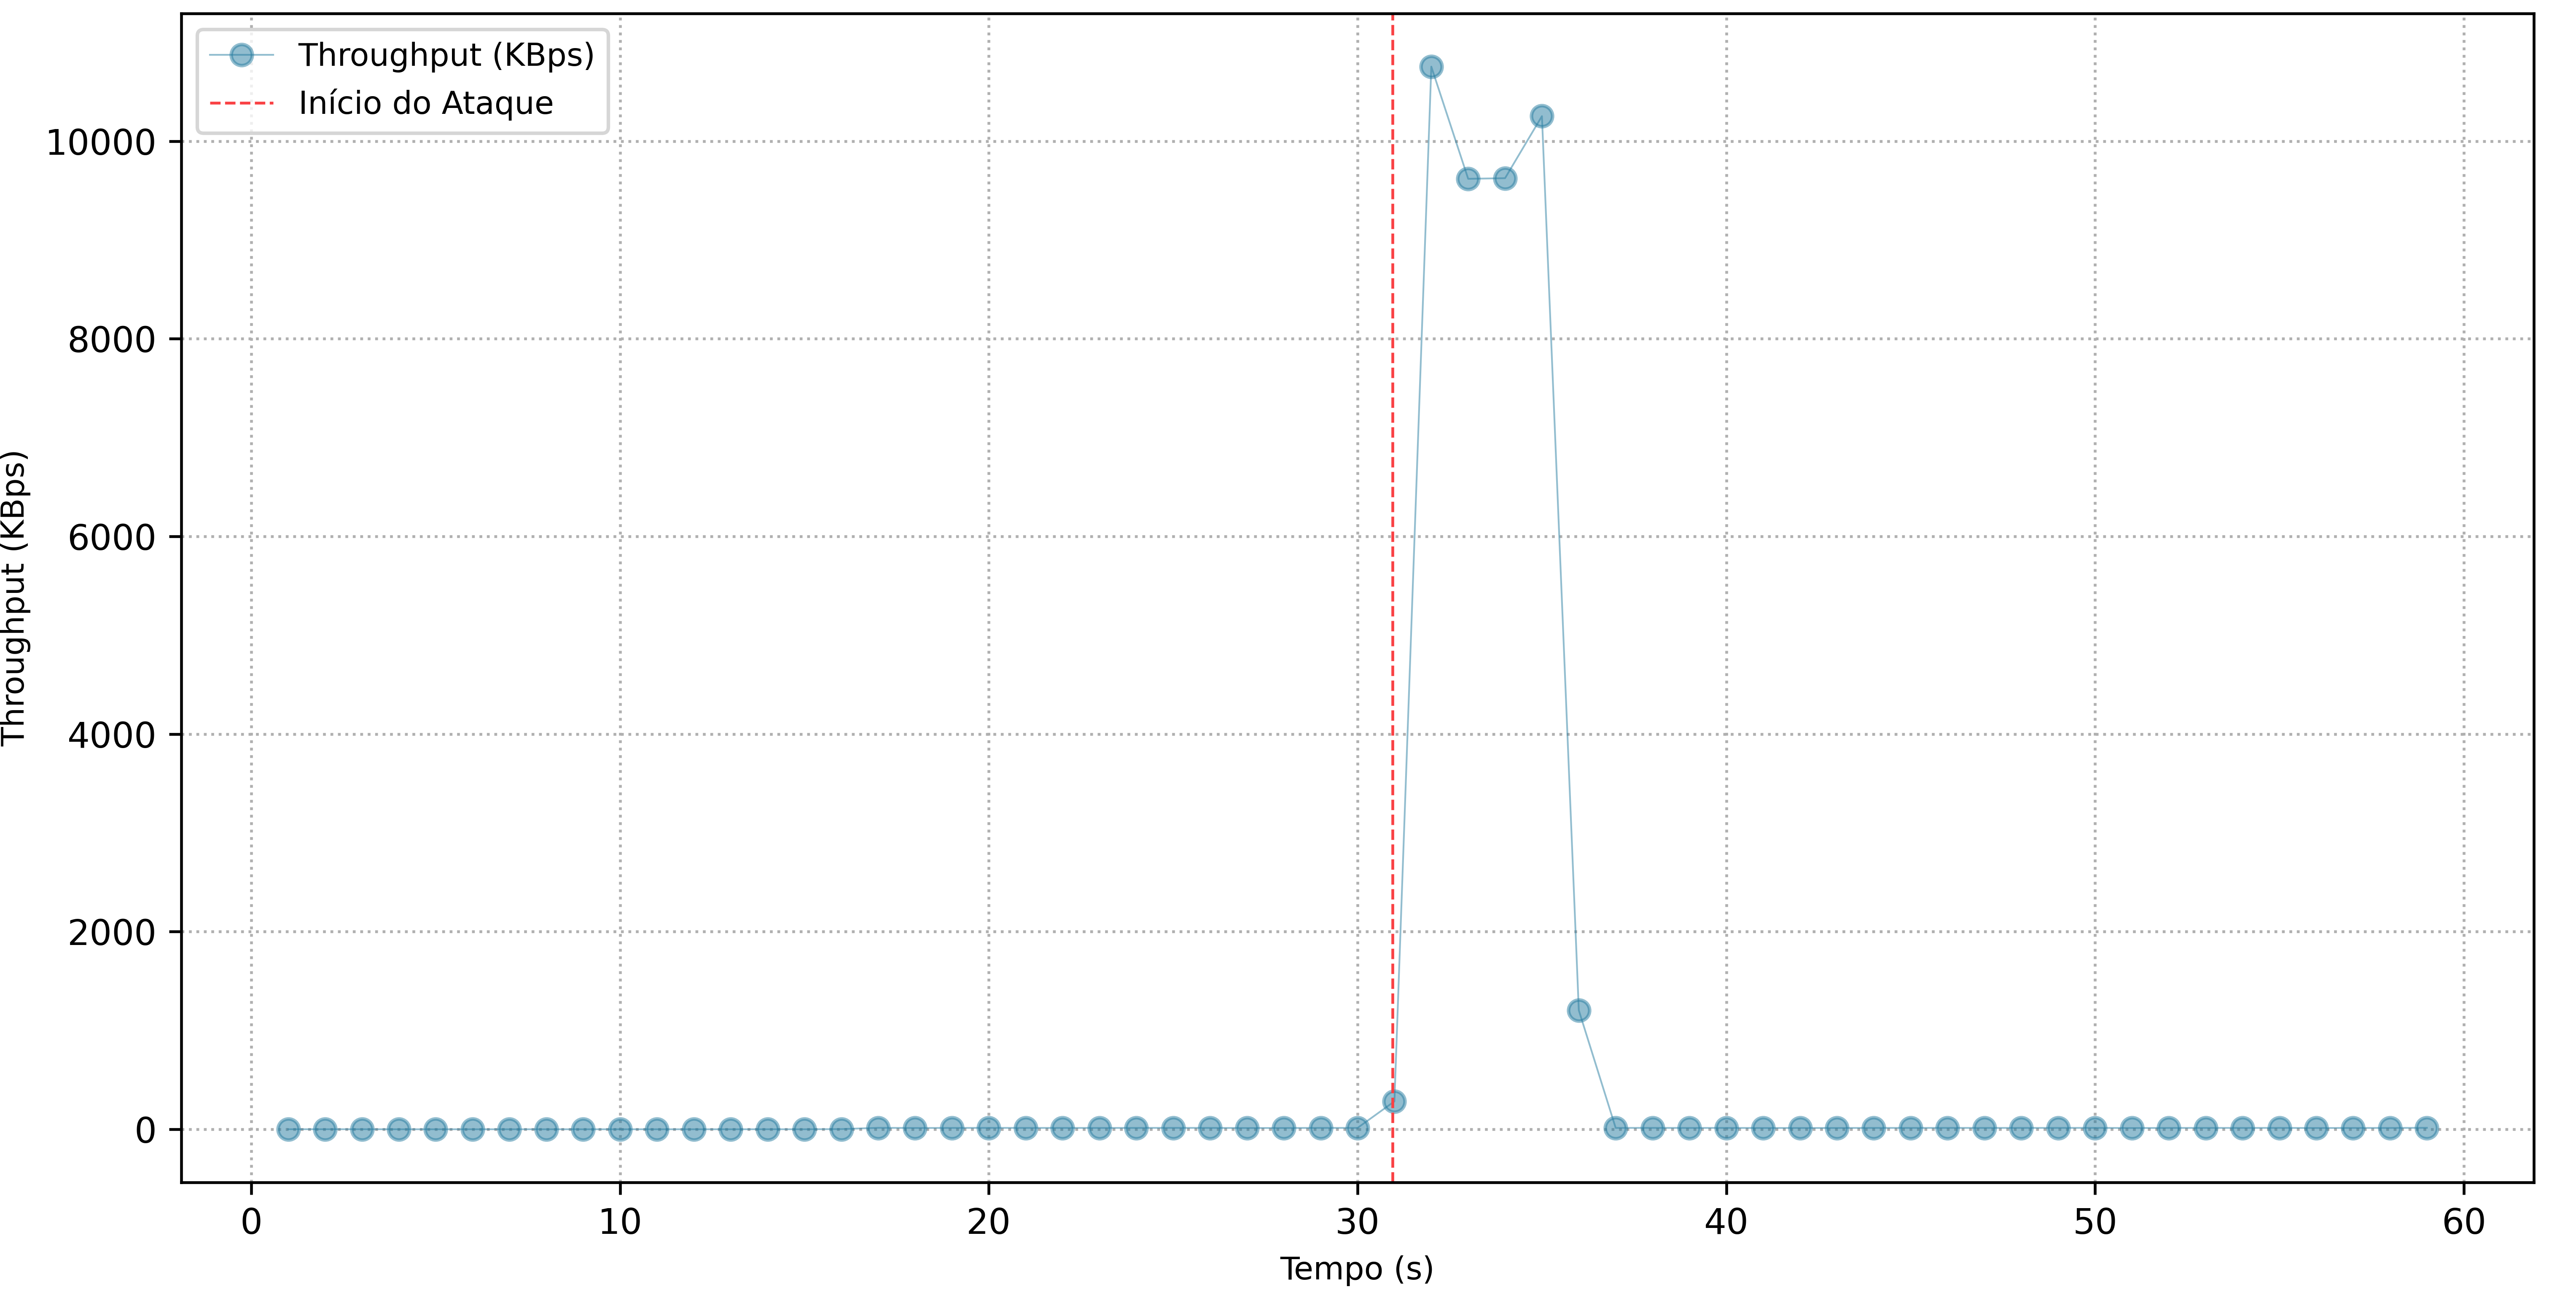
\includegraphics[width=1\textwidth, height=120pt]{USPSC-img/output/cropped/1-dos_function_call_null_deref-tput.png}
        \caption{\textit{Throughput}}
    \end{subfigure}%
    ~ 
    \begin{subfigure}[t]{0.5\textwidth}
        \centering
        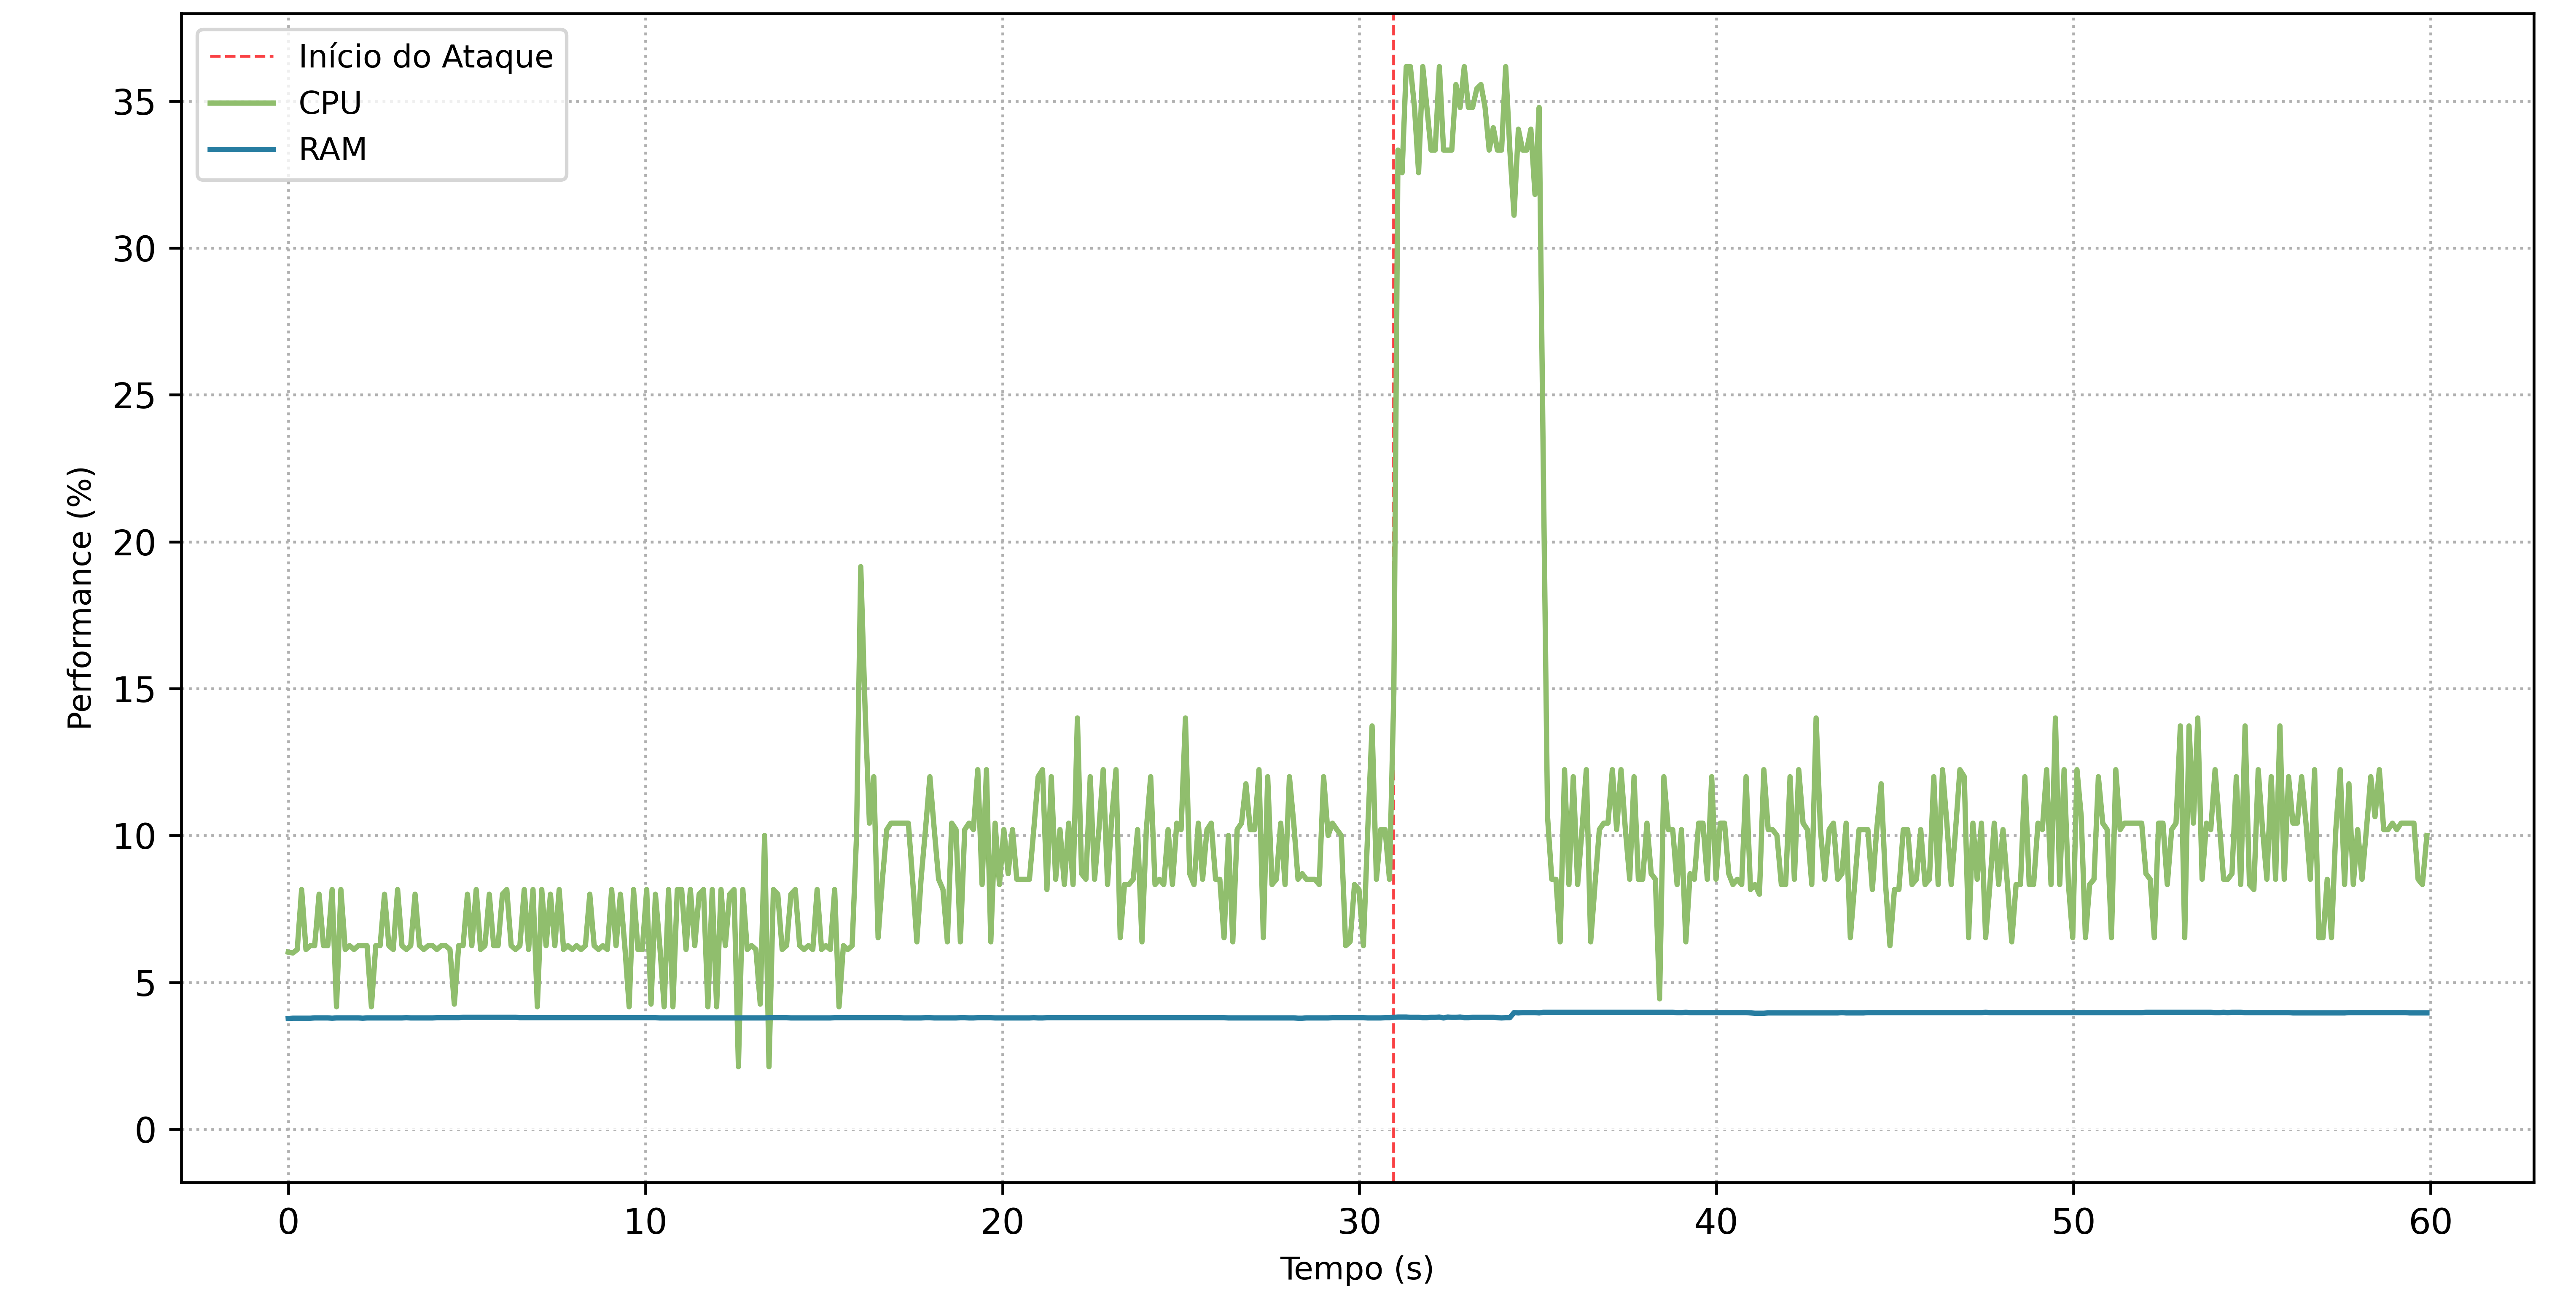
\includegraphics[width=1\textwidth, height=120pt]{USPSC-img/output/cropped/1-dos_function_call_null_deref-perf.png}
        \caption{Desempenho}
    \end{subfigure}%
    \\
    \begin{subfigure}[t]{0.5\textwidth}
        \centering
        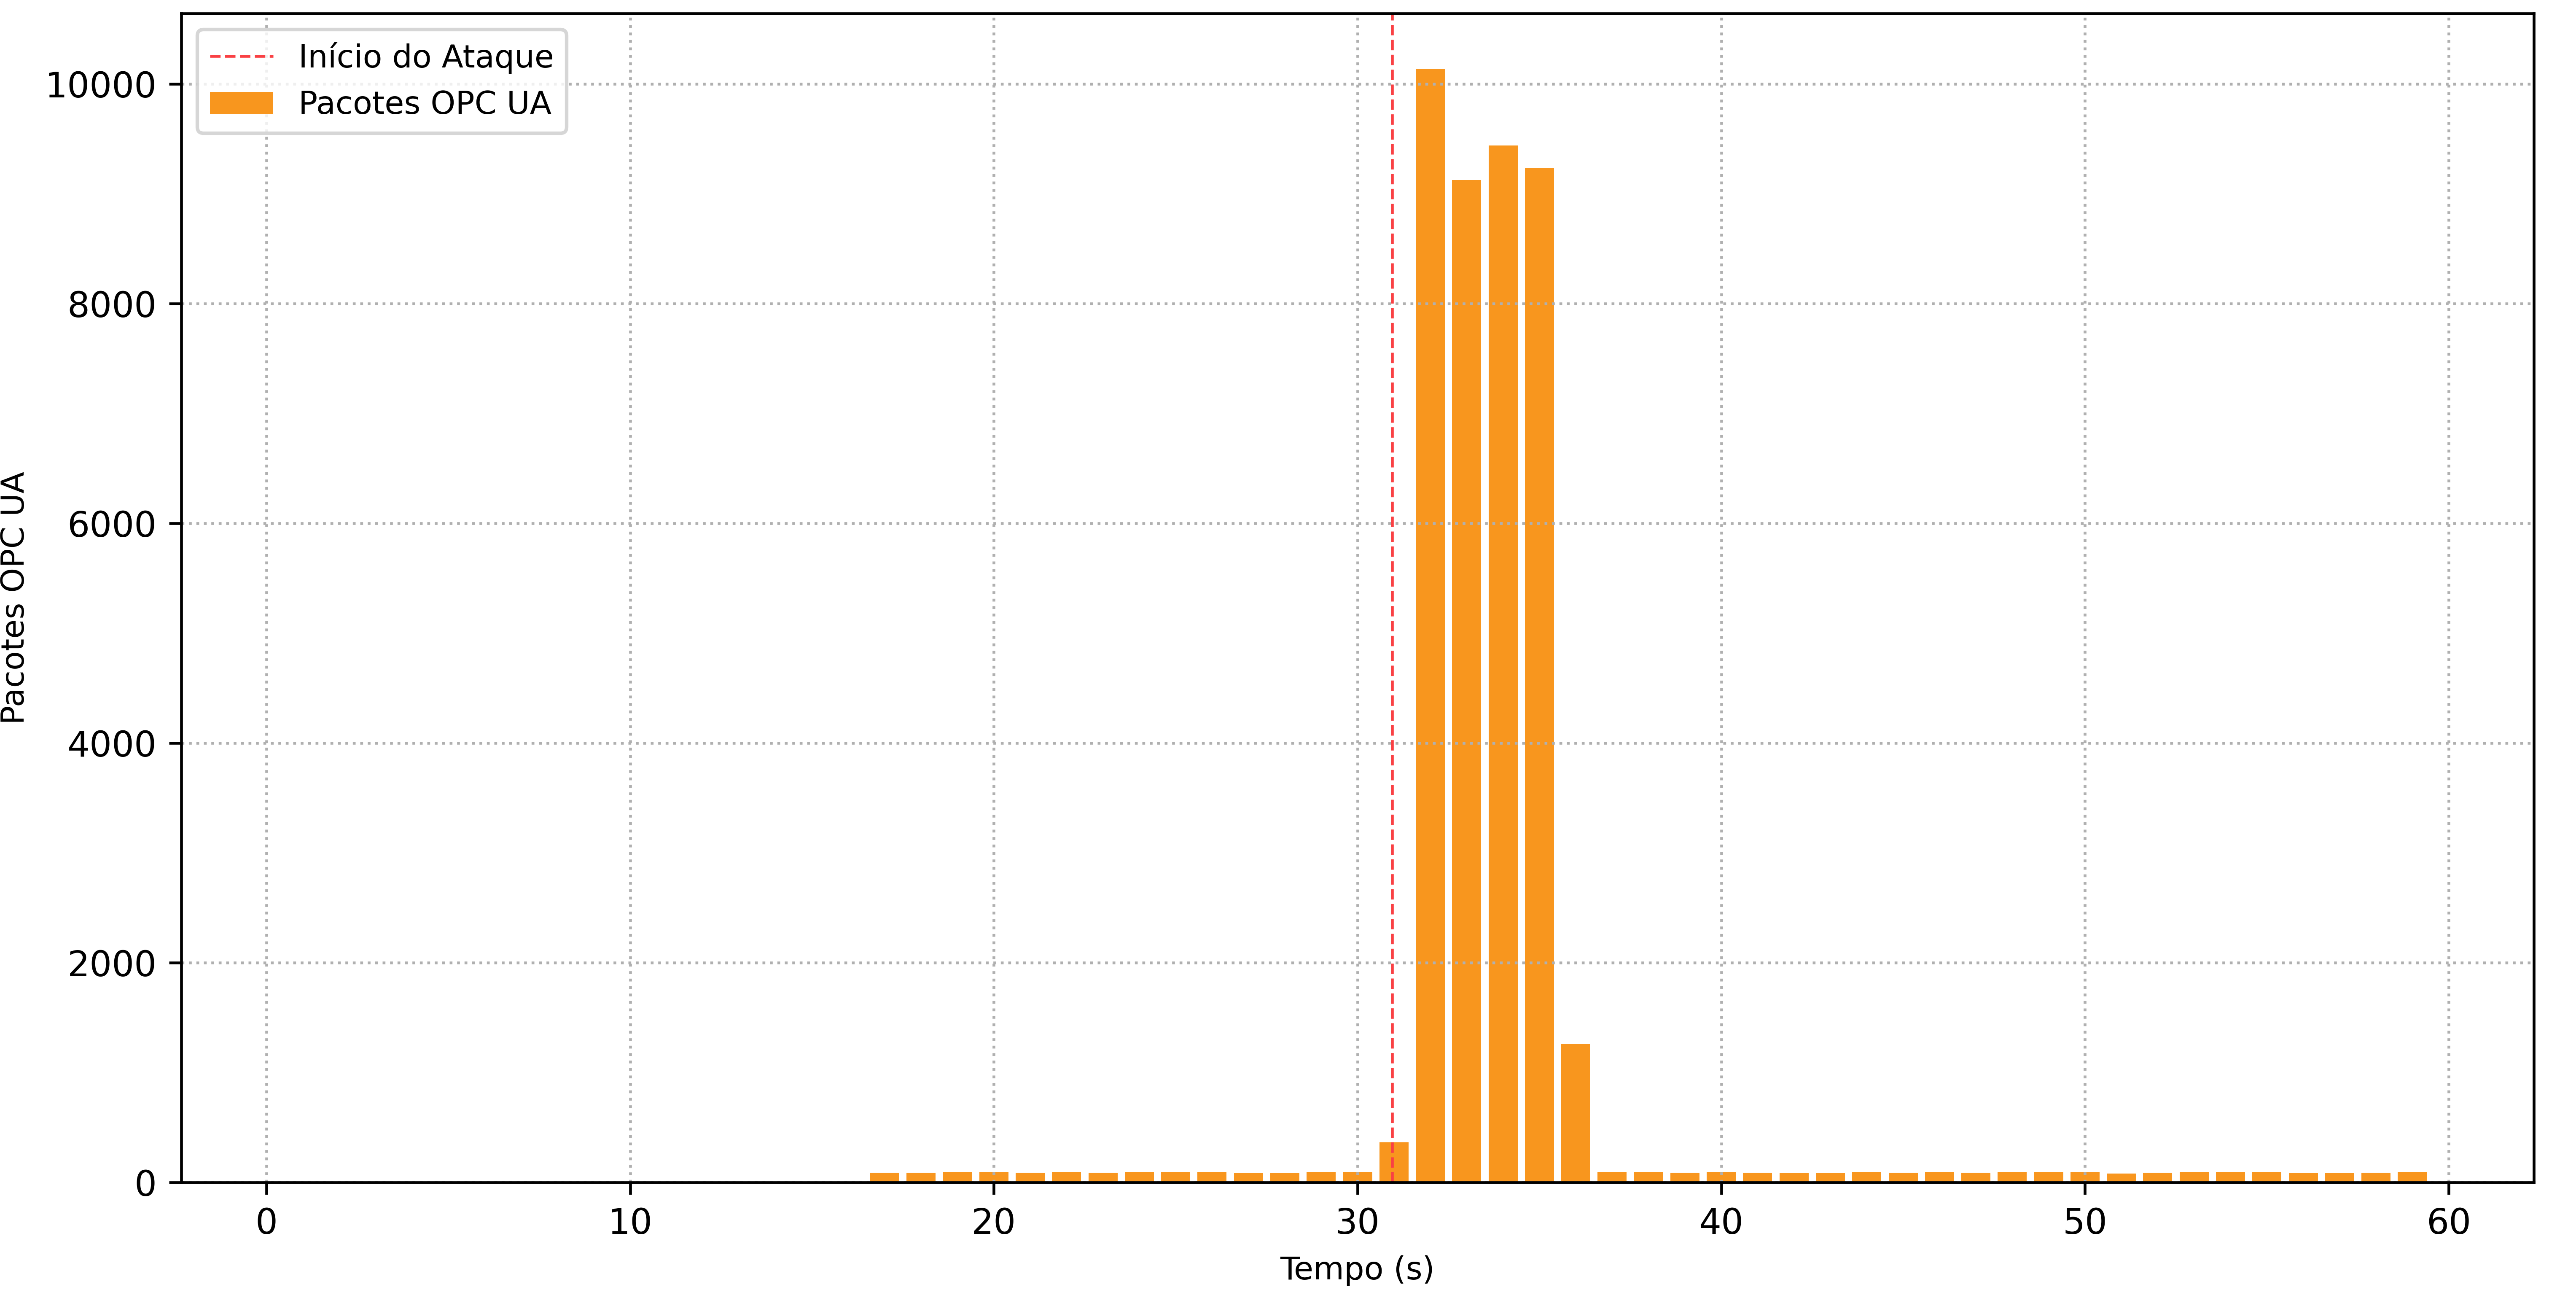
\includegraphics[width=1\textwidth, height=120pt]{USPSC-img/output/cropped/1-dos_function_call_null_deref-pack.png}
        \caption{Pacotes OPC UA}
    \end{subfigure}%
    ~
    \begin{subfigure}[t]{0.5\textwidth}
        \centering
        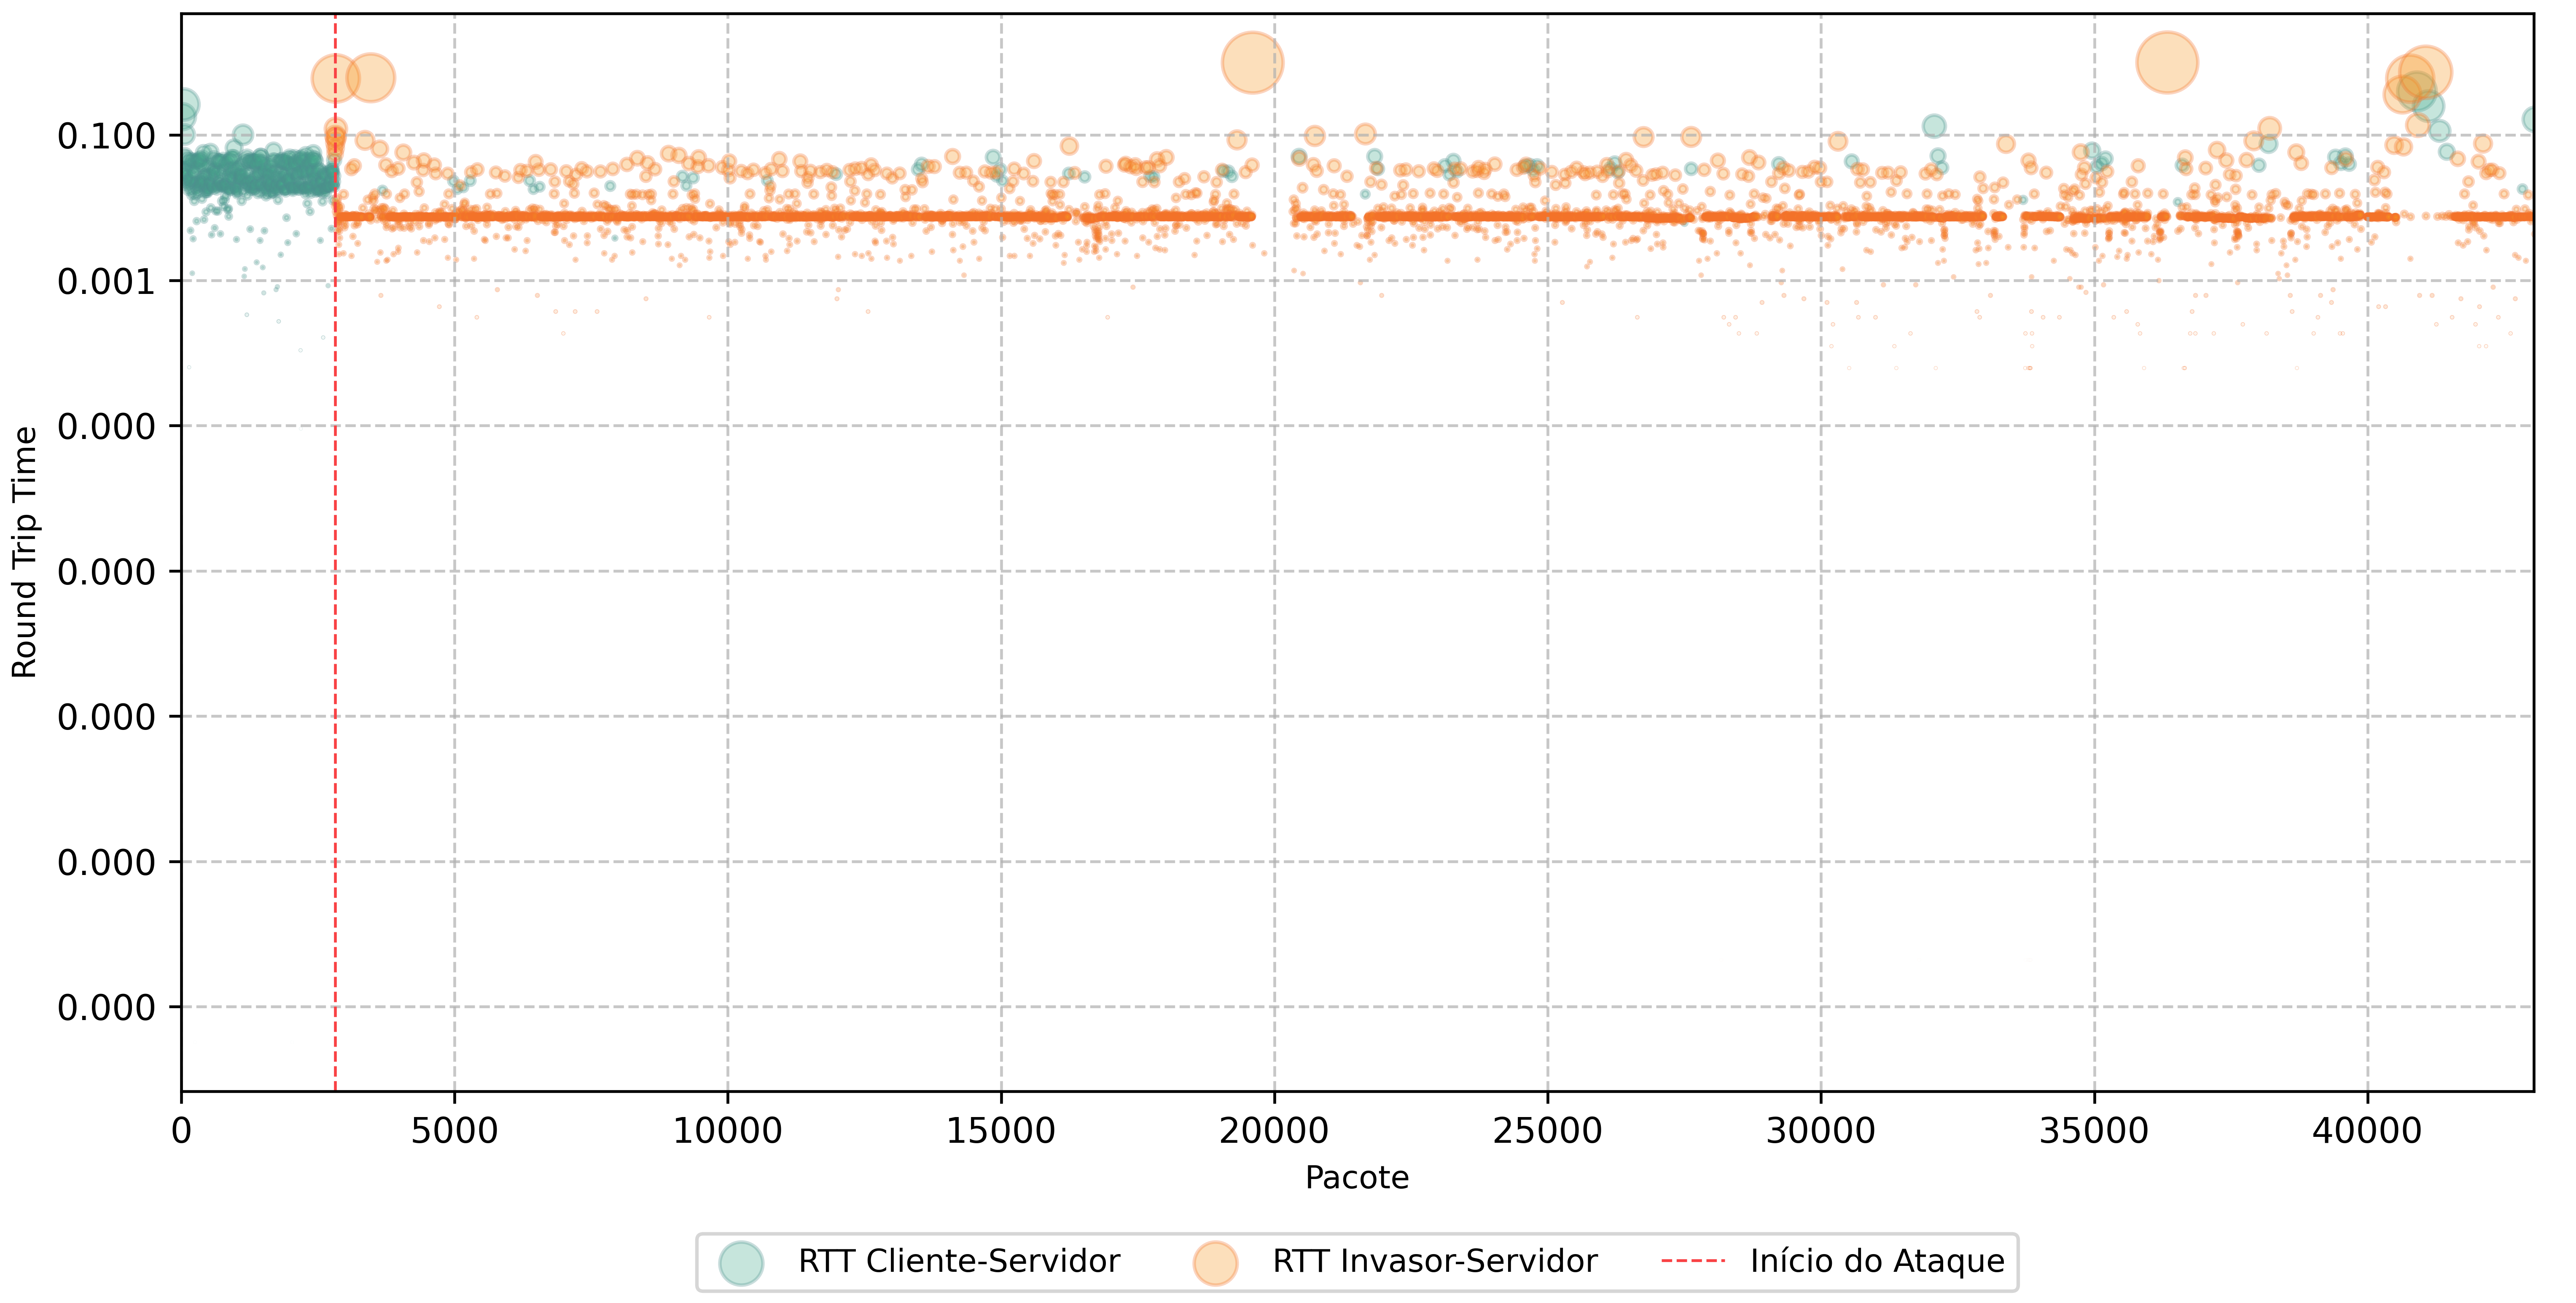
\includegraphics[width=1\textwidth, height=120pt]{USPSC-img/output/cropped/1-dos_function_call_null_deref-rttp.png}
        \caption{RTT por pacote}
    \end{subfigure}%
    % ~
    % \begin{subfigure}[t]{0.5\textwidth}
    %     \centering
    %     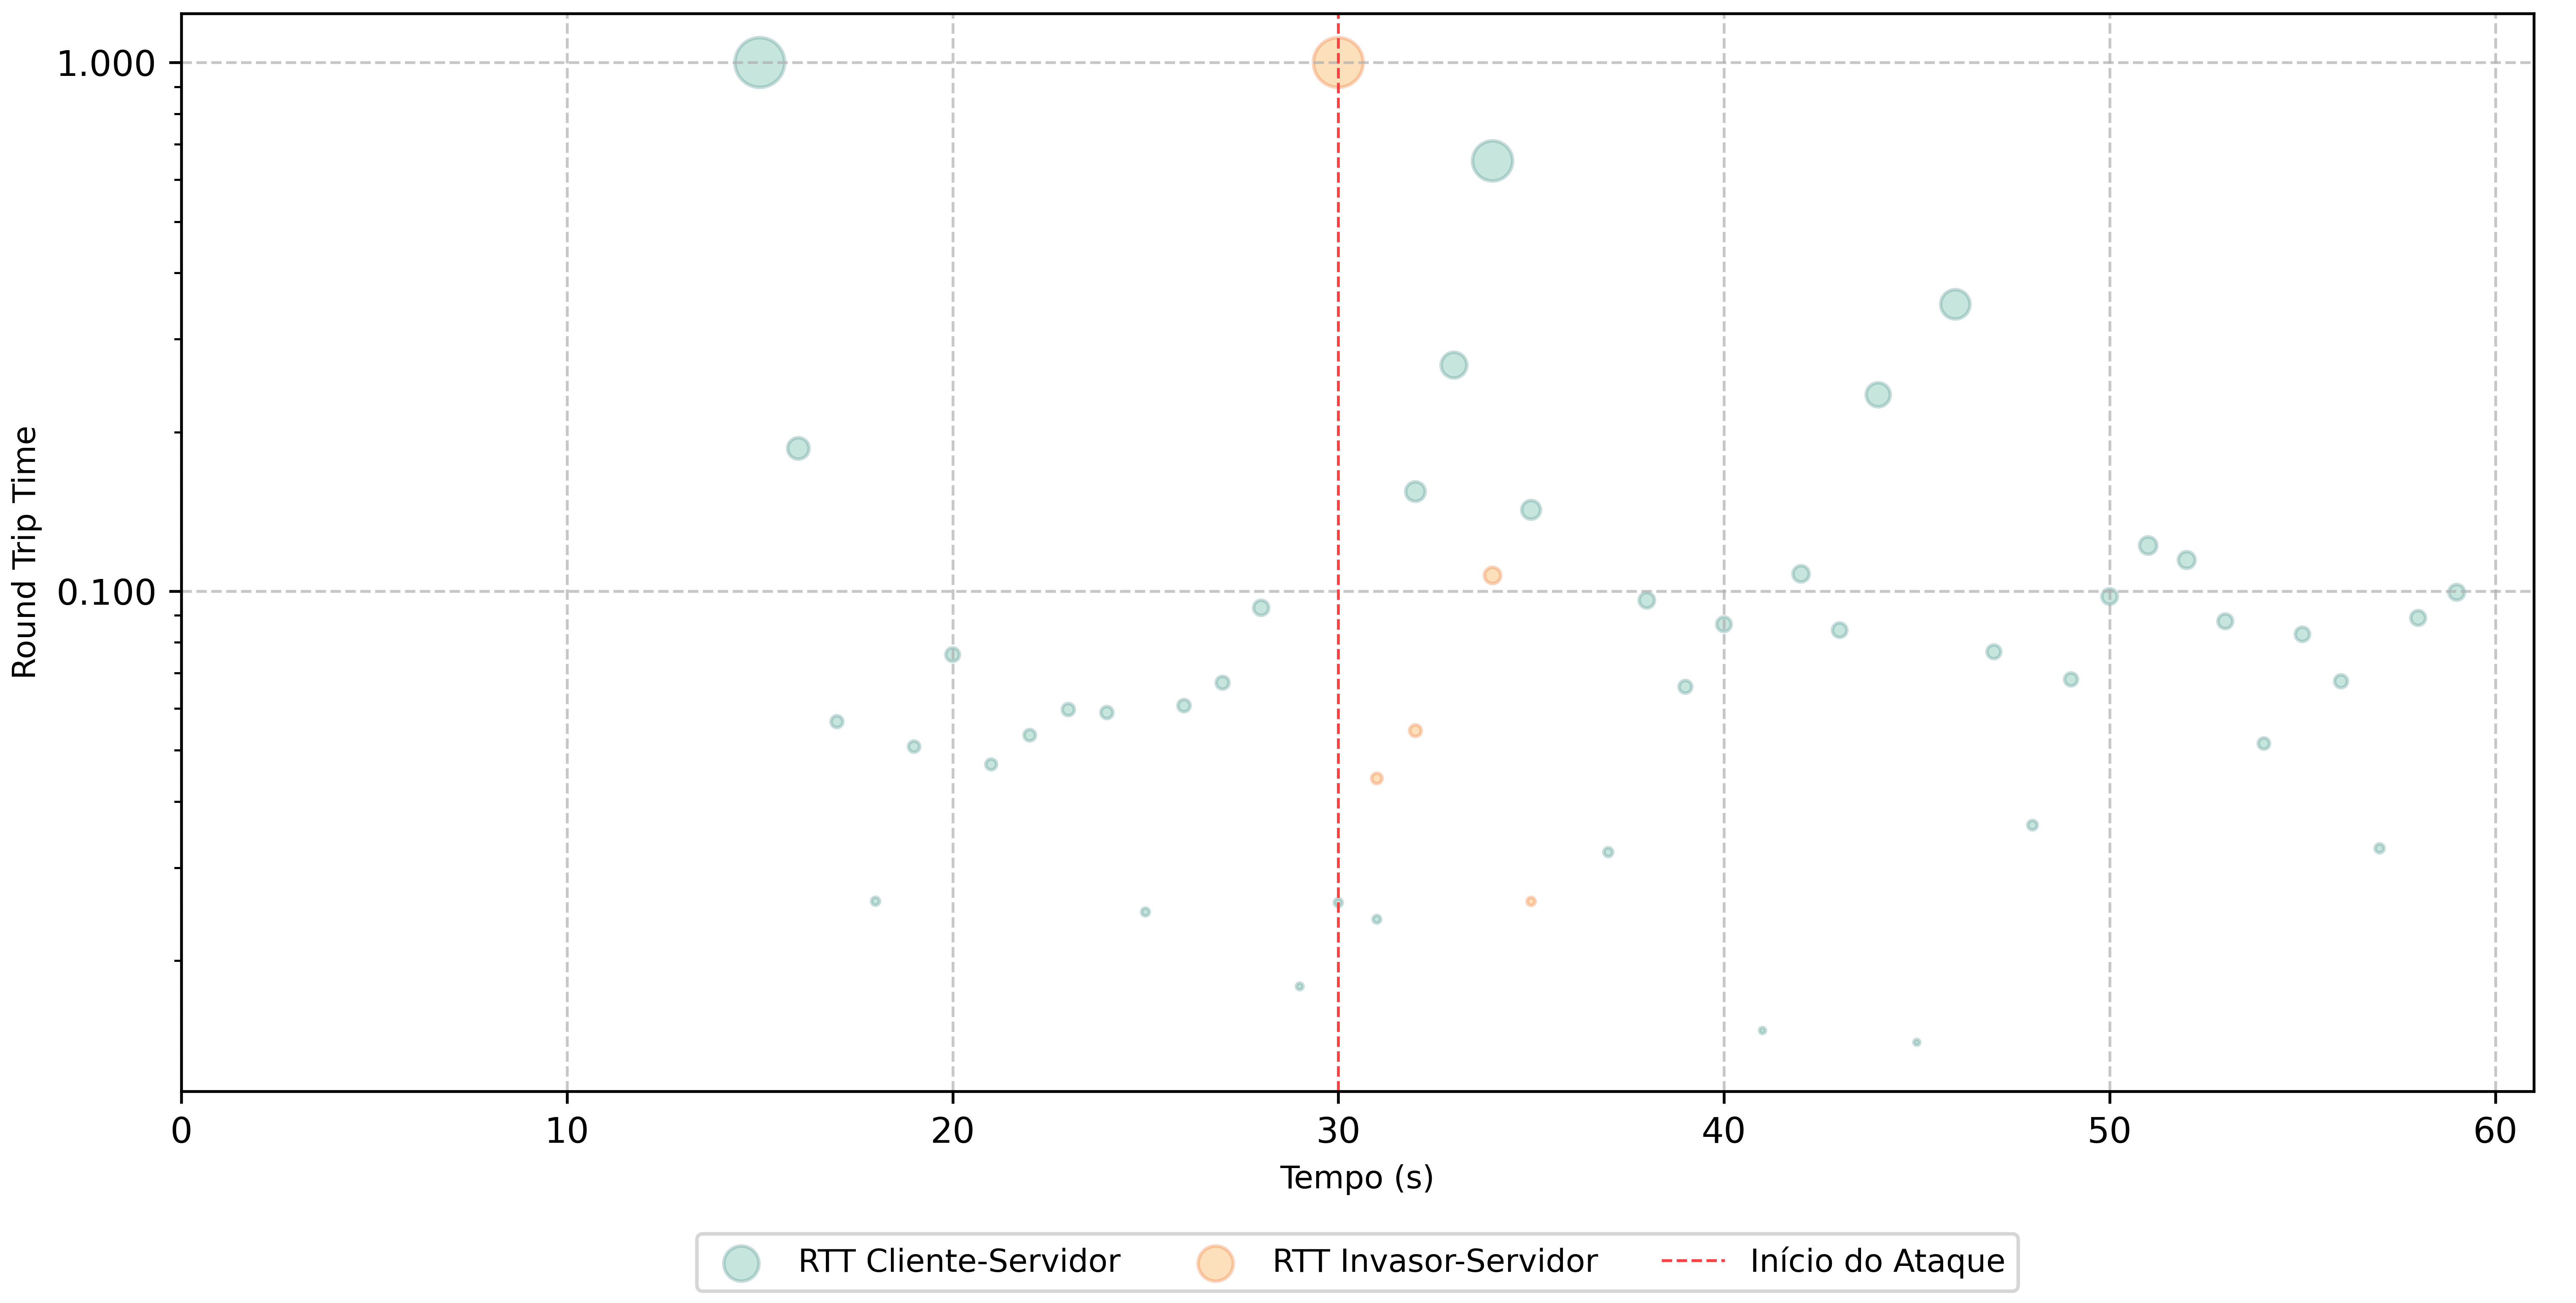
\includegraphics[width=1\textwidth, height=120pt]{USPSC-img/output/cropped/1-dos_function_call_null_deref-rtts.png}
    %     \caption{RTT por segundos}
    % \end{subfigure}%
    \label{fig:1-dos_function_call_null_deref}
    \caption{Gráficos do ataque de DoS pela chamada da função \textit{Dereference} nula - nível de segurança: `Sign'.}
\end{figure}

\begin{figure}[htbp!]
    \centering
    \begin{subfigure}[t]{0.5\textwidth}
        \centering
        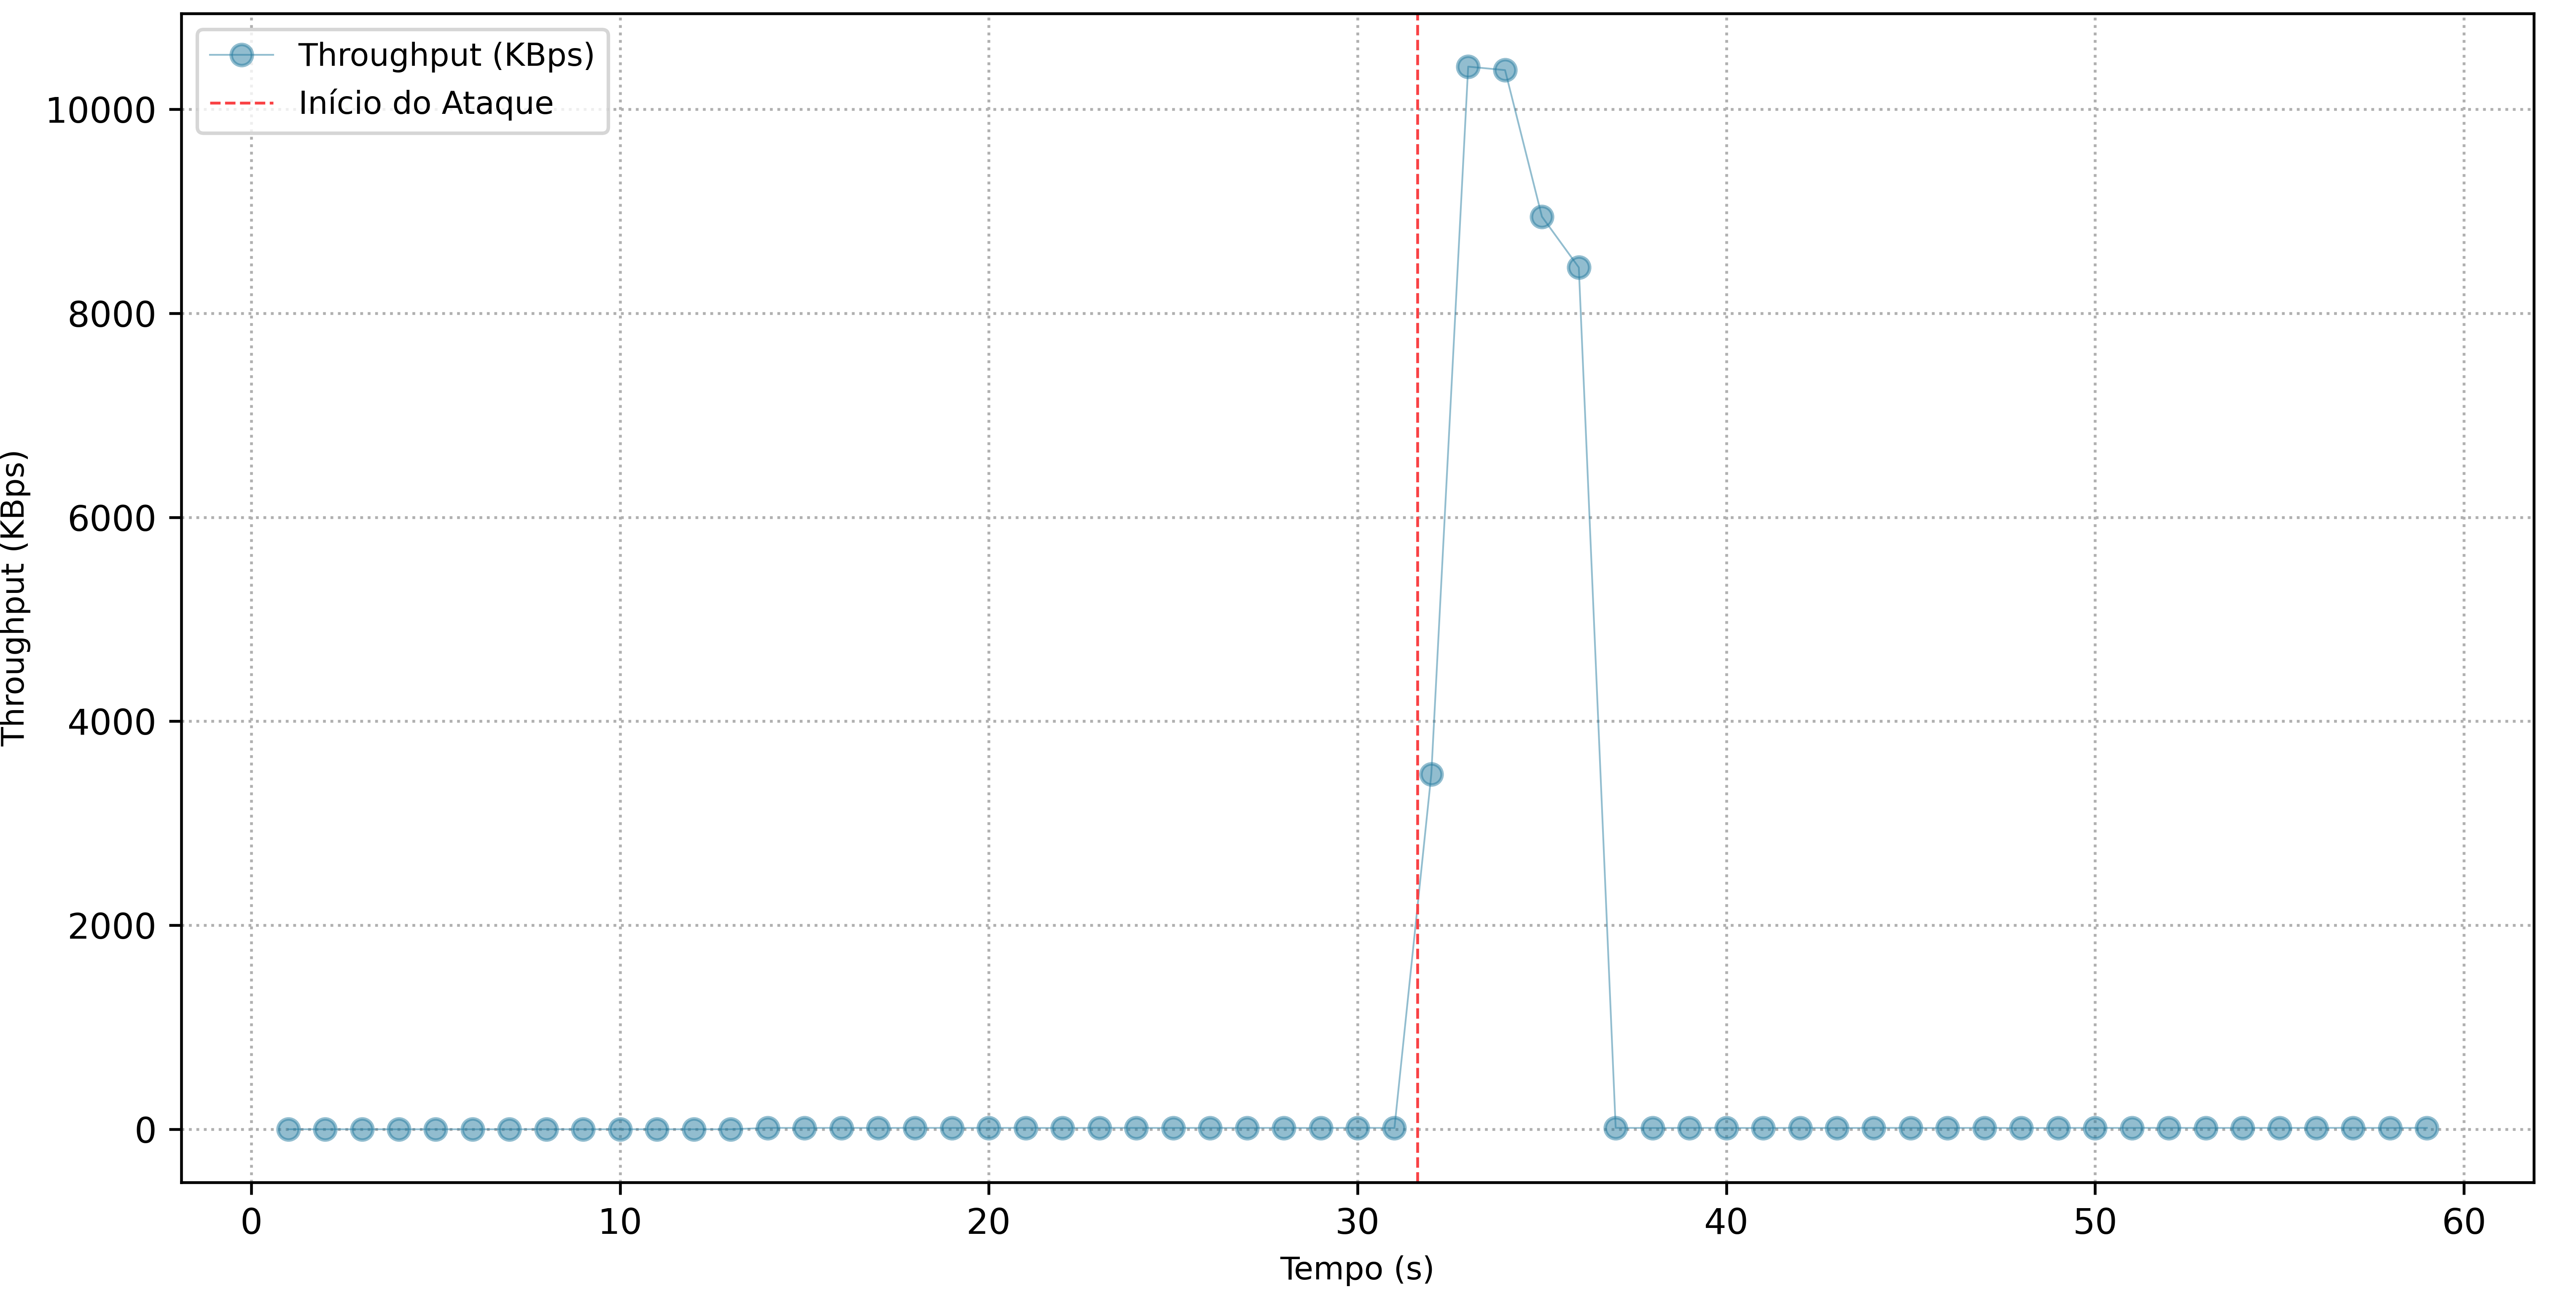
\includegraphics[width=1\textwidth, height=120pt]{USPSC-img/output/cropped/2-dos_function_call_null_deref-tput.png}
        \caption{\textit{Throughput}}
    \end{subfigure}%
    ~ 
    \begin{subfigure}[t]{0.5\textwidth}
        \centering
        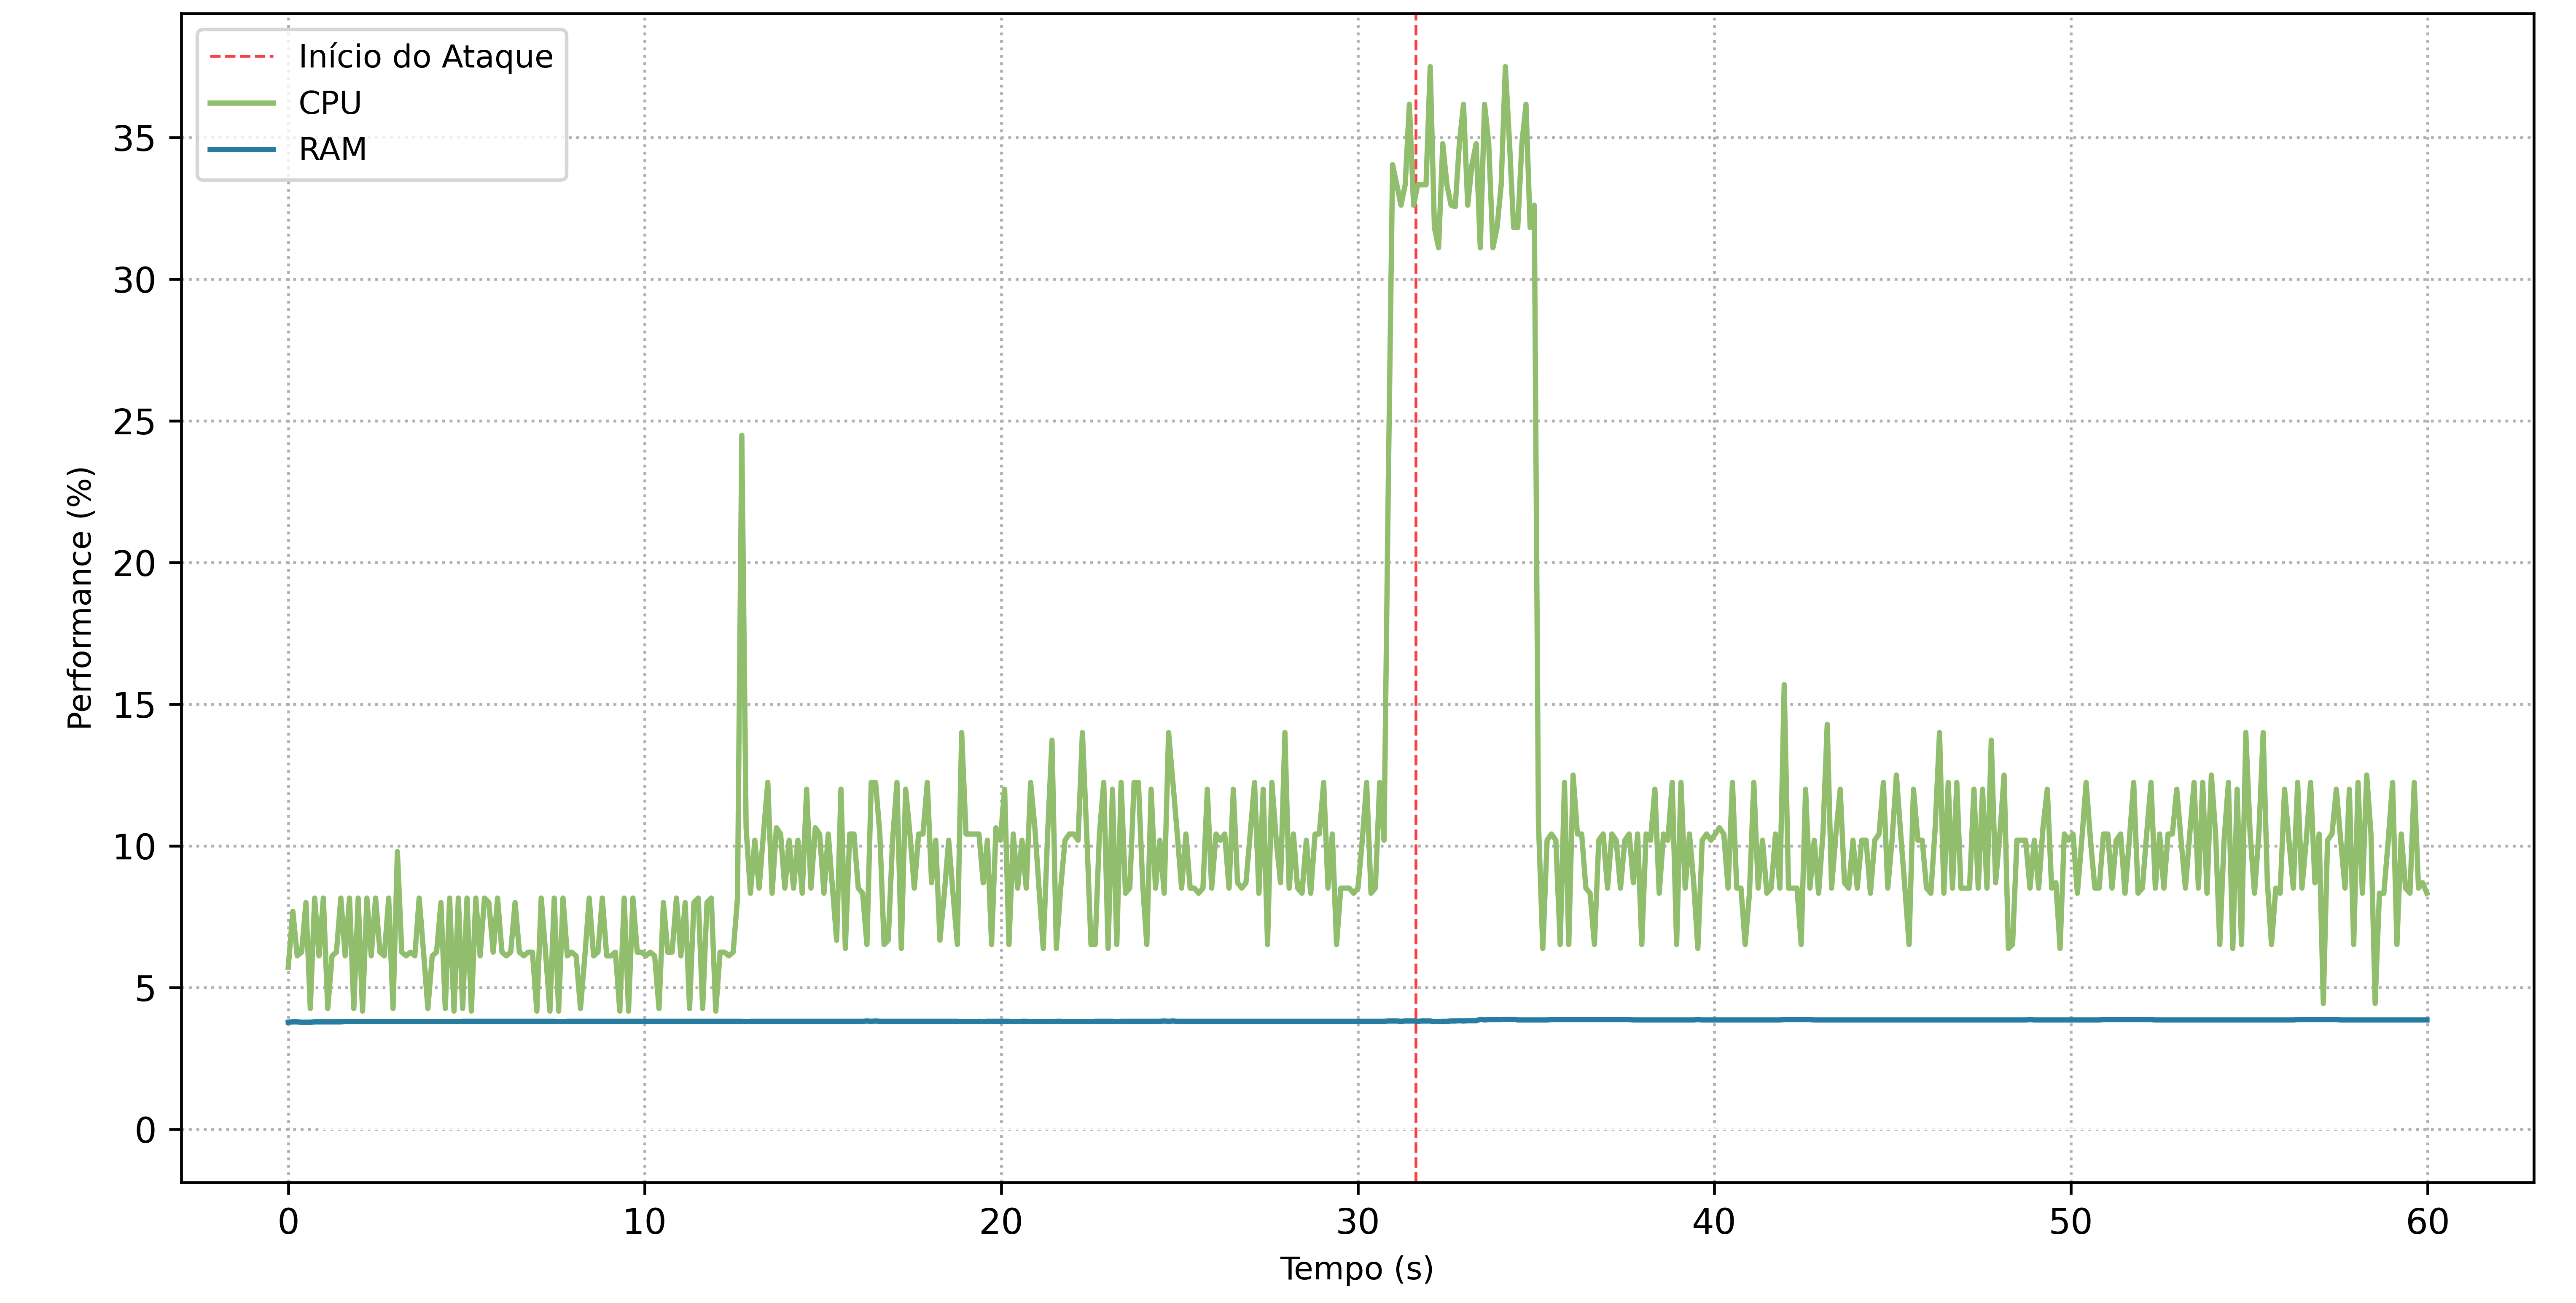
\includegraphics[width=1\textwidth, height=120pt]{USPSC-img/output/cropped/2-dos_function_call_null_deref-perf.png}
        \caption{Desempenho}
    \end{subfigure}%
    \\
    \begin{subfigure}[t]{0.5\textwidth}
        \centering
        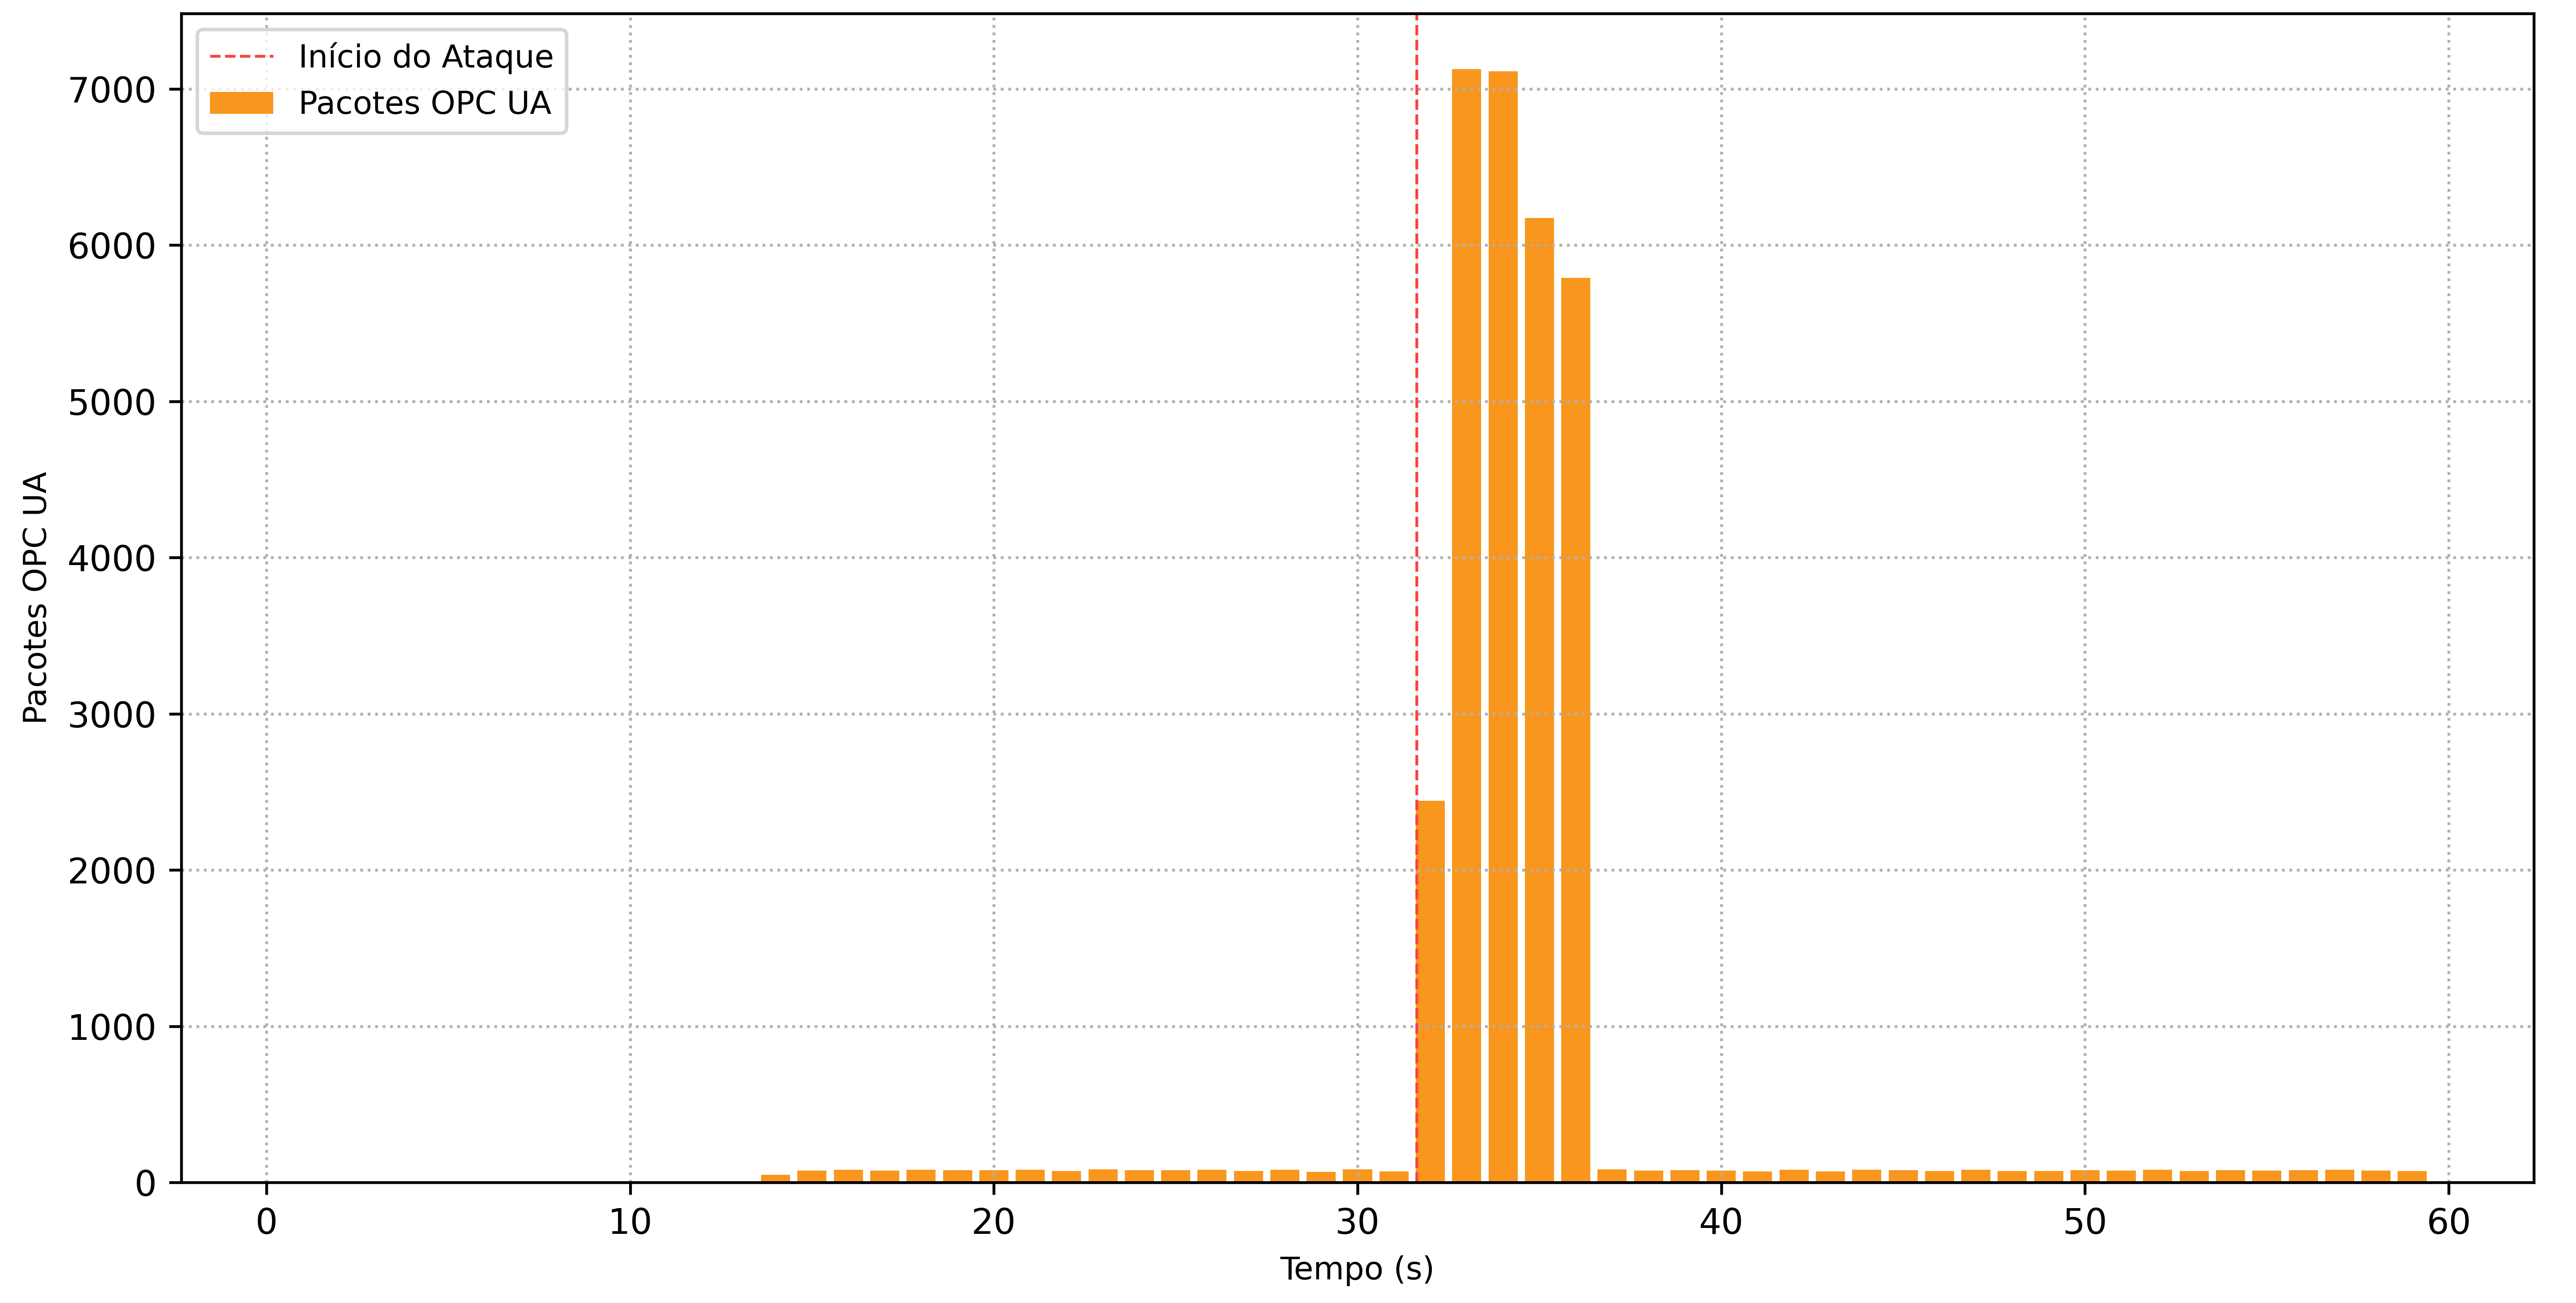
\includegraphics[width=1\textwidth, height=120pt]{USPSC-img/output/cropped/2-dos_function_call_null_deref-pack.png}
        \caption{Pacotes OPC UA}
    \end{subfigure}%
    ~
    \begin{subfigure}[t]{0.5\textwidth}
        \centering
        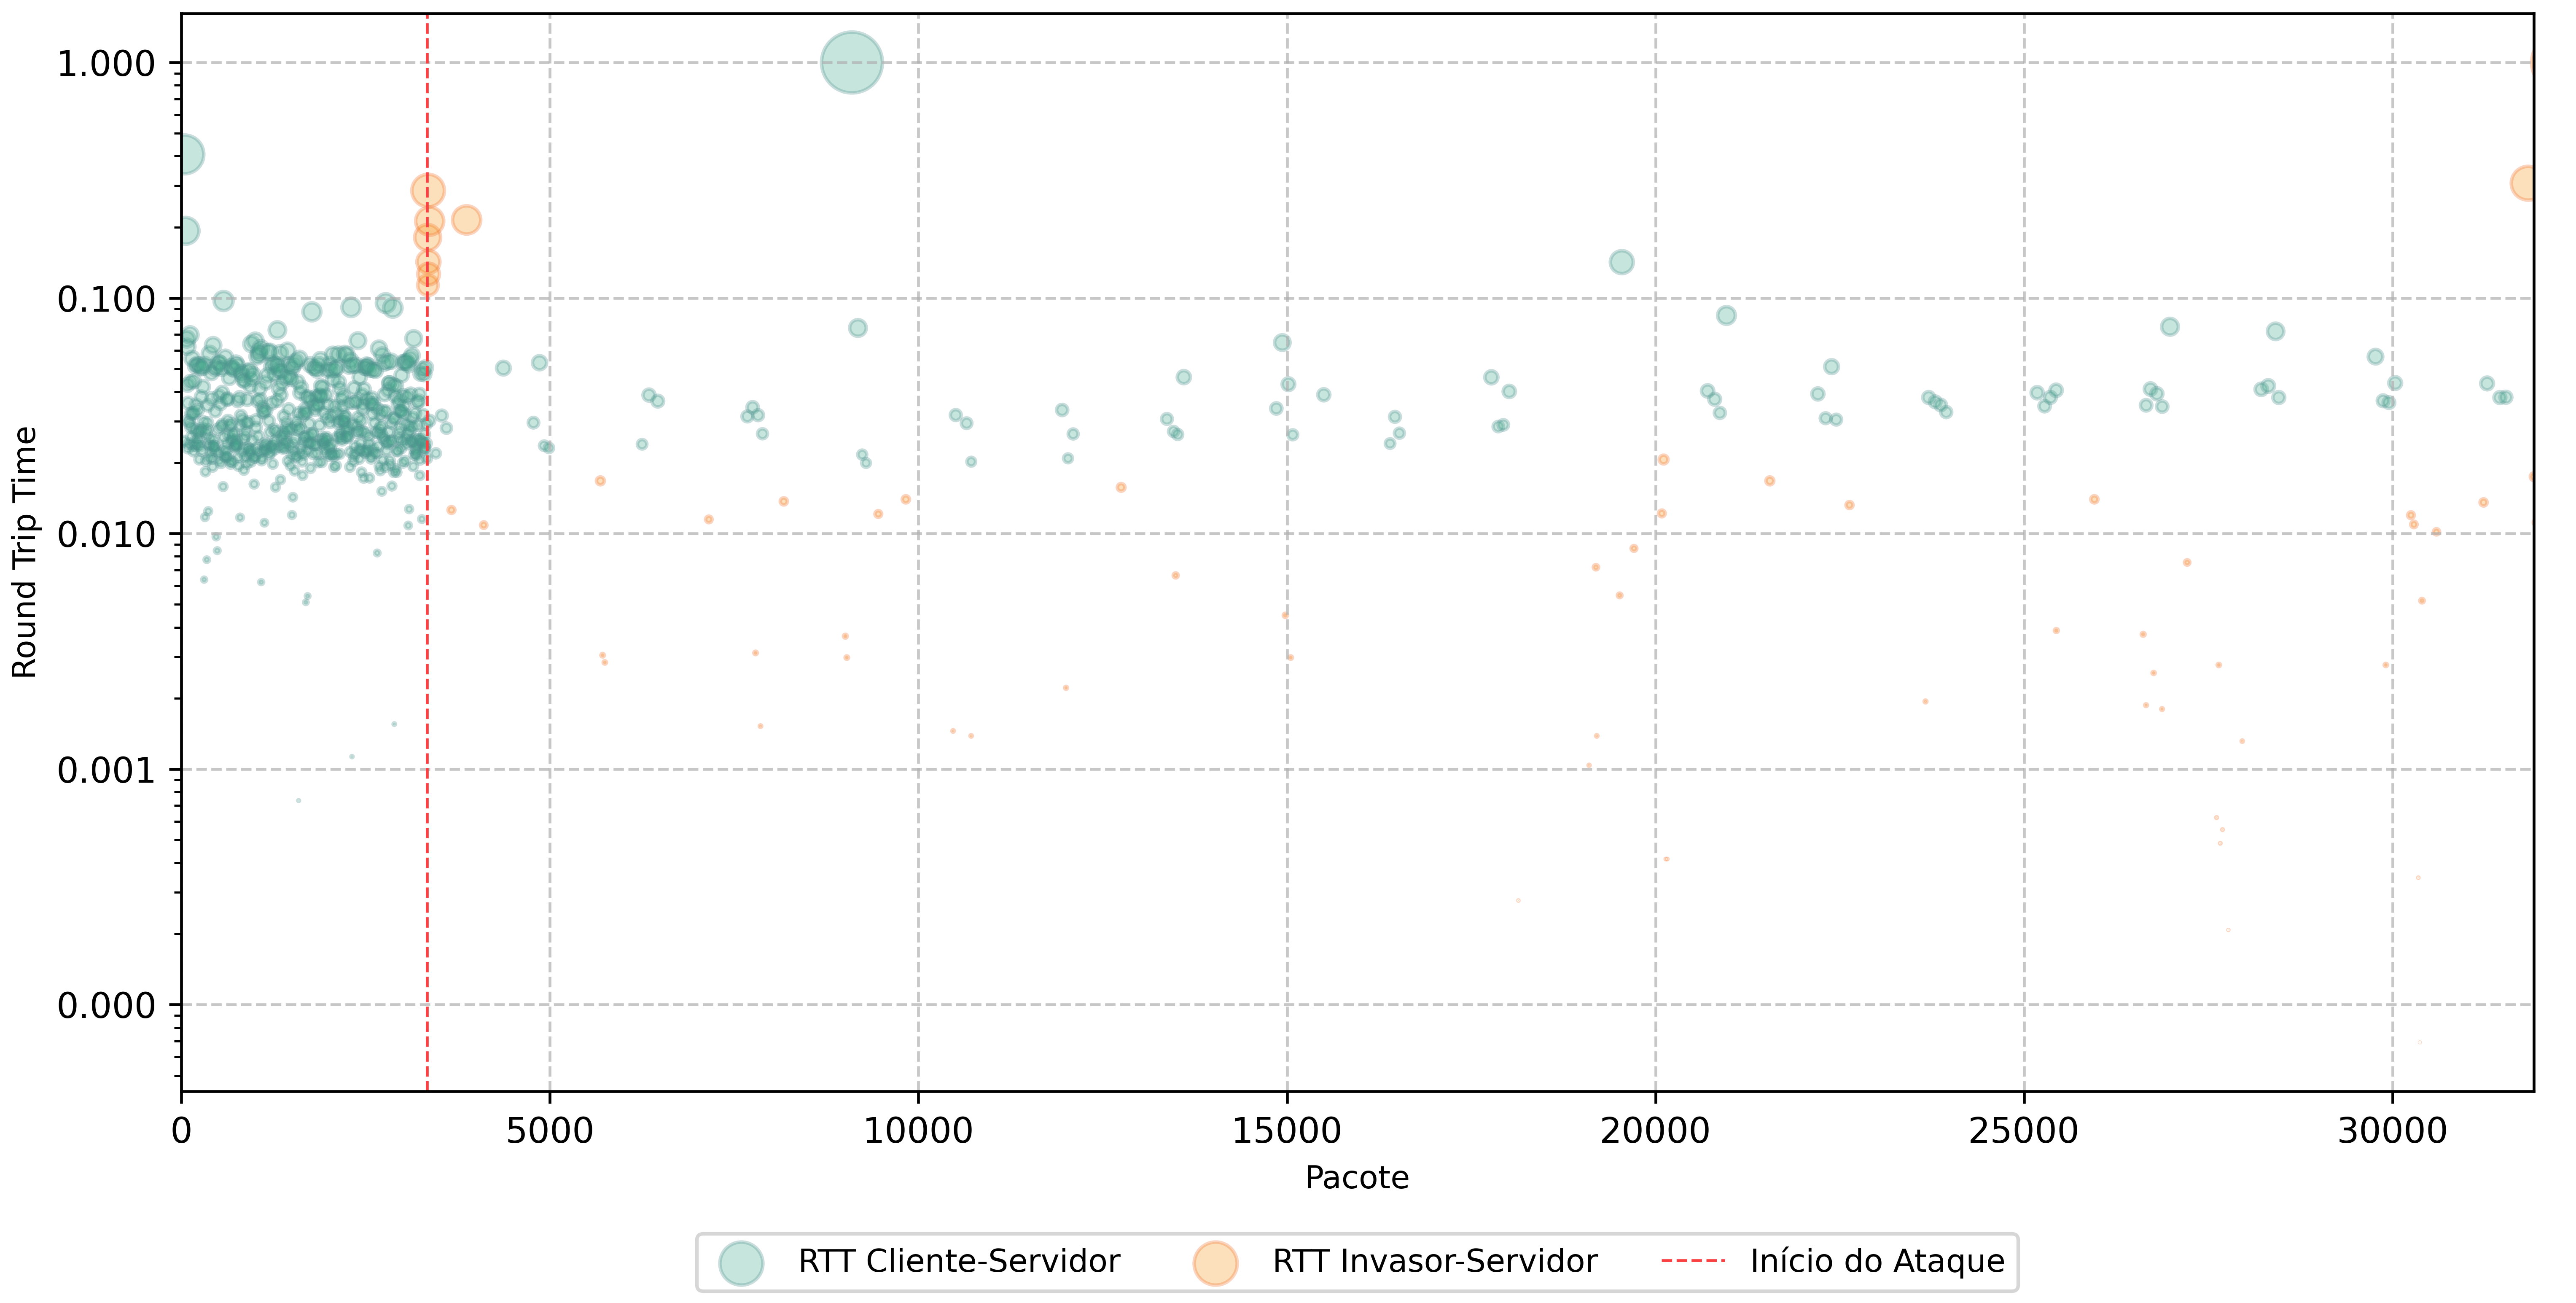
\includegraphics[width=1\textwidth, height=120pt]{USPSC-img/output/cropped/2-dos_function_call_null_deref-rttp.png}
        \caption{RTT por pacote}
    \end{subfigure}%
    % ~
    % \begin{subfigure}[t]{0.5\textwidth}
    %     \centering
    %     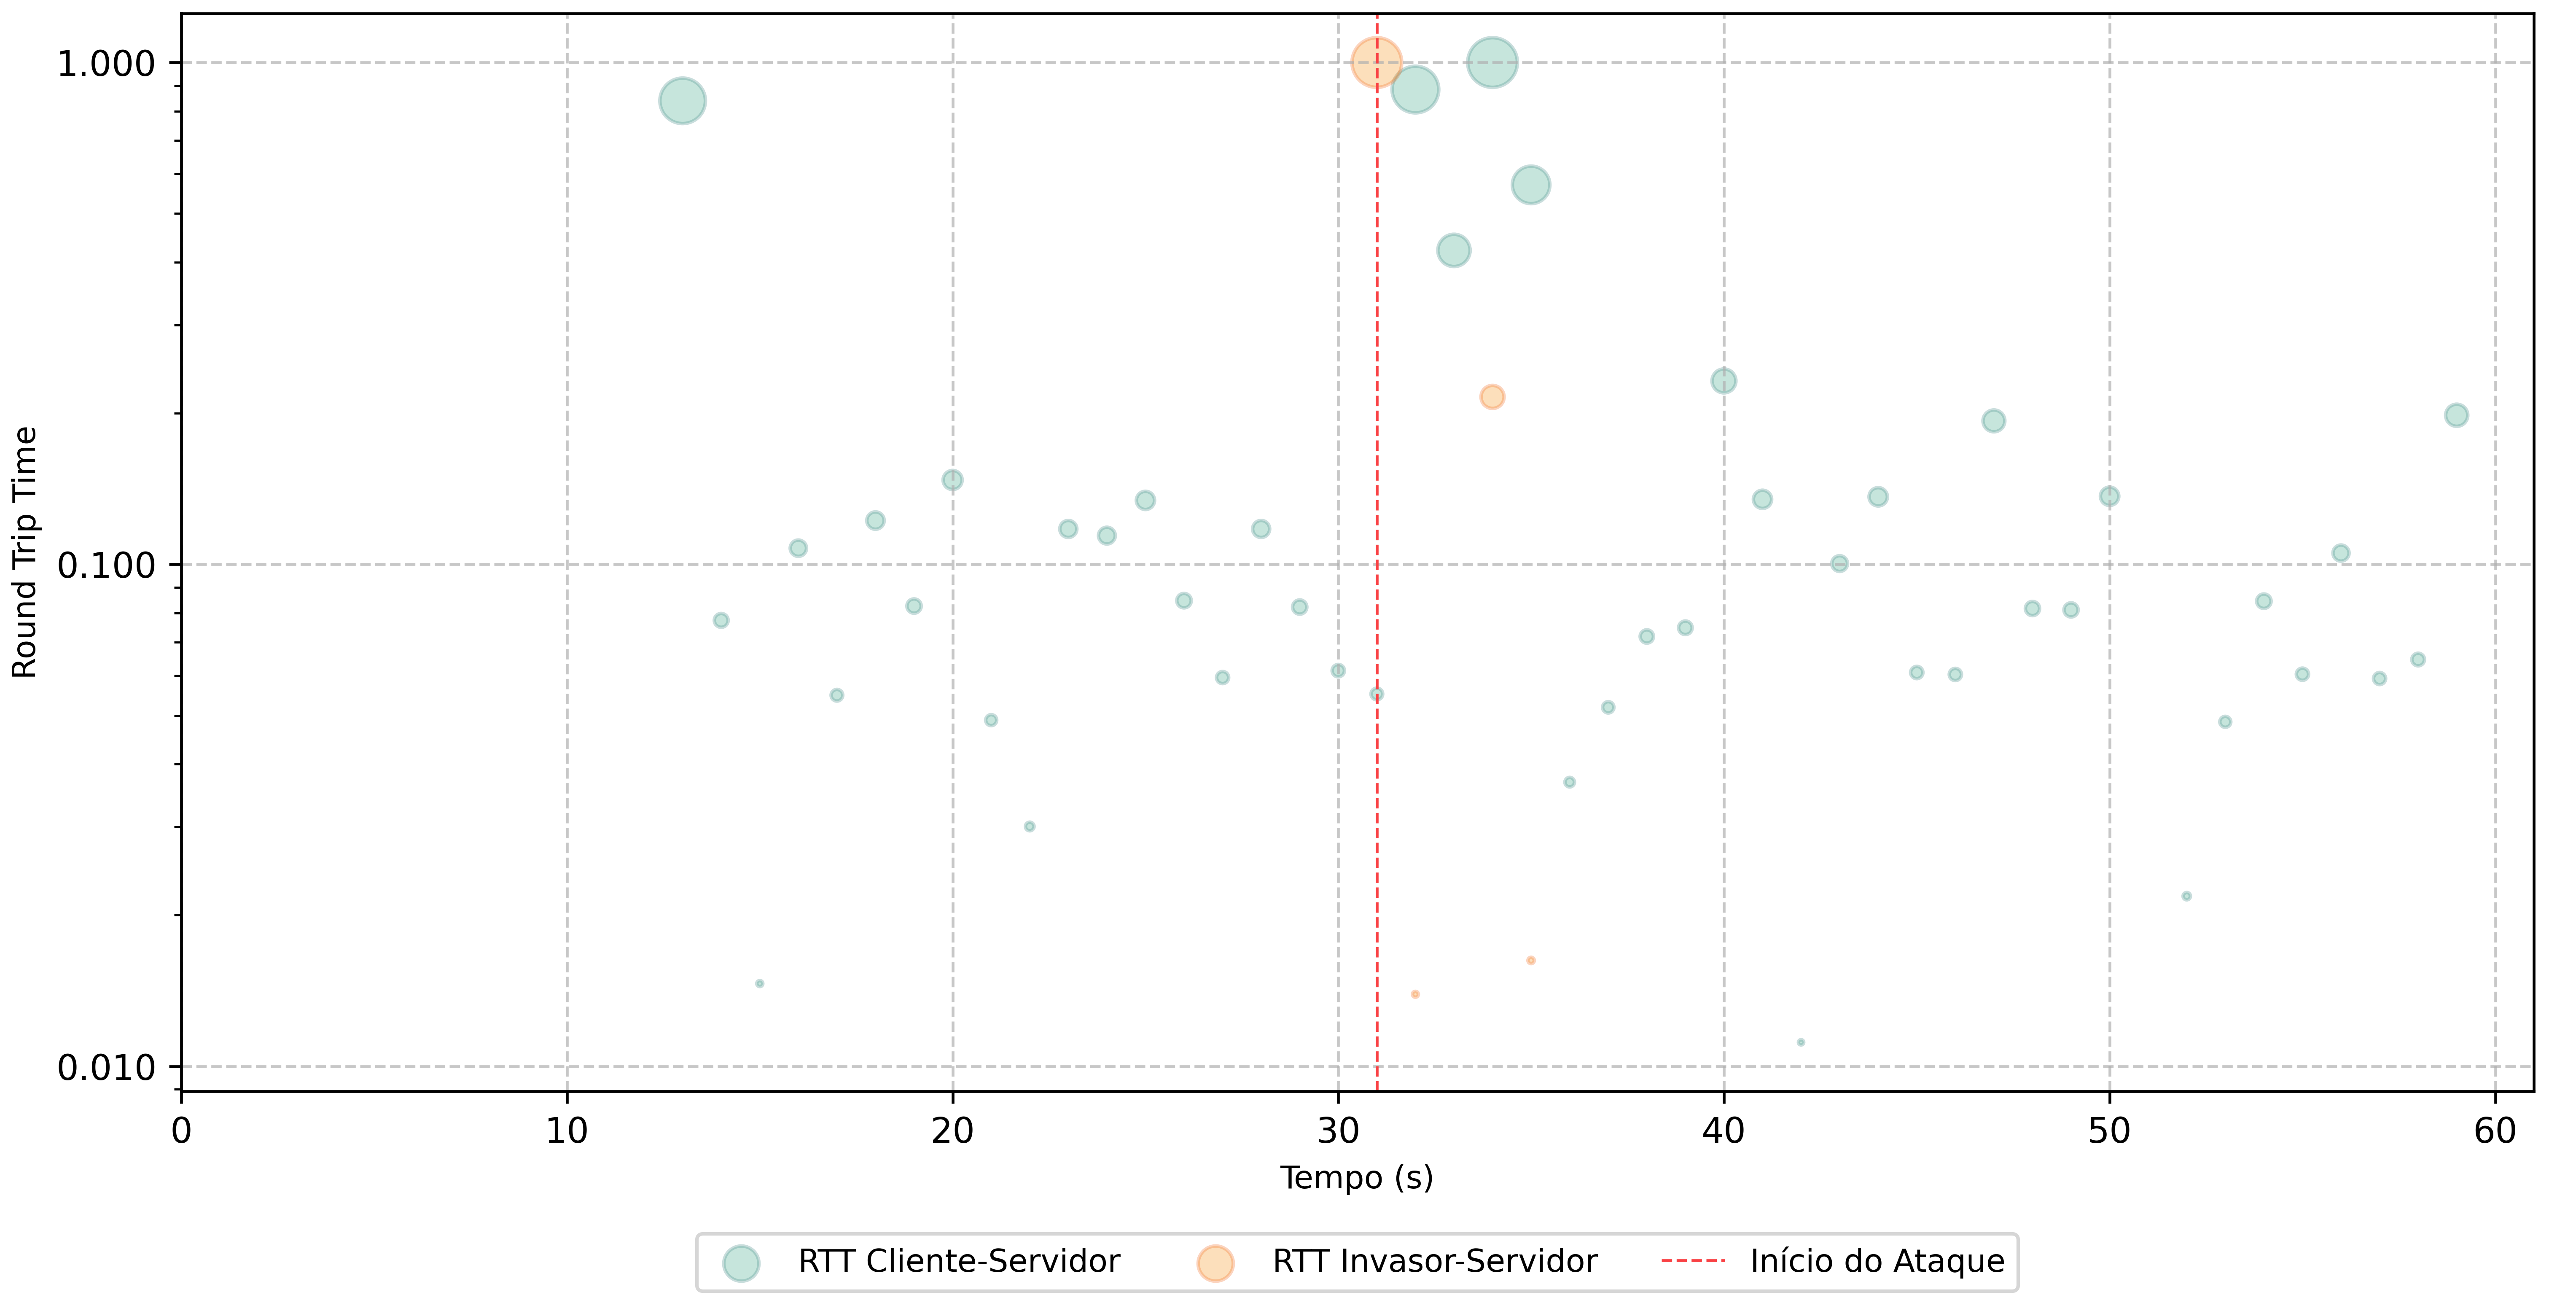
\includegraphics[width=1\textwidth, height=120pt]{USPSC-img/output/cropped/2-dos_function_call_null_deref-rtts.png}
    %     \caption{RTT por segundos}
    % \end{subfigure}%
    \label{fig:2-dos_function_call_null_deref}
    \caption{Gráficos do ataque de DoS pela chamada da função \textit{Dereference} nula - nível de segurança: `Sign \& Encrypt'.}
\end{figure}

\begin{figure}[htbp!]
    \centering
    \begin{subfigure}[t]{0.5\textwidth}
        \centering
        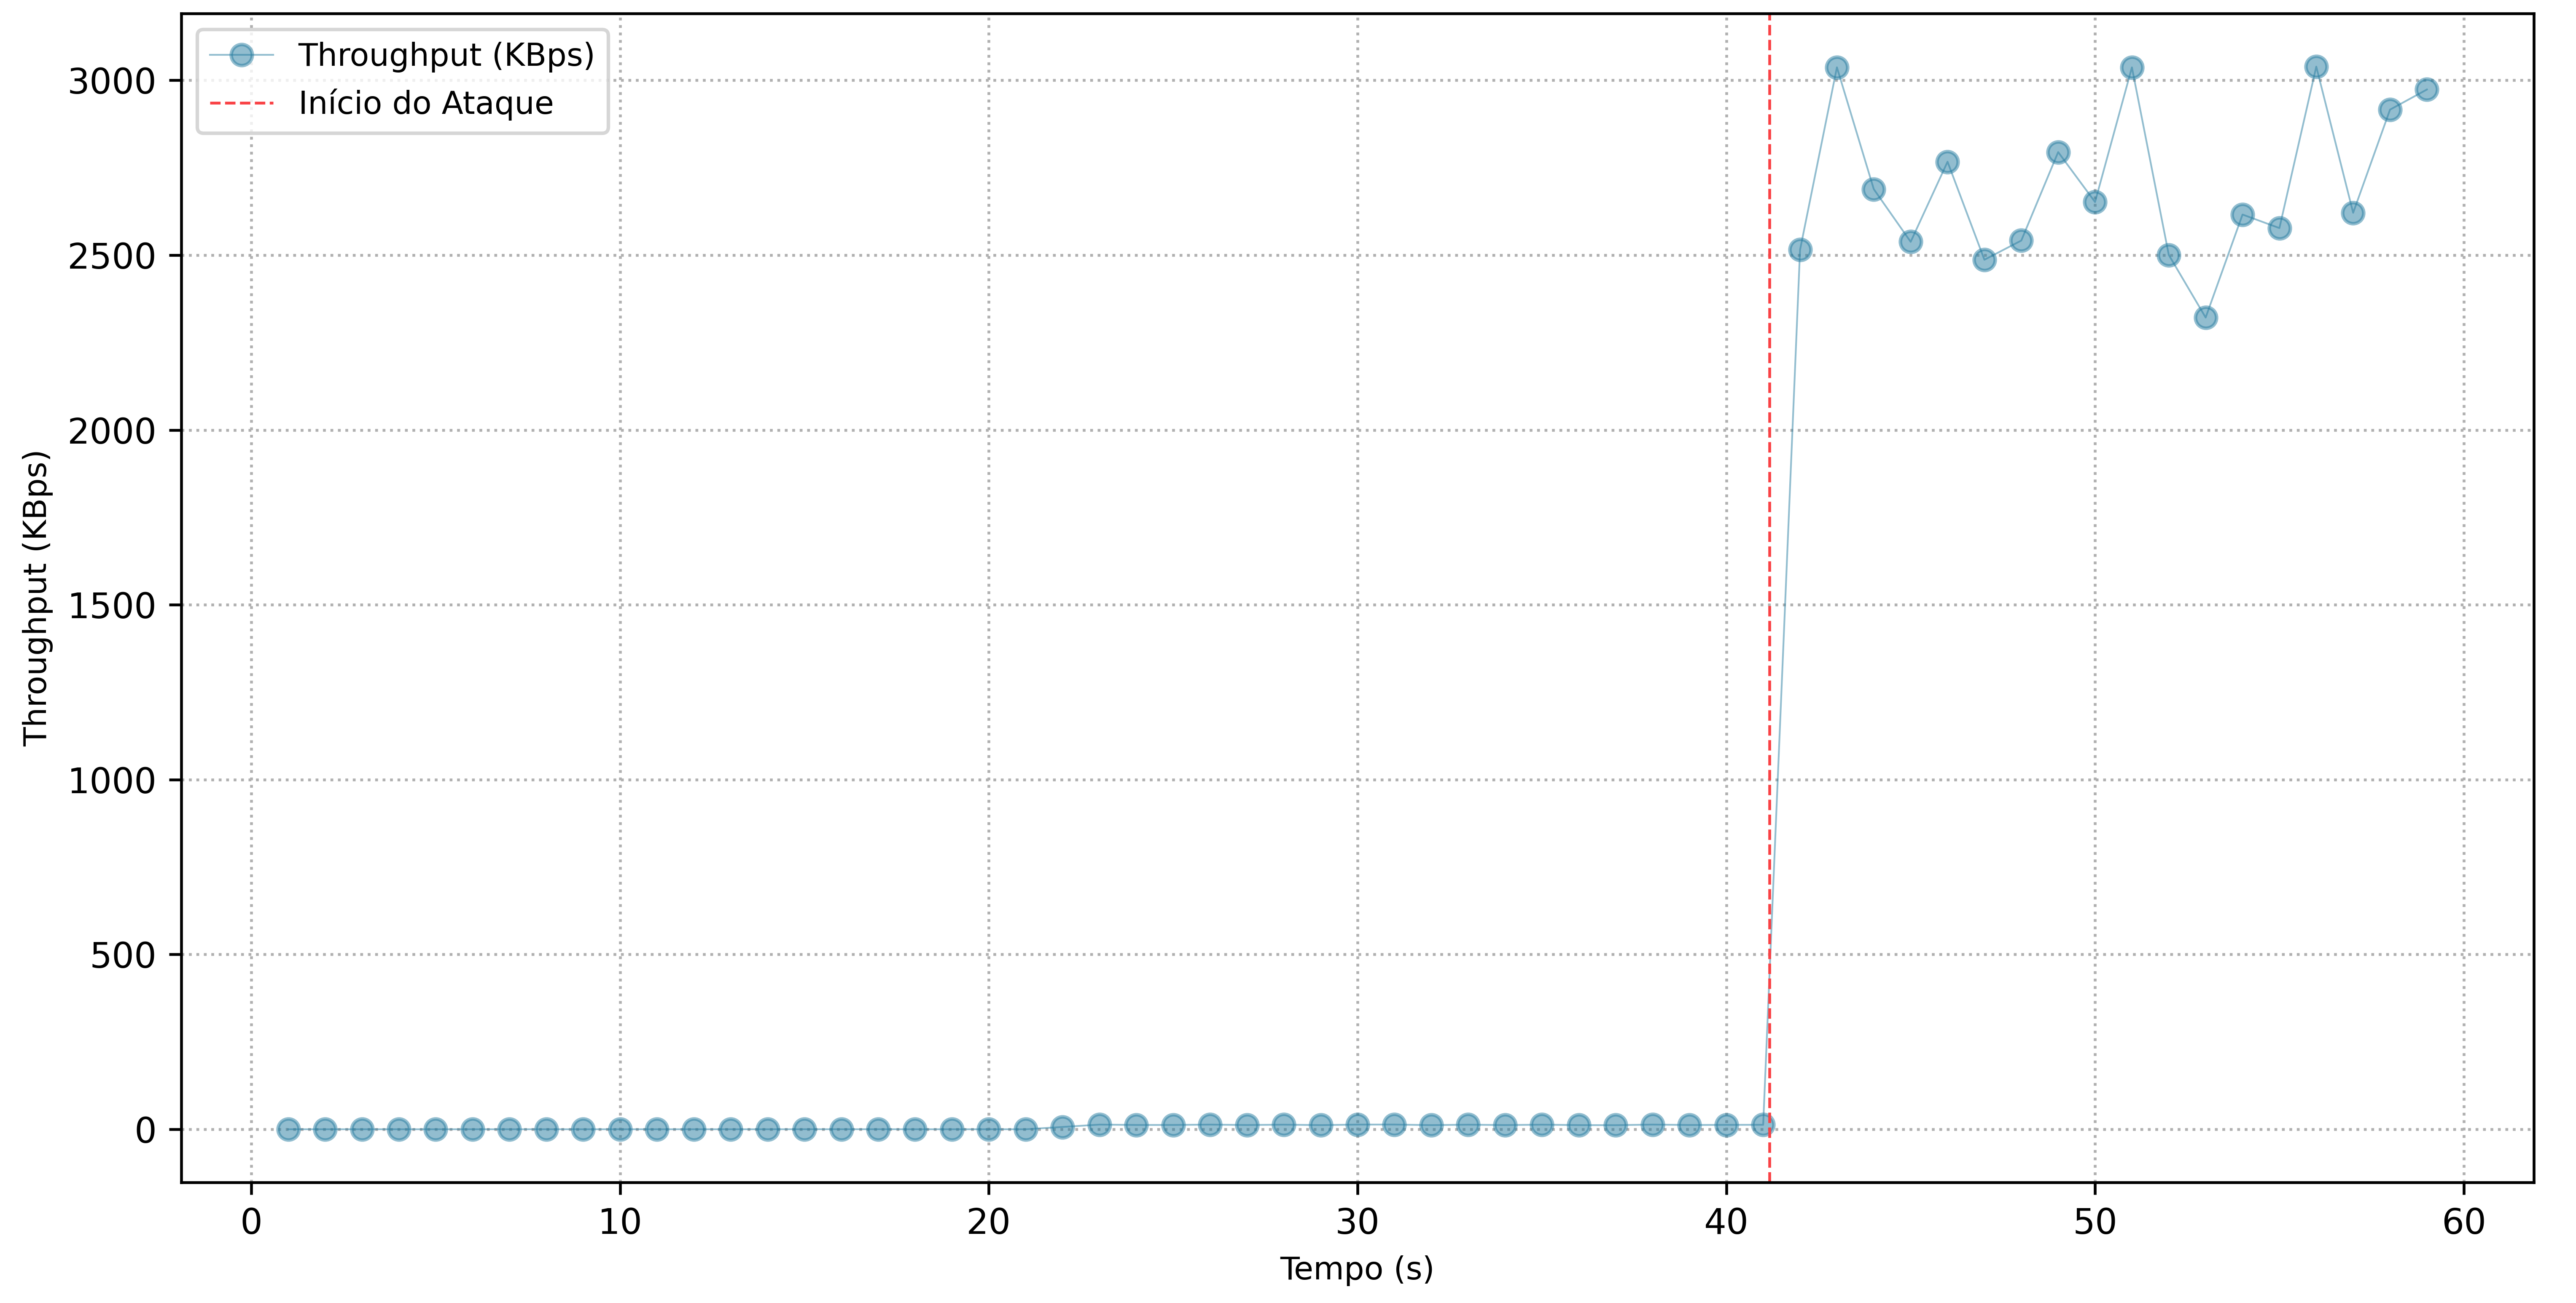
\includegraphics[width=1\textwidth, height=120pt]{USPSC-img/output/cropped/0-dos_hping3-tput.png}
        \caption{\textit{Throughput}}
    \end{subfigure}%
    ~ 
    \begin{subfigure}[t]{0.5\textwidth}
        \centering
        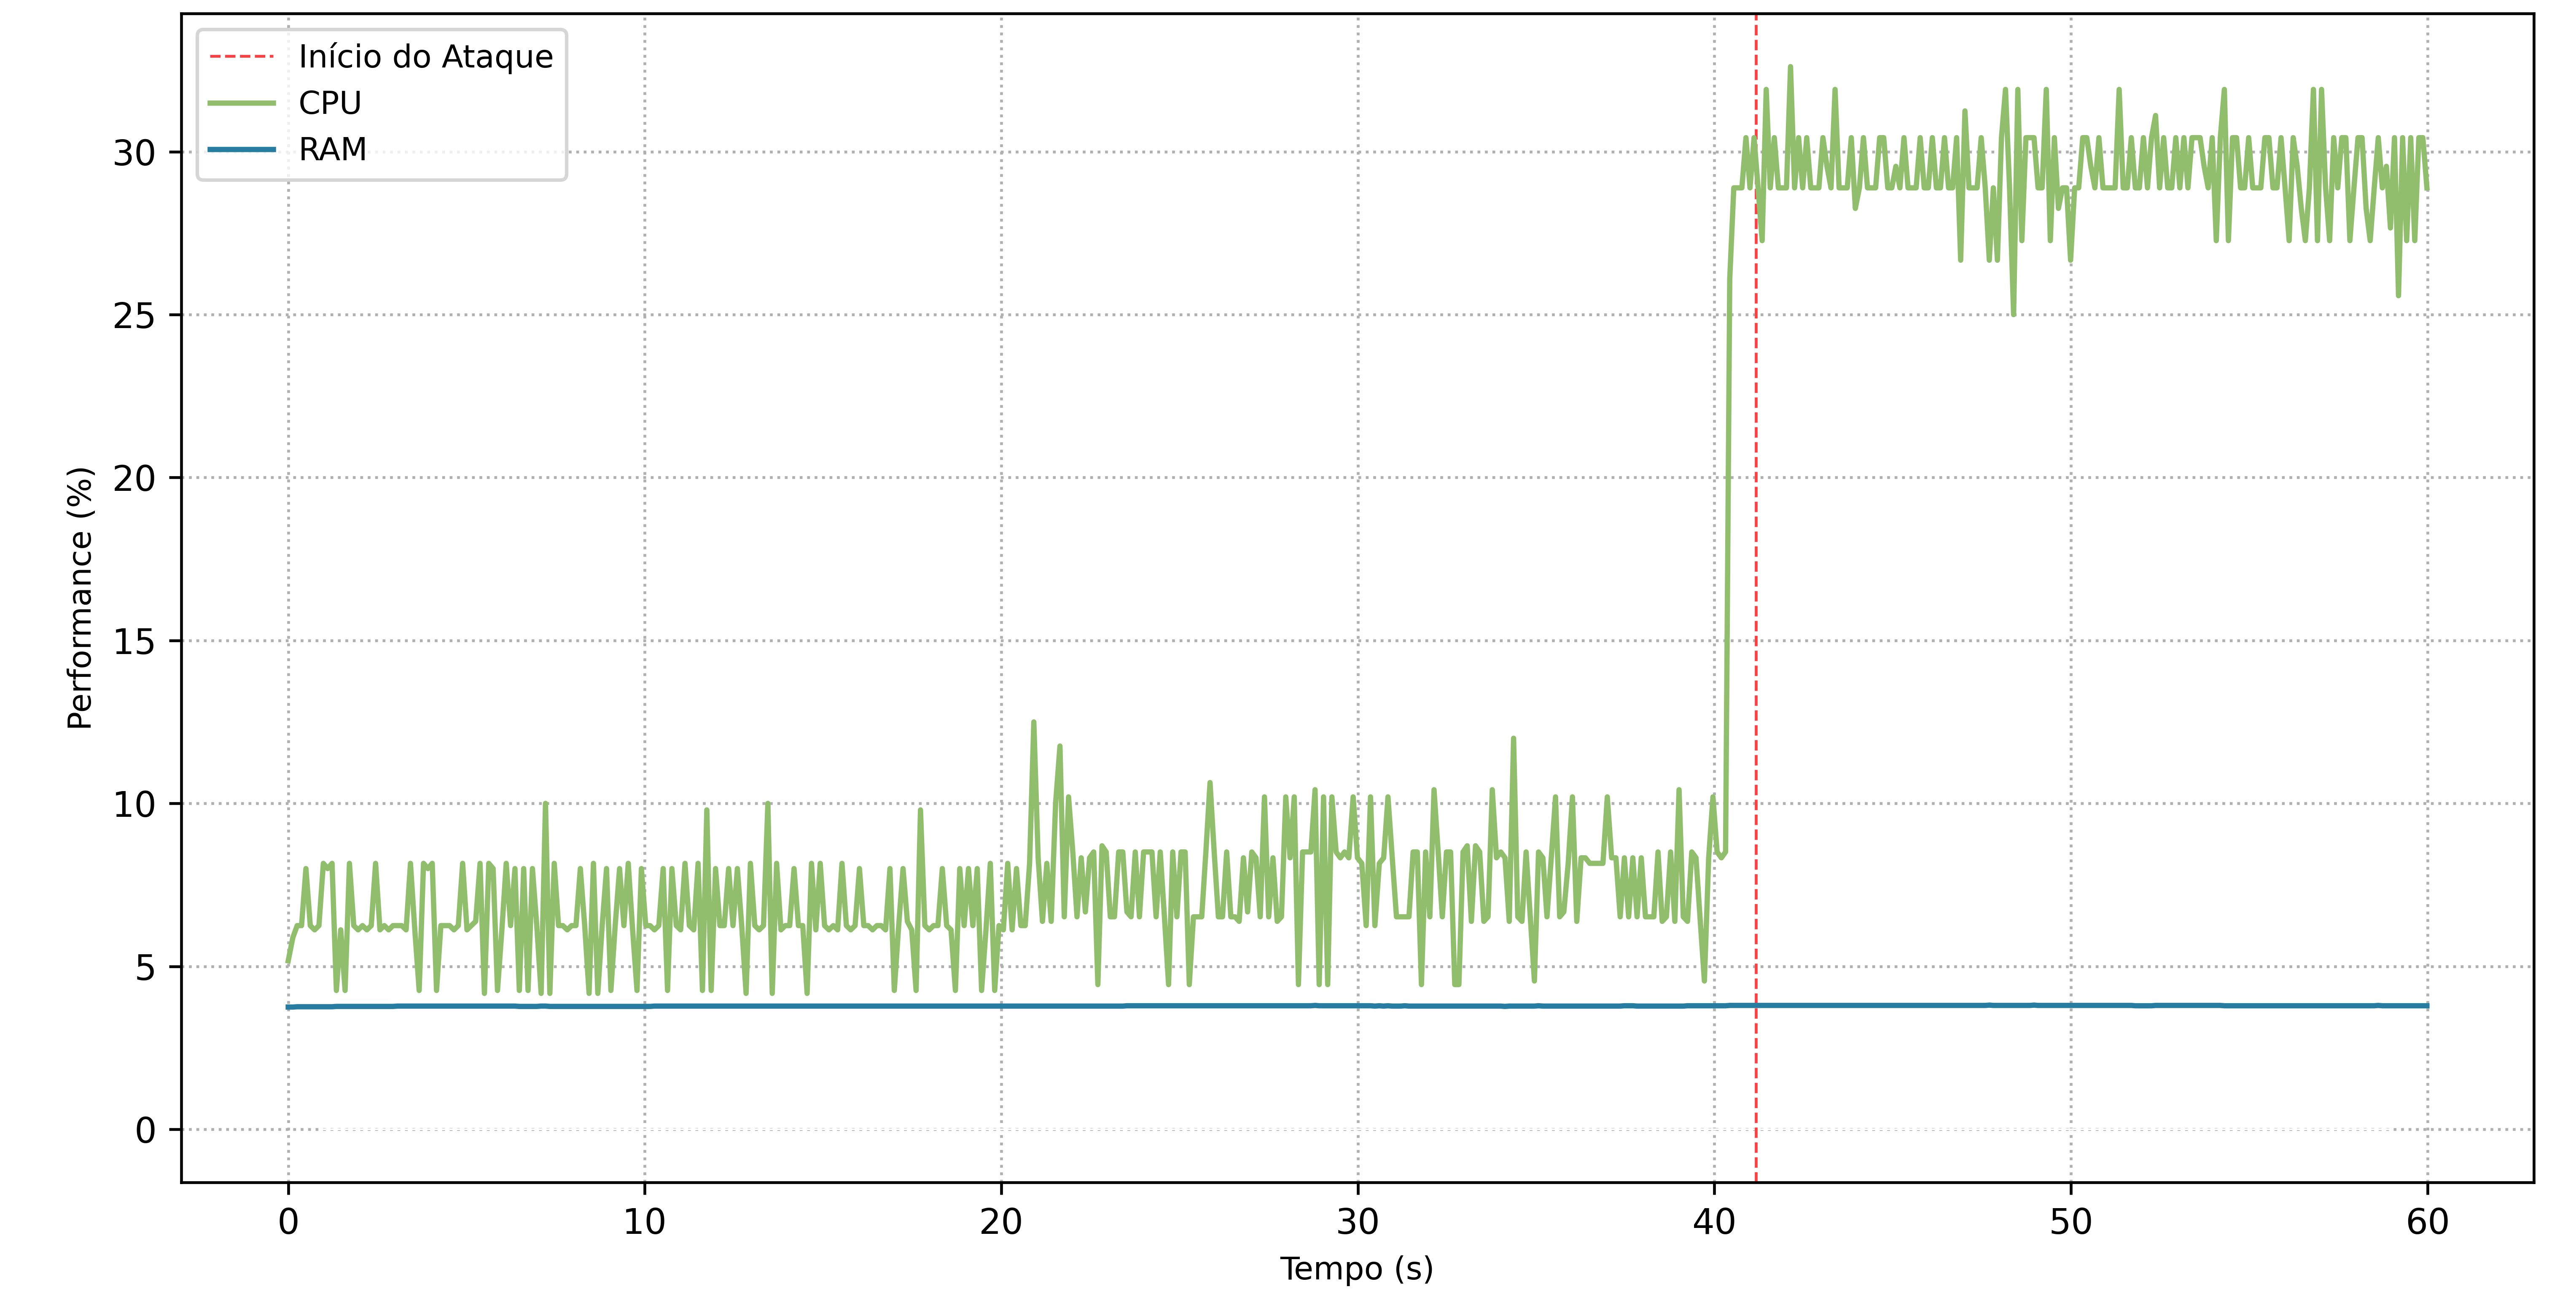
\includegraphics[width=1\textwidth, height=120pt]{USPSC-img/output/cropped/0-dos_hping3-perf.png}
        \caption{Desempenho}
    \end{subfigure}%
    \\
    \begin{subfigure}[t]{0.5\textwidth}
        \centering
        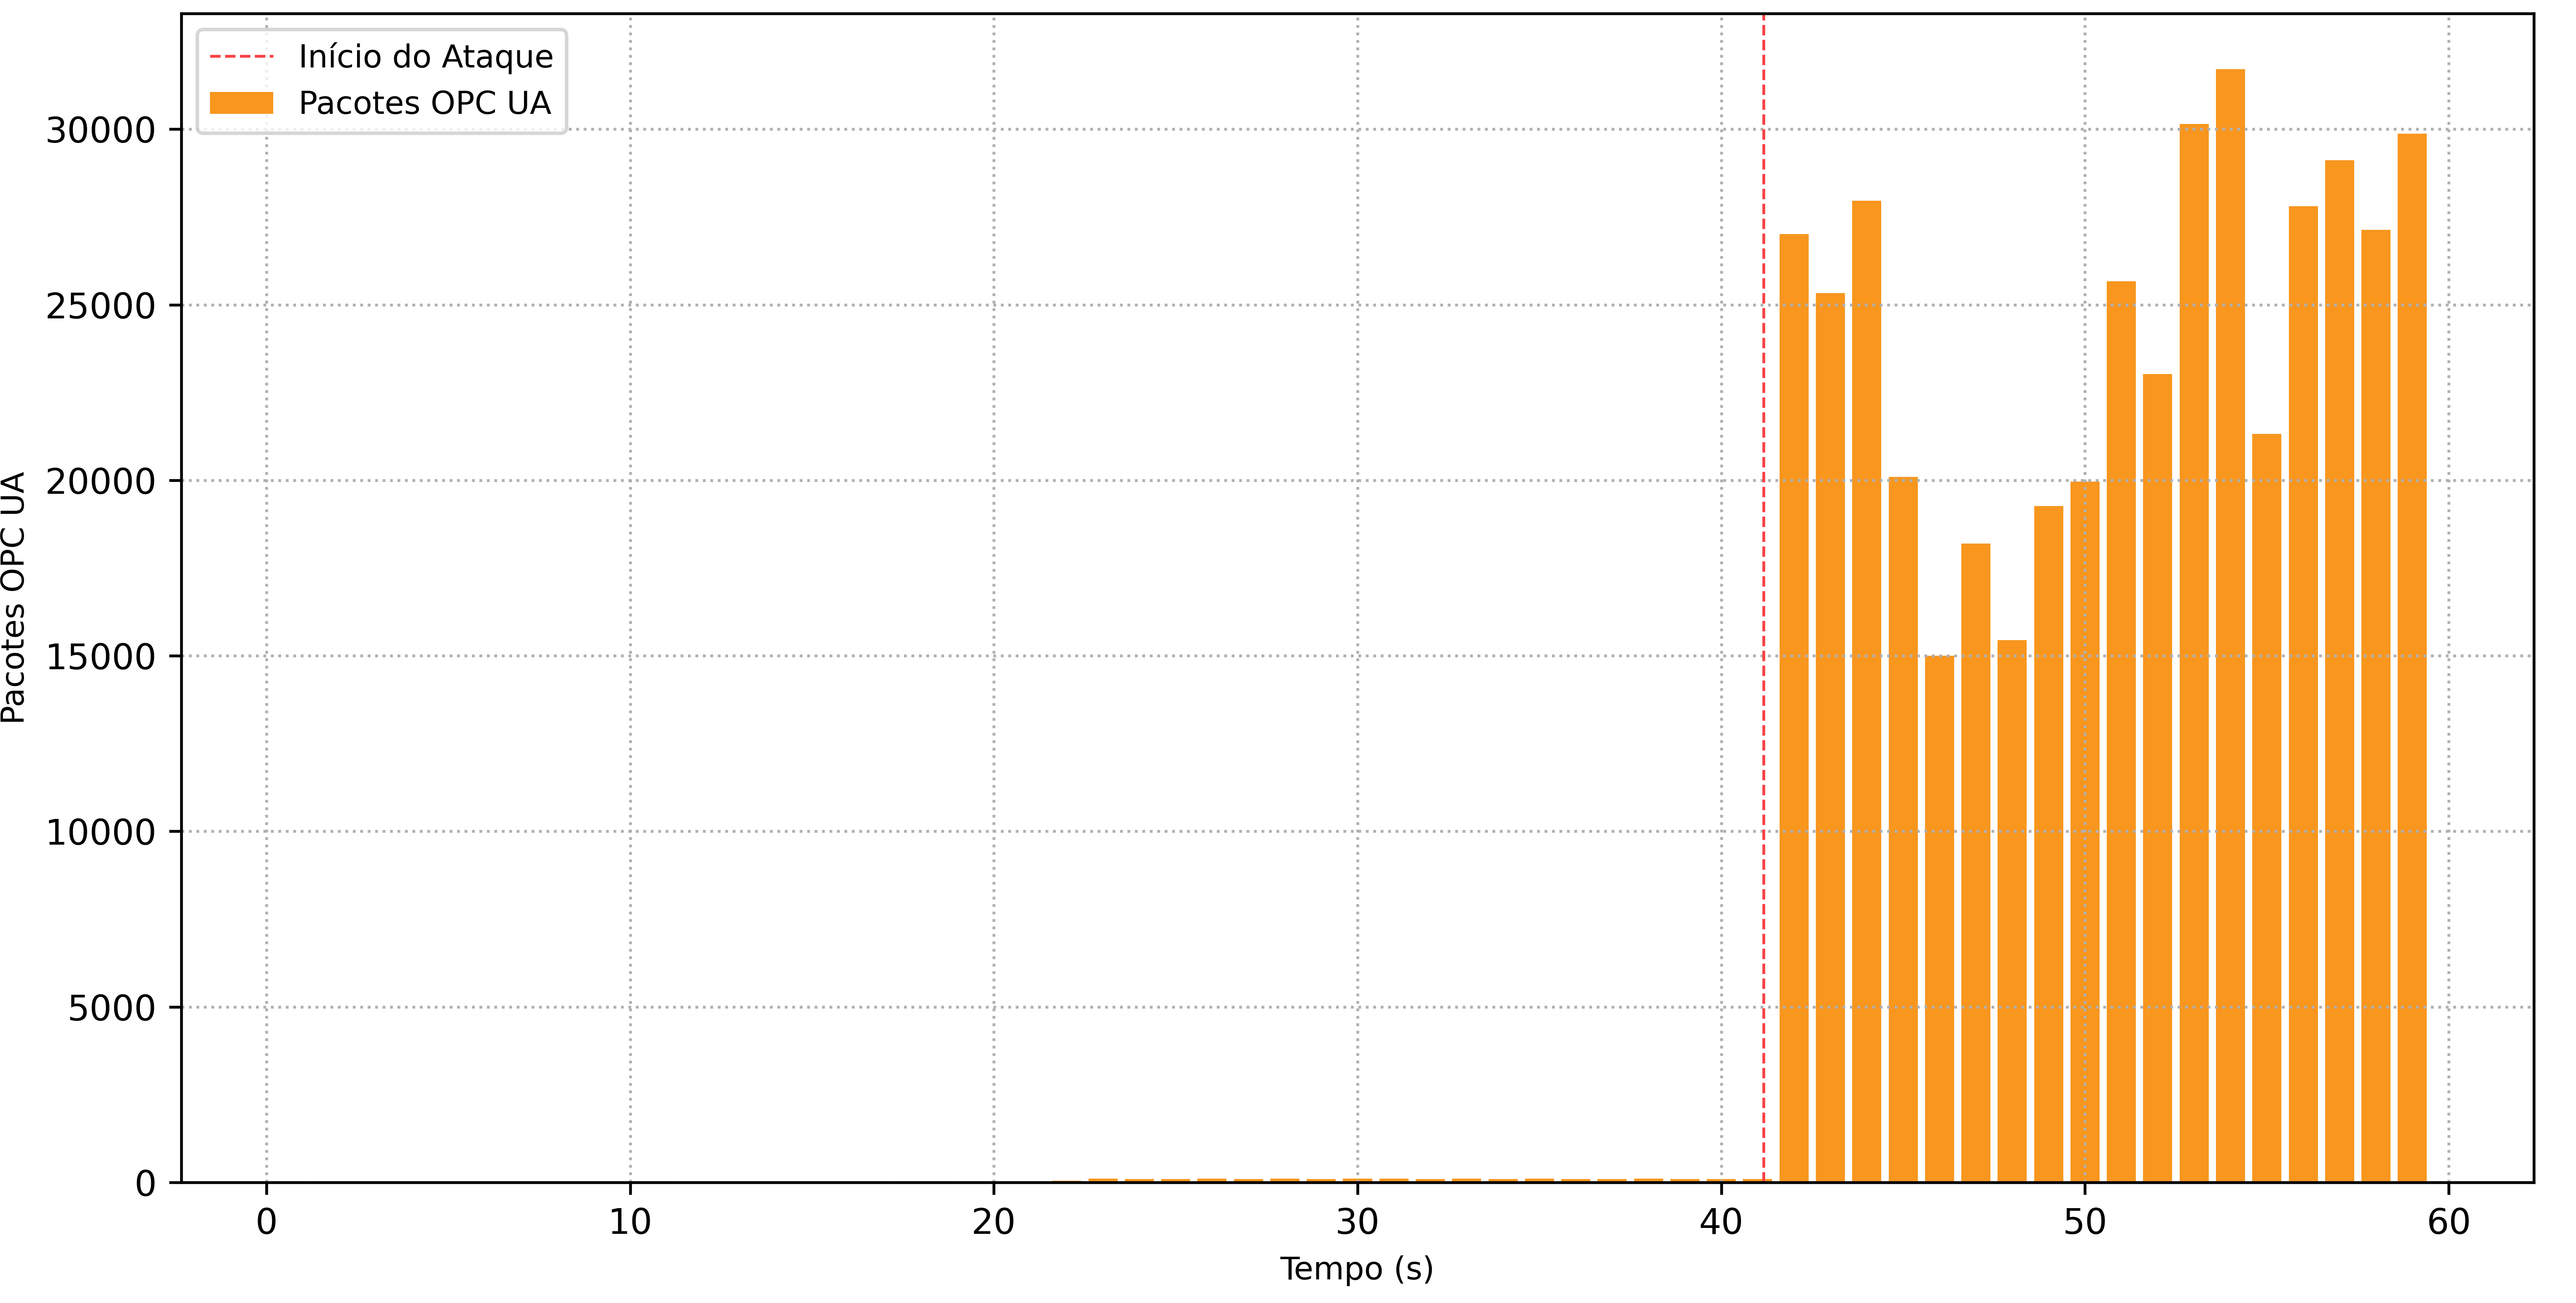
\includegraphics[width=1\textwidth, height=120pt]{USPSC-img/output/cropped/0-dos_hping3-pack.png}
        \caption{Pacotes OPC UA}
    \end{subfigure}%
    ~
    \begin{subfigure}[t]{0.5\textwidth}
        \centering
        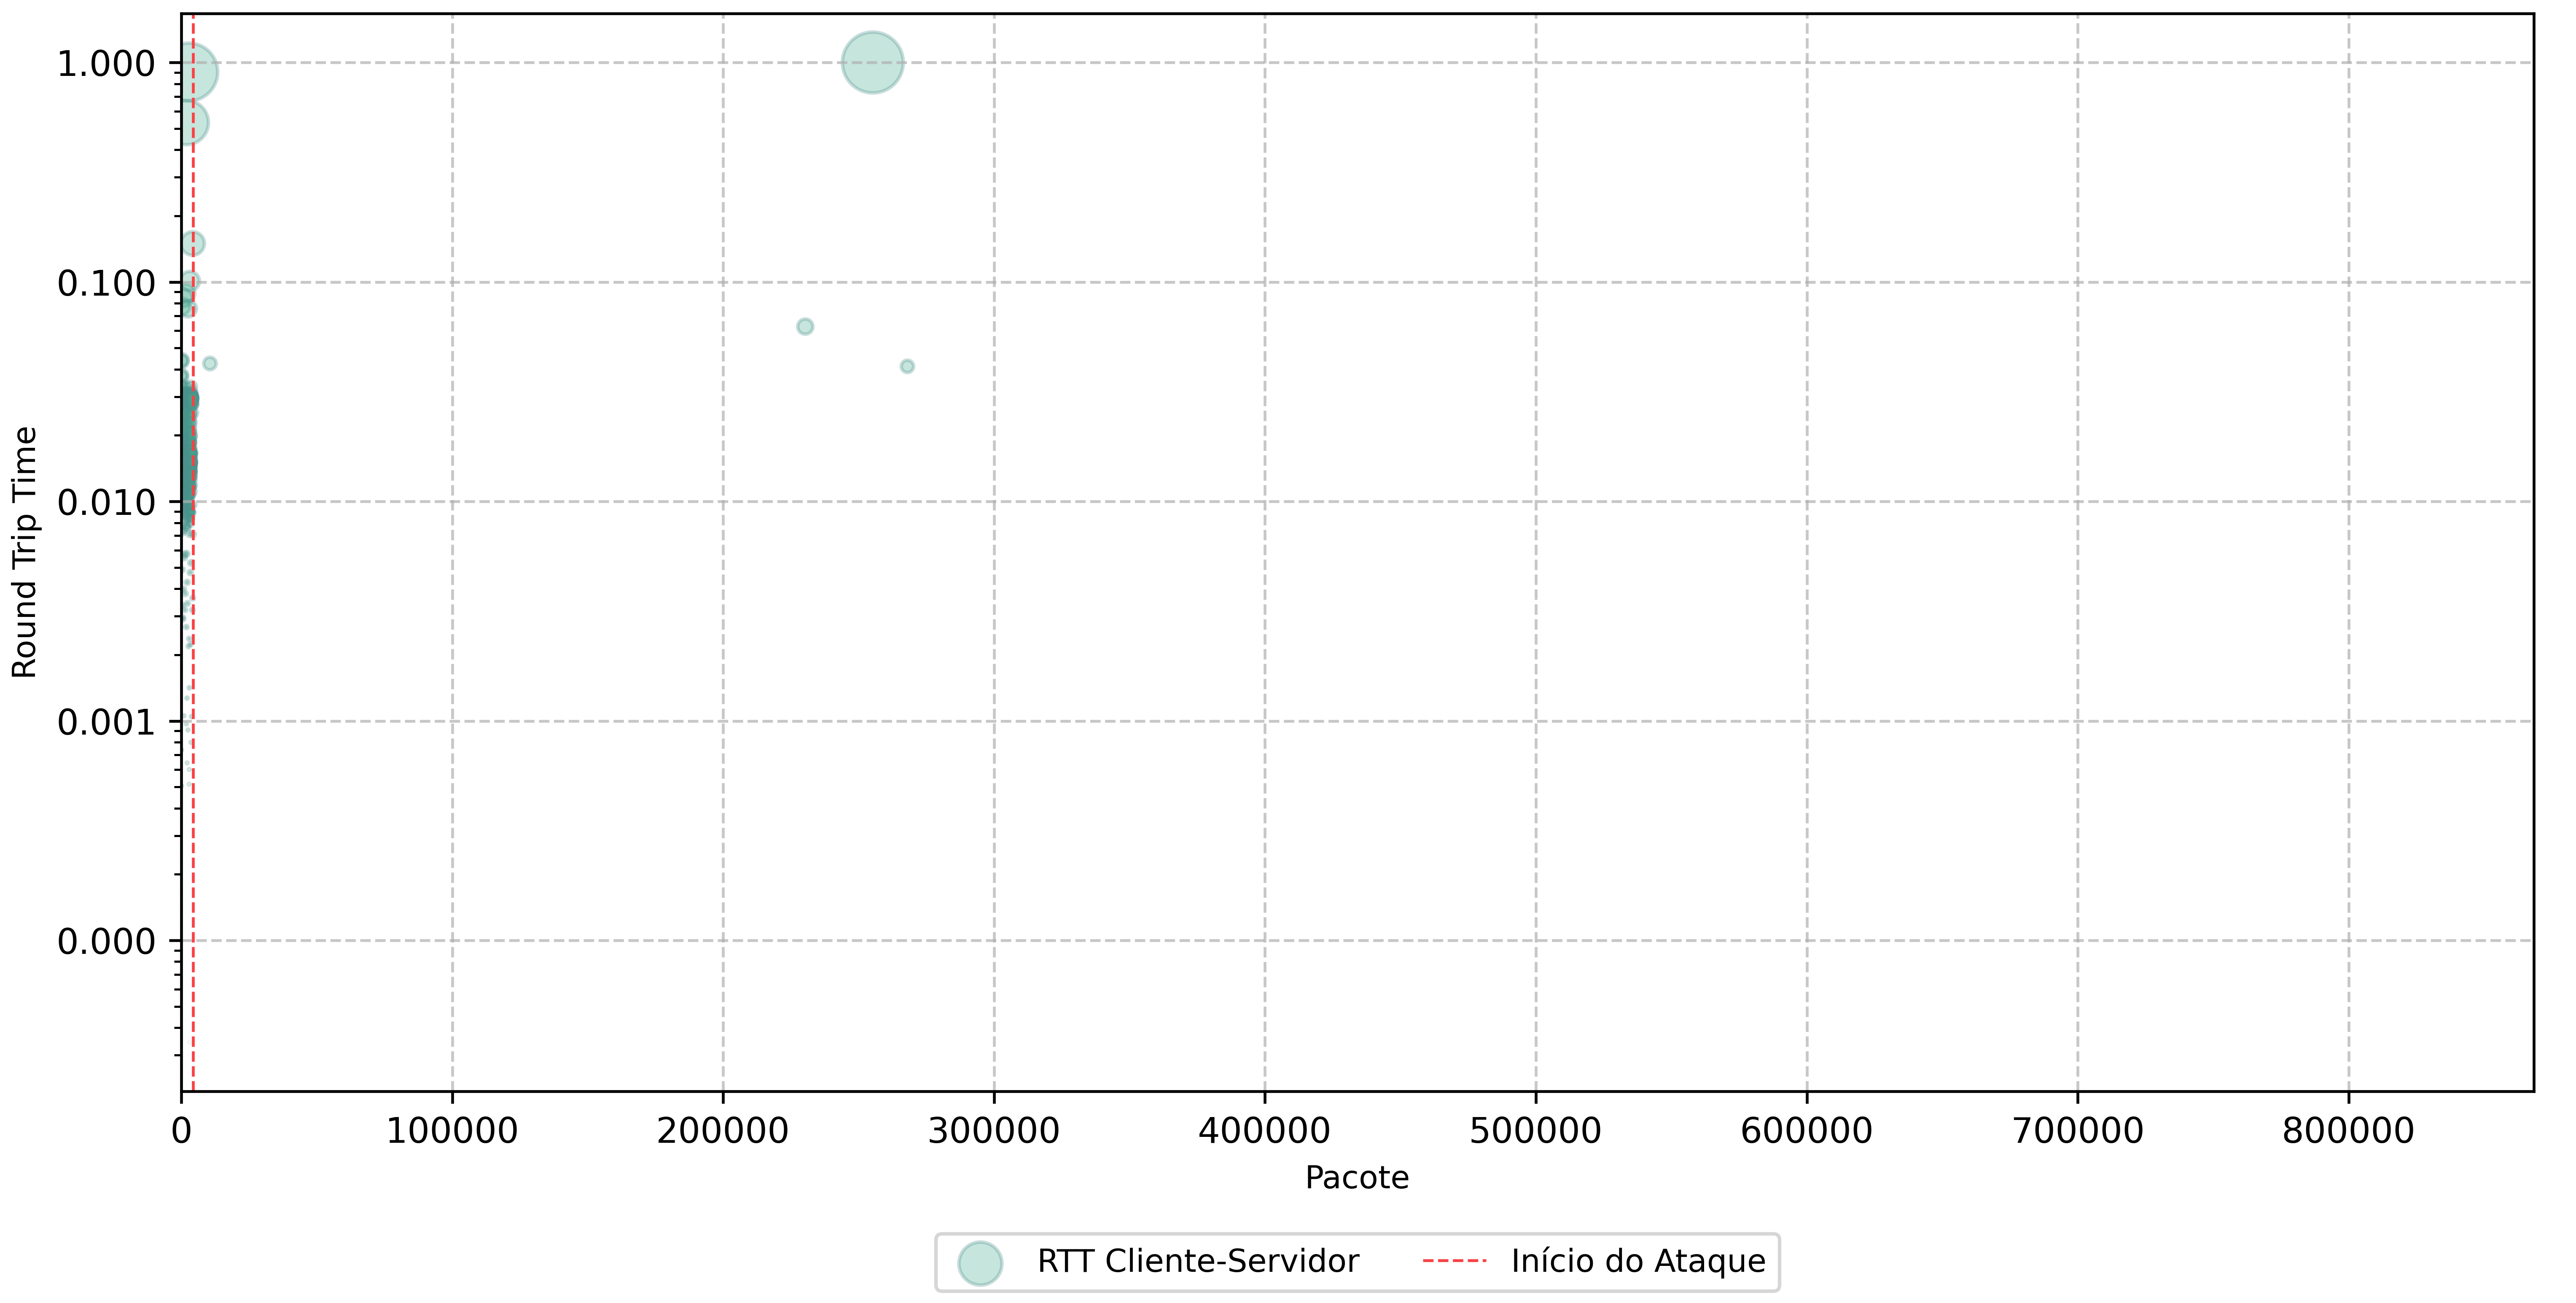
\includegraphics[width=1\textwidth, height=120pt]{USPSC-img/output/cropped/0-dos_hping3-rttp.png}
        \caption{RTT por pacote}
    \end{subfigure}%
    % ~
    % \begin{subfigure}[t]{0.5\textwidth}
    %     \centering
    %     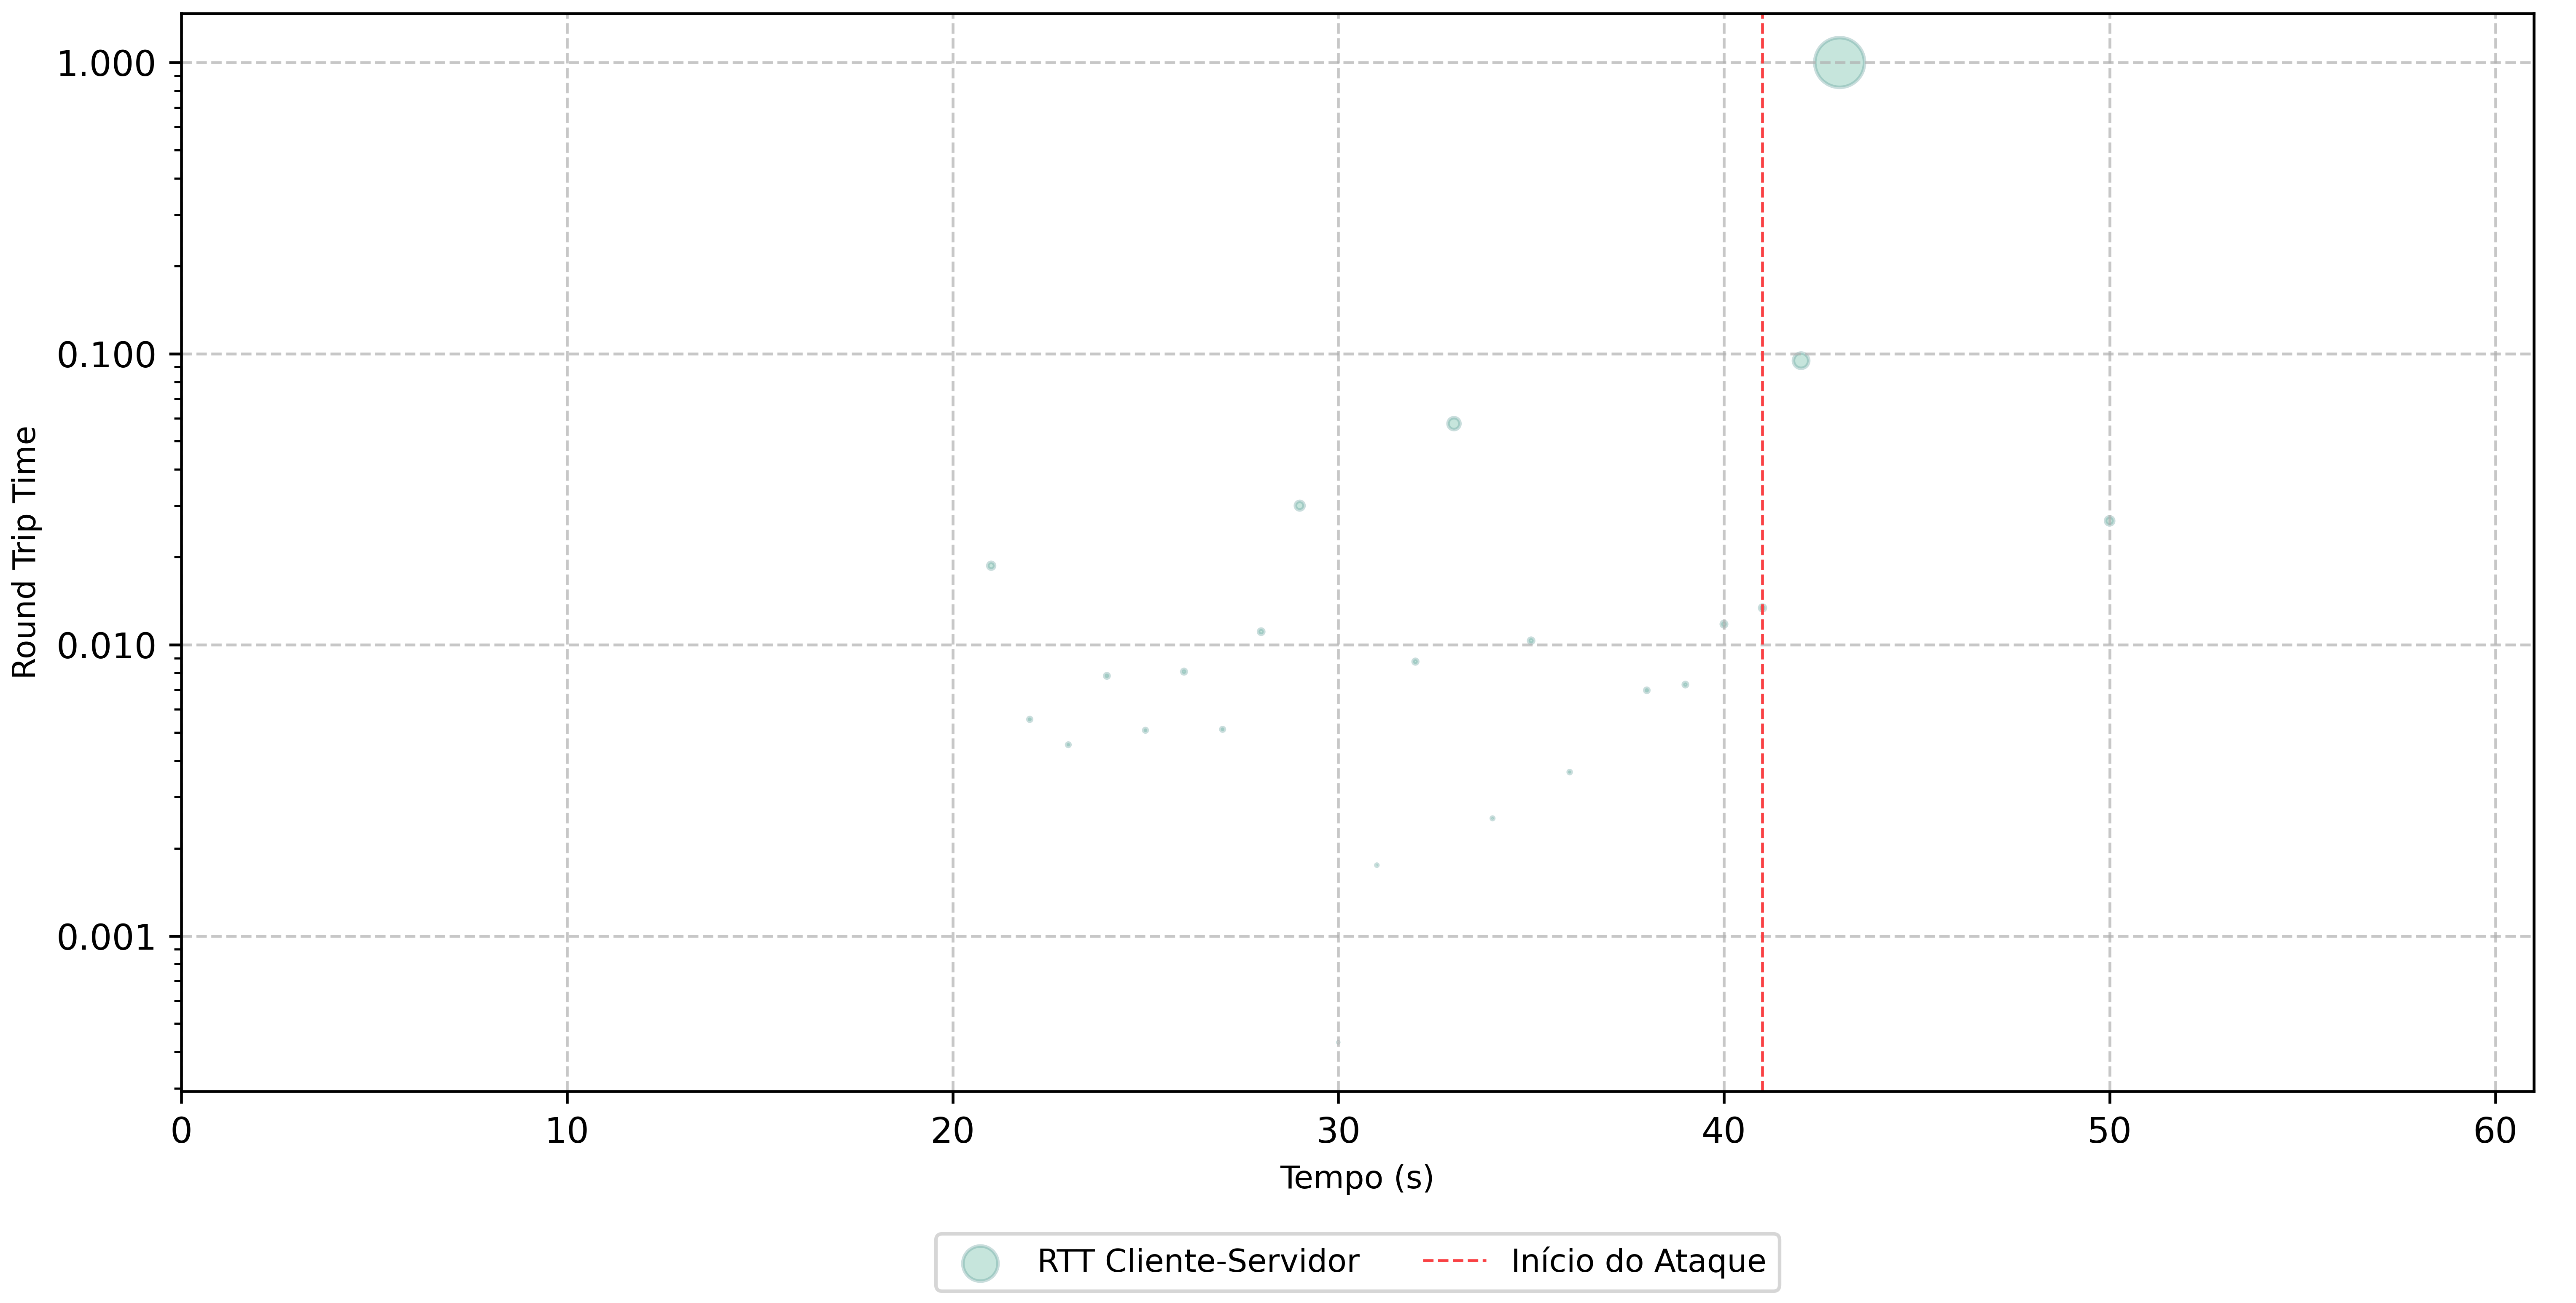
\includegraphics[width=1\textwidth, height=120pt]{USPSC-img/output/cropped/0-dos_hping3-rtts.png}
    %     \caption{RTT por segundos}
    % \end{subfigure}%
    \label{fig:0-dos_hping3}
    \caption{Gráficos do ataque de DoS por inundação TCP/IP - nível de segurança: `None'.}
\end{figure}

\begin{figure}[htbp!]
    \centering
    \begin{subfigure}[t]{0.5\textwidth}
        \centering
        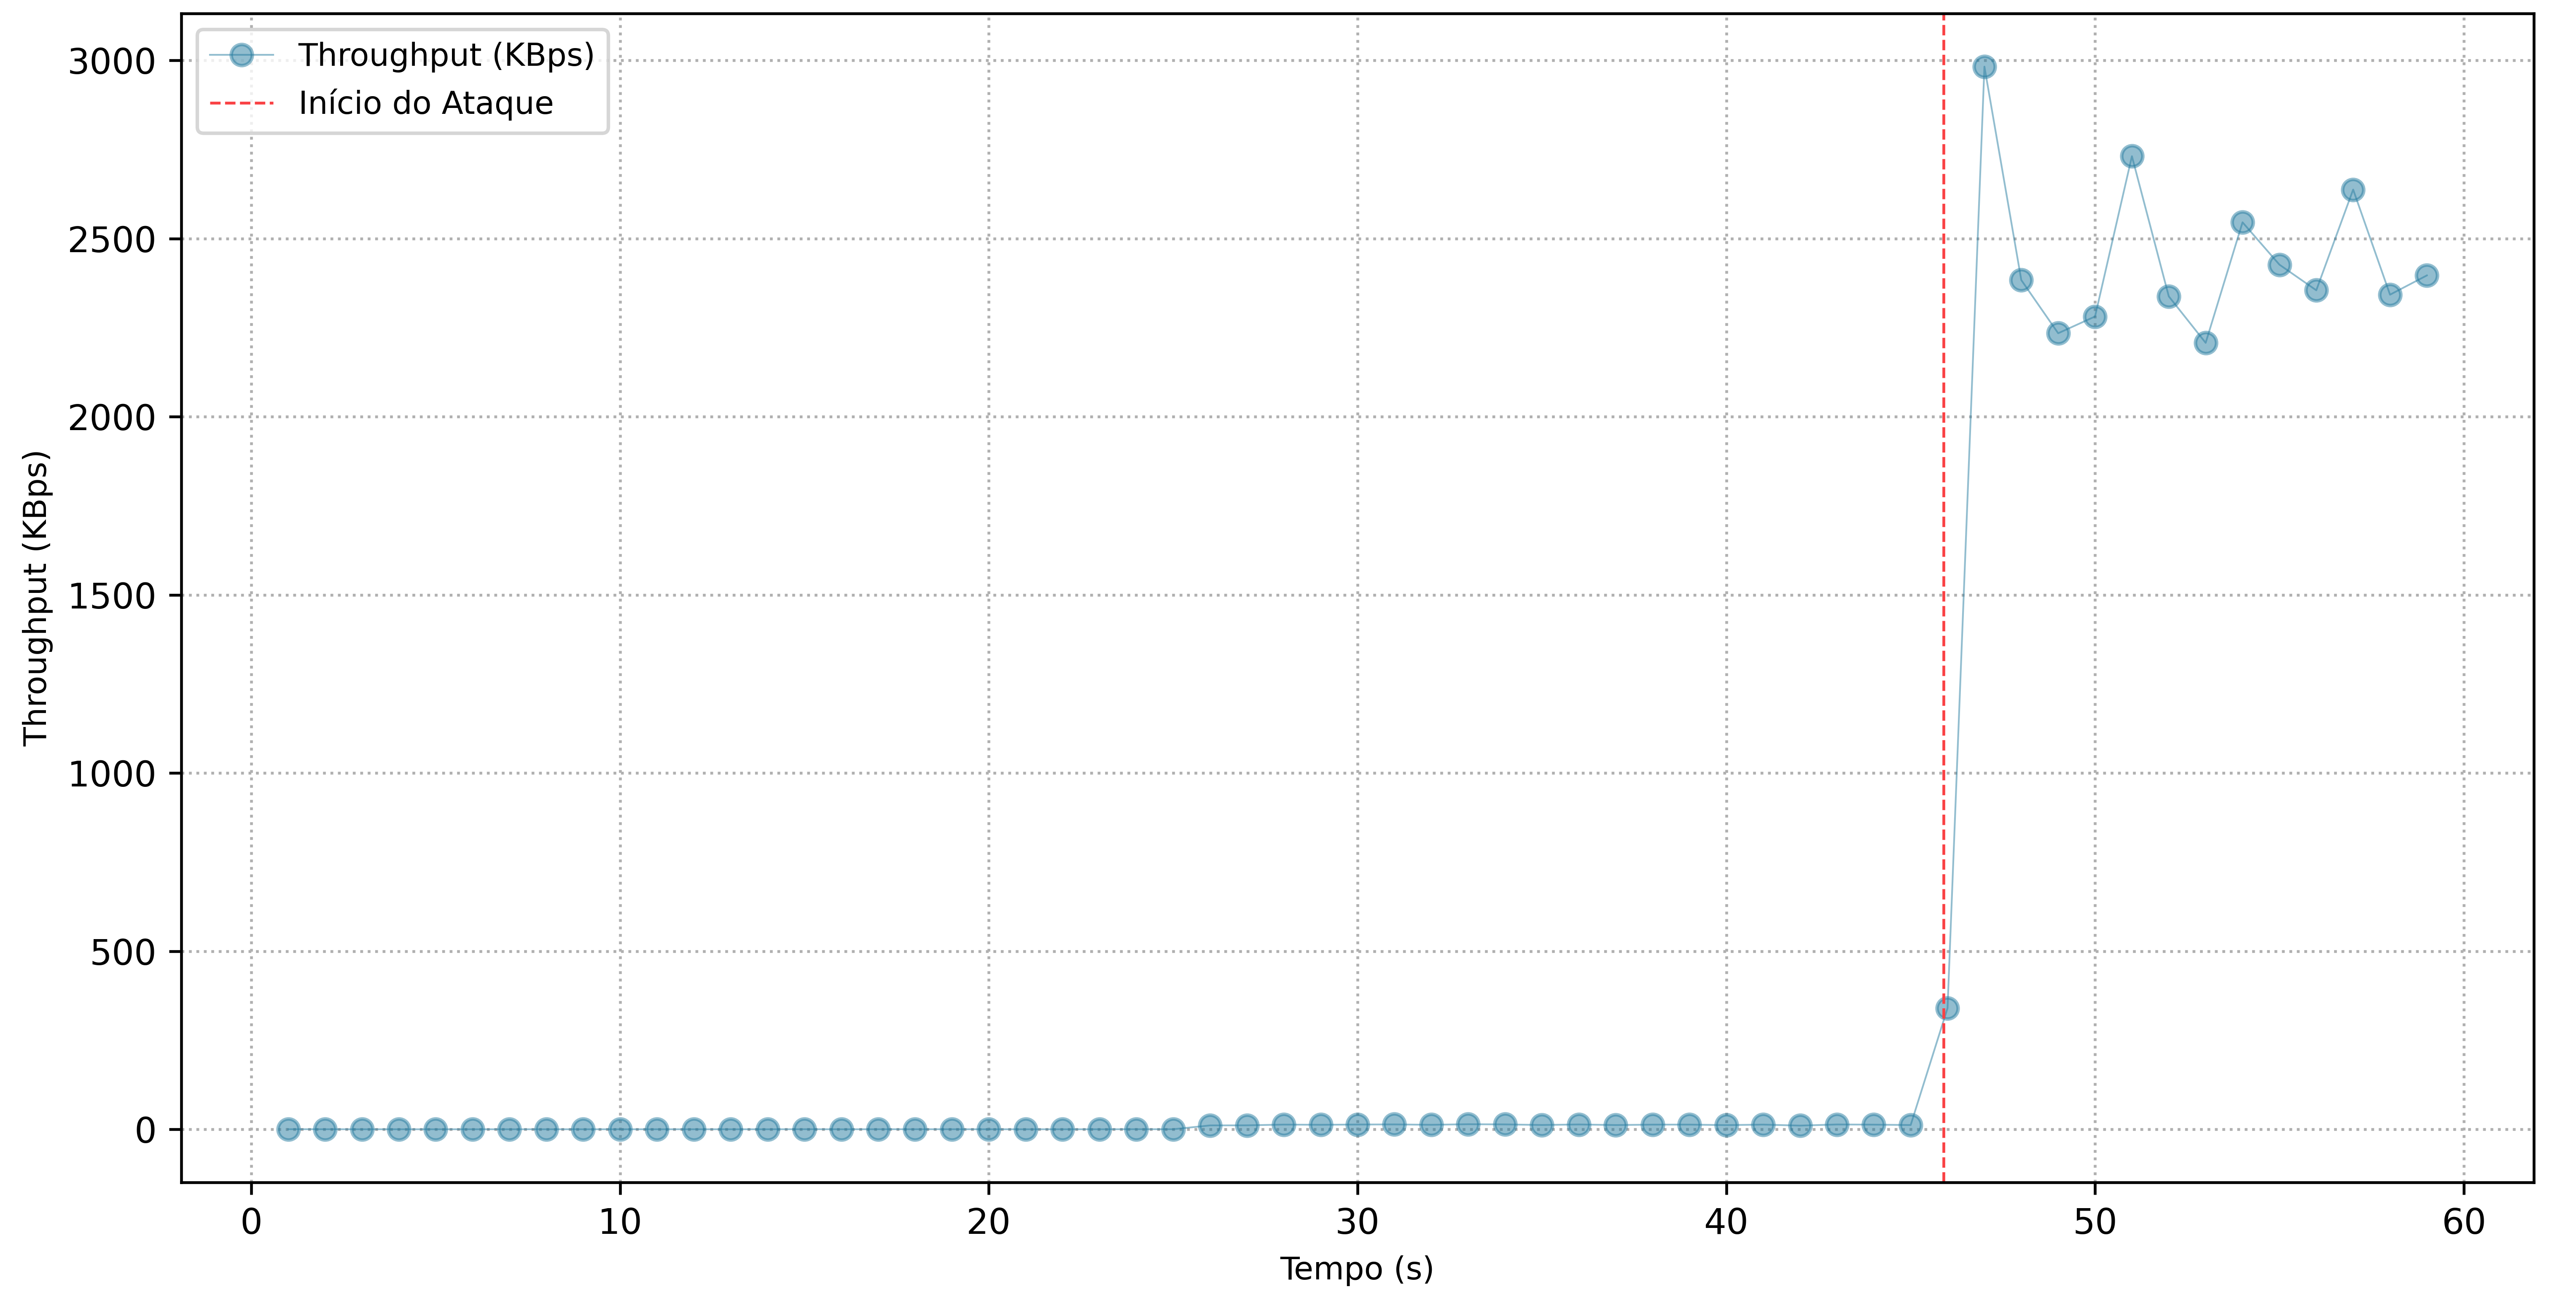
\includegraphics[width=1\textwidth, height=120pt]{USPSC-img/output/cropped/1-dos_hping3-tput.png}
        \caption{\textit{Throughput}}
    \end{subfigure}%
    ~ 
    \begin{subfigure}[t]{0.5\textwidth}
        \centering
        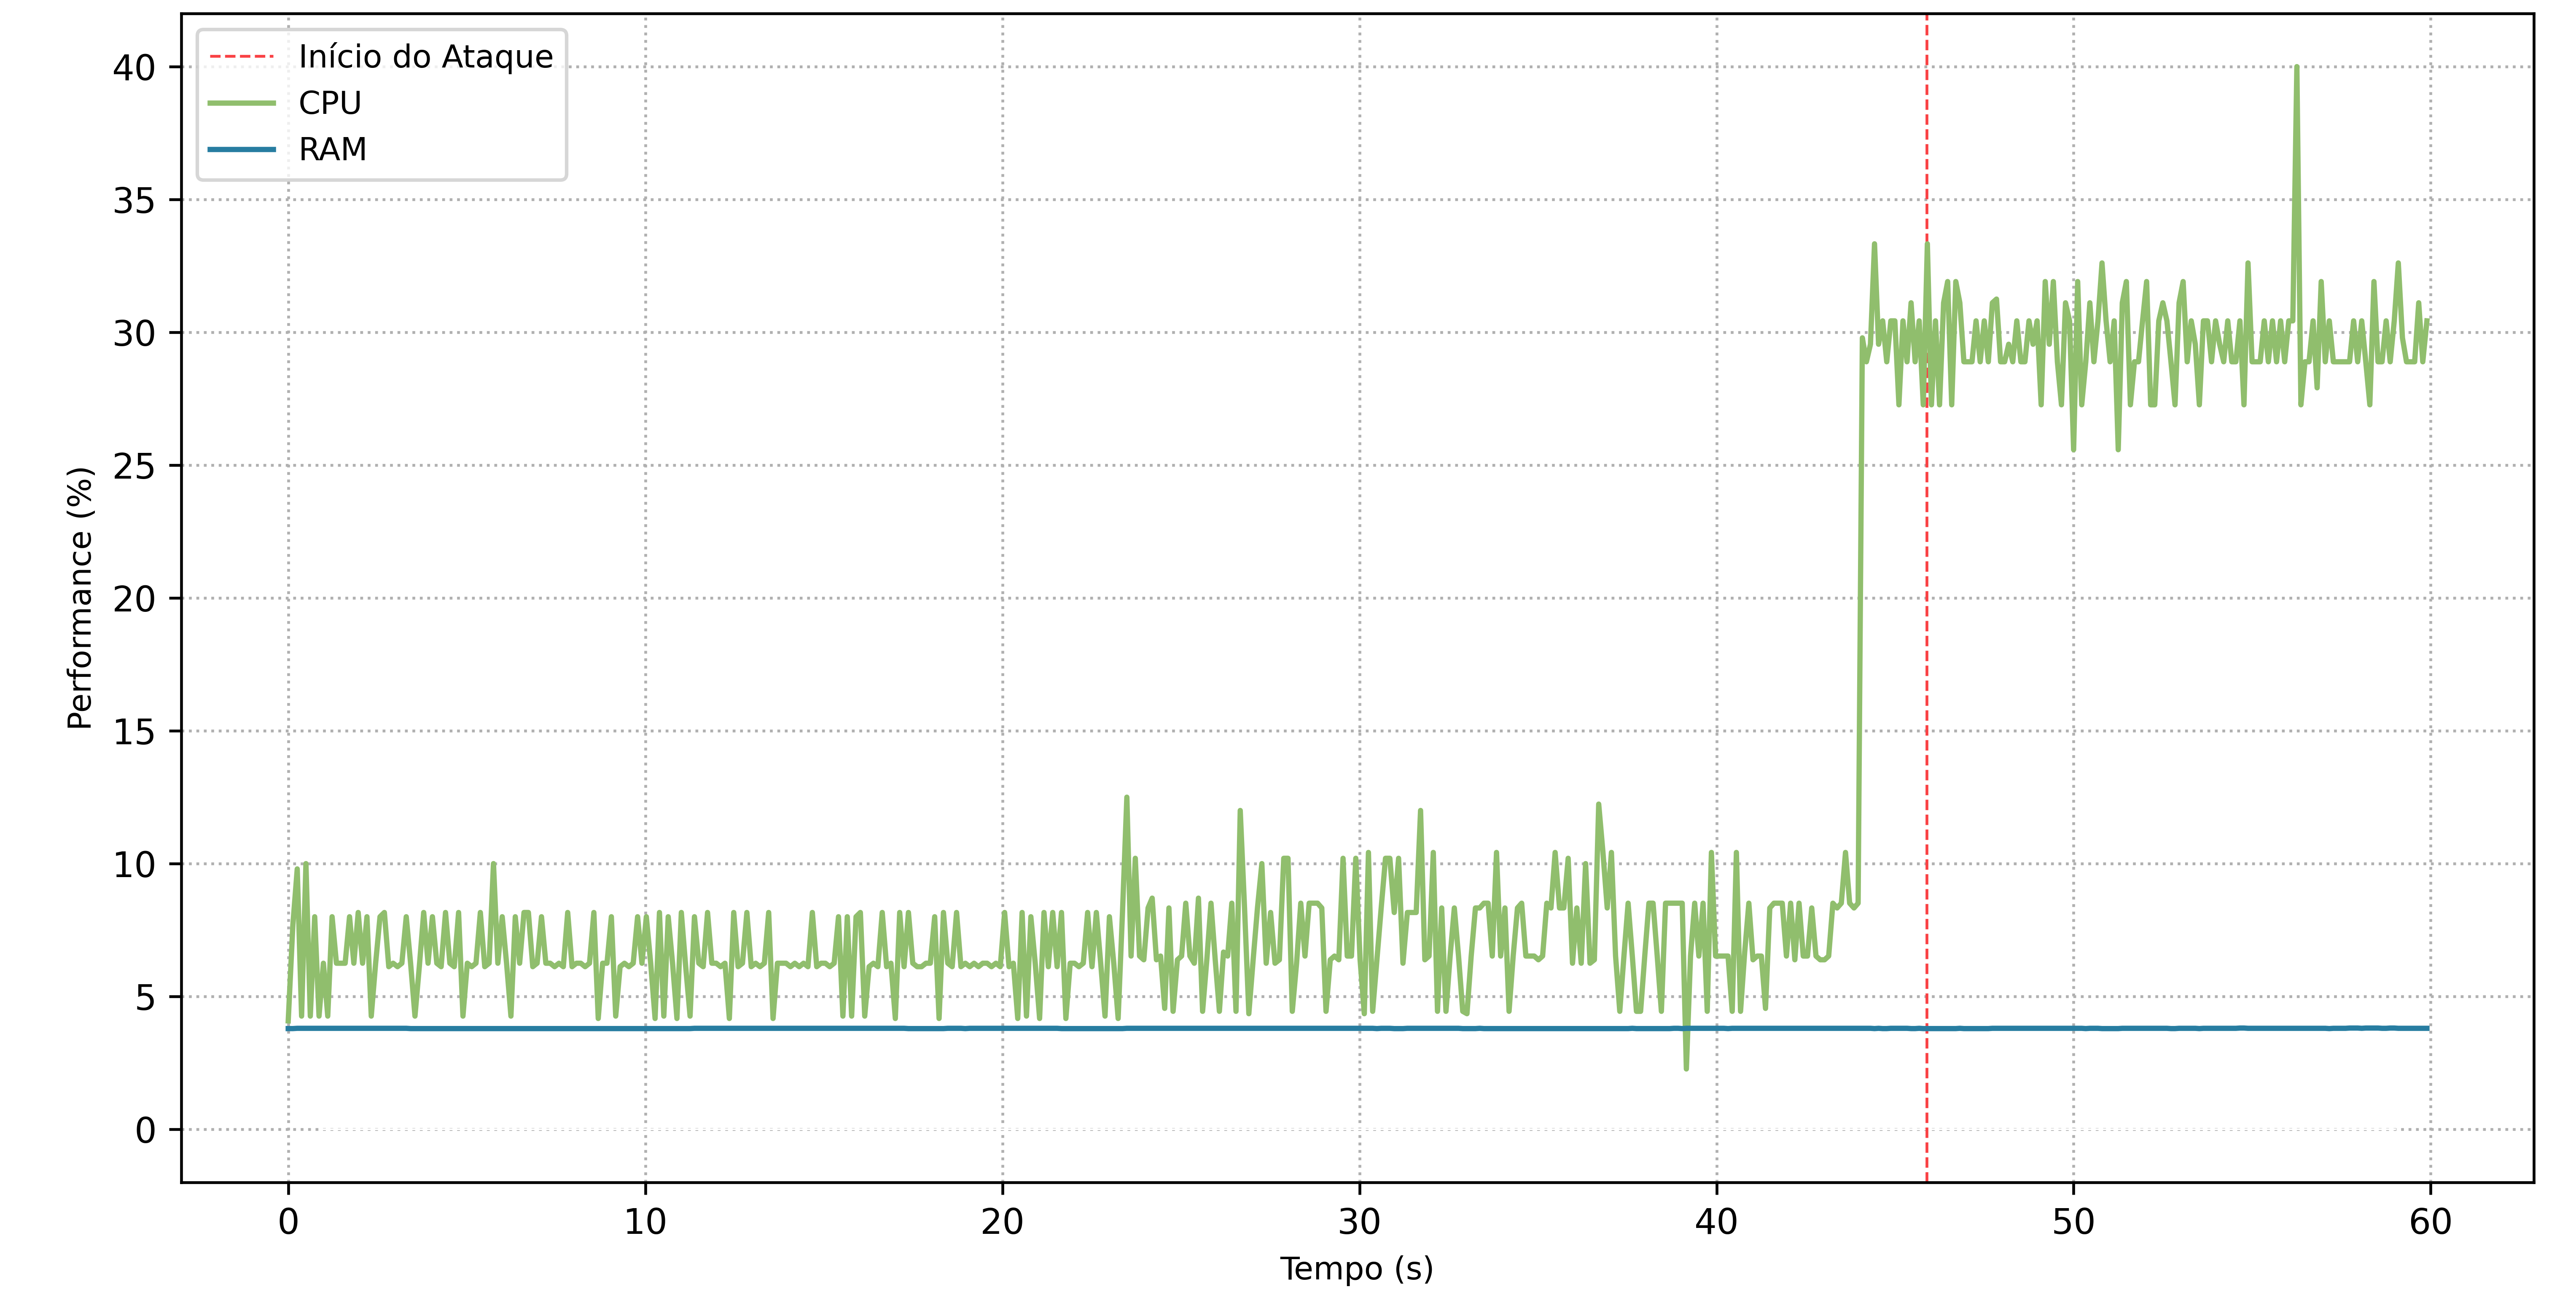
\includegraphics[width=1\textwidth, height=120pt]{USPSC-img/output/cropped/1-dos_hping3-perf.png}
        \caption{Desempenho}
    \end{subfigure}%
    \\
    \begin{subfigure}[t]{0.5\textwidth}
        \centering
        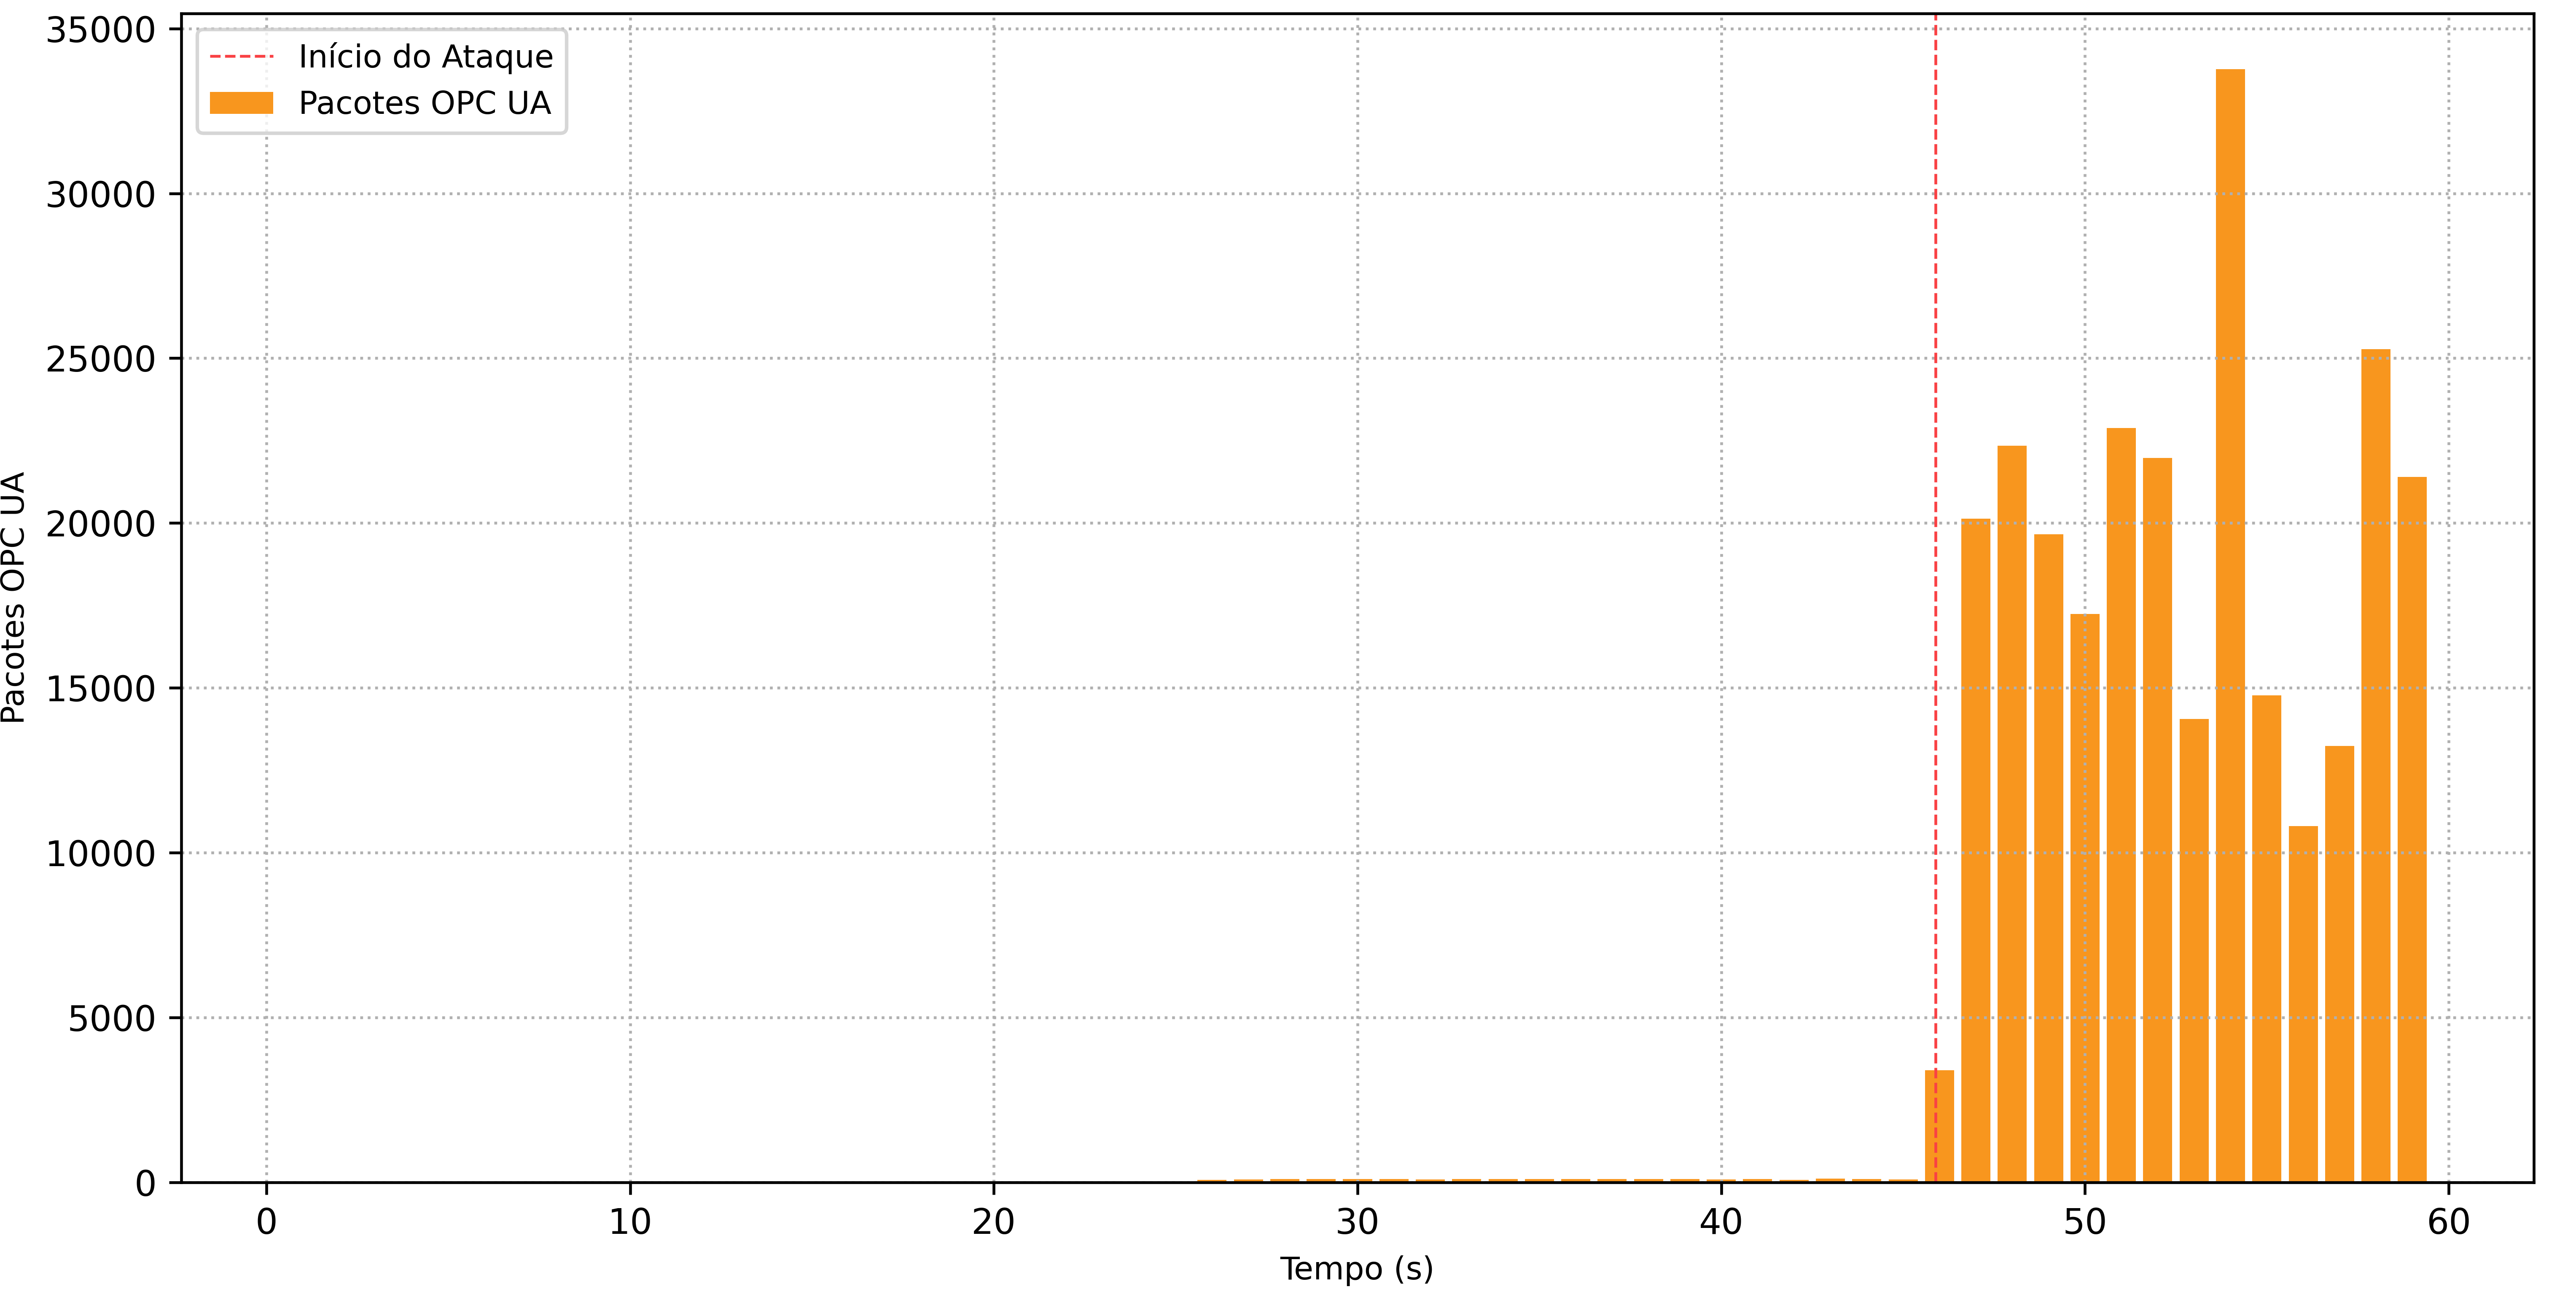
\includegraphics[width=1\textwidth, height=120pt]{USPSC-img/output/cropped/1-dos_hping3-pack.png}
        \caption{Pacotes OPC UA}
    \end{subfigure}%
    ~
    \begin{subfigure}[t]{0.5\textwidth}
        \centering
        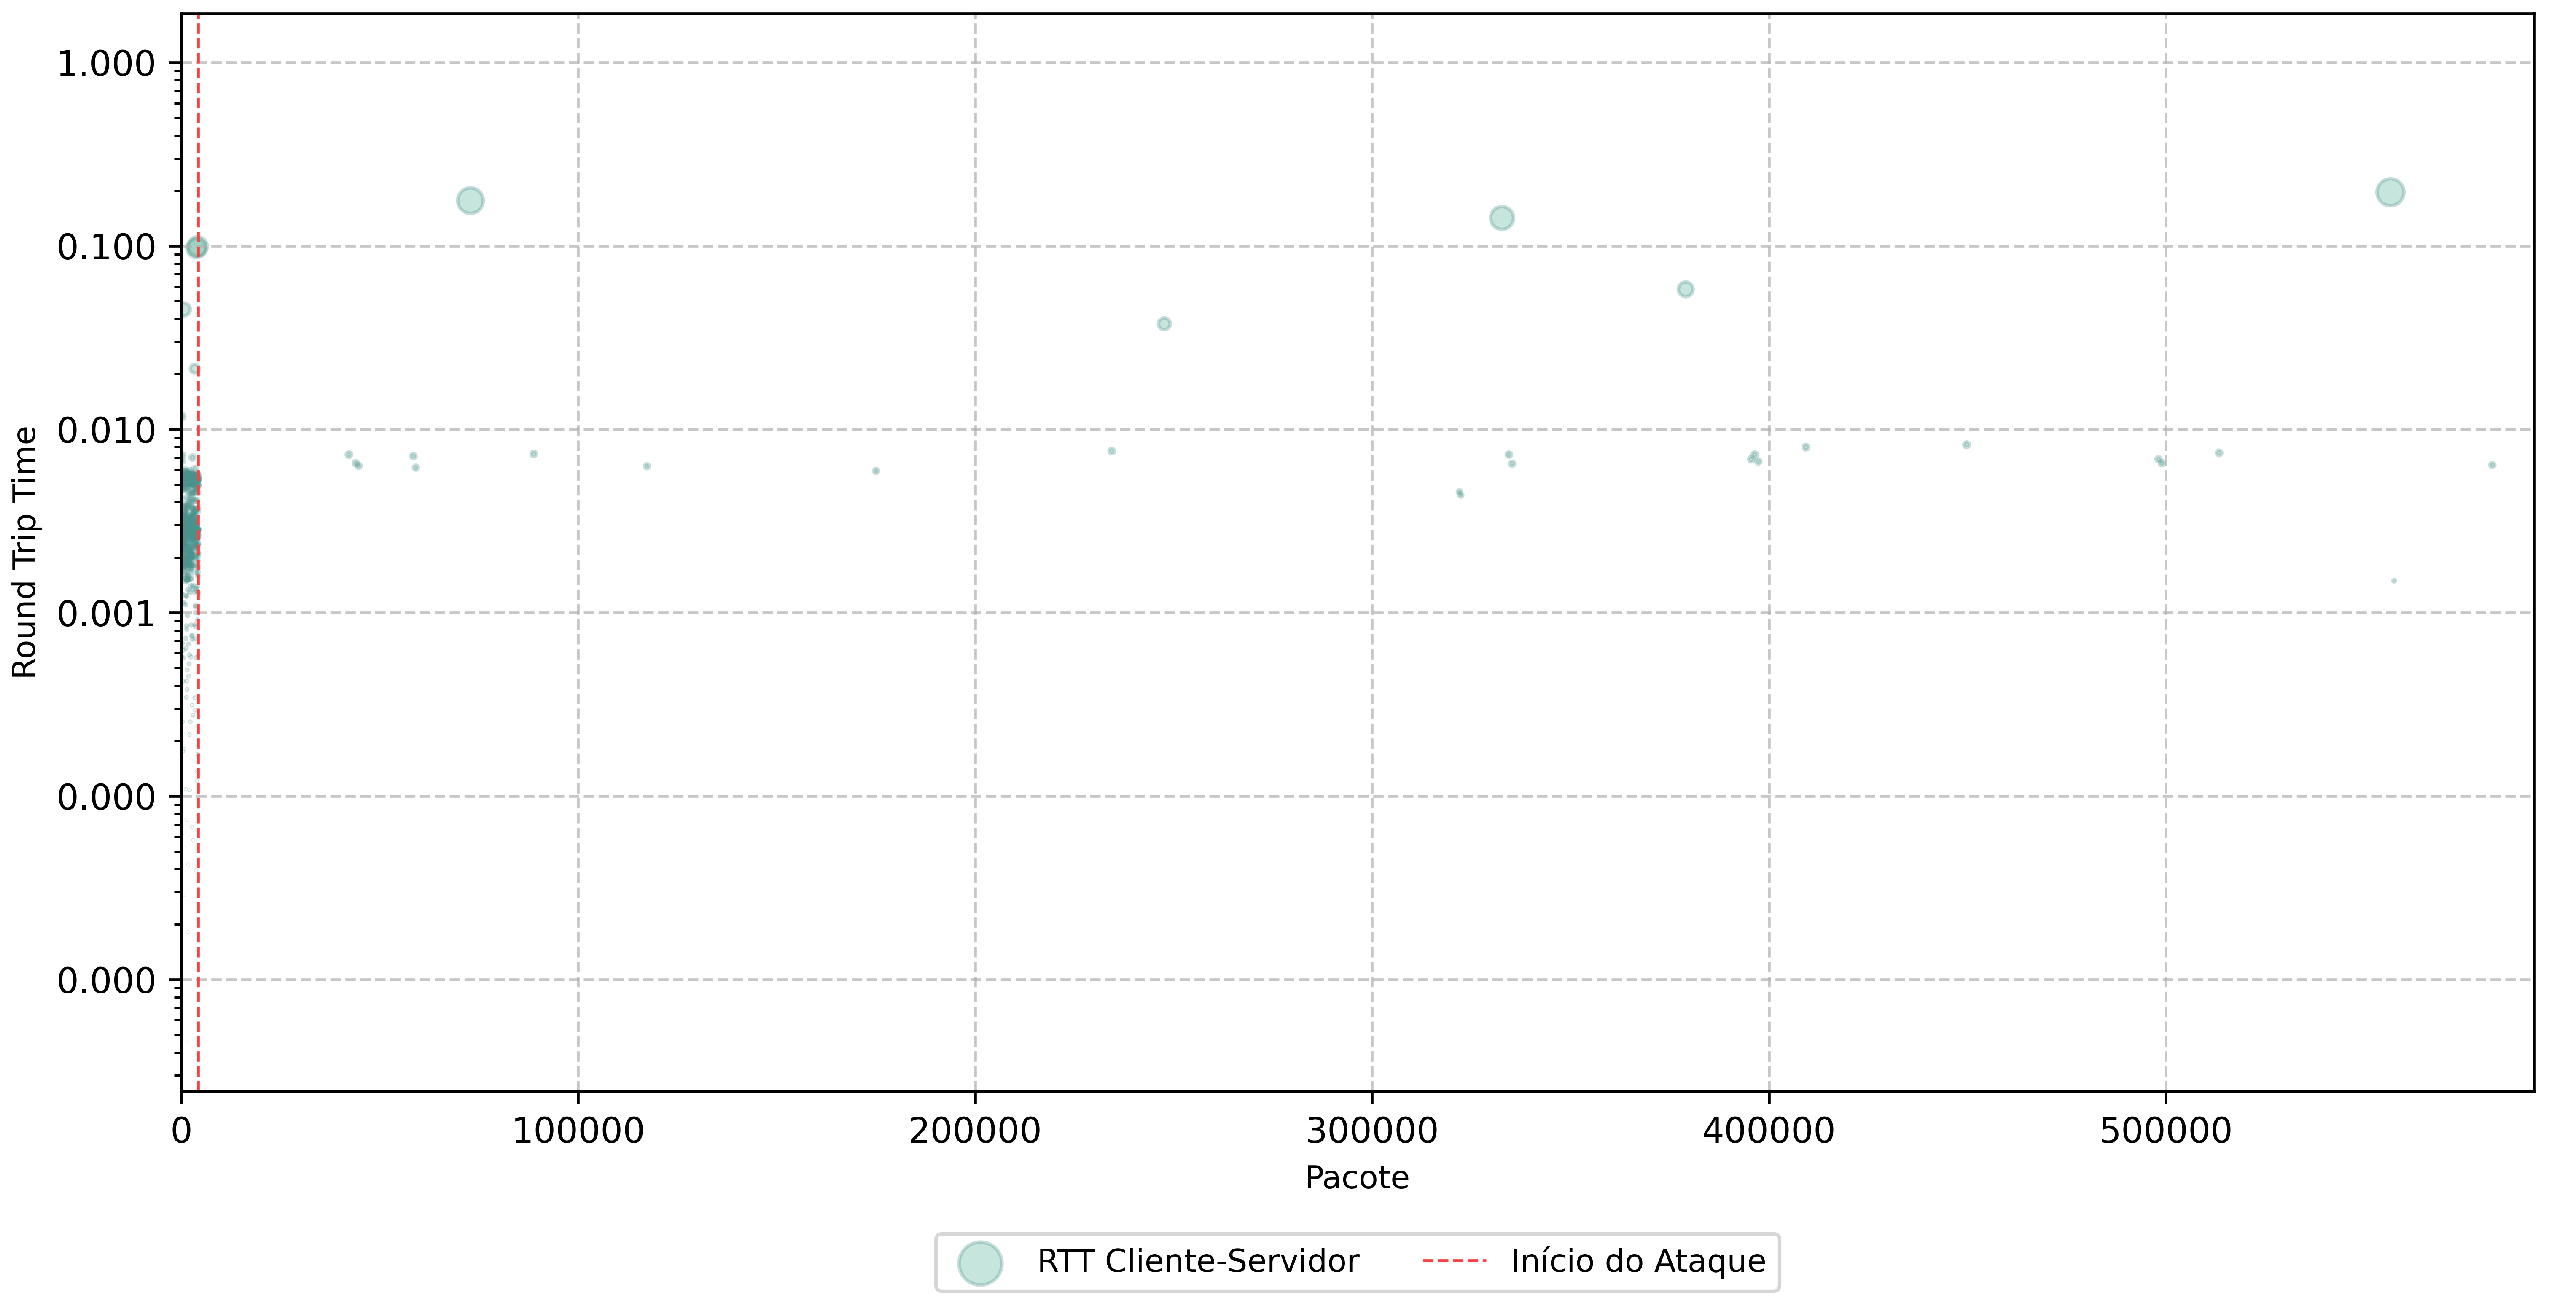
\includegraphics[width=1\textwidth, height=120pt]{USPSC-img/output/cropped/1-dos_hping3-rttp.png}
        \caption{RTT por pacote}
    \end{subfigure}%
    % ~
    % \begin{subfigure}[t]{0.5\textwidth}
    %     \centering
    %     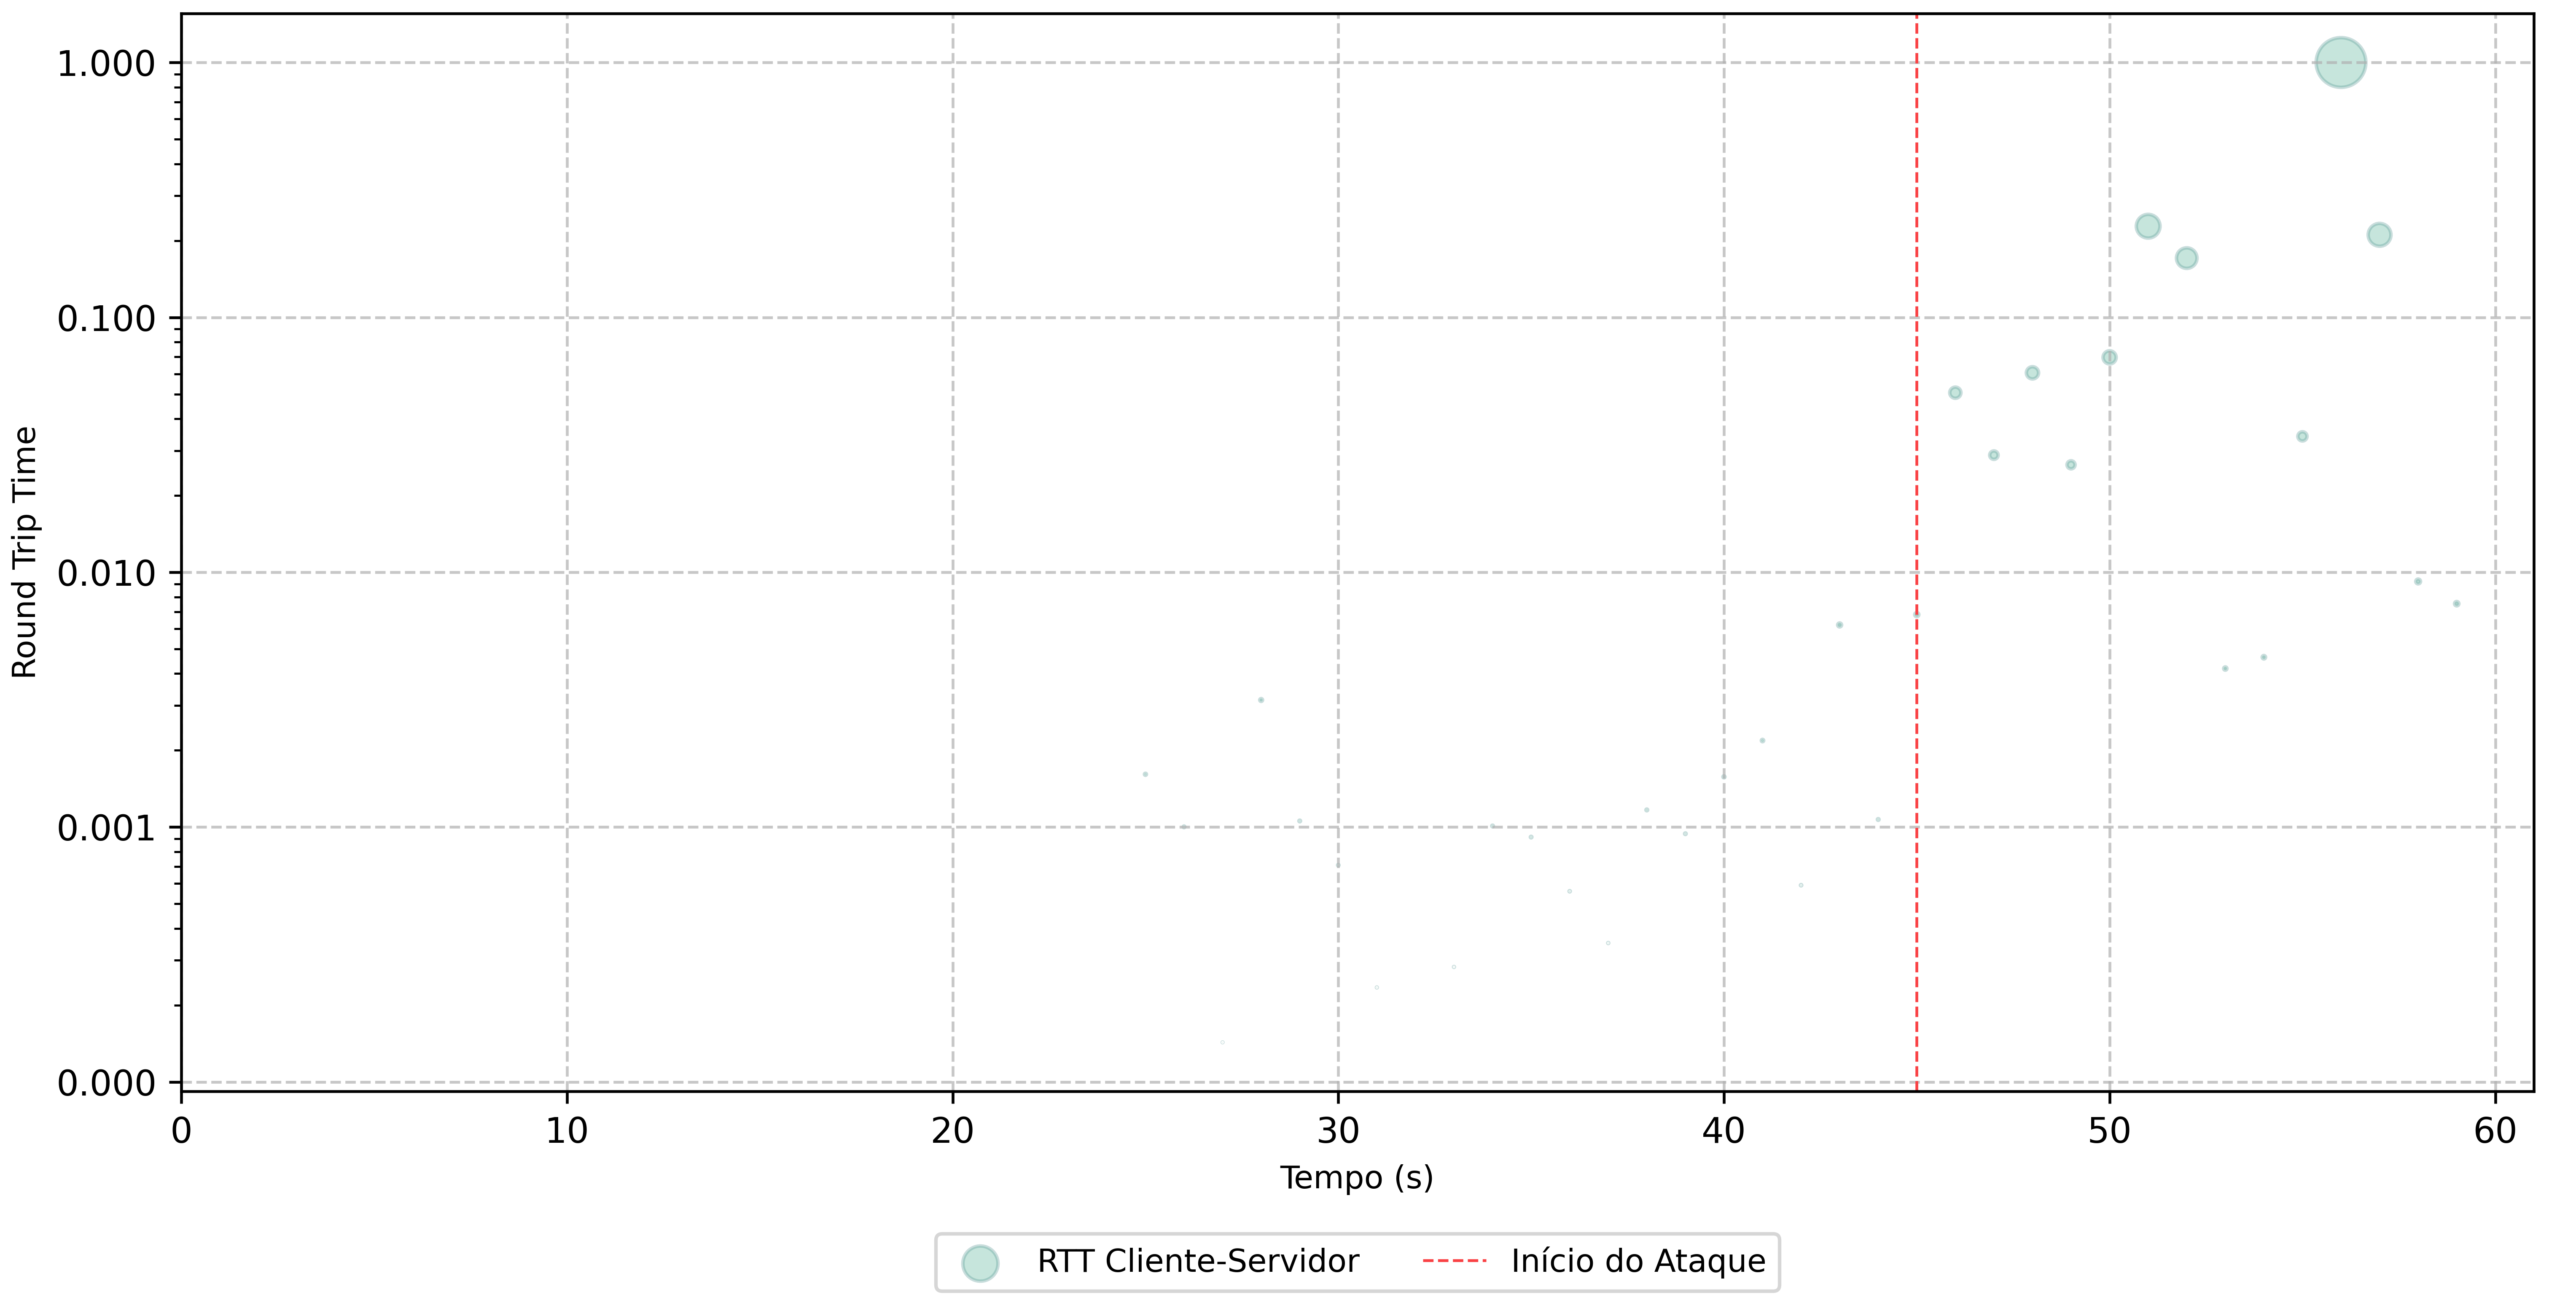
\includegraphics[width=1\textwidth, height=120pt]{USPSC-img/output/cropped/1-dos_hping3-rtts.png}
    %     \caption{RTT por segundos}
    % \end{subfigure}%
    \label{fig:1-dos_hping3}
    \caption{Gráficos do ataque de DoS por inundação TCP/IP - nível de segurança: `Sign'.}
\end{figure}

\begin{figure}[htbp!]
    \centering
    \begin{subfigure}[t]{0.5\textwidth}
        \centering
        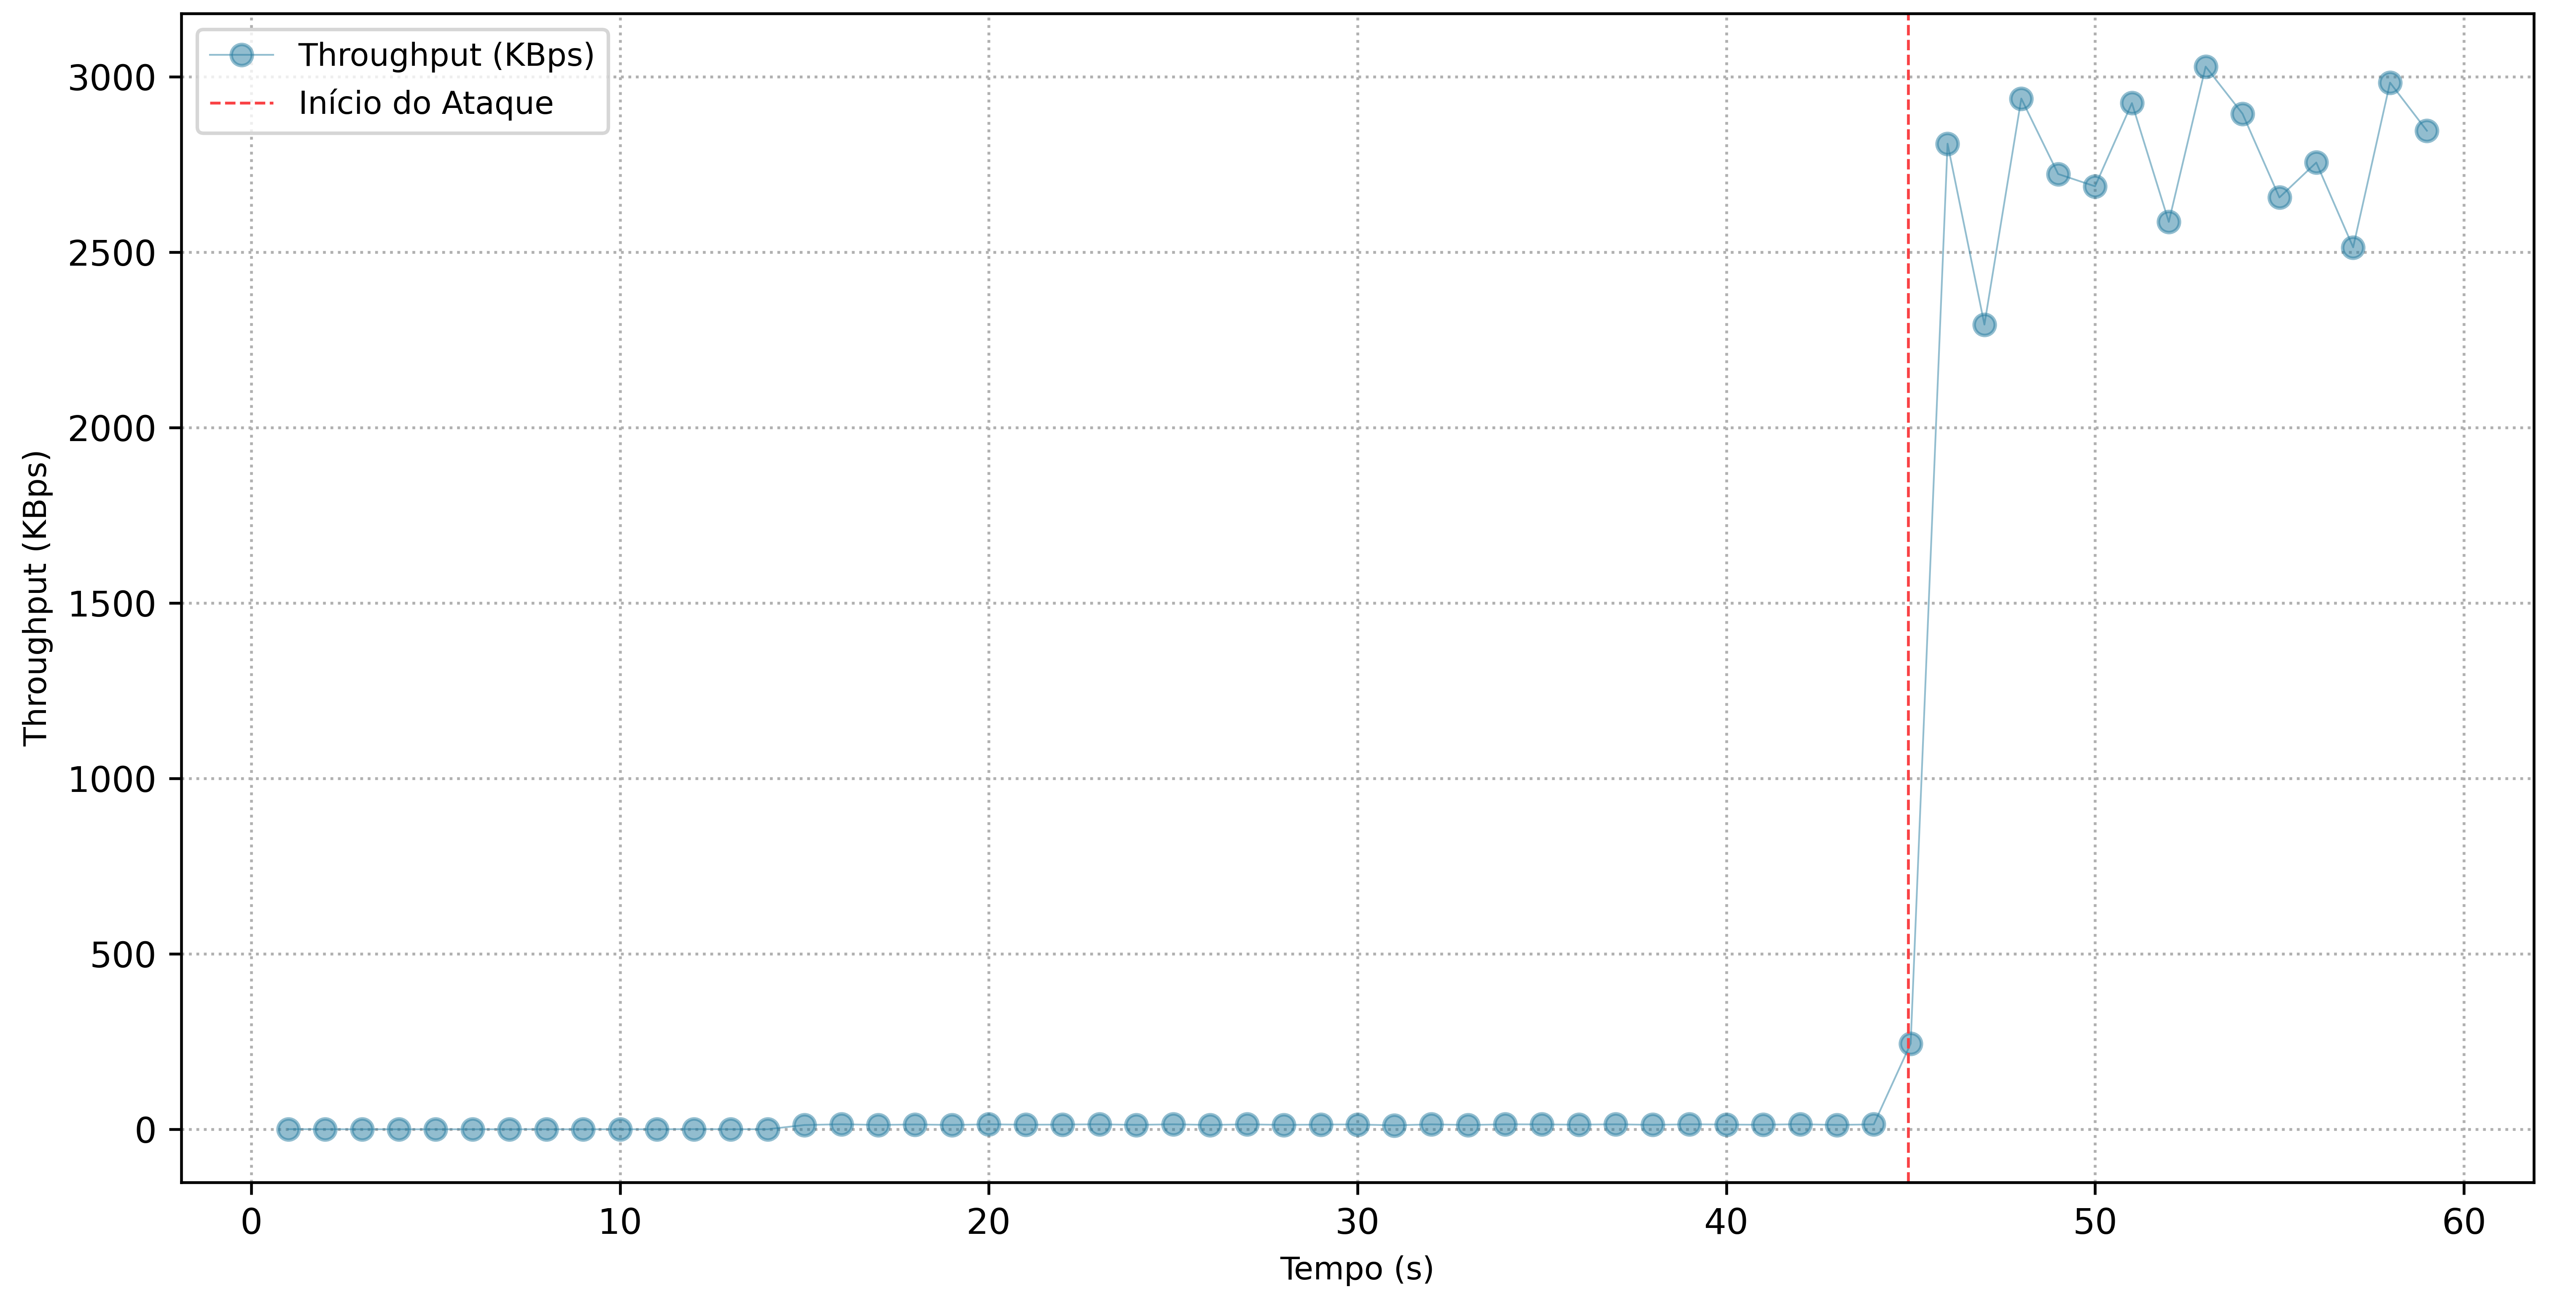
\includegraphics[width=1\textwidth, height=120pt]{USPSC-img/output/cropped/2-dos_hping3-tput.png}
        \caption{\textit{Throughput}}
    \end{subfigure}%
    ~ 
    \begin{subfigure}[t]{0.5\textwidth}
        \centering
        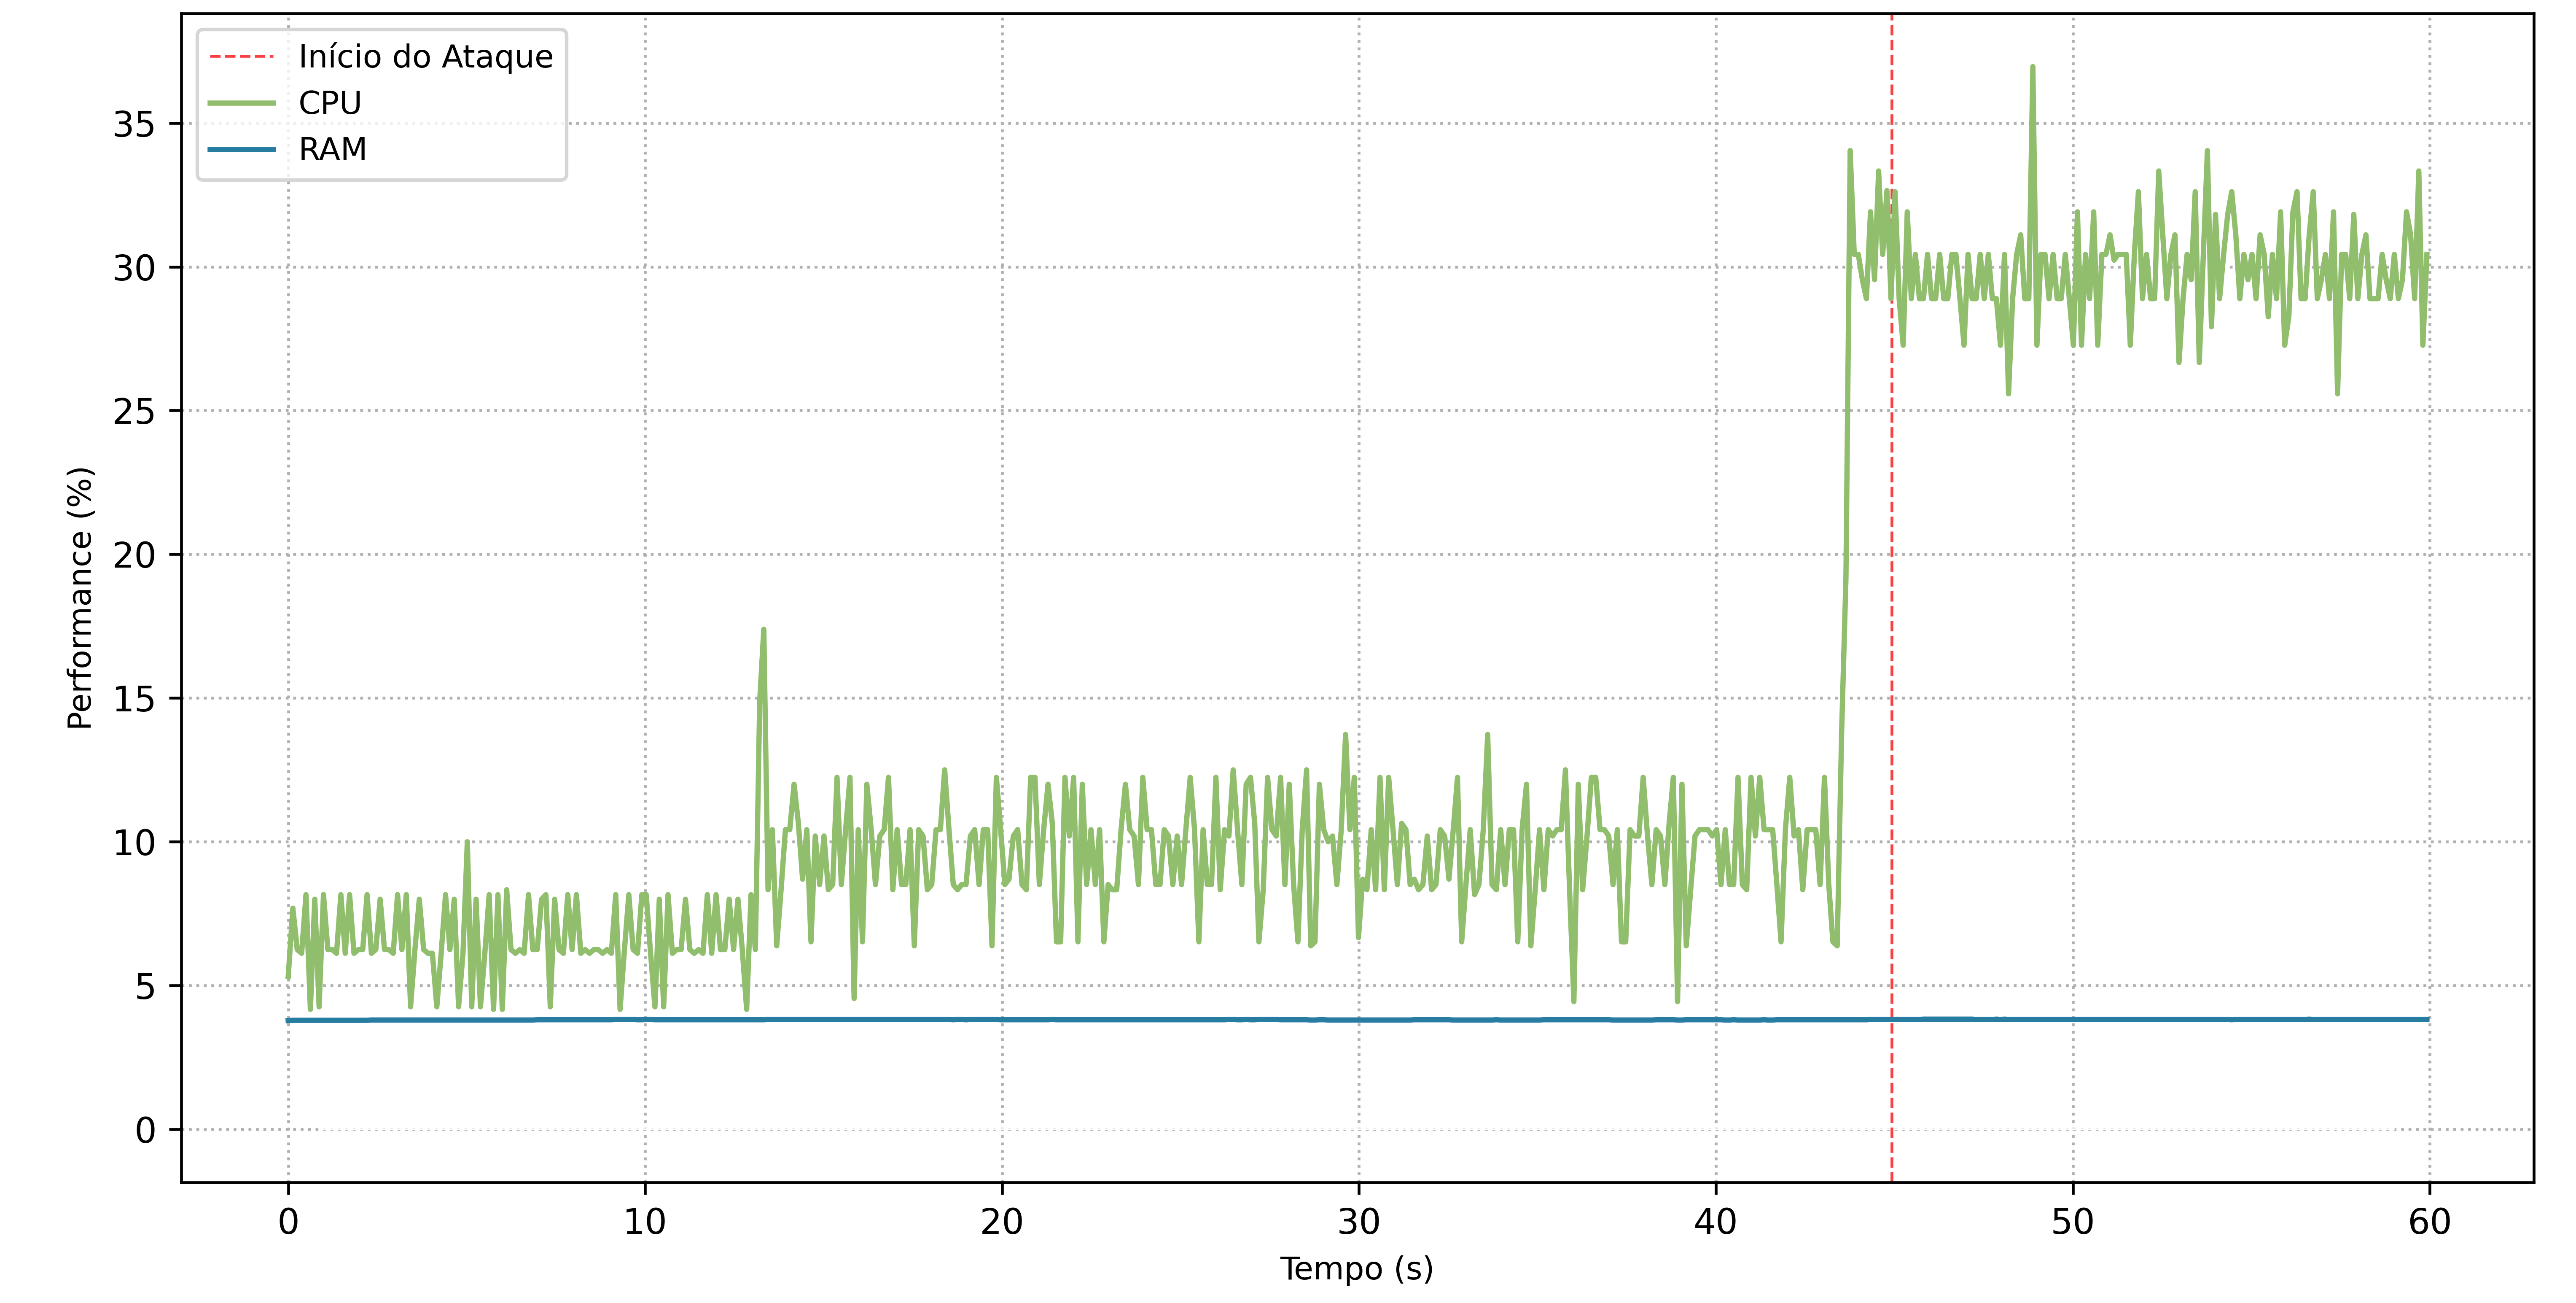
\includegraphics[width=1\textwidth, height=120pt]{USPSC-img/output/cropped/2-dos_hping3-perf.png}
        \caption{Desempenho}
    \end{subfigure}%
    \\
    % \begin{subfigure}[t]{0.5\textwidth}
    %     \centering
    %     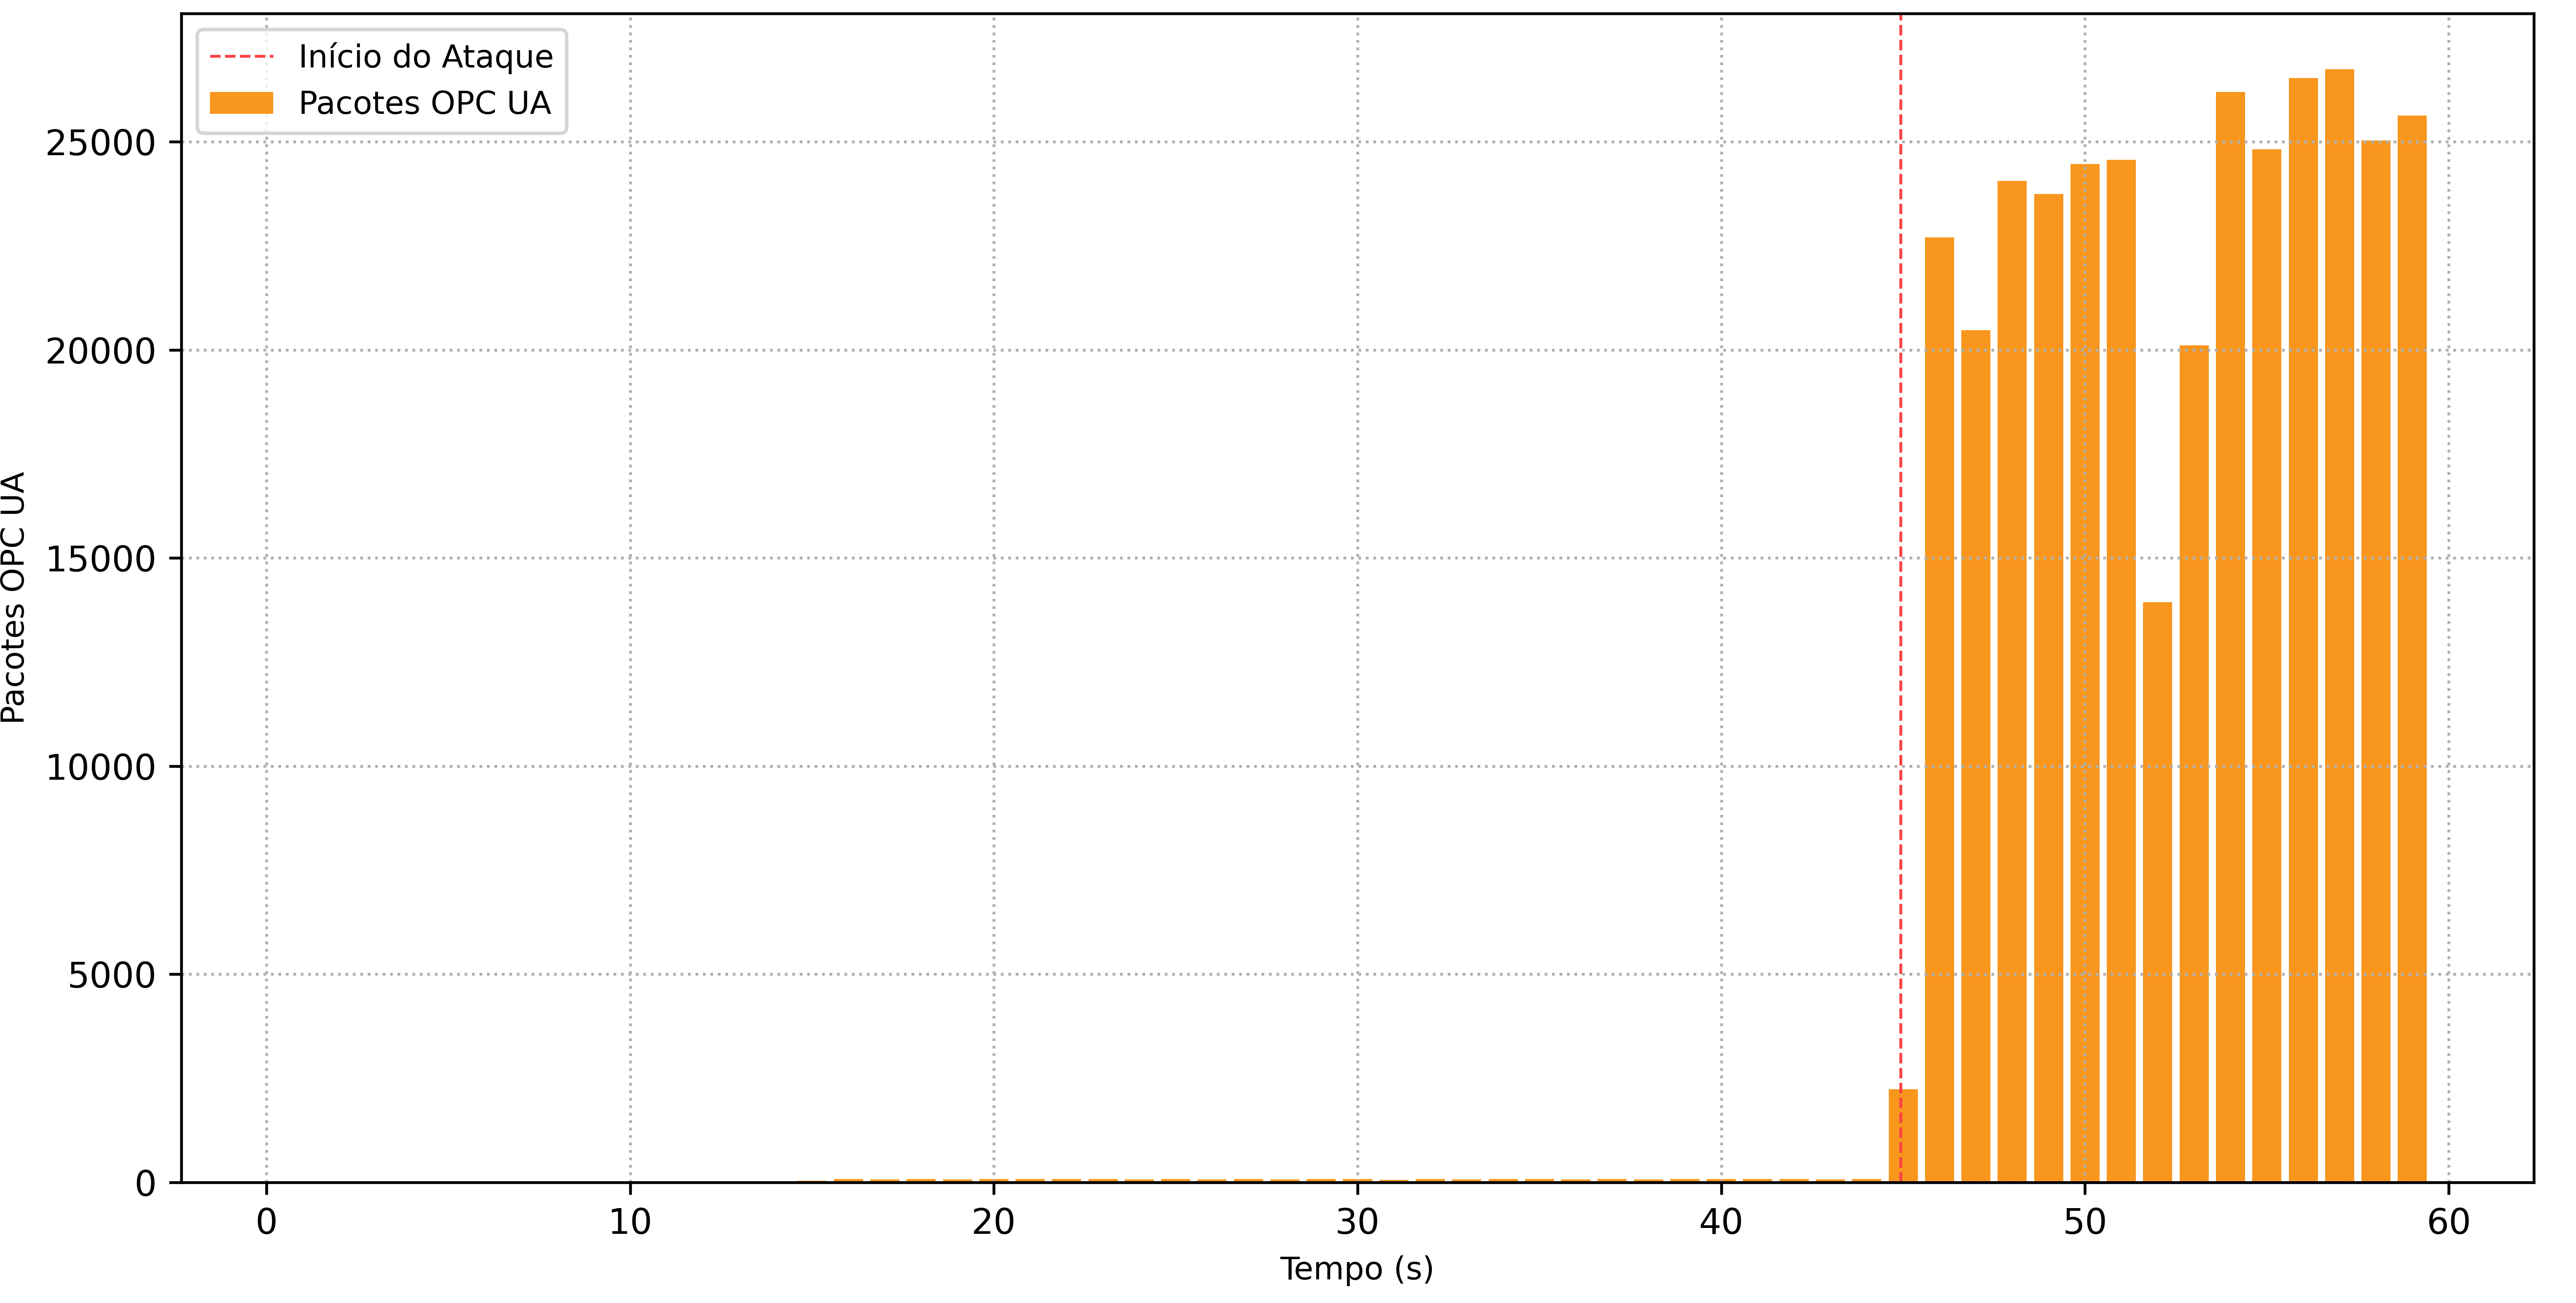
\includegraphics[width=1\textwidth, height=120pt]{USPSC-img/output/cropped/2-dos_hping3-pack.png}
    %     \caption{Pacotes OPC UA}
    % \end{subfigure}%
    % ~
    \begin{subfigure}[t]{0.5\textwidth}
        \centering
        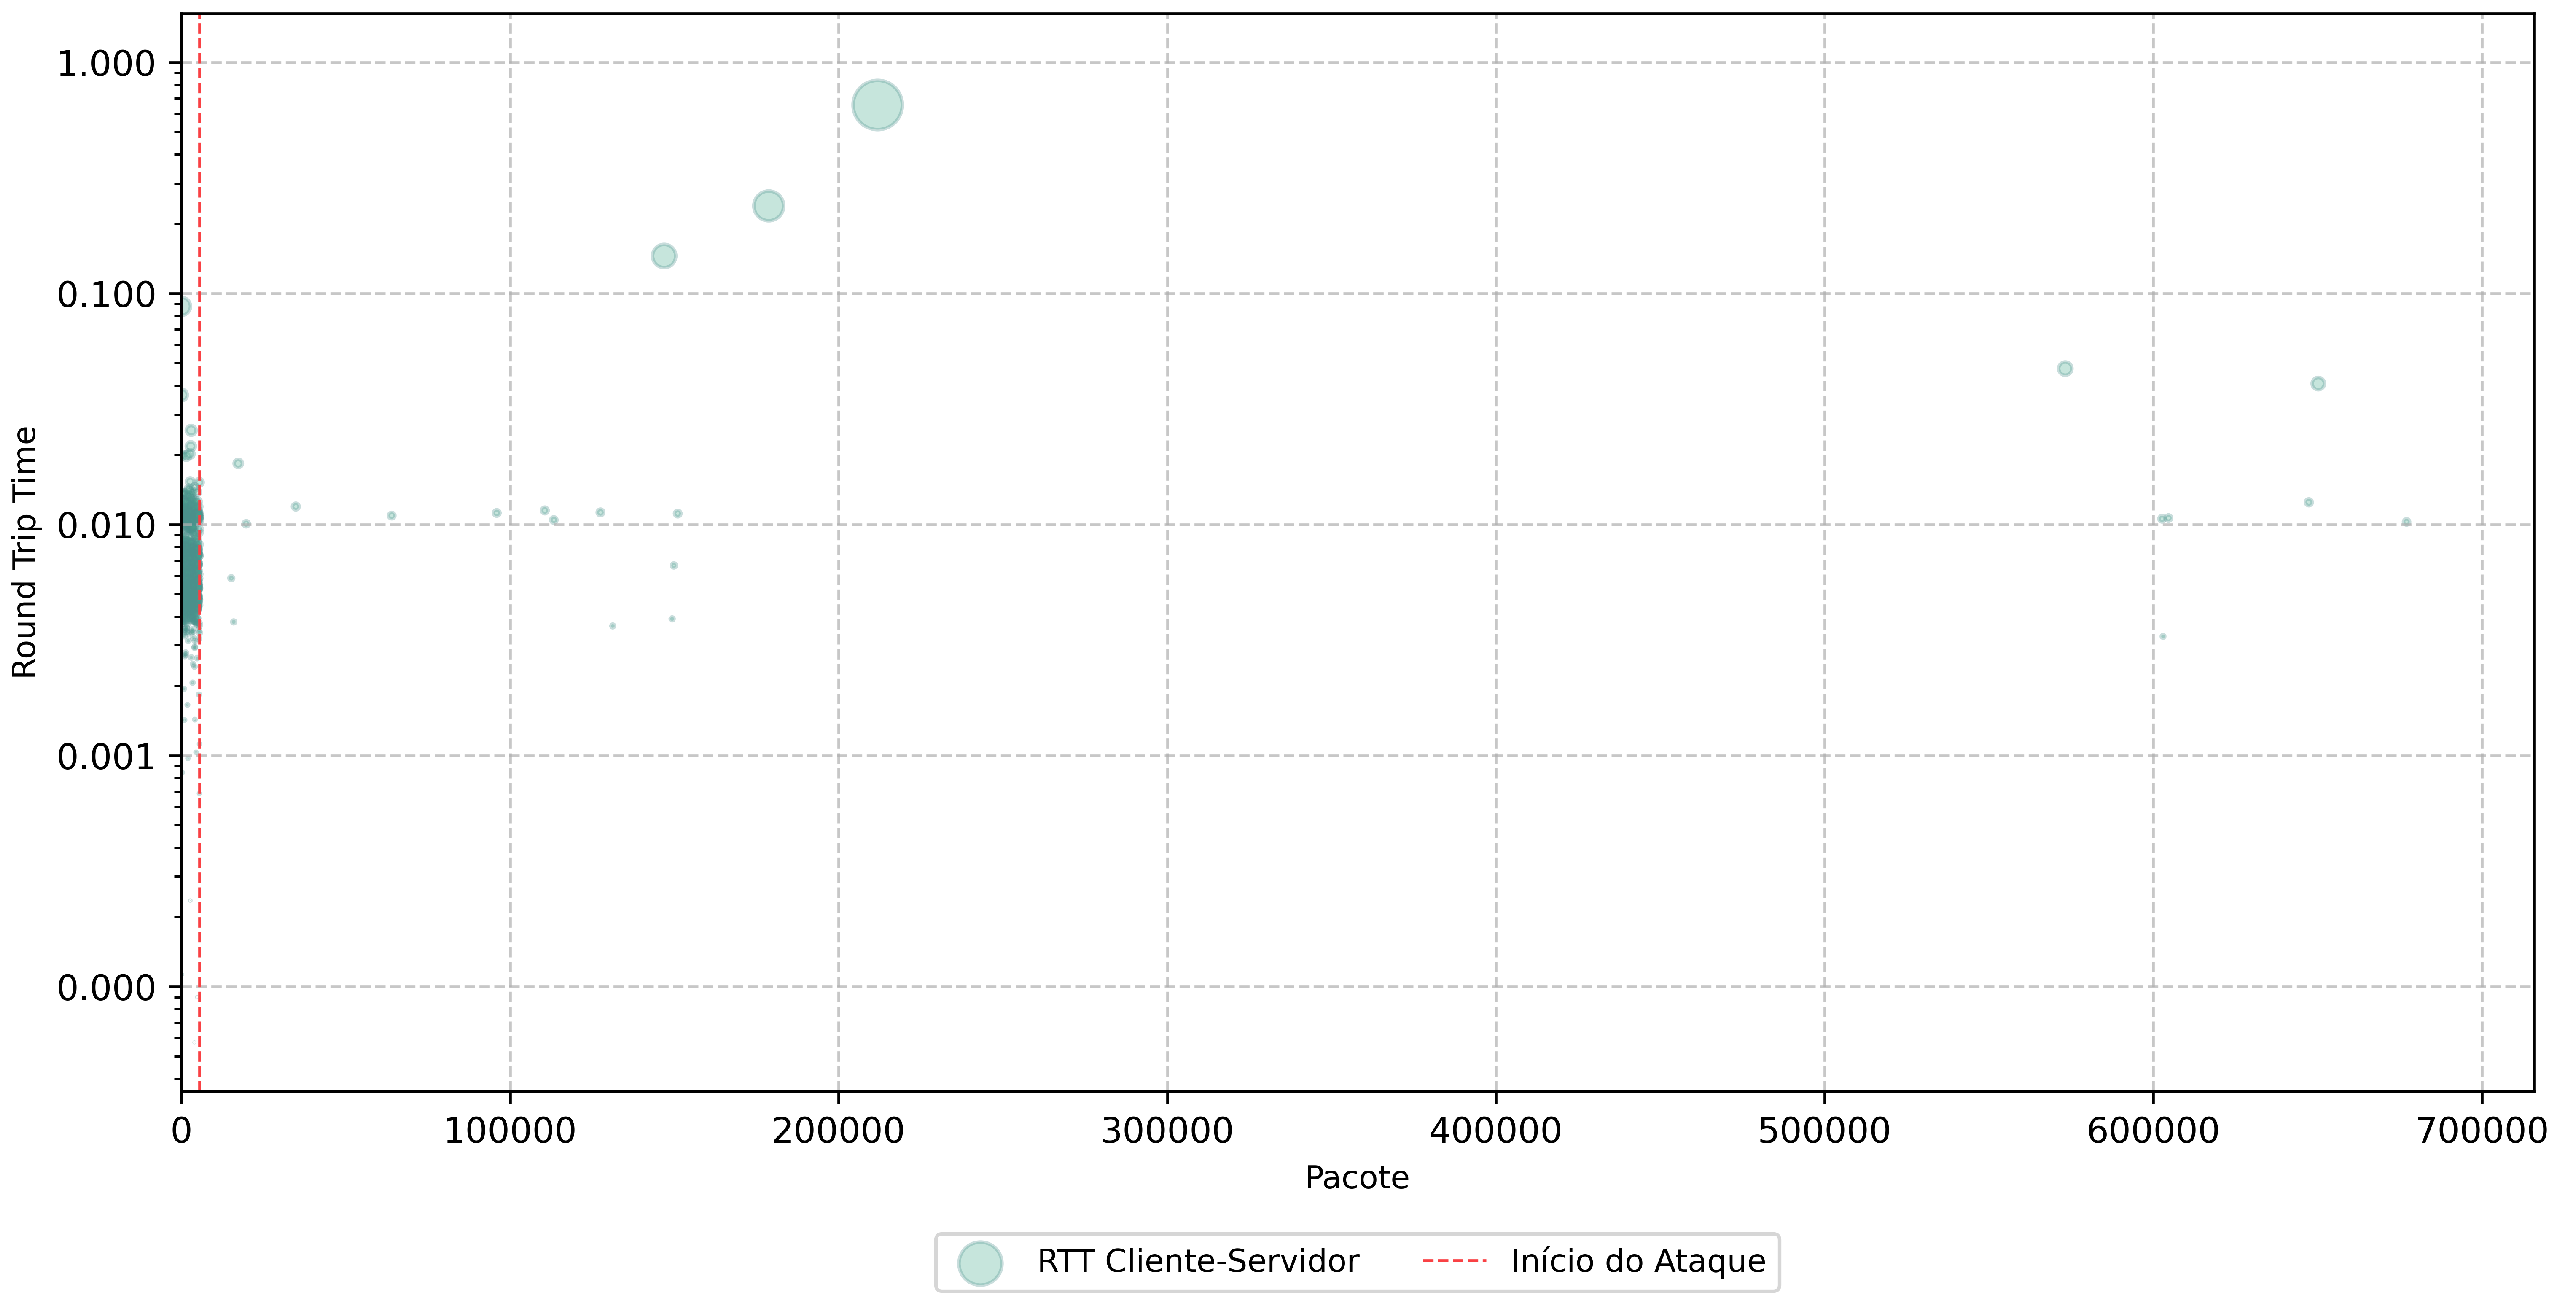
\includegraphics[width=1\textwidth, height=120pt]{USPSC-img/output/cropped/2-dos_hping3-rttp.png}
        \caption{RTT por pacote}
    \end{subfigure}%
    ~
    \begin{subfigure}[t]{0.5\textwidth}
        \centering
        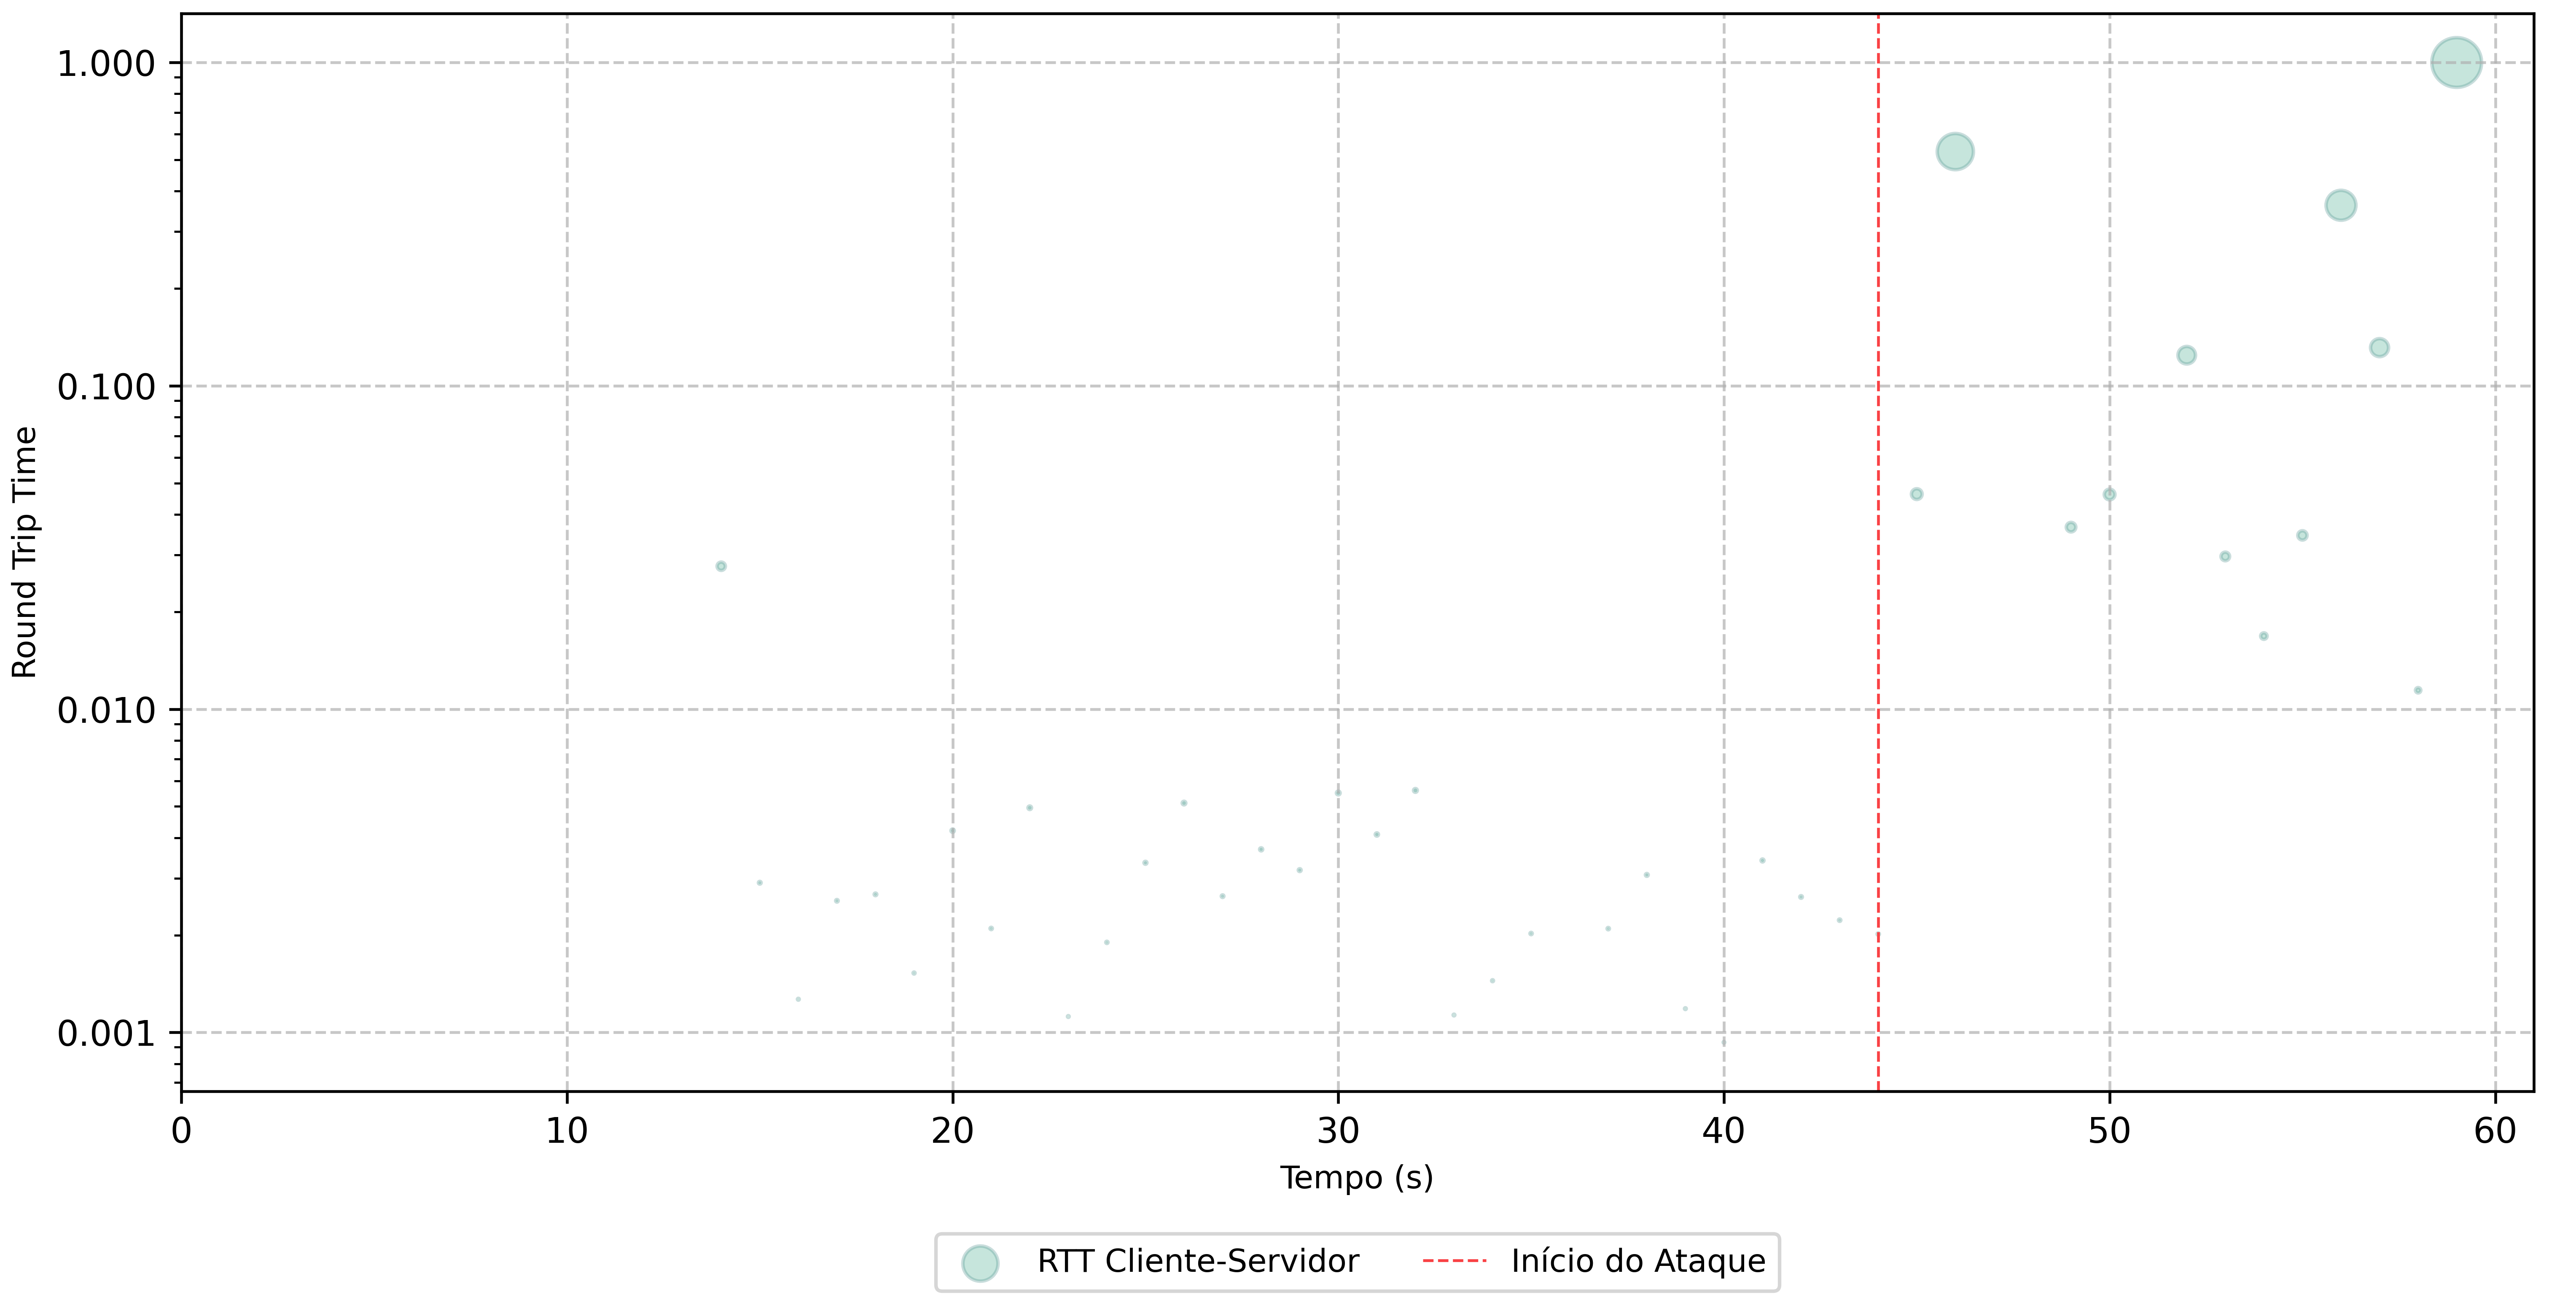
\includegraphics[width=1\textwidth, height=120pt]{USPSC-img/output/cropped/2-dos_hping3-rtts.png}
        \caption{RTT por segundos}
    \end{subfigure}%
    \label{fig:2-dos_hping3}
    \caption{Gráficos do ataque de DoS por inundação TCP/IP - nível de segurança: `Sign \& Encrypt'.}
\end{figure}

\begin{figure}[htbp!]
    \centering
    \begin{subfigure}[t]{0.5\textwidth}
        \centering
        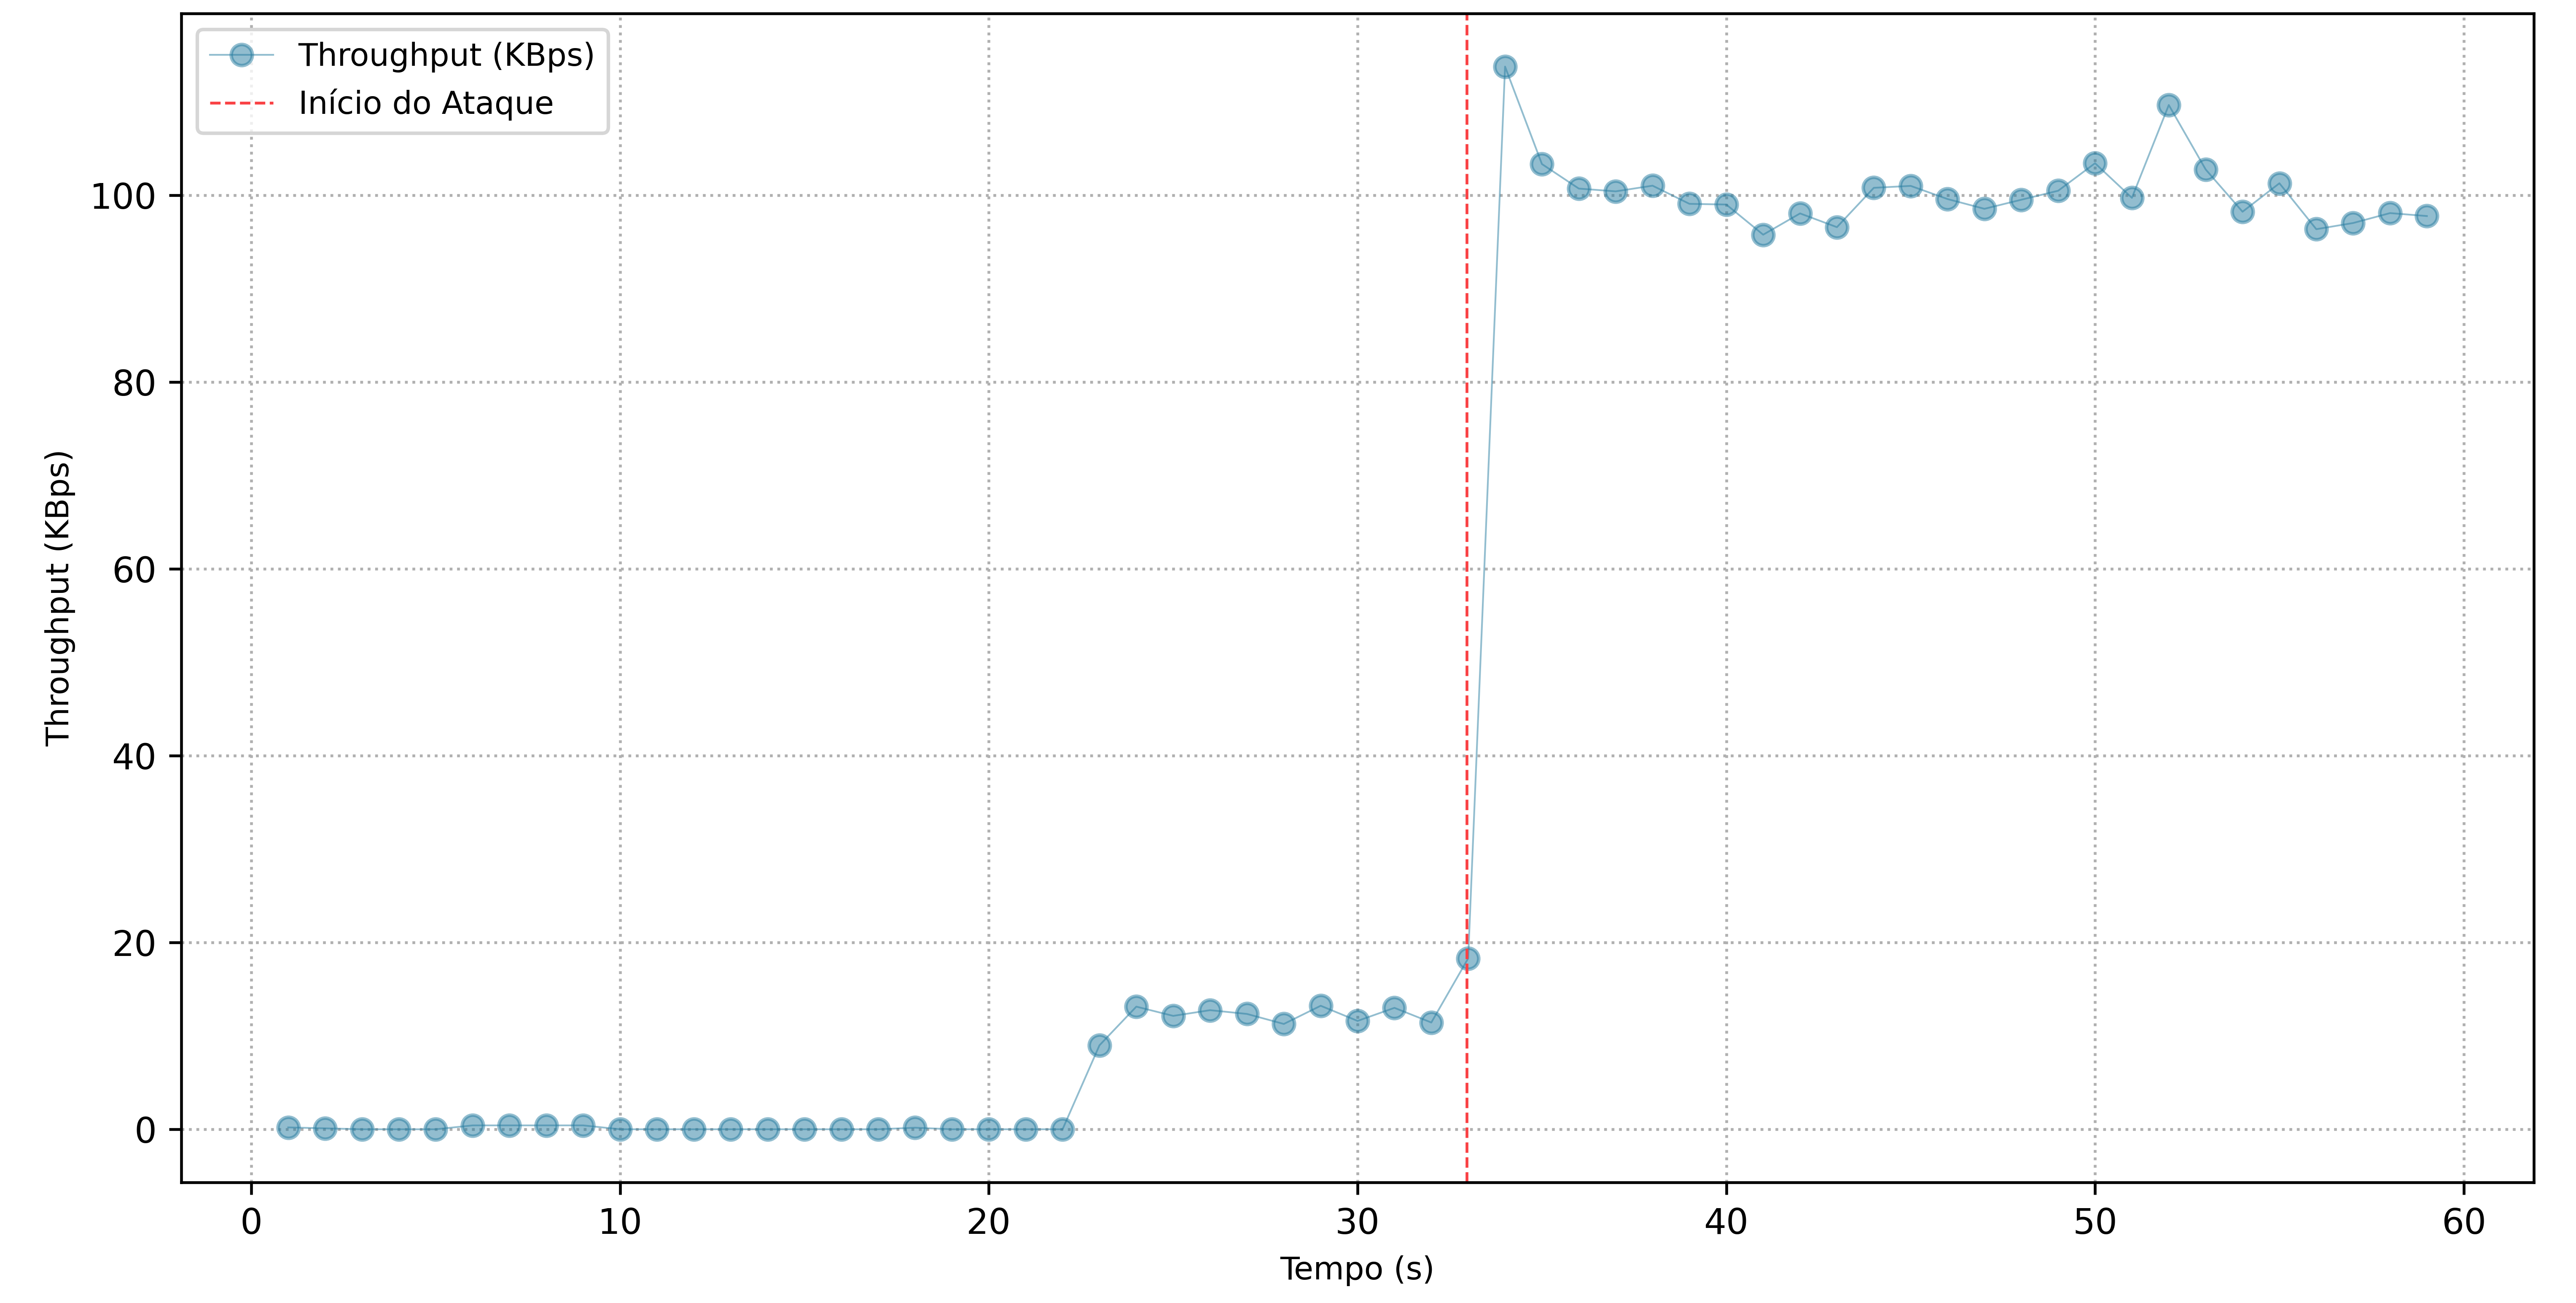
\includegraphics[width=1\textwidth, height=120pt]{USPSC-img/output/cropped/0-dos_open_multiple_secure_channels-tput.png}
        \caption{\textit{Throughput}}
    \end{subfigure}%
    ~ 
    \begin{subfigure}[t]{0.5\textwidth}
        \centering
        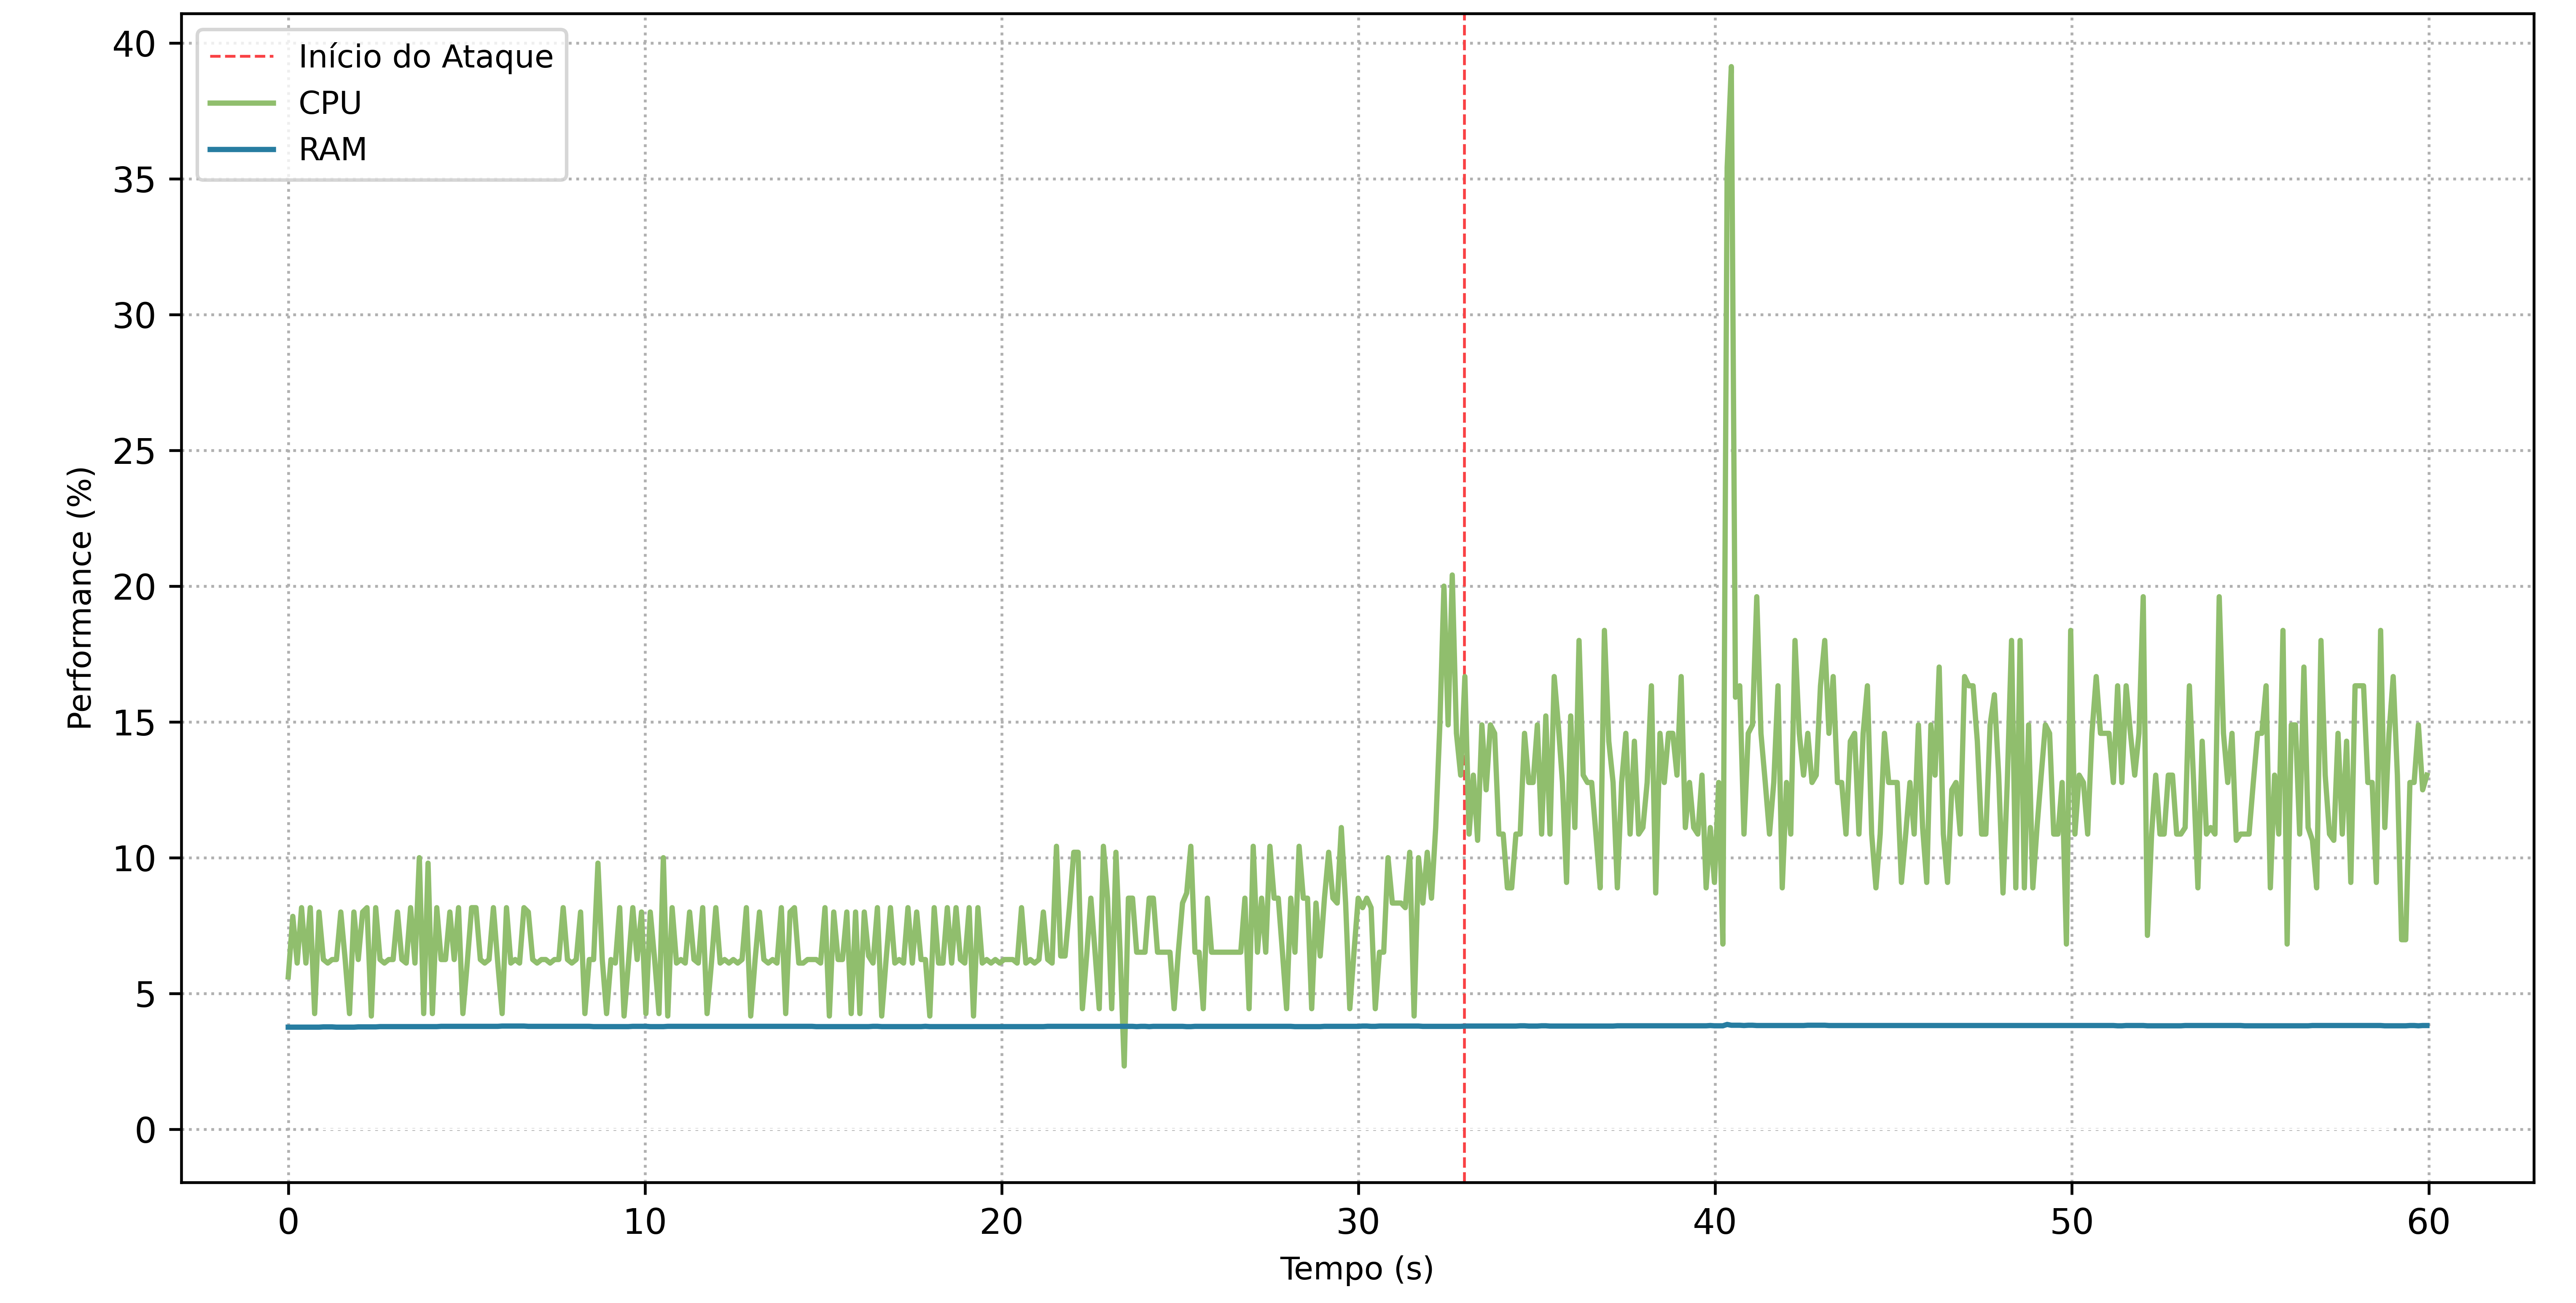
\includegraphics[width=1\textwidth, height=120pt]{USPSC-img/output/cropped/0-dos_open_multiple_secure_channels-perf.png}
        \caption{Desempenho}
    \end{subfigure}%
    \\
    \begin{subfigure}[t]{0.5\textwidth}
        \centering
        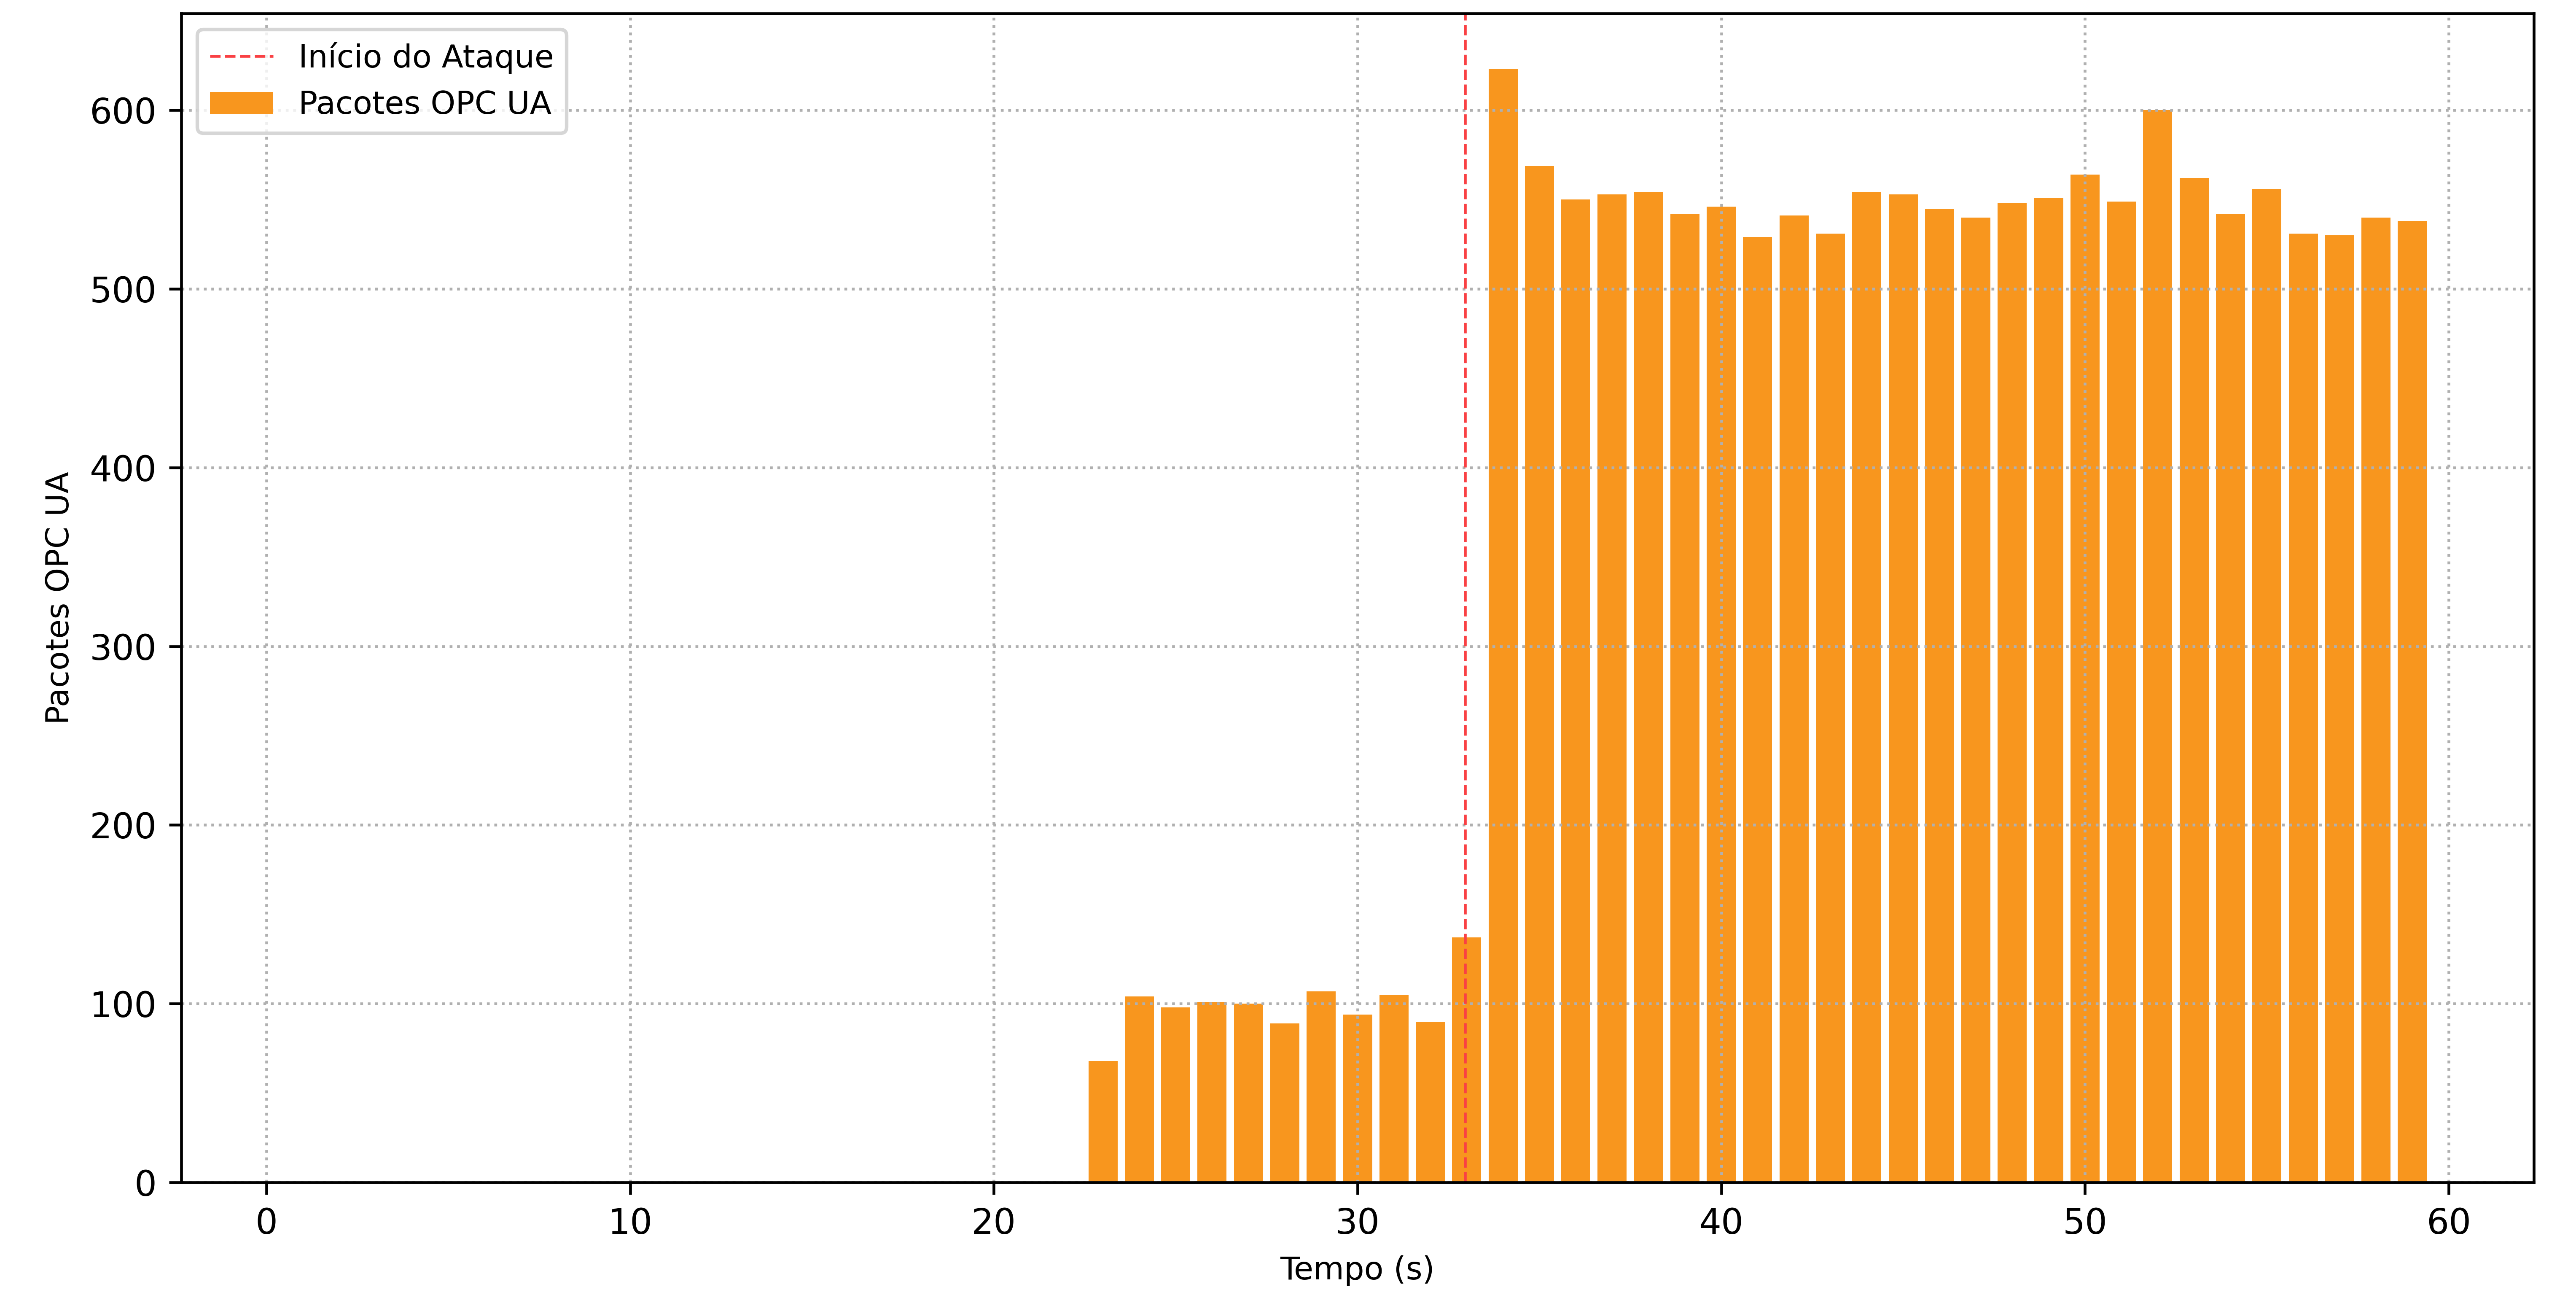
\includegraphics[width=1\textwidth, height=120pt]{USPSC-img/output/cropped/0-dos_open_multiple_secure_channels-pack.png}
        \caption{Pacotes OPC UA}
    \end{subfigure}%
    ~
    \begin{subfigure}[t]{0.5\textwidth}
        \centering
        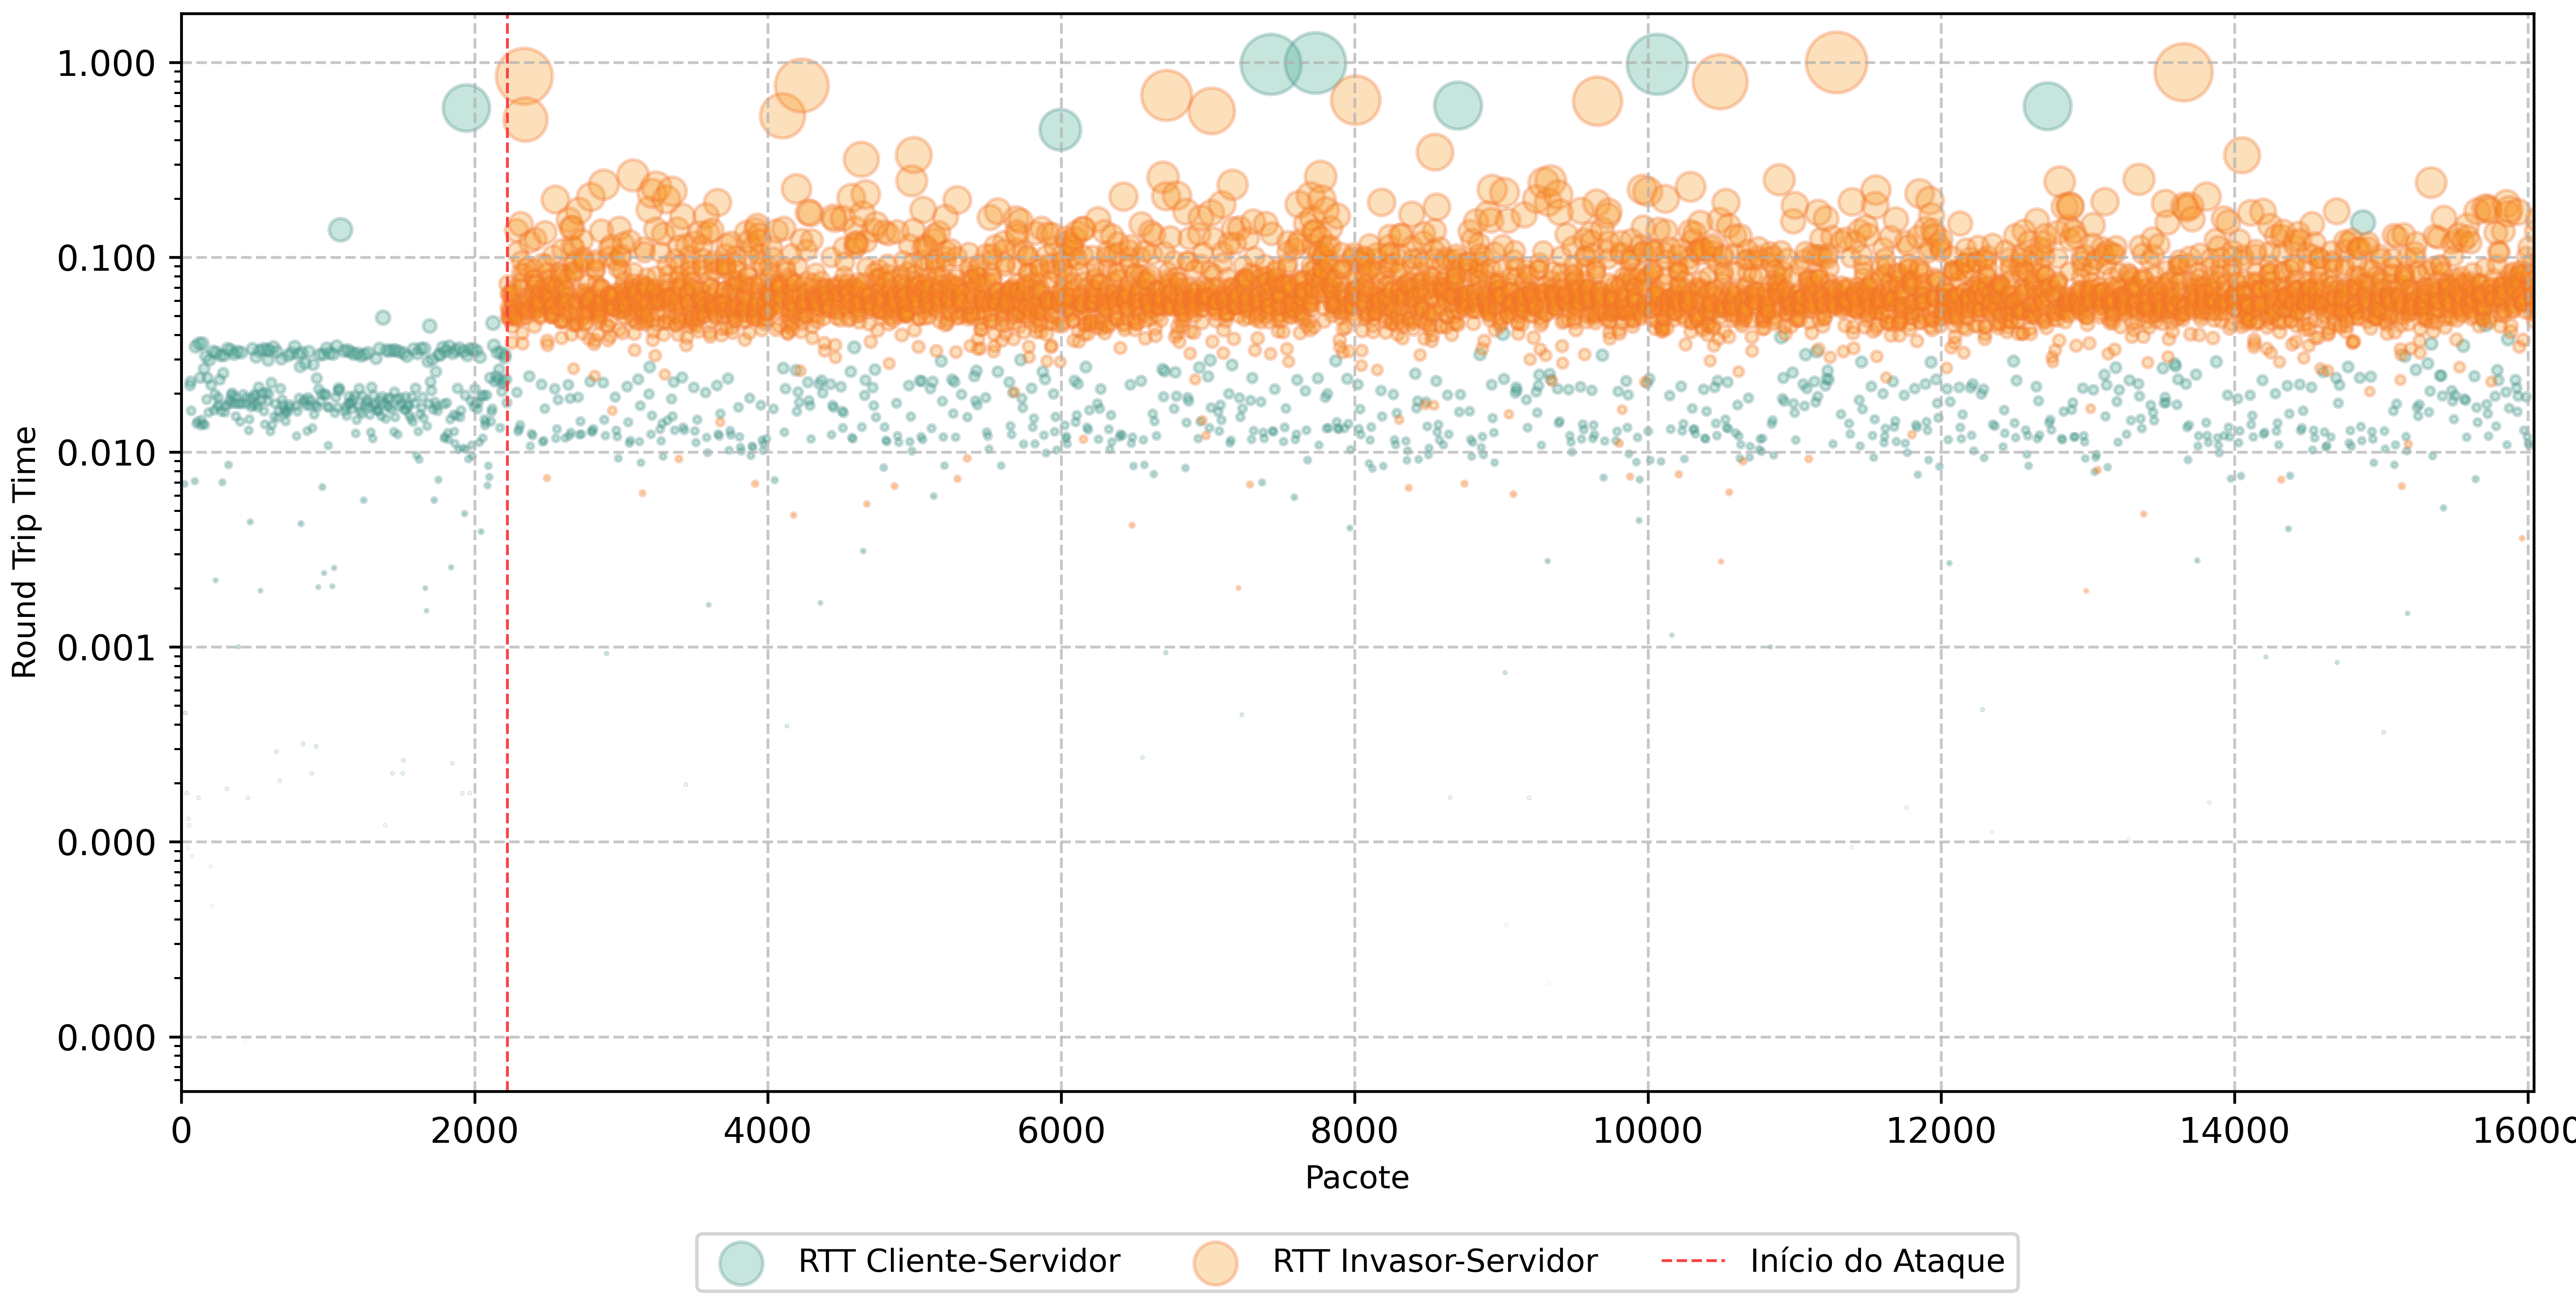
\includegraphics[width=1\textwidth, height=120pt]{USPSC-img/output/cropped/0-dos_open_multiple_secure_channels-rttp.png}
        \caption{RTT por pacote}
    \end{subfigure}%
    % ~
    % \begin{subfigure}[t]{0.5\textwidth}
    %     \centering
    %     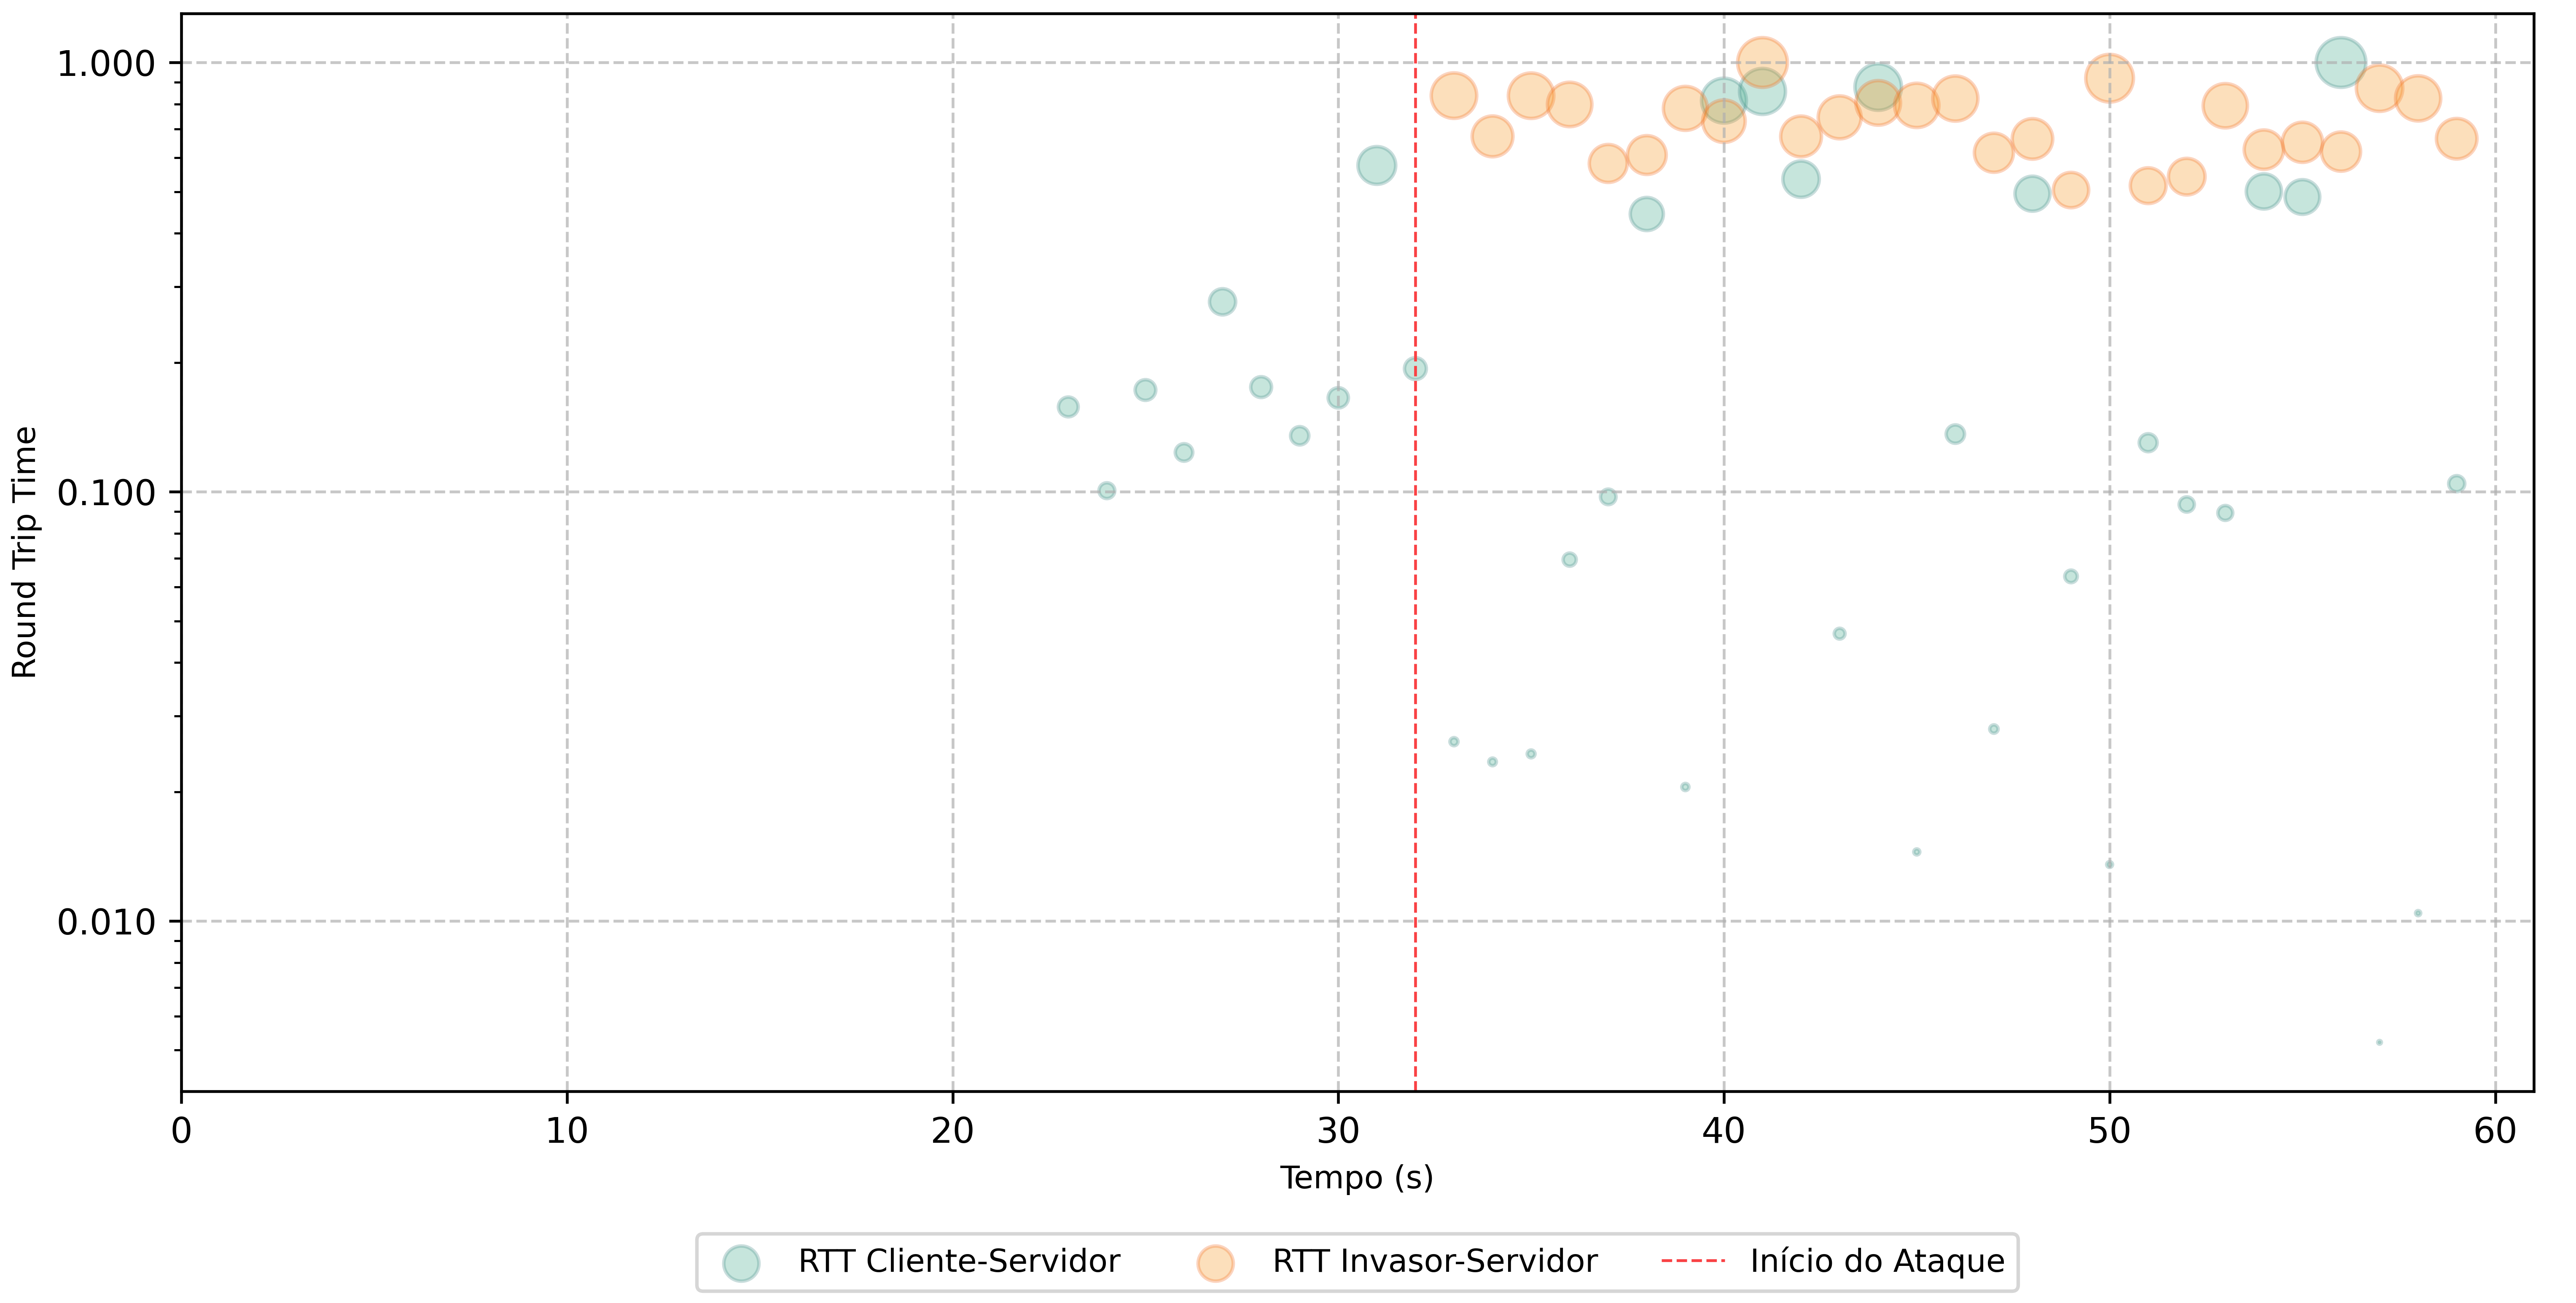
\includegraphics[width=1\textwidth, height=120pt]{USPSC-img/output/cropped/0-dos_open_multiple_secure_channels-rtts.png}
    %     \caption{RTT por segundos}
    % \end{subfigure}%
    \label{fig:0-dos_open_multiple_secure_channels}
    \caption{Gráficos do ataque de DoS pela abertura de múltiplos canais seguros - nível de segurança: `None'.}
\end{figure}

\begin{figure}[htbp!]
    \centering
    \begin{subfigure}[t]{0.5\textwidth}
        \centering
        \includegraphics[width=1\textwidth, height=120pt]{USPSC-img/output/cropped/1-dos_open_multiple_secure_channels-tput.png}
        \caption{\textit{Throughput}}
    \end{subfigure}%
    ~ 
    \begin{subfigure}[t]{0.5\textwidth}
        \centering
        \includegraphics[width=1\textwidth, height=120pt]{USPSC-img/output/cropped/1-dos_open_multiple_secure_channels-perf.png}
        \caption{Desempenho}
    \end{subfigure}%
    \\
    \begin{subfigure}[t]{0.5\textwidth}
        \centering
        \includegraphics[width=1\textwidth, height=120pt]{USPSC-img/output/cropped/1-dos_open_multiple_secure_channels-pack.png}
        \caption{Pacotes OPC UA}
    \end{subfigure}%
    ~
    \begin{subfigure}[t]{0.5\textwidth}
        \centering
        \includegraphics[width=1\textwidth, height=120pt]{USPSC-img/output/cropped/1-dos_open_multiple_secure_channels-rttp.png}
        \caption{RTT por pacote}
    \end{subfigure}%
    % ~
    % \begin{subfigure}[t]{0.5\textwidth}
    %     \centering
    %     \includegraphics[width=1\textwidth, height=120pt]{USPSC-img/output/cropped/1-dos_open_multiple_secure_channels-rtts.png}
    %     \caption{RTT por segundos}
    % \end{subfigure}%
    \label{fig:1-dos_open_multiple_secure_channels}
    \caption{Gráficos do ataque de DoS pela abertura de múltiplos canais seguros - nível de segurança: `Sign'.}
\end{figure}

\begin{figure}[htbp!]
    \centering
    \begin{subfigure}[t]{0.5\textwidth}
        \centering
        \includegraphics[width=1\textwidth, height=120pt]{USPSC-img/output/cropped/2-dos_open_multiple_secure_channels-tput.png}
        \caption{\textit{Throughput}}
    \end{subfigure}%
    ~ 
    \begin{subfigure}[t]{0.5\textwidth}
        \centering
        \includegraphics[width=1\textwidth, height=120pt]{USPSC-img/output/cropped/2-dos_open_multiple_secure_channels-perf.png}
        \caption{Desempenho}
    \end{subfigure}%
    \\
    \begin{subfigure}[t]{0.5\textwidth}
        \centering
        \includegraphics[width=1\textwidth, height=120pt]{USPSC-img/output/cropped/2-dos_open_multiple_secure_channels-pack.png}
        \caption{Pacotes OPC UA}
    \end{subfigure}%
    ~
    \begin{subfigure}[t]{0.5\textwidth}
        \centering
        \includegraphics[width=1\textwidth, height=120pt]{USPSC-img/output/cropped/2-dos_open_multiple_secure_channels-rttp.png}
        \caption{RTT por pacote}
    \end{subfigure}%
    % ~
    % \begin{subfigure}[t]{0.5\textwidth}
    %     \centering
    %     \includegraphics[width=1\textwidth, height=120pt]{USPSC-img/output/cropped/2-dos_open_multiple_secure_channels-rtts.png}
    %     \caption{RTT por segundos}
    % \end{subfigure}%
    \label{fig:2-dos_open_multiple_secure_channels}
    \caption{Gráficos do ataque de DoS pela abertura de múltiplos canais seguros - nível de segurança: `Sign \& Encrypt'.}
\end{figure}

\begin{figure}[htbp!]
    \centering
    \begin{subfigure}[t]{0.5\textwidth}
        \centering
        \includegraphics[width=1\textwidth, height=120pt]{USPSC-img/output/cropped/0-dos_translate_browse_path_call_stack_overflow-tput.png}
        \caption{\textit{Throughput}}
    \end{subfigure}%
    ~ 
    \begin{subfigure}[t]{0.5\textwidth}
        \centering
        \includegraphics[width=1\textwidth, height=120pt]{USPSC-img/output/cropped/0-dos_translate_browse_path_call_stack_overflow-perf.png}
        \caption{Desempenho}
    \end{subfigure}%
    \\
    \begin{subfigure}[t]{0.5\textwidth}
        \centering
        \includegraphics[width=1\textwidth, height=120pt]{USPSC-img/output/cropped/0-dos_translate_browse_path_call_stack_overflow-pack.png}
        \caption{Pacotes OPC UA}
    \end{subfigure}%
    ~
    \begin{subfigure}[t]{0.5\textwidth}
        \centering
        \includegraphics[width=1\textwidth, height=120pt]{USPSC-img/output/cropped/0-dos_translate_browse_path_call_stack_overflow-rttp.png}
        \caption{RTT por pacote}
    \end{subfigure}%
    % ~
    % \begin{subfigure}[t]{0.5\textwidth}
    %     \centering
    %     \includegraphics[width=1\textwidth, height=120pt]{USPSC-img/output/cropped/0-dos_translate_browse_path_call_stack_overflow-rtts.png}
    %     \caption{RTT por segundos}
    % \end{subfigure}%
    \label{fig:0-dos_translate_browse_path_call_stack_overflow}
    \caption{Gráficos do ataque de DoS pela tradução do caminho de navegação - nível de segurança: `None'.}
\end{figure}

\begin{figure}[htbp!]
    \centering
    \begin{subfigure}[t]{0.5\textwidth}
        \centering
        \includegraphics[width=1\textwidth, height=120pt]{USPSC-img/output/cropped/1-dos_translate_browse_path_call_stack_overflow-tput.png}
        \caption{\textit{Throughput}}
    \end{subfigure}%
    ~ 
    \begin{subfigure}[t]{0.5\textwidth}
        \centering
        \includegraphics[width=1\textwidth, height=120pt]{USPSC-img/output/cropped/1-dos_translate_browse_path_call_stack_overflow-perf.png}
        \caption{Desempenho}
    \end{subfigure}%
    \\
    \begin{subfigure}[t]{0.5\textwidth}
        \centering
        \includegraphics[width=1\textwidth, height=120pt]{USPSC-img/output/cropped/1-dos_translate_browse_path_call_stack_overflow-pack.png}
        \caption{Pacotes OPC UA}
    \end{subfigure}%
    ~
    \begin{subfigure}[t]{0.5\textwidth}
        \centering
        \includegraphics[width=1\textwidth, height=120pt]{USPSC-img/output/cropped/1-dos_translate_browse_path_call_stack_overflow-rttp.png}
        \caption{RTT por pacote}
    \end{subfigure}%
    % ~
    % \begin{subfigure}[t]{0.5\textwidth}
    %     \centering
    %     \includegraphics[width=1\textwidth, height=120pt]{USPSC-img/output/cropped/1-dos_translate_browse_path_call_stack_overflow-rtts.png}
    %     \caption{RTT por segundos}
    % \end{subfigure}%
    \label{fig:1-dos_translate_browse_path_call_stack_overflow}
    \caption{Gráficos do ataque de DoS pela tradução do caminho de navegação - nível de segurança: `Sign'.}
\end{figure}

\begin{figure}[htbp!]
    \centering
    \begin{subfigure}[t]{0.5\textwidth}
        \centering
        \includegraphics[width=1\textwidth, height=120pt]{USPSC-img/output/cropped/2-dos_translate_browse_path_call_stack_overflow-tput.png}
        \caption{\textit{Throughput}}
    \end{subfigure}%
    ~ 
    \begin{subfigure}[t]{0.5\textwidth}
        \centering
        \includegraphics[width=1\textwidth, height=120pt]{USPSC-img/output/cropped/2-dos_translate_browse_path_call_stack_overflow-perf.png}
        \caption{Desempenho}
    \end{subfigure}%
    \\
    \begin{subfigure}[t]{0.5\textwidth}
        \centering
        \includegraphics[width=1\textwidth, height=120pt]{USPSC-img/output/cropped/2-dos_translate_browse_path_call_stack_overflow-pack.png}
        \caption{Pacotes OPC UA}
    \end{subfigure}%
    ~
    \begin{subfigure}[t]{0.5\textwidth}
        \centering
        \includegraphics[width=1\textwidth, height=120pt]{USPSC-img/output/cropped/2-dos_translate_browse_path_call_stack_overflow-rttp.png}
        \caption{RTT por pacote}
    \end{subfigure}%
    % ~
    % \begin{subfigure}[t]{0.5\textwidth}
    %     \centering
    %     \includegraphics[width=1\textwidth, height=120pt]{USPSC-img/output/cropped/2-dos_translate_browse_path_call_stack_overflow-rtts.png}
    %     \caption{RTT por segundos}
    % \end{subfigure}%
    \label{fig:2-dos_translate_browse_path_call_stack_overflow}
    \caption{Gráficos do ataque de DoS pela tradução do caminho de navegação - nível de segurança: `Sign \& Encrypt'.}
\end{figure}

\begin{figure}[htbp!]
    \centering
    \begin{subfigure}[t]{0.5\textwidth}
        \centering
        \includegraphics[width=1\textwidth, height=120pt]{USPSC-img/output/cropped/0-mitm_arp-tput.png}
        \caption{\textit{Throughput}}
    \end{subfigure}%
    ~ 
    \begin{subfigure}[t]{0.5\textwidth}
        \centering
        \includegraphics[width=1\textwidth, height=120pt]{USPSC-img/output/cropped/0-mitm_arp-perf.png}
        \caption{Desempenho}
    \end{subfigure}%
    \\
    \begin{subfigure}[t]{0.5\textwidth}
        \centering
        \includegraphics[width=1\textwidth, height=120pt]{USPSC-img/output/cropped/0-mitm_arp-pack.png}
        \caption{Pacotes OPC UA}
    \end{subfigure}%
    ~
    \begin{subfigure}[t]{0.5\textwidth}
        \centering
        \includegraphics[width=1\textwidth, height=120pt]{USPSC-img/output/cropped/0-mitm_arp-rttp.png}
        \caption{RTT por pacote}
    \end{subfigure}%
    % ~
    % \begin{subfigure}[t]{0.5\textwidth}
    %     \centering
    %     \includegraphics[width=1\textwidth, height=120pt]{USPSC-img/output/cropped/0-mitm_arp-rtts.png}
    %     \caption{RTT por segundos}
    % \end{subfigure}%
    \label{fig:0-mitm_arp}
    \caption{Gráficos do ataque de MiTM pela falsificação da tabela ARP - nível de segurança: `None'.}
\end{figure}

\begin{figure}[htbp!]
    \centering
    \begin{subfigure}[t]{0.5\textwidth}
        \centering
        \includegraphics[width=1\textwidth, height=120pt]{USPSC-img/output/cropped/1-mitm_arp-tput.png}
        \caption{\textit{Throughput}}
    \end{subfigure}%
    ~ 
    \begin{subfigure}[t]{0.5\textwidth}
        \centering
        \includegraphics[width=1\textwidth, height=120pt]{USPSC-img/output/cropped/1-mitm_arp-perf.png}
        \caption{Desempenho}
    \end{subfigure}%
    \\
    \begin{subfigure}[t]{0.5\textwidth}
        \centering
        \includegraphics[width=1\textwidth, height=120pt]{USPSC-img/output/cropped/1-mitm_arp-pack.png}
        \caption{Pacotes OPC UA}
    \end{subfigure}%
    ~
    \begin{subfigure}[t]{0.5\textwidth}
        \centering
        \includegraphics[width=1\textwidth, height=120pt]{USPSC-img/output/cropped/1-mitm_arp-rttp.png}
        \caption{RTT por pacote}
    \end{subfigure}%
    % ~
    % \begin{subfigure}[t]{0.5\textwidth}
    %     \centering
    %     \includegraphics[width=1\textwidth, height=120pt]{USPSC-img/output/cropped/1-mitm_arp-rtts.png}
    %     \caption{RTT por segundos}
    % \end{subfigure}%
    \label{fig:1-mitm_arp}
    \caption{Gráficos do ataque de MiTM pela falsificação da tabela ARP - nível de segurança: `Sign'.}
\end{figure}

\begin{figure}[htbp!]
    \centering
    \begin{subfigure}[t]{0.5\textwidth}
        \centering
        \includegraphics[width=1\textwidth, height=120pt]{USPSC-img/output/cropped/2-mitm_arp-tput.png}
        \caption{\textit{Throughput}}
    \end{subfigure}%
    ~ 
    \begin{subfigure}[t]{0.5\textwidth}
        \centering
        \includegraphics[width=1\textwidth, height=120pt]{USPSC-img/output/cropped/2-mitm_arp-perf.png}
        \caption{Desempenho}
    \end{subfigure}%
    \\
    \begin{subfigure}[t]{0.5\textwidth}
        \centering
        \includegraphics[width=1\textwidth, height=120pt]{USPSC-img/output/cropped/2-mitm_arp-pack.png}
        \caption{Pacotes OPC UA}
    \end{subfigure}%
    ~
    \begin{subfigure}[t]{0.5\textwidth}
        \centering
        \includegraphics[width=1\textwidth, height=120pt]{USPSC-img/output/cropped/2-mitm_arp-rttp.png}
        \caption{RTT por pacote}
    \end{subfigure}%
    % ~
    % \begin{subfigure}[t]{0.5\textwidth}
    %     \centering
    %     \includegraphics[width=1\textwidth, height=120pt]{USPSC-img/output/cropped/2-mitm_arp-rtts.png}
    %     \caption{RTT por segundos}
    % \end{subfigure}%
    \label{fig:2-mitm_arp}
    \caption{Gráficos do ataque de MiTM pela falsificação da tabela ARP - nível de segurança: `Sign \& Encrypt'.}
\end{figure}

\begin{figure}[htbp!]
    \centering
    \begin{subfigure}[t]{0.5\textwidth}
        \centering
        \includegraphics[width=1\textwidth, height=120pt]{USPSC-img/output/cropped/0-mitm_port-tput.png}
        \caption{\textit{Throughput}}
    \end{subfigure}%
    ~ 
    \begin{subfigure}[t]{0.5\textwidth}
        \centering
        \includegraphics[width=1\textwidth, height=120pt]{USPSC-img/output/cropped/0-mitm_port-perf.png}
        \caption{Desempenho}
    \end{subfigure}%
    \\
    \begin{subfigure}[t]{0.5\textwidth}
        \centering
        \includegraphics[width=1\textwidth, height=120pt]{USPSC-img/output/cropped/0-mitm_port-pack.png}
        \caption{Pacotes OPC UA}
    \end{subfigure}%
    ~
    \begin{subfigure}[t]{0.5\textwidth}
        \centering
        \includegraphics[width=1\textwidth, height=120pt]{USPSC-img/output/cropped/0-mitm_port-rttp.png}
        \caption{RTT por pacote}
    \end{subfigure}%
    % ~
    % \begin{subfigure}[t]{0.5\textwidth}
    %     \centering
    %     \includegraphics[width=1\textwidth, height=120pt]{USPSC-img/output/cropped/0-mitm_port-rtts.png}
    %     \caption{RTT por segundos}
    % \end{subfigure}%
    \label{fig:0-mitm_port}
    \caption{Gráficos do ataque de MiTM pelo roubo de portas - nível de segurança: `None'.}
\end{figure}

\begin{figure}[htbp!]
    \centering
    \begin{subfigure}[t]{0.5\textwidth}
        \centering
        \includegraphics[width=1\textwidth, height=120pt]{USPSC-img/output/cropped/1-mitm_port-tput.png}
        \caption{\textit{Throughput}}
    \end{subfigure}%
    ~ 
    \begin{subfigure}[t]{0.5\textwidth}
        \centering
        \includegraphics[width=1\textwidth, height=120pt]{USPSC-img/output/cropped/1-mitm_port-perf.png}
        \caption{Desempenho}
    \end{subfigure}%
    \\
    \begin{subfigure}[t]{0.5\textwidth}
        \centering
        \includegraphics[width=1\textwidth, height=120pt]{USPSC-img/output/cropped/1-mitm_port-pack.png}
        \caption{Pacotes OPC UA}
    \end{subfigure}%
    ~
    \begin{subfigure}[t]{0.5\textwidth}
        \centering
        \includegraphics[width=1\textwidth, height=120pt]{USPSC-img/output/cropped/1-mitm_port-rttp.png}
        \caption{RTT por pacote}
    \end{subfigure}%
    % ~
    % \begin{subfigure}[t]{0.5\textwidth}
    %     \centering
    %     \includegraphics[width=1\textwidth, height=120pt]{USPSC-img/output/cropped/1-mitm_port-rtts.png}
    %     \caption{RTT por segundos}
    % \end{subfigure}%
    \label{fig:1-mitm_port}
    \caption{Gráficos do ataque de MiTM pelo roubo de portas - nível de segurança: `Sign'.}
\end{figure}

\begin{figure}[htbp!]
    \centering
    \begin{subfigure}[t]{0.5\textwidth}
        \centering
        \includegraphics[width=1\textwidth, height=120pt]{USPSC-img/output/cropped/2-mitm_port-tput.png}
        \caption{\textit{Throughput}}
    \end{subfigure}%
    ~ 
    \begin{subfigure}[t]{0.5\textwidth}
        \centering
        \includegraphics[width=1\textwidth, height=120pt]{USPSC-img/output/cropped/2-mitm_port-perf.png}
        \caption{Desempenho}
    \end{subfigure}%
    \\
    \begin{subfigure}[t]{0.5\textwidth}
        \centering
        \includegraphics[width=1\textwidth, height=120pt]{USPSC-img/output/cropped/2-mitm_port-pack.png}
        \caption{Pacotes OPC UA}
    \end{subfigure}%
    ~
    \begin{subfigure}[t]{0.5\textwidth}
        \centering
        \includegraphics[width=1\textwidth, height=120pt]{USPSC-img/output/cropped/2-mitm_port-rttp.png}
        \caption{RTT por pacote}
    \end{subfigure}%
    % ~
    % \begin{subfigure}[t]{0.5\textwidth}
    %     \centering
    %     \includegraphics[width=1\textwidth, height=120pt]{USPSC-img/output/cropped/2-mitm_port-rtts.png}
    %     \caption{RTT por segundos}
    % \end{subfigure}%
    \label{fig:2-mitm_port}
    \caption{Gráficos do ataque de MiTM pelo roubo de portas - nível de segurança: `Sign \& Encrypt'.}
\end{figure}

\end{apendicesenv}
% ---